% !TeX program = xelatex
\documentclass[UTF8,a4paper,zihao=-4,fontset=windows]{ctexart}
\usepackage[margin=21mm,headheight=15pt]{geometry}
\usepackage{amsmath,amssymb,graphicx,xcolor,needspace,longtable,booktabs,fancyhdr}
\usepackage[unicode,hidelinks]{hyperref}
\setlength{\parindent}{0pt}
\setlength{\parskip}{4pt}
\setlength{\emergencystretch}{4em}
\linespread{1.13}\raggedbottom\raggedright
\pagestyle{fancy}\fancyhf{}
\fancyhead[L]{湘教版必修第一册：期中教师资料}
\fancyhead[R]{答案与知识点}\fancyfoot[C]{\thepage}
\graphicspath{{../TeX题库/}}
\newcommand{\subq}[1]{\par\Needspace{2\baselineskip}\noindent（#1）\quad}
\newcommand{\choice}[1]{\par\noindent #1.\quad}
\newcommand{\blank}{\underline{\hspace{1.3cm}}}
\newcommand{\bankfig}[2]{\begin{center}\includegraphics[width=#2\linewidth]{../TeX题库/figures/#1.png}\end{center}}
\newcommand{\itemhead}[2]{\par\Needspace{8\baselineskip}\medskip\hrule\smallskip\textbf{#1}\par{\footnotesize\ttfamily #2}\par}
\newcommand{\field}[2]{\par\textbf{#1：}#2\par}
\hypersetup{pdfauthor={教学资料整理}}

\begin{document}
\begin{center}{\LARGE 期中教材题库：答案与知识点}\par\medskip
{\large 湘教版必修第一册第1—3章、4.1—4.2}\end{center}
本册为教师配套资料，共368个主标签条目（第1章107、第2章104、第3章92、第4章期中部分65）。题干、答案与数学公式均可编辑，必要原配图单独引用。学生卷及原题库未改动。
\par 252个练习、习题和复习题参照所给答案册的相关题组重新计算；70个例题参考教材原解；其余46个思考、小结、案例、实验补写参考回应。答案册有旧版小问及题号变化，不将相关题组伪装成逐题完全匹配。证明题给出关键推理，作图题给出解析式、关键点或明确作图规则；另附25幅答案图，其中24幅按数学关系绘制，1幅为已核对的答案册补图。
\par 知识点依所给《教材帮》的实际内容匹配，其章节与湘教版不同（例如幂函数位于教材帮第3章），不可直接按章号对套。每条给出书内页码及PDF页序；知识总表另册按本次考试范围整理。
\par 本册是编写并验算的教师参考解答，尚未获得教师签核；题干原先的转写复核状态不因补答案而自动改变。重点复核：教材p.58甲车刹车题条件不足，p.72蓄水量题仅有非唯一的读图估计。分歧说明随题列出。
\par 定位说明：湘教版正文PDF页序=教材页码+7；《教材帮》正文PDF页序=书内页码+9；答案册PDF页序=册内页码+1。所有页序从1开始。
\tableofcontents\clearpage
\section{第1章 集合与逻辑}
\itemhead{1.1 思考 · 未编号题组（教材p.2）}{XJ-B1-C01-TH-P002-Y0577}
\label{XJ-B1-C01-TH-P002-Y0577}
{\footnotesize 湘教版教材p.2 / PDF第9页 / 1.1 思考 / 未编号题组}
\field{原题}{下面第一句话里的“是”的含义相当于“$=$”，另外两句话里的“是”的含义是什么？
\subq{1}关羽千里走单骑的坐骑是赤兔马；
\subq{2}赤兔马是红马；
\subq{3}红马是马。}
\field{参考答案}{（2）表示赤兔马属于红马这一集合；（3）表示红马组成的集合包含于马组成的集合。分别对应元素与集合、集合与集合的关系。}
{\small \field{关联知识}{S01 集合、元素与常用数集（教材帮p.1、2 / PDF10、11）；S03 子集、真子集与集合相等（教材帮p.11、12、13 / PDF20、21、22）}
\field{方法与易错点}{先辨认研究对象和数集范围，再代入定义判断；含参集合逐个来源分类。 易错：把自然数集误作正整数集；混淆元素和单元素集合；候选参数造成元素重复。}
\field{答案依据}{答案册未提供本栏目的独立对应答案；依据原题、教材概念补写参考回应。开放性总结不设唯一数值答案。}}

\itemhead{1.1 例题 · 例题1（教材p.3）}{XJ-B1-C01-EX-P003-Y0620}
\label{XJ-B1-C01-EX-P003-Y0620}
{\footnotesize 湘教版教材p.3 / PDF第10页 / 1.1 例题 / 例题1}
\field{原题}{设 $L(A,B)$ 表示直线 $AB$ 上全体点组成的集合，则 $P\in L(A,B)$ 的含义是什么？}
\field{参考答案}{$P$ 是直线 $AB$ 上的一个点。}
{\small \field{关联知识}{S01 集合、元素与常用数集（教材帮p.1、2 / PDF10、11）}
\field{方法与易错点}{先辨认研究对象和数集范围，再代入定义判断；含参集合逐个来源分类。 易错：把自然数集误作正整数集；混淆元素和单元素集合；候选参数造成元素重复。}
\field{答案依据}{例题原解位置：湘教版教材p.3及题库原图；独立编写可编辑参考解答。答案册此部分主要收练习、习题，不伪造例题答案册位置。}}

\itemhead{1.1 例题 · 例题2（教材p.3）}{XJ-B1-C01-EX-P003-Y1223}
\label{XJ-B1-C01-EX-P003-Y1223}
{\footnotesize 湘教版教材p.3 / PDF第10页 / 1.1 例题 / 例题2}
\field{原题}{下列集合中哪些是有限集？哪些是无限集？
\subq{1}一元二次方程 $x^2+1=0$ 的全体实根组成的集合 $A$；
\subq{2}所有素数（即质数）组成的集合 $B$；
\subq{3}所有矩形组成的集合 $C$；
\subq{4}所有亚洲国家组成的集合 $D$。}
\field{参考答案}{$A=\varnothing$，是有限集；$B,C$ 是无限集；$D$ 是有限集。}
{\small \field{关联知识}{S01 集合、元素与常用数集（教材帮p.1、2 / PDF10、11）}
\field{方法与易错点}{先辨认研究对象和数集范围，再代入定义判断；含参集合逐个来源分类。 易错：把自然数集误作正整数集；混淆元素和单元素集合；候选参数造成元素重复。}
\field{答案依据}{例题原解位置：湘教版教材p.3及题库原图；独立编写可编辑参考解答。答案册此部分主要收练习、习题，不伪造例题答案册位置。}}

\itemhead{p.4 练习 · 第1题（教材p.4）}{XJ-B1-C01-PR-P004-Y0218}
\label{XJ-B1-C01-PR-P004-Y0218}
{\footnotesize 湘教版教材p.4 / PDF第11页 / p.4 练习 / 第1题}
\field{原题}{使用“$\in$”“$\notin$”填空：
\subq{1}“255 是正整数”即 $255\blank\mathbb Z_+$；
\subq{2}“$\sqrt2$ 不是有理数”即 $\sqrt2\blank\mathbb Q$；
\subq{3}“1.414 是正实数”即 $1.414\blank\mathbb R_+$；
\subq{4}“$x$ 是负实数”即 $x\blank\mathbb R_-$。}
\field{参考答案}{依次为 $\in,\notin,\in,\in$。按题库所据原教材的四小问作答，不能照抄答案册此处五小问的次序。}
\field{核对说明}{版本小问变化：答案册PDF4有五小问；现教材四小问，按原题的对象和符号作答。}
{\small \field{关联知识}{S01 集合、元素与常用数集（教材帮p.1、2 / PDF10、11）}
\field{方法与易错点}{先辨认研究对象和数集范围，再代入定义判断；含参集合逐个来源分类。 易错：把自然数集误作正整数集；混淆元素和单元素集合；候选参数造成元素重复。}
\field{答案依据}{答案册相关题组：PDF第4页（册内页3）；按当前题库原题逐项重算，不按旧版题号机械对套。}}

\itemhead{p.4 练习 · 第2题（教材p.4）}{XJ-B1-C01-PR-P004-Y0443}
\label{XJ-B1-C01-PR-P004-Y0443}
{\footnotesize 湘教版教材p.4 / PDF第11页 / p.4 练习 / 第2题}
\field{原题}{下列集合中哪些是有限集？哪些是无限集？
\subq{1}不等式 $5x-3>7$ 的所有实数解组成的集合；
\subq{2}一元二次方程 $x^2+x+1=0$ 的全体实根组成的集合；
\subq{3}中国古代四大发明组成的集合；
\subq{4}二次函数 $y=3x^2+4$ 的函数值组成的集合。}
\field{参考答案}{（1）（4）无限集；（2）（3）有限集。（2）为空集，也属于有限集。}
{\small \field{关联知识}{S01 集合、元素与常用数集（教材帮p.1、2 / PDF10、11）}
\field{方法与易错点}{先辨认研究对象和数集范围，再代入定义判断；含参集合逐个来源分类。 易错：把自然数集误作正整数集；混淆元素和单元素集合；候选参数造成元素重复。}
\field{答案依据}{答案册相关题组：PDF第4页（册内页3）；按当前题库原题逐项重算，不按旧版题号机械对套。}}

\itemhead{1.1 例题 · 例题3（教材p.4）}{XJ-B1-C01-EX-P004-Y1108}
\label{XJ-B1-C01-EX-P004-Y1108}
{\footnotesize 湘教版教材p.4 / PDF第11页 / 1.1 例题 / 例题3}
\field{原题}{用列举法表示下列集合：
\subq{1}由方程 $x^2-1=0$ 的所有实数解构成的集合 $S$；
\subq{2}平方不大于 9 的所有整数构成的集合 $P$。}
\field{参考答案}{（1）$S=\{-1,1\}$；（2）$P=\{-3,-2,-1,0,1,2,3\}$。}
{\small \field{关联知识}{S02 集合表示、区间与数集点集（教材帮p.2、3、4 / PDF11、12、13）}
\field{方法与易错点}{先求出约束的解，再选列举法或描述法，必要时在数轴或坐标系中表示。 易错：遗漏0或负整数；将一个有序数对拆成两个元素；区间端点误取。}
\field{答案依据}{例题原解位置：湘教版教材p.4及题库原图；独立编写可编辑参考解答。答案册此部分主要收练习、习题，不伪造例题答案册位置。}}

\itemhead{1.1 例题 · 例题4（教材p.5）}{XJ-B1-C01-EX-P005-Y0448}
\label{XJ-B1-C01-EX-P005-Y0448}
{\footnotesize 湘教版教材p.5 / PDF第12页 / 1.1 例题 / 例题4}
\field{原题}{选择适当方法表示下列集合：
\subq{1}由大于 20 且小于 30 的所有实数组成的集合 $A$；
\subq{2}由方程 $x^2+y^2=4$ 的所有整数解 $(x,y)$ 组成的集合 $B$。}
\field{参考答案}{（1）$A=\{x\in\mathbb R\mid20<x<30\}$；（2）$B=\{(2,0),(-2,0),(0,2),(0,-2)\}$。}
{\small \field{关联知识}{S02 集合表示、区间与数集点集（教材帮p.2、3、4 / PDF11、12、13）}
\field{方法与易错点}{先求出约束的解，再选列举法或描述法，必要时在数轴或坐标系中表示。 易错：遗漏0或负整数；将一个有序数对拆成两个元素；区间端点误取。}
\field{答案依据}{例题原解位置：湘教版教材p.5及题库原图；独立编写可编辑参考解答。答案册此部分主要收练习、习题，不伪造例题答案册位置。}}

\itemhead{1.1 例题 · 例题5（教材p.5）}{XJ-B1-C01-EX-P005-Y1339}
\label{XJ-B1-C01-EX-P005-Y1339}
{\footnotesize 湘教版教材p.5 / PDF第12页 / 1.1 例题 / 例题5}
\field{原题}{用区间表示下列集合：
\subq{1}$\{x\in\mathbb R\mid -2\le x\le4\}$；
\subq{2}$\{t\in\mathbb R\mid t<a,\ a\in\mathbb R\}$；
\subq{3}$\{u\in\mathbb R\mid u\ge0\}$。}
\field{参考答案}{（1）$[-2,4]$；（2）$(-\infty,a)$；（3）$[0,+\infty)$。}
{\small \field{关联知识}{S02 集合表示、区间与数集点集（教材帮p.2、3、4 / PDF11、12、13）}
\field{方法与易错点}{先求出约束的解，再选列举法或描述法，必要时在数轴或坐标系中表示。 易错：遗漏0或负整数；将一个有序数对拆成两个元素；区间端点误取。}
\field{答案依据}{例题原解位置：湘教版教材p.5及题库原图；独立编写可编辑参考解答。答案册此部分主要收练习、习题，不伪造例题答案册位置。}}

\itemhead{p.6 练习 · 第1题（教材p.6）}{XJ-B1-C01-PR-P006-Y0217}
\label{XJ-B1-C01-PR-P006-Y0217}
{\footnotesize 湘教版教材p.6 / PDF第13页 / p.6 练习 / 第1题}
\field{原题}{用列举法表示下列集合：
\subq{1}$\{\text{不超过 30 的素数}\}$；
\subq{2}$\{\text{五边形 }ABCDE\text{ 的对角线}\}$；
\subq{3}$\{60\text{ 的正约数}\}$；
\subq{4}$\{(x,y)\mid x+2y=6,\ x\in\mathbb N,\ y\in\mathbb N\}$。}
\field{参考答案}{（1）$\{2,3,5,7,11,13,17,19,23,29\}$；（2）$\{AC,AD,BD,BE,CE\}$；（3）$\{1,2,3,4,5,6,10,12,15,20,30,60\}$；（4）$\{(6,0),(4,1),(2,2),(0,3)\}$。}
{\small \field{关联知识}{S02 集合表示、区间与数集点集（教材帮p.2、3、4 / PDF11、12、13）}
\field{方法与易错点}{先求出约束的解，再选列举法或描述法，必要时在数轴或坐标系中表示。 易错：遗漏0或负整数；将一个有序数对拆成两个元素；区间端点误取。}
\field{答案依据}{答案册相关题组：PDF第4页（册内页3）；按当前题库原题逐项重算，不按旧版题号机械对套。}}

\itemhead{p.6 练习 · 第2题（教材p.6）}{XJ-B1-C01-PR-P006-Y0346}
\label{XJ-B1-C01-PR-P006-Y0346}
{\footnotesize 湘教版教材p.6 / PDF第13页 / p.6 练习 / 第2题}
\field{原题}{用描述法表示下列集合：
\subq{1}$\{1,3,5,7,9\}$；
\subq{2}不等式 $3x>2$ 的解集；
\subq{3}$\{3,5,7,11,13,17,19\}$。}
\field{参考答案}{（1）$\{2k+1\mid k\in\mathbb Z,0\le k\le4\}$；（2）$\{x\in\mathbb R\mid3x>2\}$；（3）$\{x\mid x\text{为小于20的奇素数}\}$。}
{\small \field{关联知识}{S02 集合表示、区间与数集点集（教材帮p.2、3、4 / PDF11、12、13）}
\field{方法与易错点}{先求出约束的解，再选列举法或描述法，必要时在数轴或坐标系中表示。 易错：遗漏0或负整数；将一个有序数对拆成两个元素；区间端点误取。}
\field{答案依据}{答案册相关题组：PDF第4页（册内页3）；按当前题库原题逐项重算，不按旧版题号机械对套。}}

\itemhead{p.6 练习 · 第3题（教材p.6）}{XJ-B1-C01-PR-P006-Y0475}
\label{XJ-B1-C01-PR-P006-Y0475}
{\footnotesize 湘教版教材p.6 / PDF第13页 / p.6 练习 / 第3题}
\field{原题}{用区间表示下列集合：
\subq{1}$\{x\in\mathbb R\mid 3-x>5\}$；
\subq{2}$\{x\in\mathbb R\mid x+3>1\text{ 且 }5-x>2\}$。}
\field{参考答案}{（1）$(-\infty,-2)$；（2）$(-2,3)$。}
{\small \field{关联知识}{S02 集合表示、区间与数集点集（教材帮p.2、3、4 / PDF11、12、13）}
\field{方法与易错点}{先求出约束的解，再选列举法或描述法，必要时在数轴或坐标系中表示。 易错：遗漏0或负整数；将一个有序数对拆成两个元素；区间端点误取。}
\field{答案依据}{答案册相关题组：PDF第4页（册内页3）；按当前题库原题逐项重算，不按旧版题号机械对套。}}

\itemhead{1.1 思考 · 未编号题组（教材p.6）}{XJ-B1-C01-TH-P006-Y0849}
\label{XJ-B1-C01-TH-P006-Y0849}
{\footnotesize 湘教版教材p.6 / PDF第13页 / 1.1 思考 / 未编号题组}
\field{原题}{观察下列各组集合，你能发现两个集合间的关系吗？
\subq{1}$A=\{3,5,7\}$，$B=(2,8]$；
\subq{2}$A=\{\text{等边三角形}\}$，$B=\{\text{等腰三角形}\}$。}
\field{参考答案}{两组均有 $A\subsetneq B$，即 $A$ 中每个元素都属于 $B$，而 $B$ 中还有不属于 $A$ 的元素。}
{\small \field{关联知识}{S03 子集、真子集与集合相等（教材帮p.11、12、13 / PDF20、21、22）}
\field{方法与易错点}{用逐元素检验或数轴包含；参数题先确认是否允许空集，再讨论端点。 易错：遗漏空集；把元素个数相等当作集合相等；把子集符号当作属于符号。}
\field{答案依据}{答案册未提供本栏目的独立对应答案；依据原题、教材概念补写参考回应。开放性总结不设唯一数值答案。}}

\itemhead{1.1 例题 · 例题6（教材p.7）}{XJ-B1-C01-EX-P007-Y0656}
\label{XJ-B1-C01-EX-P007-Y0656}
{\footnotesize 湘教版教材p.7 / PDF第14页 / 1.1 例题 / 例题6}
\field{原题}{设 $S=\{a,b,c\}$，写出 $S$ 的所有子集，并指出哪些是它的真子集。}
\field{参考答案}{子集为 $\varnothing,\{a\},\{b\},\{c\},\{a,b\},\{a,c\},\{b,c\},S$，共8个；除 $S$ 本身外，其余7个都是真子集。}
{\small \field{关联知识}{S03 子集、真子集与集合相等（教材帮p.11、12、13 / PDF20、21、22）}
\field{方法与易错点}{用逐元素检验或数轴包含；参数题先确认是否允许空集，再讨论端点。 易错：遗漏空集；把元素个数相等当作集合相等；把子集符号当作属于符号。}
\field{答案依据}{例题原解位置：湘教版教材p.7及题库原图；独立编写可编辑参考解答。答案册此部分主要收练习、习题，不伪造例题答案册位置。}}

\itemhead{1.1 思考 · 未编号题组（教材p.7）}{XJ-B1-C01-TH-P007-Y1130}
\label{XJ-B1-C01-TH-P007-Y1130}
{\footnotesize 湘教版教材p.7 / PDF第14页 / 1.1 思考 / 未编号题组}
\field{原题}{观察下列各组中的三个集合，你能发现它们之间的关系吗？
\subq{1}$U=\{1,2,3,4,5,6\}$，$A=\{1,3,5\}$，$B=\{2,4,6\}$；
\subq{2}$U=\{\text{三角形}\}$，$A=\{\text{锐角三角形，钝角三角形}\}$，$B=\{\text{直角三角形}\}$。}
\field{参考答案}{两组均满足 $A\cap B=\varnothing,A\cup B=U$，故 $B=\complement_U A$，$A=\complement_U B$。}
{\small \field{关联知识}{S05 全集、补集与德摩根律（教材帮p.21 / PDF30）}
\field{方法与易错点}{标出全集内的已知集合，取剩余区域，先算括号内部再补集。 易错：忘记全集范围；对“且”的否定仍写“且”；漏闭端点。}
\field{答案依据}{答案册未提供本栏目的独立对应答案；依据原题、教材概念补写参考回应。开放性总结不设唯一数值答案。}}

\itemhead{1.1 例题 · 例题7（教材p.8）}{XJ-B1-C01-EX-P008-Y0280}
\label{XJ-B1-C01-EX-P008-Y0280}
{\footnotesize 湘教版教材p.8 / PDF第15页 / 1.1 例题 / 例题7}
\field{原题}{设 $U=\{x\in\mathbb Z\mid x\in(0,12]\}$，$A=\{x\in\mathbb N\mid0<x<6\}$，$B=\{x\in\mathbb Z\mid x\in[7,11]\}$，求 $\complement_U A$ 和 $\complement_U B$。}
\field{参考答案}{$\complement_U A=\{6,7,8,9,10,11,12\}$；$\complement_U B=\{1,2,3,4,5,6,12\}$。}
{\small \field{关联知识}{S05 全集、补集与德摩根律（教材帮p.21 / PDF30）}
\field{方法与易错点}{标出全集内的已知集合，取剩余区域，先算括号内部再补集。 易错：忘记全集范围；对“且”的否定仍写“且”；漏闭端点。}
\field{答案依据}{例题原解位置：湘教版教材p.8及题库原图；独立编写可编辑参考解答。答案册此部分主要收练习、习题，不伪造例题答案册位置。}}

\itemhead{1.1 例题 · 例题8（教材p.8）}{XJ-B1-C01-EX-P008-Y0515}
\label{XJ-B1-C01-EX-P008-Y0515}
{\footnotesize 湘教版教材p.8 / PDF第15页 / 1.1 例题 / 例题8}
\field{原题}{把区间 $[0,1]$ 看成全集，写出它的下列子集的补集：
\[A=(0,1),\quad B=\{1\},\quad C=\{x\mid0\le x<0.5\},\quad D=[0,1].\]}
\field{参考答案}{依次为 $\{0,1\},[0,1),[0.5,1],\varnothing$。}
{\small \field{关联知识}{S05 全集、补集与德摩根律（教材帮p.21 / PDF30）}
\field{方法与易错点}{标出全集内的已知集合，取剩余区域，先算括号内部再补集。 易错：忘记全集范围；对“且”的否定仍写“且”；漏闭端点。}
\field{答案依据}{例题原解位置：湘教版教材p.8及题库原图；独立编写可编辑参考解答。答案册此部分主要收练习、习题，不伪造例题答案册位置。}}

\itemhead{p.8 练习 · 第1题（教材p.8）}{XJ-B1-C01-PR-P008-Y0877}
\label{XJ-B1-C01-PR-P008-Y0877}
{\footnotesize 湘教版教材p.8 / PDF第15页 / p.8 练习 / 第1题}
\field{原题}{设 $Y$ 是由 6 的全体正约数组成的集合，写出 $Y$ 的所有子集。}
\field{参考答案}{$Y=\{1,2,3,6\}$。子集为 $\varnothing$；$\{1\},\{2\},\{3\},\{6\}$；$\{1,2\},\{1,3\},\{1,6\},\{2,3\},\{2,6\},\{3,6\}$；$\{1,2,3\},\{1,2,6\},\{1,3,6\},\{2,3,6\}$；$Y$，共16个。}
{\small \field{关联知识}{S03 子集、真子集与集合相等（教材帮p.11、12、13 / PDF20、21、22）}
\field{方法与易错点}{用逐元素检验或数轴包含；参数题先确认是否允许空集，再讨论端点。 易错：遗漏空集；把元素个数相等当作集合相等；把子集符号当作属于符号。}
\field{答案依据}{答案册相关题组：PDF第4页（册内页3）；按当前题库原题逐项重算，不按旧版题号机械对套。}}

\itemhead{p.8 练习 · 第2题（教材p.8）}{XJ-B1-C01-PR-P008-Y0920}
\label{XJ-B1-C01-PR-P008-Y0920}
{\footnotesize 湘教版教材p.8 / PDF第15页 / p.8 练习 / 第2题}
\field{原题}{判断下列每对集合之间的关系：
\subq{1}$A=\{x\mid x=2k,\ k\in\mathbb N\}$，$B=\{y\mid y=4m,\ m\in\mathbb N\}$；
\subq{2}$C=\{1,2,3,4\}$，$D=\{x\mid x\text{ 是 }12\text{ 的约数}\}$；
\subq{3}$E=\{x\mid x-3<2,\ x\in\mathbb N_+\}$，$F=\{1,2,3,4,5\}$。}
\field{参考答案}{（1）$B\subsetneq A$；（2）$C\subsetneq D$；（3）$E\subsetneq F$。}
{\small \field{关联知识}{S03 子集、真子集与集合相等（教材帮p.11、12、13 / PDF20、21、22）}
\field{方法与易错点}{用逐元素检验或数轴包含；参数题先确认是否允许空集，再讨论端点。 易错：遗漏空集；把元素个数相等当作集合相等；把子集符号当作属于符号。}
\field{答案依据}{答案册相关题组：PDF第4页（册内页3）；按当前题库原题逐项重算，不按旧版题号机械对套。}}

\itemhead{p.8 练习 · 第3题（教材p.8）}{XJ-B1-C01-PR-P008-Y1092}
\label{XJ-B1-C01-PR-P008-Y1092}
{\footnotesize 湘教版教材p.8 / PDF第15页 / p.8 练习 / 第3题}
\field{原题}{设 $I=\{x\in\mathbb Z\mid x\in[-5,5]\}$，$A=\{x\in\mathbb Z\mid-5<x<5\}$，$B=\{x\in\mathbb Z\mid x\in[-3,3)\}$，求 $\complement_I A$，$\complement_I B$。}
\field{参考答案}{$\complement_I A=\{-5,5\}$；$\complement_I B=\{-5,-4,3,4,5\}$。}
{\small \field{关联知识}{S05 全集、补集与德摩根律（教材帮p.21 / PDF30）}
\field{方法与易错点}{标出全集内的已知集合，取剩余区域，先算括号内部再补集。 易错：忘记全集范围；对“且”的否定仍写“且”；漏闭端点。}
\field{答案依据}{答案册相关题组：PDF第4页（册内页3）；按当前题库原题逐项重算，不按旧版题号机械对套。}}

\itemhead{p.8 练习 · 第4题（教材p.8）}{XJ-B1-C01-PR-P008-Y1178}
\label{XJ-B1-C01-PR-P008-Y1178}
{\footnotesize 湘教版教材p.8 / PDF第15页 / p.8 练习 / 第4题}
\field{原题}{把区间 $[1,+\infty)$ 看成全集，写出它的下列子集的补集：
\[A=(1,+\infty),\quad B=\{1\},\quad C=\{x\mid1\le x<5\},\quad D=[3,+\infty).\]}
\field{参考答案}{依次为 $\{1\},(1,+\infty),[5,+\infty),[1,3)$。}
{\small \field{关联知识}{S05 全集、补集与德摩根律（教材帮p.21 / PDF30）}
\field{方法与易错点}{标出全集内的已知集合，取剩余区域，先算括号内部再补集。 易错：忘记全集范围；对“且”的否定仍写“且”；漏闭端点。}
\field{答案依据}{答案册相关题组：PDF第4页（册内页3）；按当前题库原题逐项重算，不按旧版题号机械对套。}}

\itemhead{1.1 思考 · 未编号题组（教材p.9）}{XJ-B1-C01-TH-P009-Y0951}
\label{XJ-B1-C01-TH-P009-Y0951}
{\footnotesize 湘教版教材p.9 / PDF第16页 / 1.1 思考 / 未编号题组}
\field{原题}{观察下列各组中的三个集合，你能发现它们之间的关系吗？
\subq{1}$A=\{1,3,5,7,9\}$，$B=\{3,4\}$，$C=\{3\}$；
\subq{2}$A=\{\text{等腰三角形}\}$，$B=\{\text{直角三角形}\}$，$C=\{\text{等腰直角三角形}\}$。}
\field{参考答案}{两组均有 $C=A\cap B$，$C$ 恰由同时属于 $A$ 与 $B$ 的元素组成。}
{\small \field{关联知识}{S04 交集、并集及解集的联系（教材帮p.19、20 / PDF28、29）}
\field{方法与易错点}{先各自化简集合或解出约束，再在数轴上合并；有序数对交集通过联立方程求得。 易错：并集重复写元素；连接处一个闭端点也误删；把交集当并集。}
\field{答案依据}{答案册未提供本栏目的独立对应答案；依据原题、教材概念补写参考回应。开放性总结不设唯一数值答案。}}

\itemhead{1.1 例题 · 例题9（教材p.10）}{XJ-B1-C01-EX-P010-Y0276}
\label{XJ-B1-C01-EX-P010-Y0276}
{\footnotesize 湘教版教材p.10 / PDF第17页 / 1.1 例题 / 例题9}
\field{原题}{求下列各组集合的交集：
\subq{1}$A=\{2,3,5,7,11\}$，$B=\{9,10,8,6,1,4\}$；
\subq{2}$C=\{x\mid x^2-4x+3=0\}$，$D=\{x\mid3x-x^2=0\}$。}
\field{参考答案}{（1）$A\cap B=\varnothing$；（2）$C=\{1,3\},D=\{0,3\}$，所以 $C\cap D=\{3\}$。}
{\small \field{关联知识}{S04 交集、并集及解集的联系（教材帮p.19、20 / PDF28、29）}
\field{方法与易错点}{先各自化简集合或解出约束，再在数轴上合并；有序数对交集通过联立方程求得。 易错：并集重复写元素；连接处一个闭端点也误删；把交集当并集。}
\field{答案依据}{例题原解位置：湘教版教材p.10及题库原图；独立编写可编辑参考解答。答案册此部分主要收练习、习题，不伪造例题答案册位置。}}

\itemhead{1.1 例题 · 例题10（教材p.10）}{XJ-B1-C01-EX-P010-Y0596}
\label{XJ-B1-C01-EX-P010-Y0596}
{\footnotesize 湘教版教材p.10 / PDF第17页 / 1.1 例题 / 例题10}
\field{原题}{设方程 $2x+3y=7$ 的全体解组成集合 $U$，方程 $3x-y=5$ 的全体解组成集合 $V$，求 $U\cap V$。}
\field{参考答案}{联立方程得 $x=2,y=1$，故 $U\cap V=\{(2,1)\}$，元素是有序数对。}
{\small \field{关联知识}{S04 交集、并集及解集的联系（教材帮p.19、20 / PDF28、29）}
\field{方法与易错点}{先各自化简集合或解出约束，再在数轴上合并；有序数对交集通过联立方程求得。 易错：并集重复写元素；连接处一个闭端点也误删；把交集当并集。}
\field{答案依据}{例题原解位置：湘教版教材p.10及题库原图；独立编写可编辑参考解答。答案册此部分主要收练习、习题，不伪造例题答案册位置。}}

\itemhead{1.1 思考 · 未编号题组（教材p.10）}{XJ-B1-C01-TH-P010-Y1233}
\label{XJ-B1-C01-TH-P010-Y1233}
{\footnotesize 湘教版教材p.10 / PDF第17页 / 1.1 思考 / 未编号题组}
\field{原题}{观察下列各组中的三个集合，你能发现它们之间的关系吗？
\subq{1}$A=\{\text{有理数}\}$，$B=\{\text{无理数}\}$，$C=\{\text{实数}\}$；
\subq{2}$A=\{\text{直角三角形}\}$，$B=\{\text{锐角三角形，钝角三角形}\}$，$C=\{\text{三角形}\}$。}
\field{参考答案}{两组均有 $C=A\cup B$，且 $A\cap B=\varnothing$。}
{\small \field{关联知识}{S04 交集、并集及解集的联系（教材帮p.19、20 / PDF28、29）}
\field{方法与易错点}{先各自化简集合或解出约束，再在数轴上合并；有序数对交集通过联立方程求得。 易错：并集重复写元素；连接处一个闭端点也误删；把交集当并集。}
\field{答案依据}{答案册未提供本栏目的独立对应答案；依据原题、教材概念补写参考回应。开放性总结不设唯一数值答案。}}

\itemhead{1.1 例题 · 例题11（教材p.11）}{XJ-B1-C01-EX-P011-Y0417}
\label{XJ-B1-C01-EX-P011-Y0417}
{\footnotesize 湘教版教材p.11 / PDF第18页 / 1.1 例题 / 例题11}
\field{原题}{设 $A=\{0,1,4,9,16\}$，$B=\{9,4,\pi,\sqrt2,1\}$，求 $A\cup B$。}
\field{参考答案}{$A\cup B=\{0,1,4,9,16,\pi,\sqrt2\}$，相同元素只写一次。}
{\small \field{关联知识}{S04 交集、并集及解集的联系（教材帮p.19、20 / PDF28、29）}
\field{方法与易错点}{先各自化简集合或解出约束，再在数轴上合并；有序数对交集通过联立方程求得。 易错：并集重复写元素；连接处一个闭端点也误删；把交集当并集。}
\field{答案依据}{例题原解位置：湘教版教材p.11及题库原图；独立编写可编辑参考解答。答案册此部分主要收练习、习题，不伪造例题答案册位置。}}

\itemhead{1.1 例题 · 例题12（教材p.11）}{XJ-B1-C01-EX-P011-Y0583}
\label{XJ-B1-C01-EX-P011-Y0583}
{\footnotesize 湘教版教材p.11 / PDF第18页 / 1.1 例题 / 例题12}
\field{原题}{求下列各组集合的并集：
\subq{1}$A=(1,3)$，$B=[2,5]$；
\subq{2}$C=[0,1]$，$D=\{x\mid-1<x\le1\}$。}
\field{参考答案}{（1）$(1,5]$；（2）$(-1,1]$。}
{\small \field{关联知识}{S04 交集、并集及解集的联系（教材帮p.19、20 / PDF28、29）}
\field{方法与易错点}{先各自化简集合或解出约束，再在数轴上合并；有序数对交集通过联立方程求得。 易错：并集重复写元素；连接处一个闭端点也误删；把交集当并集。}
\field{答案依据}{例题原解位置：湘教版教材p.11及题库原图；独立编写可编辑参考解答。答案册此部分主要收练习、习题，不伪造例题答案册位置。}}

\itemhead{1.1 思考 · 未编号题组（教材p.11）}{XJ-B1-C01-TH-P011-Y1054}
\label{XJ-B1-C01-TH-P011-Y1054}
{\footnotesize 湘教版教材p.11 / PDF第18页 / 1.1 思考 / 未编号题组}
\field{原题}{分别求出方程 $x^2-9=0$ 和 $x^2-3x+2=0$ 的解集，由此你能运用并集的知识求出方程 $(x^2-9)(x^2-3x+2)=0$ 的解集吗？}
\field{参考答案}{前两个解集分别为 $\{-3,3\}$、$\{1,2\}$；乘积为0等价于至少一个因式为0，所求为 $\{-3,1,2,3\}$。}
{\small \field{关联知识}{S04 交集、并集及解集的联系（教材帮p.19、20 / PDF28、29）}
\field{方法与易错点}{先各自化简集合或解出约束，再在数轴上合并；有序数对交集通过联立方程求得。 易错：并集重复写元素；连接处一个闭端点也误删；把交集当并集。}
\field{答案依据}{答案册未提供本栏目的独立对应答案；依据原题、教材概念补写参考回应。开放性总结不设唯一数值答案。}}

\itemhead{p.11 练习 · 第1题（教材p.11）}{XJ-B1-C01-PR-P011-Y1439}
\label{XJ-B1-C01-PR-P011-Y1439}
{\footnotesize 湘教版教材p.11 / PDF第18页 / p.11 练习 / 第1题}
\field{原题}{设任意全集 $U$ 及其子集 $A$，求 $A\cap\overline A$，$A\cup\overline A$。}
\field{参考答案}{$A\cap\overline A=\varnothing$；$A\cup\overline A=U$。}
{\small \field{关联知识}{S04 交集、并集及解集的联系（教材帮p.19、20 / PDF28、29）；S05 全集、补集与德摩根律（教材帮p.21 / PDF30）}
\field{方法与易错点}{先各自化简集合或解出约束，再在数轴上合并；有序数对交集通过联立方程求得。 易错：并集重复写元素；连接处一个闭端点也误删；把交集当并集。}
\field{答案依据}{答案册相关题组：PDF第4页（册内页3）；按当前题库原题逐项重算，不按旧版题号机械对套。}}

\itemhead{p.11 练习 · 第2题（教材p.11）}{XJ-B1-C01-PR-P011-Y1484}
\label{XJ-B1-C01-PR-P011-Y1484}
{\footnotesize 湘教版教材p.11 / PDF第18页 / p.11 练习 / 第2题}
\field{原题}{已知集合 $A=\{x\mid x-2=0\}$，$B=\{x\mid x^2-x-2=0\}$，求 $A\cap B$，$A\cup B$。}
\field{参考答案}{$A\cap B=\{2\}$；$A\cup B=\{-1,2\}$。}
{\small \field{关联知识}{S04 交集、并集及解集的联系（教材帮p.19、20 / PDF28、29）}
\field{方法与易错点}{先各自化简集合或解出约束，再在数轴上合并；有序数对交集通过联立方程求得。 易错：并集重复写元素；连接处一个闭端点也误删；把交集当并集。}
\field{答案依据}{答案册相关题组：PDF第4页（册内页3）；按当前题库原题逐项重算，不按旧版题号机械对套。}}

\itemhead{p.11 练习 · 第3题（教材p.11）}{XJ-B1-C01-PR-P011-Y1526}
\label{XJ-B1-C01-PR-P011-Y1526}
{\footnotesize 湘教版教材p.11 / PDF第18页 / p.11 练习 / 第3题}
\field{原题}{已知集合 $A=\{(x,y)\mid x-y=0\}$，$B=\{(x,y)\mid x+y=0\}$，求 $A\cap B$。}
\field{参考答案}{解方程组得 $x=y=0$，故 $A\cap B=\{(0,0)\}$。}
{\small \field{关联知识}{S04 交集、并集及解集的联系（教材帮p.19、20 / PDF28、29）}
\field{方法与易错点}{先各自化简集合或解出约束，再在数轴上合并；有序数对交集通过联立方程求得。 易错：并集重复写元素；连接处一个闭端点也误删；把交集当并集。}
\field{答案依据}{答案册相关题组：PDF第4页（册内页3）；按当前题库原题逐项重算，不按旧版题号机械对套。}}

\itemhead{p.11 练习 · 第4题（教材p.11）}{XJ-B1-C01-PR-P011-Y1570}
\label{XJ-B1-C01-PR-P011-Y1570}
{\footnotesize 湘教版教材p.11 / PDF第18页 / p.11 练习 / 第4题}
\field{原题}{已知集合 $A=\{x\mid-2\le x\le4\}$，$B=\{x\mid-4<x<-2\}$，求 $A\cup B$，$A\cap B$。}
\field{参考答案}{$A\cup B=(-4,4]$；$A\cap B=\varnothing$。}
{\small \field{关联知识}{S04 交集、并集及解集的联系（教材帮p.19、20 / PDF28、29）}
\field{方法与易错点}{先各自化简集合或解出约束，再在数轴上合并；有序数对交集通过联立方程求得。 易错：并集重复写元素；连接处一个闭端点也误删；把交集当并集。}
\field{答案依据}{答案册相关题组：PDF第4页（册内页3）；按当前题库原题逐项重算，不按旧版题号机械对套。}}

\itemhead{习题1.1 · 第1题（教材p.12）}{XJ-B1-C01-HW-P012-Y0440}
\label{XJ-B1-C01-HW-P012-Y0440}
{\footnotesize 湘教版教材p.12 / PDF第19页 / 习题1.1 / 第1题}
\field{原题}{判断下列各组对象能否构成集合。若能构成集合，指出是有限集还是无限集；若不能构成集合，试说明理由。
\subq{1}我国古代四大名著的名称；
\subq{2}尾数是 5 的自然数；
\subq{3}我们班身高大于 $1.7\,\mathrm m$ 的同学。}
\field{参考答案}{均能构成集合；（1）（3）为有限集，（2）为无限集。判断标准都是确定的。}
{\small \field{关联知识}{S01 集合、元素与常用数集（教材帮p.1、2 / PDF10、11）}
\field{方法与易错点}{先辨认研究对象和数集范围，再代入定义判断；含参集合逐个来源分类。 易错：把自然数集误作正整数集；混淆元素和单元素集合；候选参数造成元素重复。}
\field{答案依据}{答案册相关题组：PDF第4、5页（册内页3、4）；按当前题库原题逐项重算，不按旧版题号机械对套。}}

\itemhead{习题1.1 · 第2题（教材p.12）}{XJ-B1-C01-HW-P012-Y0651}
\label{XJ-B1-C01-HW-P012-Y0651}
{\footnotesize 湘教版教材p.12 / PDF第19页 / 习题1.1 / 第2题}
\field{原题}{用符号“$\in$”和“$\notin$”填空：
\subq{1}$\dfrac12\blank\mathbb N$；
\subq{2}$1\blank\mathbb Z_-$；
\subq{3}$-2\blank\mathbb R$；
\subq{4}$\pi\blank\mathbb Q_+$；
\subq{5}$3^2\blank\mathbb N$；
\subq{6}$0\blank\varnothing$。}
\field{参考答案}{依次为 $\notin,\notin,\in,\notin,\in,\notin$。}
{\small \field{关联知识}{S01 集合、元素与常用数集（教材帮p.1、2 / PDF10、11）}
\field{方法与易错点}{先辨认研究对象和数集范围，再代入定义判断；含参集合逐个来源分类。 易错：把自然数集误作正整数集；混淆元素和单元素集合；候选参数造成元素重复。}
\field{答案依据}{答案册相关题组：PDF第4、5页（册内页3、4）；按当前题库原题逐项重算，不按旧版题号机械对套。}}

\itemhead{习题1.1 · 第3题（教材p.12）}{XJ-B1-C01-HW-P012-Y0852}
\label{XJ-B1-C01-HW-P012-Y0852}
{\footnotesize 湘教版教材p.12 / PDF第19页 / 习题1.1 / 第3题}
\field{原题}{用列举法表示下列集合：
\subq{1}组成中国国旗的颜色名称的集合；
\subq{2}方程组 $\begin{cases}3x-y=1,\\x+y=3\end{cases}$ 的解集。}
\field{参考答案}{（1）$\{\text{红色},\text{黄色}\}$；（2）$\{(1,2)\}$。}
{\small \field{关联知识}{S02 集合表示、区间与数集点集（教材帮p.2、3、4 / PDF11、12、13）}
\field{方法与易错点}{先求出约束的解，再选列举法或描述法，必要时在数轴或坐标系中表示。 易错：遗漏0或负整数；将一个有序数对拆成两个元素；区间端点误取。}
\field{答案依据}{答案册相关题组：PDF第4、5页（册内页3、4）；按当前题库原题逐项重算，不按旧版题号机械对套。}}

\itemhead{习题1.1 · 第4题（教材p.12）}{XJ-B1-C01-HW-P012-Y1024}
\label{XJ-B1-C01-HW-P012-Y1024}
{\footnotesize 湘教版教材p.12 / PDF第19页 / 习题1.1 / 第4题}
\field{原题}{用描述法表示下列集合：
\subq{1}奇数组成的集合；
\subq{2}平面直角坐标系内第一象限的点组成的集合。}
\field{参考答案}{（1）$\{2k+1\mid k\in\mathbb Z\}$；（2）$\{(x,y)\mid x>0,y>0\}$。}
{\small \field{关联知识}{S02 集合表示、区间与数集点集（教材帮p.2、3、4 / PDF11、12、13）}
\field{方法与易错点}{先求出约束的解，再选列举法或描述法，必要时在数轴或坐标系中表示。 易错：遗漏0或负整数；将一个有序数对拆成两个元素；区间端点误取。}
\field{答案依据}{答案册相关题组：PDF第4、5页（册内页3、4）；按当前题库原题逐项重算，不按旧版题号机械对套。}}

\itemhead{习题1.1 · 第5题（教材p.12）}{XJ-B1-C01-HW-P012-Y1154}
\label{XJ-B1-C01-HW-P012-Y1154}
{\footnotesize 湘教版教材p.12 / PDF第19页 / 习题1.1 / 第5题}
\field{原题}{判断下列关系是否成立。
\subq{1}$\{0\}\in(-2,3)$；
\subq{2}$\{a,c,b\}=\{a,b,c\}$；
\subq{3}$\mathbb R\subseteq(-\infty,-3]$；
\subq{4}$\{1,2,4\}\subsetneq\{x\mid x\text{ 是 }8\text{ 的约数}\}$。}
\field{参考答案}{（1）不成立；（2）成立；（3）不成立；（4）成立。第一小问左侧是集合而区间中的元素是实数。}
{\small \field{关联知识}{S01 集合、元素与常用数集（教材帮p.1、2 / PDF10、11）；S03 子集、真子集与集合相等（教材帮p.11、12、13 / PDF20、21、22）}
\field{方法与易错点}{先辨认研究对象和数集范围，再代入定义判断；含参集合逐个来源分类。 易错：把自然数集误作正整数集；混淆元素和单元素集合；候选参数造成元素重复。}
\field{答案依据}{答案册相关题组：PDF第4、5页（册内页3、4）；按当前题库原题逐项重算，不按旧版题号机械对套。}}

\itemhead{习题1.1 · 第6题（教材p.12）}{XJ-B1-C01-HW-P012-Y1286}
\label{XJ-B1-C01-HW-P012-Y1286}
{\footnotesize 湘教版教材p.12 / PDF第19页 / 习题1.1 / 第6题}
\field{原题}{\subq{1}只有一个元素的集合有多少个子集？
\subq{2}两个元素组成的集合有多少个子集？
\subq{3}$n\ (n\in\mathbb Z_+)$ 个元素组成的集合有多少个子集？}
\field{参考答案}{（1）2个；（2）4个；（3）$2^n$ 个。每个元素有选入或不选入两种独立选择。}
{\small \field{关联知识}{S03 子集、真子集与集合相等（教材帮p.11、12、13 / PDF20、21、22）}
\field{方法与易错点}{用逐元素检验或数轴包含；参数题先确认是否允许空集，再讨论端点。 易错：遗漏空集；把元素个数相等当作集合相等；把子集符号当作属于符号。}
\field{答案依据}{答案册相关题组：PDF第4、5页（册内页3、4）；按当前题库原题逐项重算，不按旧版题号机械对套。}}

\itemhead{习题1.1 · 第7题（教材p.12）}{XJ-B1-C01-HW-P012-Y1412}
\label{XJ-B1-C01-HW-P012-Y1412}
{\footnotesize 湘教版教材p.12 / PDF第19页 / 习题1.1 / 第7题}
\field{原题}{判断题（对的画“$\checkmark$”，错的画“$\times$”）：
\subq{1}根据研究问题的不同，可以指定不同的全集。\hfill（\quad）
\subq{2}设全集为 $U$，存在 $x_0\in U$，$x_0\notin A$，且 $x_0\notin\complement_U A$。\hfill（\quad）
\subq{3}设全集 $U=\mathbb R$，$A=\{x\mid x>\frac12\}$，则 $\complement_U A=\{x\mid x\le\frac12\}$。\hfill（\quad）
\subq{4}设全集 $U=\{(x,y)\mid x\in\mathbb R,\ y\in\mathbb R\}$，$A=\{(x,y)\mid x>0\text{ 且 }y>0\}$，$\complement_U A=\{(x,y)\mid x\ge0\text{ 且 }y\le0\}$。\hfill（\quad）}
\field{参考答案}{依次为对、错、对、错。（4）的补集应为 $\{(x,y)\mid x\le0\text{或}y\le0\}$。}
{\small \field{关联知识}{S05 全集、补集与德摩根律（教材帮p.21 / PDF30）}
\field{方法与易错点}{标出全集内的已知集合，取剩余区域，先算括号内部再补集。 易错：忘记全集范围；对“且”的否定仍写“且”；漏闭端点。}
\field{答案依据}{答案册相关题组：PDF第4、5页（册内页3、4）；按当前题库原题逐项重算，不按旧版题号机械对套。}}

\itemhead{习题1.1 · 第8题（教材p.13）}{XJ-B1-C01-HW-P013-Y0307}
\label{XJ-B1-C01-HW-P013-Y0307}
{\footnotesize 湘教版教材p.13 / PDF第20页 / 习题1.1 / 第8题}
\field{原题}{设 $A=\{1,3,5\}$，$B=\{3,4,5,6,7\}$，$C=\{1,3,6,8\}$，求：
\subq{1}$A\cap B$，$A\cap C$，$A\cap(B\cup C)$；
\subq{2}$A\cup B$，$A\cup C$，$C\cup(A\cap B)$。}
\field{参考答案}{（1）$\{3,5\},\{1,3\},\{1,3,5\}$；（2）$\{1,3,4,5,6,7\},\{1,3,5,6,8\},\{1,3,5,6,8\}$。}
{\small \field{关联知识}{S04 交集、并集及解集的联系（教材帮p.19、20 / PDF28、29）}
\field{方法与易错点}{先各自化简集合或解出约束，再在数轴上合并；有序数对交集通过联立方程求得。 易错：并集重复写元素；连接处一个闭端点也误删；把交集当并集。}
\field{答案依据}{答案册相关题组：PDF第4、5页（册内页3、4）；按当前题库原题逐项重算，不按旧版题号机械对套。}}

\itemhead{习题1.1 · 第9题（教材p.13）}{XJ-B1-C01-HW-P013-Y0433}
\label{XJ-B1-C01-HW-P013-Y0433}
{\footnotesize 湘教版教材p.13 / PDF第20页 / 习题1.1 / 第9题}
\field{原题}{已知集合 $A=\{x\mid-2<x\le5\}$，$B=\{x\mid2<x<8\}$，求 $\complement_{\mathbb R}(A\cup B)$，$\complement_{\mathbb R}(A\cap B)$，$(\complement_{\mathbb R}A)\cap B$，$A\cup(\complement_{\mathbb R}B)$。}
\field{参考答案}{依次为 $(-\infty,-2]\cup[8,+\infty)$；$(-\infty,2]\cup(5,+\infty)$；$(5,8)$；$(-\infty,5]\cup[8,+\infty)$。}
{\small \field{关联知识}{S04 交集、并集及解集的联系（教材帮p.19、20 / PDF28、29）；S05 全集、补集与德摩根律（教材帮p.21 / PDF30）}
\field{方法与易错点}{先各自化简集合或解出约束，再在数轴上合并；有序数对交集通过联立方程求得。 易错：并集重复写元素；连接处一个闭端点也误删；把交集当并集。}
\field{答案依据}{答案册相关题组：PDF第4、5页（册内页3、4）；按当前题库原题逐项重算，不按旧版题号机械对套。}}

\itemhead{习题1.1 · 第10题（教材p.13）}{XJ-B1-C01-HW-P013-Y0665}
\label{XJ-B1-C01-HW-P013-Y0665}
{\footnotesize 湘教版教材p.13 / PDF第20页 / 习题1.1 / 第10题}
\field{原题}{已知集合 $A=\{0,1,2,3,4\}$，$B=\{(x,y)\mid x\in A,\ y\in A,\ x+y\in A,\ x-y\in A\}$，求集合 $B$ 中元素的个数。}
\field{参考答案}{共有9个：$(0,0),(1,0),(1,1),(2,0),(2,1),(2,2),(3,0),(3,1),(4,0)$。等价限制为 $0\le y\le x$ 且 $x+y\le4$。}
{\small \field{关联知识}{S02 集合表示、区间与数集点集（教材帮p.2、3、4 / PDF11、12、13）}
\field{方法与易错点}{先求出约束的解，再选列举法或描述法，必要时在数轴或坐标系中表示。 易错：遗漏0或负整数；将一个有序数对拆成两个元素；区间端点误取。}
\field{答案依据}{答案册相关题组：PDF第4、5页（册内页3、4）；按当前题库原题逐项重算，不按旧版题号机械对套。}}

\itemhead{习题1.1 · 第11题（教材p.13）}{XJ-B1-C01-HW-P013-Y0750}
\label{XJ-B1-C01-HW-P013-Y0750}
{\footnotesize 湘教版教材p.13 / PDF第20页 / 习题1.1 / 第11题}
\field{原题}{在 $\mathbb N$，$\mathbb Z$，$\mathbb Q$，$\mathbb R$ 中任取两个，求它们的并集和交集。}
\field{参考答案}{由 $\mathbb N\subsetneq\mathbb Z\subsetneq\mathbb Q\subsetneq\mathbb R$，任取两个时，交集为其中较小的数集，并集为较大的数集。}
{\small \field{关联知识}{S04 交集、并集及解集的联系（教材帮p.19、20 / PDF28、29）}
\field{方法与易错点}{先各自化简集合或解出约束，再在数轴上合并；有序数对交集通过联立方程求得。 易错：并集重复写元素；连接处一个闭端点也误删；把交集当并集。}
\field{答案依据}{答案册相关题组：PDF第4、5页（册内页3、4）；按当前题库原题逐项重算，不按旧版题号机械对套。}}

\itemhead{习题1.1 · 第12题（教材p.13）}{XJ-B1-C01-HW-P013-Y0794}
\label{XJ-B1-C01-HW-P013-Y0794}
{\footnotesize 湘教版教材p.13 / PDF第20页 / 习题1.1 / 第12题}
\field{原题}{把 $\mathbb R$ 看成全集，用区间形式写出下列各集合的补集：
\subq{1}$A=(2,+\infty)$；
\subq{2}$B=(-\infty,1)$；
\subq{3}$C=[1,+\infty)$。}
\field{参考答案}{（1）$(-\infty,2]$；（2）$[1,+\infty)$；（3）$(-\infty,1)$。}
{\small \field{关联知识}{S05 全集、补集与德摩根律（教材帮p.21 / PDF30）}
\field{方法与易错点}{标出全集内的已知集合，取剩余区域，先算括号内部再补集。 易错：忘记全集范围；对“且”的否定仍写“且”；漏闭端点。}
\field{答案依据}{答案册相关题组：PDF第4、5页（册内页3、4）；按当前题库原题逐项重算，不按旧版题号机械对套。}}

\itemhead{习题1.1 · 第13题（教材p.13）}{XJ-B1-C01-HW-P013-Y0922}
\label{XJ-B1-C01-HW-P013-Y0922}
{\footnotesize 湘教版教材p.13 / PDF第20页 / 习题1.1 / 第13题}
\field{原题}{设 $U$ 是全集，$A$，$B$ 是 $U$ 的两个非空子集，$A\cap B\ne\varnothing$，用 Venn 图表示：
\subq{1}$A\cap(\complement_U B)$；
\subq{2}$B\cap(\complement_U A)$；
\subq{3}$(\complement_U A)\cap(\complement_U B)$；
\subq{4}$(\complement_U A)\cup(\complement_U B)$。}
\field{参考答案}{Venn图依次涂：只属于 $A$ 的部分；只属于 $B$ 的部分；两集合以外的部分；除 $A\cap B$ 外全集内全部部分。对应 $A\setminus B,B\setminus A,U\setminus(A\cup B),U\setminus(A\cap B)$。}
\begin{center}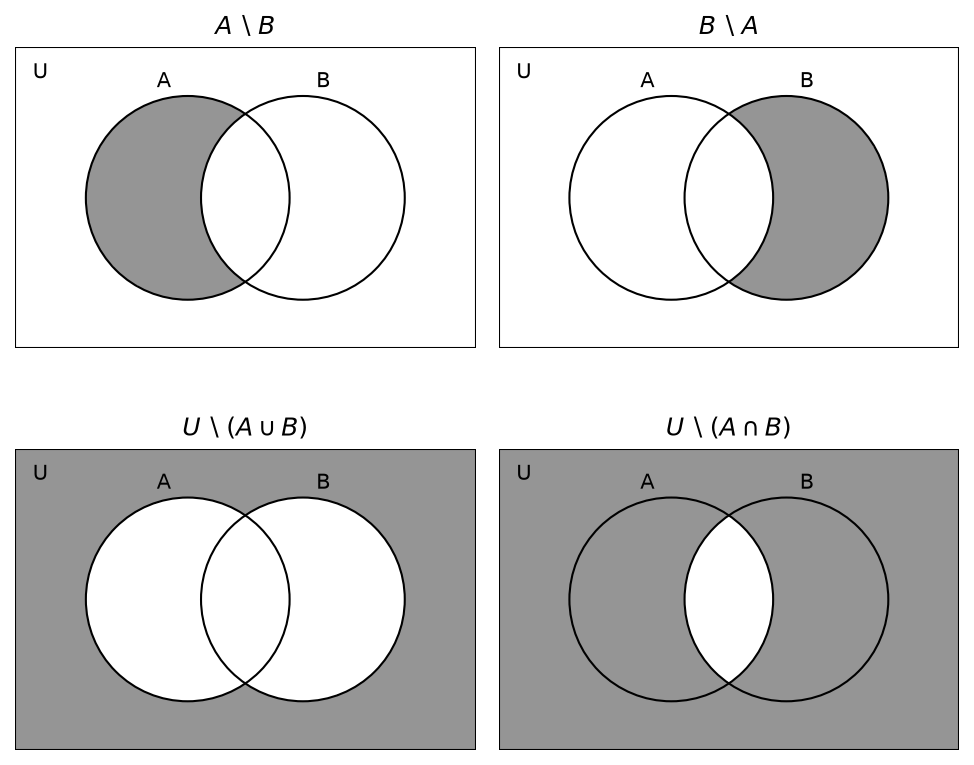
\includegraphics[width=.84\linewidth,height=.38\textheight,keepaspectratio]{figures/C01-HW013-13.png}\end{center}
{\small \field{关联知识}{S04 交集、并集及解集的联系（教材帮p.19、20 / PDF28、29）；S05 全集、补集与德摩根律（教材帮p.21 / PDF30）}
\field{方法与易错点}{先各自化简集合或解出约束，再在数轴上合并；有序数对交集通过联立方程求得。 易错：并集重复写元素；连接处一个闭端点也误删；把交集当并集。}
\field{答案依据}{答案册相关题组：PDF第4、5页（册内页3、4）；按当前题库原题逐项重算，不按旧版题号机械对套。}}

\itemhead{习题1.1 · 第14题（教材p.13）}{XJ-B1-C01-HW-P013-Y1051}
\label{XJ-B1-C01-HW-P013-Y1051}
{\footnotesize 湘教版教材p.13 / PDF第20页 / 习题1.1 / 第14题}
\field{原题}{一家市场调查公司为了了解当地市民在阅读某种报纸（纸质版和电子版）方面的取向，抽样调查了 500 个市民，调查结果显示：订阅纸质版的有 334 人，订阅电子版的有 297 人，其中两种都订的有 150 人。试问：
\subq{1}只订纸质版不订电子版的有多少人？
\subq{2}只订电子版不订纸质版的有多少人？
\subq{3}至少订一种的有多少人？
\subq{4}一种都没订的有多少人？}
\field{参考答案}{（1）184人；（2）147人；（3）481人；（4）19人。并集人数为 $334+297-150$。}
{\small \field{关联知识}{S06 Venn图、容斥与实际计数（教材帮p.22 / PDF31）}
\field{方法与易错点}{先画互不重叠区域，从最内层填写人数，再依据总人数或非负限制求解。 易错：把只参加两项的人数当作完整交集；重复计算三重交集；忽略一种都不参加。}
\field{答案依据}{答案册相关题组：PDF第4、5页（册内页3、4）；按当前题库原题逐项重算，不按旧版题号机械对套。}}

\itemhead{习题1.1 · 第15题（教材p.13）}{XJ-B1-C01-HW-P013-Y1352}
\label{XJ-B1-C01-HW-P013-Y1352}
{\footnotesize 湘教版教材p.13 / PDF第20页 / 习题1.1 / 第15题}
\field{原题}{设 $I=\{x\in\mathbb Z\mid x^3\in[-125,125]\}$，$A=\{2k\mid-5<2k<5,\ k\in\mathbb Z\}$，$B=\{2k+1\mid k\in[0,3),\ k\in\mathbb Z\}$，求 $\complement_I A$，$\complement_I B$。}
\field{参考答案}{$I=\{-5,-4,\ldots,5\},A=\{-4,-2,0,2,4\},B=\{1,3,5\}$。故 $\complement_I A=\{-5,-3,-1,1,3,5\}$；$\complement_I B=\{-5,-4,-3,-2,-1,0,2,4\}$。答案册对应旧题的 $B$ 含负奇数，本题不能沿用。}
\field{核对说明}{版本条件变化：答案册PDF5中的B含负奇数；现教材k\ensuremath{\in}[0,3)，B=\{1,3,5\}，补集相应变化。}
{\small \field{关联知识}{S05 全集、补集与德摩根律（教材帮p.21 / PDF30）}
\field{方法与易错点}{标出全集内的已知集合，取剩余区域，先算括号内部再补集。 易错：忘记全集范围；对“且”的否定仍写“且”；漏闭端点。}
\field{答案依据}{答案册相关题组：PDF第4、5页（册内页3、4）；按当前题库原题逐项重算，不按旧版题号机械对套。}}

\itemhead{习题1.1 · 第16题（教材p.13）}{XJ-B1-C01-HW-P013-Y1442}
\label{XJ-B1-C01-HW-P013-Y1442}
{\footnotesize 湘教版教材p.13 / PDF第20页 / 习题1.1 / 第16题}
\field{原题}{设 $\mathbb R$ 为全集，$A=\{x\mid x<a\}$，$B=\{x\mid1<x<2\}$，且 $A\cup\overline B=\mathbb R$，求 $a$ 的取值范围。}
\field{参考答案}{$a\ge2$。条件等价于 $B\subseteq A$；$B$ 不含端点2，因此 $a=2$ 可以取到。}
{\small \field{关联知识}{S04 交集、并集及解集的联系（教材帮p.19、20 / PDF28、29）；S05 全集、补集与德摩根律（教材帮p.21 / PDF30）}
\field{方法与易错点}{先各自化简集合或解出约束，再在数轴上合并；有序数对交集通过联立方程求得。 易错：并集重复写元素；连接处一个闭端点也误删；把交集当并集。}
\field{答案依据}{答案册相关题组：PDF第4、5页（册内页3、4）；按当前题库原题逐项重算，不按旧版题号机械对套。}}

\itemhead{习题1.1 · 第17题（教材p.13）}{XJ-B1-C01-HW-P013-Y1531}
\label{XJ-B1-C01-HW-P013-Y1531}
{\footnotesize 湘教版教材p.13 / PDF第20页 / 习题1.1 / 第17题}
\field{原题}{已知 $U=\{1,2,3,4,5,6,7,8\}$，$A\cap(\complement_U B)=\{1,8\}$，$(\complement_U A)\cap B=\{2,6\}$，$(\complement_U A)\cap(\complement_U B)=\{4,7\}$，求集合 $A$，$B$。}
\field{参考答案}{$A=\{1,3,5,8\}$，$B=\{2,3,5,6\}$；尚未落入三个已知区域的3、5必须同属 $A\cap B$。}
{\small \field{关联知识}{S05 全集、补集与德摩根律（教材帮p.21 / PDF30）；S06 Venn图、容斥与实际计数（教材帮p.22 / PDF31）}
\field{方法与易错点}{标出全集内的已知集合，取剩余区域，先算括号内部再补集。 易错：忘记全集范围；对“且”的否定仍写“且”；漏闭端点。}
\field{答案依据}{答案册相关题组：PDF第4、5页（册内页3、4）；按当前题库原题逐项重算，不按旧版题号机械对套。}}

\itemhead{1.2 思考 · 未编号题组（教材p.14）}{XJ-B1-C01-TH-P014-Y1066}
\label{XJ-B1-C01-TH-P014-Y1066}
{\footnotesize 湘教版教材p.14 / PDF第21页 / 1.2 思考 / 未编号题组}
\field{原题}{在初中，我们已经对命题有了初步认识。你能说出命题的定义并列举出一些数学中的命题吗？}
\field{参考答案}{命题是可以判断真假的陈述句。例如“2是偶数”为真命题，“1是偶数”为假命题；未限定 $x$ 的“$x>0$”不是命题。}
{\small \field{关联知识}{L01 命题、真假、逆命题与否定（教材帮p.30 / PDF39）}
\field{方法与易错点}{明确论域与断言；真命题给理由，假命题给满足题设而使结论失败的反例。 易错：把逆命题当成否定；只改变结论中的个别词而改变原逻辑范围。}
\field{答案依据}{答案册未提供本栏目的独立对应答案；依据原题、教材概念补写参考回应。开放性总结不设唯一数值答案。}}

\itemhead{1.2 例题 · 例题1（教材p.15）}{XJ-B1-C01-EX-P015-Y0177}
\label{XJ-B1-C01-EX-P015-Y0177}
{\footnotesize 湘教版教材p.15 / PDF第22页 / 1.2 例题 / 例题1}
\field{原题}{下列语句是命题吗？若是，则判断是真命题还是假命题。
\subq{1}$x>0$；
\subq{2}若 $a,b$ 是任意实数且 $a^2>b^2$，则 $a>b$。}
\field{参考答案}{（1）未限定 $x$，不是命题；（2）假命题，例如 $a=-2,b=1$。}
{\small \field{关联知识}{L01 命题、真假、逆命题与否定（教材帮p.30 / PDF39）}
\field{方法与易错点}{明确论域与断言；真命题给理由，假命题给满足题设而使结论失败的反例。 易错：把逆命题当成否定；只改变结论中的个别词而改变原逻辑范围。}
\field{答案依据}{例题原解位置：湘教版教材p.15及题库原图；独立编写可编辑参考解答。答案册此部分主要收练习、习题，不伪造例题答案册位置。}}

\itemhead{1.2 例题 · 例题2（教材p.15）}{XJ-B1-C01-EX-P015-Y0738}
\label{XJ-B1-C01-EX-P015-Y0738}
{\footnotesize 湘教版教材p.15 / PDF第22页 / 1.2 例题 / 例题2}
\field{原题}{写出下列命题 $p$ 的否定 $\neg p$：
\subq{1}$p$：4 是方程 $x^2-16=0$ 的根；
\subq{2}$p$：相似三角形的面积一定相等；
\subq{3}$p$：16 是 4 的倍数。}
\field{参考答案}{（1）4不是方程 $x^2-16=0$ 的根；（2）存在面积不相等的相似三角形；（3）16不是4的倍数。}
{\small \field{关联知识}{L01 命题、真假、逆命题与否定（教材帮p.30 / PDF39）}
\field{方法与易错点}{明确论域与断言；真命题给理由，假命题给满足题设而使结论失败的反例。 易错：把逆命题当成否定；只改变结论中的个别词而改变原逻辑范围。}
\field{答案依据}{例题原解位置：湘教版教材p.15及题库原图；独立编写可编辑参考解答。答案册此部分主要收练习、习题，不伪造例题答案册位置。}}

\itemhead{p.16 练习 · 第1题（教材p.16）}{XJ-B1-C01-PR-P016-Y0217}
\label{XJ-B1-C01-PR-P016-Y0217}
{\footnotesize 湘教版教材p.16 / PDF第23页 / p.16 练习 / 第1题}
\field{原题}{判断下列命题的真假，并说明理由：
\subq{1}若 $a,b$ 是任意实数，则 $|a|+|b|>0$；
\subq{2}若 $x,y$ 是实数且 $x^2+y^2=0$，则 $x=y=0$；
\subq{3}若 $m>0$，则 $x^2+x-m=0$ 有两个不相等的实数根；
\subq{4}若 $x^2+x-m=0$ 有两个不相等的实数根，则实数 $m>0$。}
\field{参考答案}{依次为假、真、真、假。（1）取 $a=b=0$；（2）两个非负数之和为0则都为0；（3）$\Delta=1+4m>0$；（4）反例 $m=0$。}
{\small \field{关联知识}{L01 命题、真假、逆命题与否定（教材帮p.30 / PDF39）；Q01 二次函数、零点、判别式与根系关系（教材帮p.65 / PDF74）}
\field{方法与易错点}{明确论域与断言；真命题给理由，假命题给满足题设而使结论失败的反例。 易错：把逆命题当成否定；只改变结论中的个别词而改变原逻辑范围。}
\field{答案依据}{答案册相关题组：PDF第6页（册内页5）；按当前题库原题逐项重算，不按旧版题号机械对套。}}

\itemhead{p.16 练习 · 第2题（教材p.16）}{XJ-B1-C01-PR-P016-Y0429}
\label{XJ-B1-C01-PR-P016-Y0429}
{\footnotesize 湘教版教材p.16 / PDF第23页 / p.16 练习 / 第2题}
\field{原题}{写出下列命题的否定，并判断其真假。
\subq{1}$p$：5 不是 75 的约数；
\subq{2}$p$：$x>2$ 是不等式 $3x-6>0$ 的解；
\subq{3}$p$：方程 $x^2-2x+3=0$ 有实数根；
\subq{4}$p$：空集是集合 $A$ 的子集。}
\field{参考答案}{（1）5是75的约数，真；（2）$x>2$ 不是该不等式的解，假；（3）方程无实数根，真；（4）空集不是 $A$ 的子集，假。}
{\small \field{关联知识}{L01 命题、真假、逆命题与否定（教材帮p.30 / PDF39）}
\field{方法与易错点}{明确论域与断言；真命题给理由，假命题给满足题设而使结论失败的反例。 易错：把逆命题当成否定；只改变结论中的个别词而改变原逻辑范围。}
\field{答案依据}{答案册相关题组：PDF第6页（册内页5）；按当前题库原题逐项重算，不按旧版题号机械对套。}}

\itemhead{p.16 练习 · 第3题（教材p.16）}{XJ-B1-C01-PR-P016-Y0642}
\label{XJ-B1-C01-PR-P016-Y0642}
{\footnotesize 湘教版教材p.16 / PDF第23页 / p.16 练习 / 第3题}
\field{原题}{写出命题“四边形 $ABCD$ 中，若 $AC\perp BD$，则四边形 $ABCD$ 为菱形”的逆命题。}
\field{参考答案}{逆命题为：若四边形 $ABCD$ 为菱形，则 $AC\perp BD$。这是一个真命题；不要把原命题的真假当作逆命题的真假。}
\field{核对说明}{版本小问变化：答案册PDF6只写“假命题”；现题要求写逆命题，逆命题为真，不能照抄。}
{\small \field{关联知识}{L01 命题、真假、逆命题与否定（教材帮p.30 / PDF39）}
\field{方法与易错点}{明确论域与断言；真命题给理由，假命题给满足题设而使结论失败的反例。 易错：把逆命题当成否定；只改变结论中的个别词而改变原逻辑范围。}
\field{答案依据}{答案册相关题组：PDF第6页（册内页5）；按当前题库原题逐项重算，不按旧版题号机械对套。}}

\itemhead{1.2 思考 · 未编号题组（教材p.16）}{XJ-B1-C01-TH-P016-Y0927}
\label{XJ-B1-C01-TH-P016-Y0927}
{\footnotesize 湘教版教材p.16 / PDF第23页 / 1.2 思考 / 未编号题组}
\field{原题}{对于 1.2.1 小节例 2 后面列出的 6 个命题，哪些是真命题？哪些是假命题？
\par\textit{所引用的教材 p.15 六个命题如下：}
\subq{1}若两个三角形全等，则它们相似；
\subq{2}若两个三角形相似，则它们全等；
\subq{3}若实数 $a\ne0$，则 $a^2>0$；
\subq{4}若四边形 $ABCD$ 为菱形，则 $AC\perp BD$；
\subq{5}若 $a<0$，则方程 $ax^2+4x-3=0$ 没有正的实根；
\subq{6}若 $a=b$，则 $a^2=b^2$。}
\field{参考答案}{依次为真、假、真、真、假、真。（2）反例为大小不同的等边三角形；（5）取 $a=-1$，方程有正根1、3。}
{\small \field{关联知识}{L01 命题、真假、逆命题与否定（教材帮p.30 / PDF39）}
\field{方法与易错点}{明确论域与断言；真命题给理由，假命题给满足题设而使结论失败的反例。 易错：把逆命题当成否定；只改变结论中的个别词而改变原逻辑范围。}
\field{答案依据}{答案册未提供本栏目的独立对应答案；依据原题、教材概念补写参考回应。开放性总结不设唯一数值答案。}}

\itemhead{1.2 例题 · 例题3（教材p.17）}{XJ-B1-C01-EX-P017-Y0928}
\label{XJ-B1-C01-EX-P017-Y0928}
{\footnotesize 湘教版教材p.17 / PDF第24页 / 1.2 例题 / 例题3}
\field{原题}{判断下列结论是否成立，并说明理由。
\subq{1}$p$：$x^2=1$，$q$：$x=1$，$p$ 是 $q$ 的充分条件；
\subq{2}$p$：四边形的对角线互相垂直，$q$：四边形是菱形，$q$ 是 $p$ 的必要条件；
\subq{3}$p$：$xy>0$，$q$：$x>0,\ y>0$，$p$ 是 $q$ 的充要条件。}
\field{参考答案}{三项结论都不成立。（1）$x=-1$；（2）对角线垂直不必为菱形；（3）$x=y=-1$ 说明 $p$ 不能推出 $q$。}
{\small \field{关联知识}{L02 充分、必要、充要条件（教材帮p.30、31 / PDF39、40）}
\field{方法与易错点}{分别检查两个方向；用解集包含或具体反例判定，不凭句子位置猜方向。 易错：把“必要”箭头反写；只有一个方向证据便断言“不必要”；忽略给定论域。}
\field{答案依据}{例题原解位置：湘教版教材p.17及题库原图；独立编写可编辑参考解答。答案册此部分主要收练习、习题，不伪造例题答案册位置。}}

\itemhead{1.2 例题 · 例题4（教材p.17）}{XJ-B1-C01-EX-P017-Y1338}
\label{XJ-B1-C01-EX-P017-Y1338}
{\footnotesize 湘教版教材p.17 / PDF第24页 / 1.2 例题 / 例题4}
\field{原题}{从“充分而不必要条件”“必要而不充分条件”“充要条件”和“既不充分又不必要条件”中选择适当的一种填空。
\subq{1}$a\ge5$ 是 $a$ 为正数的\blank；
\subq{2}四边形的两对角线相等是该四边形为矩形的\blank；
\subq{3}四边形的一组对边平行且相等是四边形的两组对边分别平行的\blank；
\subq{4}若 $x\in\mathbb R$，则 $x^2=2$ 是 $x=2$ 的\blank。}
\field{参考答案}{依次为充分而不必要、必要而不充分、充要、既不充分又不必要条件。}
{\small \field{关联知识}{L02 充分、必要、充要条件（教材帮p.30、31 / PDF39、40）}
\field{方法与易错点}{分别检查两个方向；用解集包含或具体反例判定，不凭句子位置猜方向。 易错：把“必要”箭头反写；只有一个方向证据便断言“不必要”；忽略给定论域。}
\field{答案依据}{例题原解位置：湘教版教材p.17及题库原图；独立编写可编辑参考解答。答案册此部分主要收练习、习题，不伪造例题答案册位置。}}

\itemhead{1.2 例题 · 例题5（教材p.18）}{XJ-B1-C01-EX-P018-Y0491}
\label{XJ-B1-C01-EX-P018-Y0491}
{\footnotesize 湘教版教材p.18 / PDF第25页 / 1.2 例题 / 例题5}
\field{原题}{试证：
\subq{1}在实数范围内，$x=1$ 是 $x^2=1$ 的充分而不必要条件；
\subq{2}四边形的两组对边分别相等是四边形为矩形的必要而不充分条件；
\subq{3}在 $\triangle ABC$ 中，$\angle B=\angle C$ 是 $AC=AB$ 的充要条件。}
\field{参考答案}{（1）$x=1\Rightarrow x^2=1$，反向有反例 $x=-1$；（2）矩形对边分别相等，斜的平行四边形说明反向不成立；（3）利用等边对等角和等角对等边双向推出。}
{\small \field{关联知识}{L02 充分、必要、充要条件（教材帮p.30、31 / PDF39、40）}
\field{方法与易错点}{分别检查两个方向；用解集包含或具体反例判定，不凭句子位置猜方向。 易错：把“必要”箭头反写；只有一个方向证据便断言“不必要”；忽略给定论域。}
\field{答案依据}{例题原解位置：湘教版教材p.18及题库原图；独立编写可编辑参考解答。答案册此部分主要收练习、习题，不伪造例题答案册位置。}}

\itemhead{p.19 练习 · 第1题（教材p.19）}{XJ-B1-C01-PR-P019-Y0218}
\label{XJ-B1-C01-PR-P019-Y0218}
{\footnotesize 湘教版教材p.19 / PDF第26页 / p.19 练习 / 第1题}
\field{原题}{判断下列结论是否成立，并说明理由。
\subq{1}$p$：四边形有三个内角都为直角，$q$：四边形是矩形，$p$ 是 $q$ 的充分条件；
\subq{2}设 $x,y\in\mathbb R$，$p$：$x^2+y^2\ne0$，$q$：$xy\ne0$，$q$ 是 $p$ 的必要条件；
\subq{3}$p$：$x>0,\ y>0$，$q$：$xy>0$，$p$ 是 $q$ 的充要条件。}
\field{参考答案}{（1）成立；（2）不成立，取 $x=1,y=0$，$p$ 成立而 $q$ 不成立；（3）不成立，$x=y=-1$ 是反例。}
{\small \field{关联知识}{L02 充分、必要、充要条件（教材帮p.30、31 / PDF39、40）}
\field{方法与易错点}{分别检查两个方向；用解集包含或具体反例判定，不凭句子位置猜方向。 易错：把“必要”箭头反写；只有一个方向证据便断言“不必要”；忽略给定论域。}
\field{答案依据}{答案册相关题组：PDF第6页（册内页5）；按当前题库原题逐项重算，不按旧版题号机械对套。}}

\itemhead{p.19 练习 · 第2题（教材p.19）}{XJ-B1-C01-PR-P019-Y0389}
\label{XJ-B1-C01-PR-P019-Y0389}
{\footnotesize 湘教版教材p.19 / PDF第26页 / p.19 练习 / 第2题}
\field{原题}{从“充分而不必要条件”“必要而不充分条件”“充要条件”与“既不充分又不必要条件”中选出适当的一种填空：
\subq{1}$\triangle ABC$ 中，$\angle C=90^\circ$ 是 $AB^2=AC^2+BC^2$ 的\blank；
\subq{2}$x>0$ 是 $x\ge1$ 的\blank；
\subq{3}$x=2$ 是 $x^2=4$ 的\blank；
\subq{4}$0<x<2$ 是 $1<x<3$ 的\blank。}
\field{参考答案}{依次为充要、必要而不充分、充分而不必要、既不充分又不必要条件。}
{\small \field{关联知识}{L02 充分、必要、充要条件（教材帮p.30、31 / PDF39、40）}
\field{方法与易错点}{分别检查两个方向；用解集包含或具体反例判定，不凭句子位置猜方向。 易错：把“必要”箭头反写；只有一个方向证据便断言“不必要”；忽略给定论域。}
\field{答案依据}{答案册相关题组：PDF第6页（册内页5）；按当前题库原题逐项重算，不按旧版题号机械对套。}}

\itemhead{p.19 练习 · 第3题（教材p.19）}{XJ-B1-C01-PR-P019-Y0648}
\label{XJ-B1-C01-PR-P019-Y0648}
{\footnotesize 湘教版教材p.19 / PDF第26页 / p.19 练习 / 第3题}
\field{原题}{已知 $m\in\mathbb R$，集合 $M=\{1,3,m+2\}$，$N=\{0,6\}$。求证：“$m=4$”是“$M\cap N=\{6\}$”的充要条件。}
\field{参考答案}{$m=4$ 时 $M=\{1,3,6\}$，交集为 $\{6\}$；反之6只能来自 $m+2$，故 $m=4$。两个方向均成立。}
{\small \field{关联知识}{L02 充分、必要、充要条件（教材帮p.30、31 / PDF39、40）；S04 交集、并集及解集的联系（教材帮p.19、20 / PDF28、29）}
\field{方法与易错点}{分别检查两个方向；用解集包含或具体反例判定，不凭句子位置猜方向。 易错：把“必要”箭头反写；只有一个方向证据便断言“不必要”；忽略给定论域。}
\field{答案依据}{答案册相关题组：PDF第6页（册内页5）；按当前题库原题逐项重算，不按旧版题号机械对套。}}

\itemhead{1.2 思考 · 未编号题组（教材p.19）}{XJ-B1-C01-TH-P019-Y1033}
\label{XJ-B1-C01-TH-P019-Y1033}
{\footnotesize 湘教版教材p.19 / PDF第26页 / 1.2 思考 / 未编号题组}
\field{原题}{下列语句是命题吗？将（2）（3）分别与（1）比较，你发现了什么？
\subq{1}$x>0$；
\subq{2}对每一个实数 $x$，有 $x>0$；
\subq{3}有一个实数 $x$，使 $x>0$。}
\field{参考答案}{（1）不是命题；（2）（3）都是命题，前者是假命题，后者是真命题。量词限定了变量的范围及断言方式。}
{\small \field{关联知识}{L03 全称、存在量词及真假的判定（教材帮p.38、39 / PDF47、48）}
\field{方法与易错点}{先确认量词、作用对象及论域，再采用任意性证明或实例反例。 易错：用几个满足的数证明全称命题；把“存在”理解为“唯一存在”。}
\field{答案依据}{答案册未提供本栏目的独立对应答案；依据原题、教材概念补写参考回应。开放性总结不设唯一数值答案。}}

\itemhead{1.2 例题 · 例题6（教材p.20）}{XJ-B1-C01-EX-P020-Y0562}
\label{XJ-B1-C01-EX-P020-Y0562}
{\footnotesize 湘教版教材p.20 / PDF第27页 / 1.2 例题 / 例题6}
\field{原题}{指出下列命题中使用了什么量词以及量词的作用范围，并把量词用相应的数学符号取代：
\subq{1}对任意正实数 $a$，$a^2-a-2>0$；
\subq{2}对某个大于 10 的正整数 $n$，$(\sqrt2)^n=1024$。}
\field{参考答案}{（1）全称量词，范围为 $\mathbb R_+$，写作 $\forall a\in\mathbb R_+,a^2-a-2>0$；（2）存在量词，范围为大于10的正整数，写作 $\exists n\in\mathbb Z_+,n>10,(\sqrt2)^n=1024$。}
{\small \field{关联知识}{L03 全称、存在量词及真假的判定（教材帮p.38、39 / PDF47、48）}
\field{方法与易错点}{先确认量词、作用对象及论域，再采用任意性证明或实例反例。 易错：用几个满足的数证明全称命题；把“存在”理解为“唯一存在”。}
\field{答案依据}{例题原解位置：湘教版教材p.20及题库原图；独立编写可编辑参考解答。答案册此部分主要收练习、习题，不伪造例题答案册位置。}}

\itemhead{1.2 思考 · 未编号题组（教材p.20）}{XJ-B1-C01-TH-P020-Y0942}
\label{XJ-B1-C01-TH-P020-Y0942}
{\footnotesize 湘教版教材p.20 / PDF第27页 / 1.2 思考 / 未编号题组}
\field{原题}{如何判断全称量词命题的真假？如何判断存在量词命题的真假？}
\field{参考答案}{全称命题真须对范围内每一个对象证明，假只需一个反例；存在命题真只需给出一个对象，假须证明范围内所有对象均不满足。}
{\small \field{关联知识}{L03 全称、存在量词及真假的判定（教材帮p.38、39 / PDF47、48）}
\field{方法与易错点}{先确认量词、作用对象及论域，再采用任意性证明或实例反例。 易错：用几个满足的数证明全称命题；把“存在”理解为“唯一存在”。}
\field{答案依据}{答案册未提供本栏目的独立对应答案；依据原题、教材概念补写参考回应。开放性总结不设唯一数值答案。}}

\itemhead{1.2 例题 · 例题7（教材p.20）}{XJ-B1-C01-EX-P020-Y1143}
\label{XJ-B1-C01-EX-P020-Y1143}
{\footnotesize 湘教版教材p.20 / PDF第27页 / 1.2 例题 / 例题7}
\field{原题}{判断下列全称量词命题的真假：
\subq{1}$\forall x\in\mathbb R,\ x^2+2>0$；
\subq{2}$\forall x\in\mathbb N,\ x^4\ge1$。}
\field{参考答案}{（1）真，$x^2+2\ge2>0$；（2）假，$0\in\mathbb N$ 且 $0^4<1$。}
{\small \field{关联知识}{L03 全称、存在量词及真假的判定（教材帮p.38、39 / PDF47、48）}
\field{方法与易错点}{先确认量词、作用对象及论域，再采用任意性证明或实例反例。 易错：用几个满足的数证明全称命题；把“存在”理解为“唯一存在”。}
\field{答案依据}{例题原解位置：湘教版教材p.20及题库原图；独立编写可编辑参考解答。答案册此部分主要收练习、习题，不伪造例题答案册位置。}}

\itemhead{1.2 例题 · 例题8（教材p.21）}{XJ-B1-C01-EX-P021-Y0177}
\label{XJ-B1-C01-EX-P021-Y0177}
{\footnotesize 湘教版教材p.21 / PDF第28页 / 1.2 例题 / 例题8}
\field{原题}{判断下列存在量词命题的真假：
\subq{1}$\exists a\in\mathbb Z,\ a^2=3a-2$；
\subq{2}$\exists a\ge3,\ a^2=3a-2$；
\subq{3}设 $A,B,C$ 是平面上不在同一直线上的三点，在该平面上存在某个点 $P$，使得 $PA=PB=PC$。}
\field{参考答案}{（1）真，$a=1$ 或2；（2）假，方程仅有根1、2；（3）真，三角形三边垂直平分线的交点即外心。}
{\small \field{关联知识}{L03 全称、存在量词及真假的判定（教材帮p.38、39 / PDF47、48）}
\field{方法与易错点}{先确认量词、作用对象及论域，再采用任意性证明或实例反例。 易错：用几个满足的数证明全称命题；把“存在”理解为“唯一存在”。}
\field{答案依据}{例题原解位置：湘教版教材p.21及题库原图；独立编写可编辑参考解答。答案册此部分主要收练习、习题，不伪造例题答案册位置。}}

\itemhead{p.21 练习 · 第1题（教材p.21）}{XJ-B1-C01-PR-P021-Y0793}
\label{XJ-B1-C01-PR-P021-Y0793}
{\footnotesize 湘教版教材p.21 / PDF第28页 / p.21 练习 / 第1题}
\field{原题}{指出下列命题中使用了什么量词以及量词的作用范围，并把量词用相应的数学符号取代：
\subq{1}对任意整数 $n$，$2n+1$ 是奇数；
\subq{2}对某个有理数 $x$，有 $4x=\dfrac12$；
\subq{3}线段 $AB$ 上有一点 $M$ 满足比例式 $\dfrac{AM}{MB}=\dfrac{MB}{AB}$。}
\field{参考答案}{（1）全称，$\forall n\in\mathbb Z,2n+1$ 为奇数；（2）存在，$\exists x\in\mathbb Q,4x=\frac12$；（3）存在，$\exists M\in\overline{AB}$，满足 $MB\ne0$ 且 $AM/MB=MB/AB$。}
{\small \field{关联知识}{L03 全称、存在量词及真假的判定（教材帮p.38、39 / PDF47、48）}
\field{方法与易错点}{先确认量词、作用对象及论域，再采用任意性证明或实例反例。 易错：用几个满足的数证明全称命题；把“存在”理解为“唯一存在”。}
\field{答案依据}{答案册相关题组：PDF第6页（册内页5）；按当前题库原题逐项重算，不按旧版题号机械对套。}}

\itemhead{p.21 练习 · 第2题（教材p.21）}{XJ-B1-C01-PR-P021-Y1067}
\label{XJ-B1-C01-PR-P021-Y1067}
{\footnotesize 湘教版教材p.21 / PDF第28页 / p.21 练习 / 第2题}
\field{原题}{判断下列命题的真假：
\subq{1}$\exists x\in\mathbb Z,\ x^2=2$；
\subq{2}$\exists x\in\mathbb R,\ x^2=2$；
\subq{3}线段的垂直平分线上的点到这条线段两个端点的距离相等；
\subq{4}平面上任意两条直线必有交点。}
\field{参考答案}{依次为假、真、真、假。反例分别可用整数平方不能等于2、平面内两条不同的平行直线。}
{\small \field{关联知识}{L03 全称、存在量词及真假的判定（教材帮p.38、39 / PDF47、48）}
\field{方法与易错点}{先确认量词、作用对象及论域，再采用任意性证明或实例反例。 易错：用几个满足的数证明全称命题；把“存在”理解为“唯一存在”。}
\field{答案依据}{答案册相关题组：PDF第6页（册内页5）；按当前题库原题逐项重算，不按旧版题号机械对套。}}

\itemhead{1.2 思考 · 未编号题组（教材p.21）}{XJ-B1-C01-TH-P021-Y1462}
\label{XJ-B1-C01-TH-P021-Y1462}
{\footnotesize 湘教版教材p.21 / PDF第28页 / 1.2 思考 / 未编号题组}
\field{原题}{前面学习了命题的否定，对含有量词的命题如何进行否定呢？}
\field{参考答案}{保留原论域，交换 $\forall$ 与 $\exists$，并否定断言：$\neg(\forall x\in M,p(x))\Leftrightarrow\exists x\in M,\neg p(x)$；存在命题的否定同理。}
{\small \field{关联知识}{L04 含一个量词命题的否定（教材帮p.39、40 / PDF48、49）}
\field{方法与易错点}{分三步书写：保留论域、交换量词、否定断言，再判断新命题真假。 易错：只改量词不改结论；把不等号否定成反向但遗漏等号。}
\field{答案依据}{答案册未提供本栏目的独立对应答案；依据原题、教材概念补写参考回应。开放性总结不设唯一数值答案。}}

\itemhead{1.2 例题 · 例题9（教材p.22）}{XJ-B1-C01-EX-P022-Y0891}
\label{XJ-B1-C01-EX-P022-Y0891}
{\footnotesize 湘教版教材p.22 / PDF第29页 / 1.2 例题 / 例题9}
\field{原题}{写出下列含量词命题的否定：
\subq{1}$p$：所有二次函数的图象都是轴对称图形；
\subq{2}$q$：$\exists x\in\mathbb R,\ -2x^2+4x-3>0$；
\subq{3}$r$：三角形的垂心都在其外部；
\subq{4}$s$：有一个小于 210 的正整数至少有 4 个质因数。}
\field{参考答案}{（1）存在一个二次函数，其图象不是轴对称图形；（2）$\forall x\in\mathbb R,-2x^2+4x-3\le0$；（3）存在一个三角形，其垂心不在外部；（4）每一个小于210的正整数的质因数都少于4个。}
{\small \field{关联知识}{L04 含一个量词命题的否定（教材帮p.39、40 / PDF48、49）}
\field{方法与易错点}{分三步书写：保留论域、交换量词、否定断言，再判断新命题真假。 易错：只改量词不改结论；把不等号否定成反向但遗漏等号。}
\field{答案依据}{例题原解位置：湘教版教材p.22及题库原图；独立编写可编辑参考解答。答案册此部分主要收练习、习题，不伪造例题答案册位置。}}

\itemhead{1.2 例题 · 例题10（教材p.22）}{XJ-B1-C01-EX-P022-Y1296}
\label{XJ-B1-C01-EX-P022-Y1296}
{\footnotesize 湘教版教材p.22 / PDF第29页 / 1.2 例题 / 例题10}
\field{原题}{对下列含有量词的命题作否定，并判断其真假：
\subq{1}$p$：任意正实数都有算术平方根；
\subq{2}$q$：$\exists x\in\mathbb R,\ x^2+3\le0$。}
\field{参考答案}{（1）存在一个没有算术平方根的正实数，假；（2）$\forall x\in\mathbb R,x^2+3>0$，真。}
{\small \field{关联知识}{L04 含一个量词命题的否定（教材帮p.39、40 / PDF48、49）}
\field{方法与易错点}{分三步书写：保留论域、交换量词、否定断言，再判断新命题真假。 易错：只改量词不改结论；把不等号否定成反向但遗漏等号。}
\field{答案依据}{例题原解位置：湘教版教材p.22及题库原图；独立编写可编辑参考解答。答案册此部分主要收练习、习题，不伪造例题答案册位置。}}

\itemhead{p.23 练习 · 未编号题组（教材p.23）}{XJ-B1-C01-PR-P023-Y0176}
\label{XJ-B1-C01-PR-P023-Y0176}
{\footnotesize 湘教版教材p.23 / PDF第30页 / p.23 练习 / 未编号题组}
\field{原题}{对下列含有量词的命题作否定，并判断其真假：
\subq{1}$\forall x\in\mathbb R,\ x^2-2x+1\ge0$；
\subq{2}$\exists x\in\mathbb Q,\ x^2=2$；
\subq{3}$\exists x\in\mathbb R,\ x^2-3=0$；
\subq{4}$\forall x\ne0,\ \left(x+\dfrac1x\right)\in[2,+\infty)$；
\subq{5}任意三角形都有内切圆；
\subq{6}任意两个直角三角形都是相似三角形。}
\field{参考答案}{依次为：（1）$\exists x\in\mathbb R,(x-1)^2<0$，假；（2）$\forall x\in\mathbb Q,x^2\ne2$，真；（3）$\forall x\in\mathbb R,x^2-3\ne0$，假；（4）$\exists x\ne0,x+1/x\notin[2,+\infty)$，真（取 $x=-1$）；（5）存在没有内切圆的三角形，假；（6）存在不相似的两个直角三角形，真。}
{\small \field{关联知识}{L04 含一个量词命题的否定（教材帮p.39、40 / PDF48、49）}
\field{方法与易错点}{分三步书写：保留论域、交换量词、否定断言，再判断新命题真假。 易错：只改量词不改结论；把不等号否定成反向但遗漏等号。}
\field{答案依据}{答案册相关题组：PDF第6、7页（册内页5、6）；按当前题库原题逐项重算，不按旧版题号机械对套。}}

\itemhead{习题1.2 · 第1题（教材p.23）}{XJ-B1-C01-HW-P023-Y0778}
\label{XJ-B1-C01-HW-P023-Y0778}
{\footnotesize 湘教版教材p.23 / PDF第30页 / 习题1.2 / 第1题}
\field{原题}{判断下列命题的真假，并说明理由：
\subq{1}菱形的两条对角线相等；
\subq{2}末位是 5 的整数可以被 5 整除；
\subq{3}$x=5$ 是方程 $x^2-4x-5=0$ 的根；
\subq{4}到圆心的距离等于该圆半径的直线是圆的切线。}
\field{参考答案}{依次为假、真、真、真。（1）非正方形的菱形即反例；（3）代入得0；（4）由圆心到直线距离与半径的判定。}
{\small \field{关联知识}{L01 命题、真假、逆命题与否定（教材帮p.30 / PDF39）}
\field{方法与易错点}{明确论域与断言；真命题给理由，假命题给满足题设而使结论失败的反例。 易错：把逆命题当成否定；只改变结论中的个别词而改变原逻辑范围。}
\field{答案依据}{答案册相关题组：PDF第7页（册内页6）；按当前题库原题逐项重算，不按旧版题号机械对套。}}

\itemhead{习题1.2 · 第2题（教材p.23）}{XJ-B1-C01-HW-P023-Y0993}
\label{XJ-B1-C01-HW-P023-Y0993}
{\footnotesize 湘教版教材p.23 / PDF第30页 / 习题1.2 / 第2题}
\field{原题}{写出下列命题的否定，并判断其真假。
\subq{1}$p$：边长分别为 5，12，13 的三角形是直角三角形；
\subq{2}$q$：面积相等的三角形都是全等三角形；
\subq{3}$s$：二次函数 $y=x^2-2x+3$ 的图象与 $x$ 轴没有交点。}
\field{参考答案}{（1）边长为5、12、13的三角形不是直角三角形，假；（2）存在面积相等但不全等的两个三角形，真；（3）$y=x^2-2x+3$ 的图象与 $x$ 轴有交点，假。答案册此处第三问的题干不同，已按本题重算。}
\field{核对说明}{版本题干变化：答案册PDF7第2题第3问为xy\ensuremath{\ne}0的否定；现教材问二次函数与x轴的交点。}
{\small \field{关联知识}{L01 命题、真假、逆命题与否定（教材帮p.30 / PDF39）；L04 含一个量词命题的否定（教材帮p.39、40 / PDF48、49）}
\field{方法与易错点}{明确论域与断言；真命题给理由，假命题给满足题设而使结论失败的反例。 易错：把逆命题当成否定；只改变结论中的个别词而改变原逻辑范围。}
\field{答案依据}{答案册相关题组：PDF第7页（册内页6）；按当前题库原题逐项重算，不按旧版题号机械对套。}}

\itemhead{习题1.2 · 第3题（教材p.23）}{XJ-B1-C01-HW-P023-Y1165}
\label{XJ-B1-C01-HW-P023-Y1165}
{\footnotesize 湘教版教材p.23 / PDF第30页 / 习题1.2 / 第3题}
\field{原题}{在下列各题中，试判断 $p$ 是否是 $q$ 的充分条件。
\subq{1}设 $a,b\in\mathbb R$，$p$：$ab=0$，$q$：$a^2+b^2=0$；
\subq{2}设 $a,b,c\in\mathbb R$，$p$：$x=1$ 是方程 $ax^2+bx+c=0$ 的一个根，$q$：$a+b+c=0$；
\subq{3}$p$：$A\cap B$ 为空集，$q$：$A$ 与 $B$ 中至少有一个为空集。}
\field{参考答案}{（1）不是，取 $a=0,b=1$；（2）是，代入 $x=1$ 即得；（3）不是，取 $A=\{1\},B=\{2\}$。}
\field{核对说明}{版本题号变化：现教材有独立的充分条件三问，答案册同组题号不能逐号对套。}
{\small \field{关联知识}{L02 充分、必要、充要条件（教材帮p.30、31 / PDF39、40）}
\field{方法与易错点}{分别检查两个方向；用解集包含或具体反例判定，不凭句子位置猜方向。 易错：把“必要”箭头反写；只有一个方向证据便断言“不必要”；忽略给定论域。}
\field{答案依据}{答案册相关题组：PDF第7页（册内页6）；按当前题库原题逐项重算，不按旧版题号机械对套。}}

\itemhead{习题1.2 · 第4题（教材p.23）}{XJ-B1-C01-HW-P023-Y1381}
\label{XJ-B1-C01-HW-P023-Y1381}
{\footnotesize 湘教版教材p.23 / PDF第30页 / 习题1.2 / 第4题}
\field{原题}{判断下列结论是否成立，并说明理由。
\subq{1}$p$：$a>b$，$q$：$ac^2>bc^2$，$p$ 是 $q$ 的充分条件；
\subq{2}$p$：$x^2\ne1$，$q$：$x\ne1$，$p$ 是 $q$ 的必要条件；
\subq{3}$p$：四边形为正方形，$q$：四边形为矩形，$p$ 是 $q$ 的充分而不必要条件；
\subq{4}$p$：$a>b$，$q$：$a+c>b+c$，$p$ 是 $q$ 的充要条件；
\subq{5}$p$：$x\in A\cap B$，$q$：$x\in A$，$p$ 是 $q$ 的充要条件。}
\field{参考答案}{依次为不成立、不成立、成立、成立、不成立。（1）漏 $c\ne0$；（2）$x=-1$ 为反例；（5）$x\in A$ 未必属于 $B$。}
{\small \field{关联知识}{L02 充分、必要、充要条件（教材帮p.30、31 / PDF39、40）}
\field{方法与易错点}{分别检查两个方向；用解集包含或具体反例判定，不凭句子位置猜方向。 易错：把“必要”箭头反写；只有一个方向证据便断言“不必要”；忽略给定论域。}
\field{答案依据}{答案册相关题组：PDF第7页（册内页6）；按当前题库原题逐项重算，不按旧版题号机械对套。}}

\itemhead{习题1.2 · 第5题（教材p.24）}{XJ-B1-C01-HW-P024-Y0260}
\label{XJ-B1-C01-HW-P024-Y0260}
{\footnotesize 湘教版教材p.24 / PDF第31页 / 习题1.2 / 第5题}
\field{原题}{从“充分而不必要条件”“必要而不充分条件”“充要条件”与“既不充分又不必要条件”中选出适当的一种填空：
\subq{1}“$a-1>0$”是“$a>1$”的\blank；
\subq{2}“$a>0,\ b>0$”是“$a+b>1$”的\blank；
\subq{3}“两个角是对顶角”是“两个角相等”的\blank；
\subq{4}设 $a,b,c$ 都是实数，“$ac=bc$”是“$a=b$”的\blank。}
\field{参考答案}{依次为充要、既不充分又不必要、充分而不必要、必要而不充分条件。}
{\small \field{关联知识}{L02 充分、必要、充要条件（教材帮p.30、31 / PDF39、40）}
\field{方法与易错点}{分别检查两个方向；用解集包含或具体反例判定，不凭句子位置猜方向。 易错：把“必要”箭头反写；只有一个方向证据便断言“不必要”；忽略给定论域。}
\field{答案依据}{答案册相关题组：PDF第7页（册内页6）；按当前题库原题逐项重算，不按旧版题号机械对套。}}

\itemhead{习题1.2 · 第6题（教材p.24）}{XJ-B1-C01-HW-P024-Y0518}
\label{XJ-B1-C01-HW-P024-Y0518}
{\footnotesize 湘教版教材p.24 / PDF第31页 / 习题1.2 / 第6题}
\field{原题}{对下列含有量词的命题作否定，并判断其真假：
\subq{1}存在某个整数 $a$，使得 $a^2=a$；
\subq{2}任意实数都可以写成平方和的形式；
\subq{3}每个能被写成两个奇数之和的整数都是偶数；
\subq{4}$\forall m>0$，方程 $x^2+x-m=0$ 有实数根；
\subq{5}$\exists m>0$，方程 $x^2+x+m=0$ 有实数根。}
\field{参考答案}{（1）$\forall a\in\mathbb Z,a^2\ne a$，假；（2）存在不能写成平方和的实数，真（负实数）；（3）存在一个能写成两个奇数之和的整数不是偶数，假；（4）$\exists m>0$，方程 $x^2+x-m=0$ 无实根，假；（5）$\forall m>0$，方程 $x^2+x+m=0$ 无实根，假（取 $m=1/8$）。}
{\small \field{关联知识}{L04 含一个量词命题的否定（教材帮p.39、40 / PDF48、49）}
\field{方法与易错点}{分三步书写：保留论域、交换量词、否定断言，再判断新命题真假。 易错：只改量词不改结论；把不等号否定成反向但遗漏等号。}
\field{答案依据}{答案册相关题组：PDF第7页（册内页6）；按当前题库原题逐项重算，不按旧版题号机械对套。}}

\itemhead{习题1.2 · 第7题（教材p.24）}{XJ-B1-C01-HW-P024-Y0897}
\label{XJ-B1-C01-HW-P024-Y0897}
{\footnotesize 湘教版教材p.24 / PDF第31页 / 习题1.2 / 第7题}
\field{原题}{下列各题中，$p$ 是 $q$ 的什么条件（在“充分而不必要条件”“必要而不充分条件”“充要条件”“既不充分又不必要条件”中选出一种）？为什么？
\subq{1}已知集合 $A=\{1,a\}$，$B=\{1,2,3\}$，$p$：$a=3$，$q$：$A\subseteq B$；
\subq{2}$p$：$a\in\mathbb N_+$，$q$：$a\in\mathbb Z_+$；
\subq{3}设 $x,y$ 是实数，$p$：$x>y$，$q$：$|x|>|y|$；
\subq{4}$p$：$D$ 在 $\triangle ABC$ 的边 $BC$ 的中线上，$q$：$\triangle ABD$ 的面积 $=\triangle ACD$ 的面积。}
\field{参考答案}{依次为充分而不必要、充要、既不充分又不必要、充分而不必要条件。（4）中线上的点必使两面积相等，但中线所在直线上三角形外的点也可使面积相等。}
{\small \field{关联知识}{L02 充分、必要、充要条件（教材帮p.30、31 / PDF39、40）}
\field{方法与易错点}{分别检查两个方向；用解集包含或具体反例判定，不凭句子位置猜方向。 易错：把“必要”箭头反写；只有一个方向证据便断言“不必要”；忽略给定论域。}
\field{答案依据}{答案册相关题组：PDF第7页（册内页6）；按当前题库原题逐项重算，不按旧版题号机械对套。}}

\itemhead{习题1.2 · 第8题（教材p.24）}{XJ-B1-C01-HW-P024-Y1155}
\label{XJ-B1-C01-HW-P024-Y1155}
{\footnotesize 湘教版教材p.24 / PDF第31页 / 习题1.2 / 第8题}
\field{原题}{已知 $p$ 是 $r$ 的充分条件，而 $r$ 是 $q$ 的必要条件，同时也是 $s$ 的充分条件，$q$ 是 $s$ 的必要条件，那么：
\subq{1}$s$ 是 $p$ 的什么条件？
\subq{2}$p$ 是 $q$ 的什么条件？
\subq{3}在 $p,q,r,s$ 中，哪几对互为充要条件？}
\field{参考答案}{由 $p\Rightarrow r$ 及 $q\Rightarrow r\Rightarrow s\Rightarrow q$，得（1）$s$ 是 $p$ 的必要条件；（2）$p$ 是 $q$ 的充分条件；（3）$q,r,s$ 两两互为充要条件。题设不能排除 $p$ 与它们也等价，所以前两问不额外断言“不充分”或“不必要”。}
\field{核对说明}{逻辑强度提醒：题设只推出充分或必要，不能无依据增加“不必要”或“不充分”。}
{\small \field{关联知识}{L02 充分、必要、充要条件（教材帮p.30、31 / PDF39、40）}
\field{方法与易错点}{分别检查两个方向；用解集包含或具体反例判定，不凭句子位置猜方向。 易错：把“必要”箭头反写；只有一个方向证据便断言“不必要”；忽略给定论域。}
\field{答案依据}{答案册相关题组：PDF第7页（册内页6）；按当前题库原题逐项重算，不按旧版题号机械对套。}}

\itemhead{习题1.2 · 第9题（教材p.24）}{XJ-B1-C01-HW-P024-Y1370}
\label{XJ-B1-C01-HW-P024-Y1370}
{\footnotesize 湘教版教材p.24 / PDF第31页 / 习题1.2 / 第9题}
\field{原题}{对下列含有量词的命题作否定，并判断其真假：
\subq{1}$p$：所有能被 2 整除的数都是偶数；
\subq{2}$p$：$\exists x_0\in\mathbb N,\ 2^{x_0}<0$；
\subq{3}$p$：$\exists x_0\in\complement_{\mathbb R}\mathbb Q,\ x_0^2\in\mathbb Q$；
\subq{4}$p$：$\exists x\in\mathbb Z_+,\ \dfrac{3x+2}{x+1}\in\mathbb N$。}
\field{参考答案}{（1）存在能被2整除却不是偶数的整数，假；（2）$\forall x_0\in\mathbb N,2^{x_0}\ge0$，真；（3）$\forall x_0\in\mathbb R\setminus\mathbb Q,x_0^2\notin\mathbb Q$，假（取 $\sqrt2$）；（4）$\forall x\in\mathbb Z_+,(3x+2)/(x+1)\notin\mathbb N$，真，因为该式为 $3-1/(x+1)$。}
{\small \field{关联知识}{L04 含一个量词命题的否定（教材帮p.39、40 / PDF48、49）}
\field{方法与易错点}{分三步书写：保留论域、交换量词、否定断言，再判断新命题真假。 易错：只改量词不改结论；把不等号否定成反向但遗漏等号。}
\field{答案依据}{答案册相关题组：PDF第7页（册内页6）；按当前题库原题逐项重算，不按旧版题号机械对套。}}

\itemhead{习题1.2 · 第10题（教材p.24）}{XJ-B1-C01-HW-P024-Y1527}
\label{XJ-B1-C01-HW-P024-Y1527}
{\footnotesize 湘教版教材p.24 / PDF第31页 / 习题1.2 / 第10题}
\field{原题}{梳理初中学过的数学知识，有哪些可以用充分必要条件来表述。}
\field{参考答案}{答案不唯一。例如：一个三角形为直角三角形，当且仅当其最长边的平方等于另两边平方和；四边形为平行四边形，当且仅当其两条对角线互相平分。}
{\small \field{关联知识}{L02 充分、必要、充要条件（教材帮p.30、31 / PDF39、40）}
\field{方法与易错点}{分别检查两个方向；用解集包含或具体反例判定，不凭句子位置猜方向。 易错：把“必要”箭头反写；只有一个方向证据便断言“不必要”；忽略给定论域。}
\field{答案依据}{答案册相关题组：PDF第7页（册内页6）；按当前题库原题逐项重算，不按旧版题号机械对套。}}

\itemhead{第1章 小结与复习 · 第1题（教材p.28）}{XJ-B1-C01-SU-P028-Y0974}
\label{XJ-B1-C01-SU-P028-Y0974}
{\footnotesize 湘教版教材p.28 / PDF第35页 / 第1章 小结与复习 / 第1题}
\field{原题}{集合是现代数学的基本概念。用集合的语言和符号表达数学事实，比起自然语言更为严谨和简洁，而且世界通用。试结合生活中、数学中以及其他学科中的集合实例，用集合语言来描述它们，并交流用集合语言来表达的优势。}
\field{参考答案}{示例：全班学生组成集合 $U$，戴眼镜者组成 $A$，则“某同学戴眼镜”可写为 $x\in A$。集合语言能明确对象范围、关系和运算，避免自然语言歧义。}
{\small \field{关联知识}{S01 集合、元素与常用数集（教材帮p.1、2 / PDF10、11）；S02 集合表示、区间与数集点集（教材帮p.2、3、4 / PDF11、12、13）}
\field{方法与易错点}{先辨认研究对象和数集范围，再代入定义判断；含参集合逐个来源分类。 易错：把自然数集误作正整数集；混淆元素和单元素集合；候选参数造成元素重复。}
\field{答案依据}{答案册未提供本栏目的独立对应答案；依据原题、教材概念补写参考回应。开放性总结不设唯一数值答案。}}

\itemhead{第1章 小结与复习 · 第2题（教材p.28）}{XJ-B1-C01-SU-P028-Y1103}
\label{XJ-B1-C01-SU-P028-Y1103}
{\footnotesize 湘教版教材p.28 / PDF第35页 / 第1章 小结与复习 / 第2题}
\field{原题}{集合的基本概念，可以浓缩为一个符号“$\in$”，有关集合的其他概念和符号都可以用符号“$\in$”来刻画。试结合集合的包含关系和集合的交、并、补运算，体会如何用“$\in$”来刻画这些关系与运算。}
\field{参考答案}{$A\subseteq B\Leftrightarrow\forall x(x\in A\Rightarrow x\in B)$；$x\in A\cap B\Leftrightarrow x\in A$ 且 $x\in B$；$x\in A\cup B\Leftrightarrow x\in A$ 或 $x\in B$；$x\in\complement_U A\Leftrightarrow x\in U$ 且 $x\notin A$。}
{\small \field{关联知识}{S03 子集、真子集与集合相等（教材帮p.11、12、13 / PDF20、21、22）；S04 交集、并集及解集的联系（教材帮p.19、20 / PDF28、29）；S05 全集、补集与德摩根律（教材帮p.21 / PDF30）}
\field{方法与易错点}{用逐元素检验或数轴包含；参数题先确认是否允许空集，再讨论端点。 易错：遗漏空集；把元素个数相等当作集合相等；把子集符号当作属于符号。}
\field{答案依据}{答案册未提供本栏目的独立对应答案；依据原题、教材概念补写参考回应。开放性总结不设唯一数值答案。}}

\itemhead{第1章 小结与复习 · 第3题（教材p.28）}{XJ-B1-C01-SU-P028-Y1232}
\label{XJ-B1-C01-SU-P028-Y1232}
{\footnotesize 湘教版教材p.28 / PDF第35页 / 第1章 小结与复习 / 第3题}
\field{原题}{集合是数学的基本概念，数学概念之间的关系，需要用逻辑用语来表达。学习常用逻辑用语可以更深刻地理解数学内容，更严密地进行数学推理以及更准确地表达数学思想。}
\field{参考答案}{这是概念联系的总结项。例如 $A\subseteq B$ 正是“$x\in A$”推出“$x\in B$”；将包含关系与充分条件联系，能检查推理方向，不另设唯一数值答案。}
{\small \field{关联知识}{L02 充分、必要、充要条件（教材帮p.30、31 / PDF39、40）}
\field{方法与易错点}{分别检查两个方向；用解集包含或具体反例判定，不凭句子位置猜方向。 易错：把“必要”箭头反写；只有一个方向证据便断言“不必要”；忽略给定论域。}
\field{答案依据}{答案册未提供本栏目的独立对应答案；依据原题、教材概念补写参考回应。开放性总结不设唯一数值答案。}}

\itemhead{第1章 小结与复习 · 第4题（教材p.28）}{XJ-B1-C01-SU-P028-Y1361}
\label{XJ-B1-C01-SU-P028-Y1361}
{\footnotesize 湘教版教材p.28 / PDF第35页 / 第1章 小结与复习 / 第4题}
\field{原题}{举例说明什么叫作命题，如何对一个命题作否定。}
\field{参考答案}{示例：“任意实数的平方非负”是真命题；否定为“存在实数的平方小于0”，是假命题。否定作用于整个断言，不能只替换一句中的个别词。}
{\small \field{关联知识}{L01 命题、真假、逆命题与否定（教材帮p.30 / PDF39）；L04 含一个量词命题的否定（教材帮p.39、40 / PDF48、49）}
\field{方法与易错点}{明确论域与断言；真命题给理由，假命题给满足题设而使结论失败的反例。 易错：把逆命题当成否定；只改变结论中的个别词而改变原逻辑范围。}
\field{答案依据}{答案册未提供本栏目的独立对应答案；依据原题、教材概念补写参考回应。开放性总结不设唯一数值答案。}}

\itemhead{第1章 小结与复习 · 第5题（教材p.28）}{XJ-B1-C01-SU-P028-Y1404}
\label{XJ-B1-C01-SU-P028-Y1404}
{\footnotesize 湘教版教材p.28 / PDF第35页 / 第1章 小结与复习 / 第5题}
\field{原题}{数学中的大量命题具有“若 $p$，则 $q$”的形式，试通过对这些命题的梳理，说明充分条件、必要条件以及充要条件的意义。}
\field{参考答案}{$p\Rightarrow q$：$p$ 是 $q$ 的充分条件，$q$ 是 $p$ 的必要条件；双向成立即充要条件。例：$x=1$ 是 $x^2=1$ 的充分而不必要条件。}
{\small \field{关联知识}{L02 充分、必要、充要条件（教材帮p.30、31 / PDF39、40）}
\field{方法与易错点}{分别检查两个方向；用解集包含或具体反例判定，不凭句子位置猜方向。 易错：把“必要”箭头反写；只有一个方向证据便断言“不必要”；忽略给定论域。}
\field{答案依据}{答案册未提供本栏目的独立对应答案；依据原题、教材概念补写参考回应。开放性总结不设唯一数值答案。}}

\itemhead{第1章 小结与复习 · 第6题（教材p.28）}{XJ-B1-C01-SU-P028-Y1490}
\label{XJ-B1-C01-SU-P028-Y1490}
{\footnotesize 湘教版教材p.28 / PDF第35页 / 第1章 小结与复习 / 第6题}
\field{原题}{当陈述语句中涉及不确定的对象时，其真假往往难以确定。使用全称量词和存在量词可以对不确定的对象进行约束，从而使语句具有确定的真假。试结合实例讨论：如何判断含有量词的命题的真假？如何对含有一个量词的命题进行否定？}
\field{参考答案}{全称真须证明所有，否定只需一个反例；存在真只需一个实例，否定须证明全不满足。否定时交换量词、否定断言、保留论域。}
{\small \field{关联知识}{L03 全称、存在量词及真假的判定（教材帮p.38、39 / PDF47、48）；L04 含一个量词命题的否定（教材帮p.39、40 / PDF48、49）}
\field{方法与易错点}{先确认量词、作用对象及论域，再采用任意性证明或实例反例。 易错：用几个满足的数证明全称命题；把“存在”理解为“唯一存在”。}
\field{答案依据}{答案册未提供本栏目的独立对应答案；依据原题、教材概念补写参考回应。开放性总结不设唯一数值答案。}}

\itemhead{复习题一 · 第1题（教材p.29）}{XJ-B1-C01-RV-P029-Y0406}
\label{XJ-B1-C01-RV-P029-Y0406}
{\footnotesize 湘教版教材p.29 / PDF第36页 / 复习题一 / 第1题}
\field{原题}{下列集合表示同一集合的是（\quad）
\choice{A}$M=\{1,2\}$，$N=\{(1,2)\}$
\choice{B}$M=\{(2,1)\}$，$N=\{(1,2)\}$
\choice{C}$M=\{2,1\}$，$N=\{1,2\}$
\choice{D}$M=\{x\mid x+2y=3\}$，$N=\{y\mid x+2y=3,\ x\in\mathbb Z\}$}
\field{参考答案}{C。集合元素的次序无关；数与有序数对不能混同。}
{\small \field{关联知识}{S02 集合表示、区间与数集点集（教材帮p.2、3、4 / PDF11、12、13）}
\field{方法与易错点}{先求出约束的解，再选列举法或描述法，必要时在数轴或坐标系中表示。 易错：遗漏0或负整数；将一个有序数对拆成两个元素；区间端点误取。}
\field{答案依据}{答案册相关题组：PDF第8、9页（册内页7、8）；按当前题库原题逐项重算，不按旧版题号机械对套。}}

\itemhead{复习题一 · 第2题（教材p.29）}{XJ-B1-C01-RV-P029-Y0634}
\label{XJ-B1-C01-RV-P029-Y0634}
{\footnotesize 湘教版教材p.29 / PDF第36页 / 复习题一 / 第2题}
\field{原题}{给出下列关系：（1）$\sqrt3\in\mathbb Q$；（2）$\dfrac17\in\mathbb R$；（3）$3.1\notin\mathbb Z$；（4）$0\notin\mathbb N$。其中正确的个数为（\quad）
\par A. 1\qquad B. 2\qquad C. 3\qquad D. 4}
\field{参考答案}{B。正确的是（2）（3），$0\in\mathbb N$。}
{\small \field{关联知识}{S01 集合、元素与常用数集（教材帮p.1、2 / PDF10、11）}
\field{方法与易错点}{先辨认研究对象和数集范围，再代入定义判断；含参集合逐个来源分类。 易错：把自然数集误作正整数集；混淆元素和单元素集合；候选参数造成元素重复。}
\field{答案依据}{答案册相关题组：PDF第8、9页（册内页7、8）；按当前题库原题逐项重算，不按旧版题号机械对套。}}

\itemhead{复习题一 · 第3题（教材p.29）}{XJ-B1-C01-RV-P029-Y0779}
\label{XJ-B1-C01-RV-P029-Y0779}
{\footnotesize 湘教版教材p.29 / PDF第36页 / 复习题一 / 第3题}
\field{原题}{（多选题）已知集合 $N=\{m+3,m^2+2m,(m-1)^2\}$，若 $-1$ 是集合 $N$ 的元素，则 $m$ 的值是（\quad）
\par A. $-4$\qquad B. $-1$\qquad C. $-2$\qquad D. $0$}
\field{参考答案}{AB。由 $m+3=-1$ 得 $m=-4$；由 $m^2+2m=-1$ 得 $m=-1$；平方不可能为 $-1$，且两候选均符合元素互异性。}
{\small \field{关联知识}{S01 集合、元素与常用数集（教材帮p.1、2 / PDF10、11）}
\field{方法与易错点}{先辨认研究对象和数集范围，再代入定义判断；含参集合逐个来源分类。 易错：把自然数集误作正整数集；混淆元素和单元素集合；候选参数造成元素重复。}
\field{答案依据}{答案册相关题组：PDF第8、9页（册内页7、8）；按当前题库原题逐项重算，不按旧版题号机械对套。}}

\itemhead{复习题一 · 第4题（教材p.29）}{XJ-B1-C01-RV-P029-Y0908}
\label{XJ-B1-C01-RV-P029-Y0908}
{\footnotesize 湘教版教材p.29 / PDF第36页 / 复习题一 / 第4题}
\field{原题}{用描述法写出下面这些区间的含义：
\[[-2,7];\quad [a,b);\quad (123,+\infty);\quad (-\infty,-9].\]}
\field{参考答案}{依次为 $\{x\in\mathbb R\mid-2\le x\le7\}$，$\{x\in\mathbb R\mid a\le x<b\}$，$\{x\in\mathbb R\mid x>123\}$，$\{x\in\mathbb R\mid x\le-9\}$。}
{\small \field{关联知识}{S02 集合表示、区间与数集点集（教材帮p.2、3、4 / PDF11、12、13）}
\field{方法与易错点}{先求出约束的解，再选列举法或描述法，必要时在数轴或坐标系中表示。 易错：遗漏0或负整数；将一个有序数对拆成两个元素；区间端点误取。}
\field{答案依据}{答案册相关题组：PDF第8、9页（册内页7、8）；按当前题库原题逐项重算，不按旧版题号机械对套。}}

\itemhead{复习题一 · 第5题（教材p.29）}{XJ-B1-C01-RV-P029-Y0994}
\label{XJ-B1-C01-RV-P029-Y0994}
{\footnotesize 湘教版教材p.29 / PDF第36页 / 复习题一 / 第5题}
\field{原题}{设集合 $A=\{2,3,a^2+4a+2\}$，集合 $B=\{0,7,a^2+4a-2,2-a\}$，这里 $a$ 是某个正数，且 $7\in A$，求集合 $B$。}
\field{参考答案}{$a^2+4a+2=7$ 得 $a=1$ 或 $-5$，由正数条件取1；$B=\{0,7,3,1\}$。}
{\small \field{关联知识}{S01 集合、元素与常用数集（教材帮p.1、2 / PDF10、11）}
\field{方法与易错点}{先辨认研究对象和数集范围，再代入定义判断；含参集合逐个来源分类。 易错：把自然数集误作正整数集；混淆元素和单元素集合；候选参数造成元素重复。}
\field{答案依据}{答案册相关题组：PDF第8、9页（册内页7、8）；按当前题库原题逐项重算，不按旧版题号机械对套。}}

\itemhead{复习题一 · 第6题（教材p.29）}{XJ-B1-C01-RV-P029-Y1080}
\label{XJ-B1-C01-RV-P029-Y1080}
{\footnotesize 湘教版教材p.29 / PDF第36页 / 复习题一 / 第6题}
\field{原题}{已知集合 $A=\{x\mid x\text{ 是平行四边形}\}$，$B=\{x\mid x\text{ 是矩形}\}$，$C=\{x\mid x\text{ 是正方形}\}$，$D=\{x\mid x\text{ 是菱形}\}$，求集合 $A,B,C,D$ 之间的关系。}
\field{参考答案}{$C\subsetneq B\subsetneq A$，$C\subsetneq D\subsetneq A$，$B\cap D=C$；$B,D$ 互不包含。}
{\small \field{关联知识}{S03 子集、真子集与集合相等（教材帮p.11、12、13 / PDF20、21、22）；S04 交集、并集及解集的联系（教材帮p.19、20 / PDF28、29）}
\field{方法与易错点}{用逐元素检验或数轴包含；参数题先确认是否允许空集，再讨论端点。 易错：遗漏空集；把元素个数相等当作集合相等；把子集符号当作属于符号。}
\field{答案依据}{答案册相关题组：PDF第8、9页（册内页7、8）；按当前题库原题逐项重算，不按旧版题号机械对套。}}

\itemhead{复习题一 · 第7题（教材p.29）}{XJ-B1-C01-RV-P029-Y1165}
\label{XJ-B1-C01-RV-P029-Y1165}
{\footnotesize 湘教版教材p.29 / PDF第36页 / 复习题一 / 第7题}
\field{原题}{已知全集为 $U$，集合 $A,B,C$ 都是 $U$ 的子集，用集合 $U,A,B,C$ 表示图中的阴影部分。
\begin{center}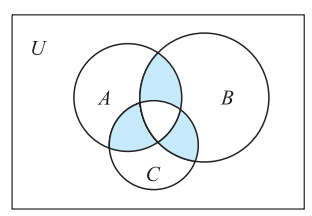
\includegraphics[width=6cm]{figures/C01-RV07.png}\end{center}}
\field{参考答案}{$(A\cap B\cap\complement_U C)\cup(A\cap C\cap\complement_U B)\cup(B\cap C\cap\complement_U A)$，即恰属于三个集合中两个的元素。}
{\small \field{关联知识}{S04 交集、并集及解集的联系（教材帮p.19、20 / PDF28、29）；S05 全集、补集与德摩根律（教材帮p.21 / PDF30）}
\field{方法与易错点}{先各自化简集合或解出约束，再在数轴上合并；有序数对交集通过联立方程求得。 易错：并集重复写元素；连接处一个闭端点也误删；把交集当并集。}
\field{答案依据}{答案册相关题组：PDF第8、9页（册内页7、8）；按当前题库原题逐项重算，不按旧版题号机械对套。}}

\itemhead{复习题一 · 第8题（教材p.29）}{XJ-B1-C01-RV-P029-Y1294}
\label{XJ-B1-C01-RV-P029-Y1294}
{\footnotesize 湘教版教材p.29 / PDF第36页 / 复习题一 / 第8题}
\field{原题}{判断下列命题的真假：
\subq{1}$a=b$ 是 $|a|=|b|$ 的必要条件；
\subq{2}$a>b$ 是 $a^2>b^2$ 的充分条件；
\subq{3}两个三角形的两组对应角分别相等是两个三角形相似的充要条件；
\subq{4}$(2x-1)x=0$ 是 $x=0$ 的充分而不必要条件。}
\field{参考答案}{依次为假、假、真、假。反例可分别取 $a=1,b=-1$；$a=-1,b=-2$；第（4）应为必要而不充分条件。}
{\small \field{关联知识}{L02 充分、必要、充要条件（教材帮p.30、31 / PDF39、40）}
\field{方法与易错点}{分别检查两个方向；用解集包含或具体反例判定，不凭句子位置猜方向。 易错：把“必要”箭头反写；只有一个方向证据便断言“不必要”；忽略给定论域。}
\field{答案依据}{答案册相关题组：PDF第8、9页（册内页7、8）；按当前题库原题逐项重算，不按旧版题号机械对套。}}

\itemhead{复习题一 · 第9题（教材p.29）}{XJ-B1-C01-RV-P029-Y1552}
\label{XJ-B1-C01-RV-P029-Y1552}
{\footnotesize 湘教版教材p.29 / PDF第36页 / 复习题一 / 第9题}
\field{原题}{下列命题中，哪些命题是“四边形是正方形”的充分条件？
\subq{1}对角线相等的菱形；
\subq{2}对角线互相垂直的矩形；
\subq{3}对角线相等的平行四边形；
\subq{4}有一个角是直角的菱形。}
\field{参考答案}{（1）（2）（4）。矩形且对角线垂直、菱形且对角线相等或有直角，均推出正方形。}
{\small \field{关联知识}{L02 充分、必要、充要条件（教材帮p.30、31 / PDF39、40）}
\field{方法与易错点}{分别检查两个方向；用解集包含或具体反例判定，不凭句子位置猜方向。 易错：把“必要”箭头反写；只有一个方向证据便断言“不必要”；忽略给定论域。}
\field{答案依据}{答案册相关题组：PDF第8、9页（册内页7、8）；按当前题库原题逐项重算，不按旧版题号机械对套。}}

\itemhead{复习题一 · 第10题（教材p.30）}{XJ-B1-C01-RV-P030-Y0307}
\label{XJ-B1-C01-RV-P030-Y0307}
{\footnotesize 湘教版教材p.30 / PDF第37页 / 复习题一 / 第10题}
\field{原题}{用全称量词或存在量词的符号表述命题：“任意三角形 $ABC$ 都有外接圆。”}
\field{参考答案}{$\forall\triangle ABC,\exists$ 圆 $O$，使 $A,B,C$ 都在圆 $O$ 上。存在的圆可随三角形而改变，不能交换两个量词次序。}
{\small \field{关联知识}{L03 全称、存在量词及真假的判定（教材帮p.38、39 / PDF47、48）}
\field{方法与易错点}{先确认量词、作用对象及论域，再采用任意性证明或实例反例。 易错：用几个满足的数证明全称命题；把“存在”理解为“唯一存在”。}
\field{答案依据}{答案册相关题组：PDF第8、9页（册内页7、8）；按当前题库原题逐项重算，不按旧版题号机械对套。}}

\itemhead{复习题一 · 第11题（教材p.30）}{XJ-B1-C01-RV-P030-Y0393}
\label{XJ-B1-C01-RV-P030-Y0393}
{\footnotesize 湘教版教材p.30 / PDF第37页 / 复习题一 / 第11题}
\field{原题}{写出下列命题的否定，并判断其真假：
\subq{1}$p$：$\exists a\in\mathbb R,\ a^2+1\ge0$；
\subq{2}$q$：所有偶数都是 2 的整数倍；
\subq{3}$r$：任意两个无理数的和都是无理数。}
\field{参考答案}{（1）$\forall a\in\mathbb R,a^2+1<0$，假；（2）存在偶数不是2的整数倍，假；（3）存在两个无理数的和不是无理数，真，如 $\sqrt2+(-\sqrt2)=0$。}
{\small \field{关联知识}{L04 含一个量词命题的否定（教材帮p.39、40 / PDF48、49）}
\field{方法与易错点}{分三步书写：保留论域、交换量词、否定断言，再判断新命题真假。 易错：只改量词不改结论；把不等号否定成反向但遗漏等号。}
\field{答案依据}{答案册相关题组：PDF第8、9页（册内页7、8）；按当前题库原题逐项重算，不按旧版题号机械对套。}}

\itemhead{复习题一 · 第12题（教材p.30）}{XJ-B1-C01-RV-P030-Y0711}
\label{XJ-B1-C01-RV-P030-Y0711}
{\footnotesize 湘教版教材p.30 / PDF第37页 / 复习题一 / 第12题}
\field{原题}{已知集合 $A=\{x\mid x+1>0\}$，$B=\{-2,-1,0,1\}$，求 $(\complement_{\mathbb R}A)\cap B$。}
\field{参考答案}{$\{-2,-1\}$。}
{\small \field{关联知识}{S05 全集、补集与德摩根律（教材帮p.21 / PDF30）；S04 交集、并集及解集的联系（教材帮p.19、20 / PDF28、29）}
\field{方法与易错点}{标出全集内的已知集合，取剩余区域，先算括号内部再补集。 易错：忘记全集范围；对“且”的否定仍写“且”；漏闭端点。}
\field{答案依据}{答案册相关题组：PDF第8、9页（册内页7、8）；按当前题库原题逐项重算，不按旧版题号机械对套。}}

\itemhead{复习题一 · 第13题（教材p.30）}{XJ-B1-C01-RV-P030-Y0753}
\label{XJ-B1-C01-RV-P030-Y0753}
{\footnotesize 湘教版教材p.30 / PDF第37页 / 复习题一 / 第13题}
\field{原题}{已知集合 $A,B$ 均为全集 $U=\{1,2,3,4\}$ 的子集，且 $\complement_U(A\cup B)=\{4\}$，$B=\{1,2\}$，求 $A\cap(\complement_U B)$。}
\field{参考答案}{$\{3\}$。由并集 $\{1,2,3\}$ 与 $B=\{1,2\}$，$A$ 必含3且不含4。}
{\small \field{关联知识}{S05 全集、补集与德摩根律（教材帮p.21 / PDF30）；S04 交集、并集及解集的联系（教材帮p.19、20 / PDF28、29）}
\field{方法与易错点}{标出全集内的已知集合，取剩余区域，先算括号内部再补集。 易错：忘记全集范围；对“且”的否定仍写“且”；漏闭端点。}
\field{答案依据}{答案册相关题组：PDF第8、9页（册内页7、8）；按当前题库原题逐项重算，不按旧版题号机械对套。}}

\itemhead{复习题一 · 第14题（教材p.30）}{XJ-B1-C01-RV-P030-Y0836}
\label{XJ-B1-C01-RV-P030-Y0836}
{\footnotesize 湘教版教材p.30 / PDF第37页 / 复习题一 / 第14题}
\field{原题}{在什么条件下，有 $[a,b]\cup[c,d]=[a,d]$？}
\field{参考答案}{在 $a\le b,c\le d$ 的区间约定下，充要条件为 $a\le c\le b\le d$。连接处 $c=b$ 可以取到；答案册原页也采用非严格不等式。}
{\small \field{关联知识}{S04 交集、并集及解集的联系（教材帮p.19、20 / PDF28、29）}
\field{方法与易错点}{先各自化简集合或解出约束，再在数轴上合并；有序数对交集通过联立方程求得。 易错：并集重复写元素；连接处一个闭端点也误删；把交集当并集。}
\field{答案依据}{答案册相关题组：PDF第8、9页（册内页7、8）；按当前题库原题逐项重算，不按旧版题号机械对套。}}

\itemhead{复习题一 · 第15题（教材p.30）}{XJ-B1-C01-RV-P030-Y0883}
\label{XJ-B1-C01-RV-P030-Y0883}
{\footnotesize 湘教版教材p.30 / PDF第37页 / 复习题一 / 第15题}
\field{原题}{为完成一项实地测量任务，夏令营的同学们成立了一支“测绘队”，需要 24 人参加测量，20 人参加计算，16 人参加绘图。测绘队的成员中很多同学是多面手，已知有 8 人只参加测量、计算，有 6 人只参加测量、绘图，有 4 人只参加计算、绘图，另有几人三项工作都参加了。试问这支测绘队至少有多少人？}
\field{参考答案}{至少30人。设三项都参加者为 $t$，则三类只参加一项的人数为 $10-t,8-t,6-t$，故 $0\le t\le6$；总人数为 $42-2t$，取 $t=6$ 得30。}
{\small \field{关联知识}{S06 Venn图、容斥与实际计数（教材帮p.22 / PDF31）}
\field{方法与易错点}{先画互不重叠区域，从最内层填写人数，再依据总人数或非负限制求解。 易错：把只参加两项的人数当作完整交集；重复计算三重交集；忽略一种都不参加。}
\field{答案依据}{答案册相关题组：PDF第8、9页（册内页7、8）；按当前题库原题逐项重算，不按旧版题号机械对套。}}

\itemhead{复习题一 · 第16题（教材p.30）}{XJ-B1-C01-RV-P030-Y1051}
\label{XJ-B1-C01-RV-P030-Y1051}
{\footnotesize 湘教版教材p.30 / PDF第37页 / 复习题一 / 第16题}
\field{原题}{已知 $p$：$1\le x\le2$，$q$：$a\le x\le a+2$。若 $\neg p$ 是 $\neg q$ 的必要而不充分条件，求 $a$ 的取值范围。}
\field{参考答案}{$a\in[0,1]$。$\neg q\Rightarrow\neg p$ 等价于 $p\Rightarrow q$，故 $[1,2]\subsetneq[a,a+2]$；由 $a\le1,a+2\ge2$ 得结果，两区间长度不同自动保证真包含。}
{\small \field{关联知识}{L02 充分、必要、充要条件（教材帮p.30、31 / PDF39、40）；S03 子集、真子集与集合相等（教材帮p.11、12、13 / PDF20、21、22）}
\field{方法与易错点}{分别检查两个方向；用解集包含或具体反例判定，不凭句子位置猜方向。 易错：把“必要”箭头反写；只有一个方向证据便断言“不必要”；忽略给定论域。}
\field{答案依据}{答案册相关题组：PDF第8、9页（册内页7、8）；按当前题库原题逐项重算，不按旧版题号机械对套。}}

\itemhead{复习题一 · 第17题（教材p.30）}{XJ-B1-C01-RV-P030-Y1286}
\label{XJ-B1-C01-RV-P030-Y1286}
{\footnotesize 湘教版教材p.30 / PDF第37页 / 复习题一 / 第17题}
\field{原题}{画出以方程 $(y-x)(y-x^2)=0$ 的解为坐标的所有点组成的图象。}
\field{参考答案}{图象为直线 $y=x$ 与抛物线 $y=x^2$ 的并，交点为 $(0,0),(1,1)$；并集图形本身不一定是一个函数的图象。}
\begin{center}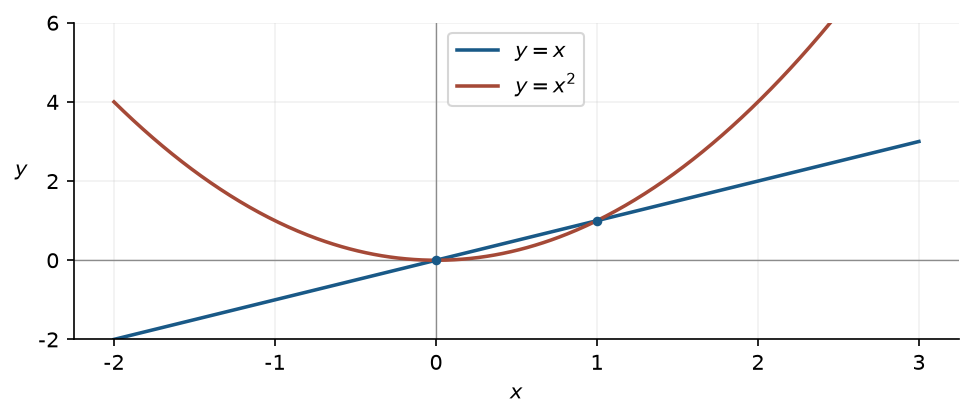
\includegraphics[width=.84\linewidth,height=.38\textheight,keepaspectratio]{figures/C01-RV030-17.png}\end{center}
{\small \field{关联知识}{S04 交集、并集及解集的联系（教材帮p.19、20 / PDF28、29）；F04 函数三种表示法、图象与读数（教材帮p.85、86、93、94 / PDF94、95、102、103）}
\field{方法与易错点}{先各自化简集合或解出约束，再在数轴上合并；有序数对交集通过联立方程求得。 易错：并集重复写元素；连接处一个闭端点也误删；把交集当并集。}
\field{答案依据}{答案册相关题组：PDF第8、9页（册内页7、8）；按当前题库原题逐项重算，不按旧版题号机械对套。}}

\itemhead{复习题一 · 第18题（教材p.30）}{XJ-B1-C01-RV-P030-Y1329}
\label{XJ-B1-C01-RV-P030-Y1329}
{\footnotesize 湘教版教材p.30 / PDF第37页 / 复习题一 / 第18题}
\field{原题}{已知集合 $A=\{1,3,a\}$，$B=\{1,a^2-a+1\}$，且 $A\cup B=A$，求 $a$ 的值。}
\field{参考答案}{$a=-1$ 或2。由 $B\subseteq A$，$a^2-a+1$ 必为1、3或 $a$；结合 $A$ 中元素互异排去 $a=0,1,3$ 等不合条件的候选。}
{\small \field{关联知识}{S01 集合、元素与常用数集（教材帮p.1、2 / PDF10、11）；S03 子集、真子集与集合相等（教材帮p.11、12、13 / PDF20、21、22）}
\field{方法与易错点}{先辨认研究对象和数集范围，再代入定义判断；含参集合逐个来源分类。 易错：把自然数集误作正整数集；混淆元素和单元素集合；候选参数造成元素重复。}
\field{答案依据}{答案册相关题组：PDF第8、9页（册内页7、8）；按当前题库原题逐项重算，不按旧版题号机械对套。}}

\itemhead{复习题一 · 第19题（教材p.30）}{XJ-B1-C01-RV-P030-Y1372}
\label{XJ-B1-C01-RV-P030-Y1372}
{\footnotesize 湘教版教材p.30 / PDF第37页 / 复习题一 / 第19题}
\field{原题}{设 $a,b,c$ 分别是 $\triangle ABC$ 的三条边，且 $a\le b\le c$。我们知道，$\angle C=90^\circ\Leftrightarrow a^2+b^2=c^2$。
\subq{1}证明：$\angle C<90^\circ\Leftrightarrow a^2+b^2>c^2$。
\subq{2}若 $\angle C>90^\circ$，请写出它的一个充要条件，并证明。}
\field{参考答案}{从 $A$ 向直线 $BC$ 作垂线，垂足为 $H$。因 $c\ge b$，锐角 $C$ 时 $H$ 在 $BC$ 内，记 $CH=d>0$，由勾股定理 $c^2=AH^2+(a-d)^2,b^2=AH^2+d^2$，得 $a^2+b^2-c^2=2ad>0$；直角 $C$ 时该差为0；钝角 $C$ 时 $H$ 在 $C$ 外侧，得差为 $-2ad<0$。三种情形互斥且完备，故两充要条件分别为 $a^2+b^2>c^2$ 和 $a^2+b^2<c^2$。}
{\small \field{关联知识}{L02 充分、必要、充要条件（教材帮p.30、31 / PDF39、40）}
\field{方法与易错点}{分别检查两个方向；用解集包含或具体反例判定，不凭句子位置猜方向。 易错：把“必要”箭头反写；只有一个方向证据便断言“不必要”；忽略给定论域。}
\field{答案依据}{答案册相关题组：PDF第8、9页（册内页7、8）；按当前题库原题逐项重算，不按旧版题号机械对套。}}

\section{第2章 一元二次函数、方程和不等式}
\itemhead{2.1 思考 · 未编号题组（教材p.32）}{XJ-B1-C02-TH-P032-Y0904}
\label{XJ-B1-C02-TH-P032-Y0904}
{\footnotesize 湘教版教材p.32 / PDF第39页 / 2.1 思考 / 未编号题组}
\field{原题}{观察章前图，你能从中找出一些不等关系并用数学语言描述吗？
\bankfig{C02-TH032}{0.78}}
\field{参考答案}{设车速为 $v$（km/h）。图中小客车道可写为 $90\le v\le120$；中间客货车道为 $80\le v\le100$；右侧客货车道为 $60\le v\le100$。例如同一道路可同时有最低和最高速度限制，不等式可描述允许的取值范围。}
{\small \field{关联知识}{I01 不等关系与作差比较（教材帮p.44 / PDF53）}
\field{方法与易错点}{作差、化简、定号、回写比较结论。 易错：看见负平方就写恒小于，遗漏平方为0的情形。}
\field{答案依据}{答案册未提供本栏目的独立对应答案；依据原题、教材概念补写参考回应。开放性总结不设唯一数值答案。}}

\itemhead{2.1 案例 · 案例1（教材p.33）}{XJ-B1-C02-CA-P033-Y0234}
\label{XJ-B1-C02-CA-P033-Y0234}
{\footnotesize 湘教版教材p.33 / PDF第40页 / 2.1 案例 / 案例1}
\field{原题}{2002 年在北京召开的第 24 届国际数学家大会的会标如图 2.1-2（1）所示，其中的几何图形取材于我国古代数学家对勾股定理的证明，如图 2.1-2（2）。图中的正方形 $ABCD$ 由 4 个全等的直角三角形和小正方形 $EFGH$ 组成。设直角三角形的两条直角边长分别为 $a,b\ (a\ne b)$，那么正方形 $ABCD$ 的边长为 $\sqrt{a^2+b^2}$。
\bankfig{C02-CA033}{0.62}
又 4 个直角三角形的面积之和为 $4\times\frac12ab=2ab$，正方形 $ABCD$ 的面积为 $a^2+b^2$，并且正方形 $ABCD$ 的面积大于 4 个直角三角形的面积之和，于是可得不等式 $a^2+b^2>2ab\ (a\ne b)$。}
\field{参考答案}{由面积分割，$a^2+b^2=2ab+(a-b)^2>2ab$，其中 $a\ne b$ 保证严格大于；若允许 $a=b$，应改为 $\ge$。}
{\small \field{关联知识}{I03 基本不等式、等号与最值建模（教材帮p.52、53、54 / PDF61、62、63）}
\field{方法与易错点}{列正数条件与固定量，构造基本不等式，解等号条件并代回实际限制。 易错：把一个下界误当最小值；多个等号条件不能同时实现；漏单位和整数限制。}
\field{答案依据}{答案册未提供本栏目的独立对应答案；依据原题、教材概念补写参考回应。开放性总结不设唯一数值答案。}}

\itemhead{2.1 案例 · 案例2（教材p.33）}{XJ-B1-C02-CA-P033-Y0951}
\label{XJ-B1-C02-CA-P033-Y0951}
{\footnotesize 湘教版教材p.33 / PDF第40页 / 2.1 案例 / 案例2}
\field{原题}{某商品以单价 10 元销售，每月可以卖出 2500 件。据市场调查，若单价每提高 1 元，月销售量就会减少 50 件。若提价后该商品的单价为 $x$ 元，则月销售量为 $[2500-50(x-10)]$ 件。于是不等关系“月销售收入不低于 30000 元”可以用不等式 $[2500-50(x-10)]x\ge30000$ 表示。}
\field{参考答案}{模型为 $50x(60-x)\ge30000$。若继续求解，得 $x\in[30-10\sqrt3,30+10\sqrt3]$，并满足提价与销量非负的实际范围 $10\le x\le60$。}
{\small \field{关联知识}{I06 恒成立、有解与范围内最值（教材帮p.71、72、73 / PDF80、81、82）；F03 函数求值、解析式与函数建模（教材帮p.80、87、88、89、90、131 / PDF89、96、97、98、99、140）}
\field{方法与易错点}{先明确主元及参数，分降次情况，再用判别式、配方或区间最值。 易错：严格号与非严格号混淆；把有解条件当恒成立；直接用全域判别式处理有限区间。}
\field{答案依据}{答案册未提供本栏目的独立对应答案；依据原题、教材概念补写参考回应。开放性总结不设唯一数值答案。}}

\itemhead{2.1 例题 · 例题1（教材p.34）}{XJ-B1-C02-EX-P034-Y0478}
\label{XJ-B1-C02-EX-P034-Y0478}
{\footnotesize 湘教版教材p.34 / PDF第41页 / 2.1 例题 / 例题1}
\field{原题}{比较 $(x+1)(x+3)$ 与 $(x+2)^2$ 的大小。}
\field{参考答案}{前者小于后者，因为 $(x+1)(x+3)-(x+2)^2=-1<0$。}
{\small \field{关联知识}{I01 不等关系与作差比较（教材帮p.44 / PDF53）}
\field{方法与易错点}{作差、化简、定号、回写比较结论。 易错：看见负平方就写恒小于，遗漏平方为0的情形。}
\field{答案依据}{例题原解位置：湘教版教材p.34及题库原图；独立编写可编辑参考解答。答案册此部分主要收练习、习题，不伪造例题答案册位置。}}

\itemhead{2.1 例题 · 例题2（教材p.34）}{XJ-B1-C02-EX-P034-Y0712}
\label{XJ-B1-C02-EX-P034-Y0712}
{\footnotesize 湘教版教材p.34 / PDF第41页 / 2.1 例题 / 例题2}
\field{原题}{$a\,\mathrm g$ 糖水中含有 $b\,\mathrm g$ 糖，若再添加 $m\,\mathrm g$ 糖（其中 $a>b>0,m>0$），生活常识告诉我们：添加的糖完全溶解后，糖水会更甜。根据这个生活常识，你能提炼出一个不等式吗？试给出证明。}
\field{参考答案}{$\dfrac{b+m}{a+m}>\dfrac ba$；两式之差为 $\dfrac{m(a-b)}{a(a+m)}>0$。}
{\small \field{关联知识}{I01 不等关系与作差比较（教材帮p.44 / PDF53）}
\field{方法与易错点}{作差、化简、定号、回写比较结论。 易错：看见负平方就写恒小于，遗漏平方为0的情形。}
\field{答案依据}{例题原解位置：湘教版教材p.34及题库原图；独立编写可编辑参考解答。答案册此部分主要收练习、习题，不伪造例题答案册位置。}}

\itemhead{p.34 练习 · 第1题（教材p.34）}{XJ-B1-C02-PR-P034-Y1377}
\label{XJ-B1-C02-PR-P034-Y1377}
{\footnotesize 湘教版教材p.34 / PDF第41页 / p.34 练习 / 第1题}
\field{原题}{比较大小：
\subq{1}$(x+1)(x-3)$ 与 $(x+2)(x-4)$；
\subq{2}$(x^2-1)^2$ 与 $x^4-x^2+1$；
\subq{3}$x^2+y^2+1$ 与 $2(x+y-1)$。}
\field{参考答案}{（1）前者大于后者，差为5；（2）前者不大于后者，差为 $-x^2$，$x=0$ 时相等；（3）前者大于后者，差为 $(x-1)^2+(y-1)^2+1>0$。}
{\small \field{关联知识}{I01 不等关系与作差比较（教材帮p.44 / PDF53）}
\field{方法与易错点}{作差、化简、定号、回写比较结论。 易错：看见负平方就写恒小于，遗漏平方为0的情形。}
\field{答案依据}{答案册相关题组：PDF第11页（册内页10）；按当前题库原题逐项重算，不按旧版题号机械对套。}}

\itemhead{p.34 练习 · 第2题（教材p.34）}{XJ-B1-C02-PR-P034-Y1563}
\label{XJ-B1-C02-PR-P034-Y1563}
{\footnotesize 湘教版教材p.34 / PDF第41页 / p.34 练习 / 第2题}
\field{原题}{若 $a<b<1$，试比较 $\dfrac a{a-1}$ 与 $\dfrac b{b-1}$ 的大小。}
\field{参考答案}{$\dfrac a{a-1}>\dfrac b{b-1}$，差为 $\dfrac{b-a}{(a-1)(b-1)}>0$。}
{\small \field{关联知识}{I01 不等关系与作差比较（教材帮p.44 / PDF53）}
\field{方法与易错点}{作差、化简、定号、回写比较结论。 易错：看见负平方就写恒小于，遗漏平方为0的情形。}
\field{答案依据}{答案册相关题组：PDF第11页（册内页10）；按当前题库原题逐项重算，不按旧版题号机械对套。}}

\itemhead{2.1 思考 · 未编号题组（教材p.35）}{XJ-B1-C02-TH-P035-Y0319}
\label{XJ-B1-C02-TH-P035-Y0319}
{\footnotesize 湘教版教材p.35 / PDF第42页 / 2.1 思考 / 未编号题组}
\field{原题}{类比等式，你能猜想出不等式的一些基本性质吗？}
\field{参考答案}{例如：$a>b\Rightarrow a+c>b+c$；乘正数方向不变，乘负数方向反向；$a>b,c>d\Rightarrow a+c>b+d$。同向不等式不能任意相减，乘除必须检查符号和非零条件。}
{\small \field{关联知识}{I02 不等式基本性质与符号条件（教材帮p.45、46 / PDF54、55）}
\field{方法与易错点}{每一步明确所乘除因子的正负与非零，或作差求证。 易错：未知符号就直接乘除；将 $c^2$ 当作必为正数而忘记 $c=0$。}
\field{答案依据}{答案册未提供本栏目的独立对应答案；依据原题、教材概念补写参考回应。开放性总结不设唯一数值答案。}}

\itemhead{2.1 例题 · 例题3（教材p.37）}{XJ-B1-C02-EX-P037-Y0431}
\label{XJ-B1-C02-EX-P037-Y0431}
{\footnotesize 湘教版教材p.37 / PDF第44页 / 2.1 例题 / 例题3}
\field{原题}{已知 $a>b,c<d$，求证：$a-c>b-d$。}
\field{参考答案}{由 $c<d$ 得 $-c>-d$，与 $a>b$ 同向相加即得 $a-c>b-d$。}
{\small \field{关联知识}{I02 不等式基本性质与符号条件（教材帮p.45、46 / PDF54、55）}
\field{方法与易错点}{每一步明确所乘除因子的正负与非零，或作差求证。 易错：未知符号就直接乘除；将 $c^2$ 当作必为正数而忘记 $c=0$。}
\field{答案依据}{例题原解位置：湘教版教材p.37及题库原图；独立编写可编辑参考解答。答案册此部分主要收练习、习题，不伪造例题答案册位置。}}

\itemhead{2.1 例题 · 例题4（教材p.37）}{XJ-B1-C02-EX-P037-Y0590}
\label{XJ-B1-C02-EX-P037-Y0590}
{\footnotesize 湘教版教材p.37 / PDF第44页 / 2.1 例题 / 例题4}
\field{原题}{求证：如果 $a>b>0$，且 $d>c>0$，那么 $\dfrac ac>\dfrac bd$。}
\field{参考答案}{$a/c>b/c>b/d$，两个步骤分别用 $c>0$、$d>c>0$。}
{\small \field{关联知识}{I02 不等式基本性质与符号条件（教材帮p.45、46 / PDF54、55）}
\field{方法与易错点}{每一步明确所乘除因子的正负与非零，或作差求证。 易错：未知符号就直接乘除；将 $c^2$ 当作必为正数而忘记 $c=0$。}
\field{答案依据}{例题原解位置：湘教版教材p.37及题库原图；独立编写可编辑参考解答。答案册此部分主要收练习、习题，不伪造例题答案册位置。}}

\itemhead{p.37 练习 · 第1题（教材p.37）}{XJ-B1-C02-PR-P037-Y0875}
\label{XJ-B1-C02-PR-P037-Y0875}
{\footnotesize 湘教版教材p.37 / PDF第44页 / p.37 练习 / 第1题}
\field{原题}{判断下列命题的真假，并说明理由：
\subq{1}若 $a>b$，则 $ca>cb$；
\subq{2}若 $a>b$，则 $ac^2>bc^2$；
\subq{3}若 $a>b,c\ne0$，则 $\dfrac ac>\dfrac bc$；
\subq{4}若 $a>b,c\ne0$，则 $\dfrac a{c^2}>\dfrac b{c^2}$。}
\field{参考答案}{依次为假、假、假、真。前三项分别取 $c=-1,c=0,c=-1$ 即可构造反例；第四项除数 $c^2>0$。}
{\small \field{关联知识}{I02 不等式基本性质与符号条件（教材帮p.45、46 / PDF54、55）}
\field{方法与易错点}{每一步明确所乘除因子的正负与非零，或作差求证。 易错：未知符号就直接乘除；将 $c^2$ 当作必为正数而忘记 $c=0$。}
\field{答案依据}{答案册相关题组：PDF第11页（册内页10）；按当前题库原题逐项重算，不按旧版题号机械对套。}}

\itemhead{p.37 练习 · 第2题（教材p.37）}{XJ-B1-C02-PR-P037-Y1148}
\label{XJ-B1-C02-PR-P037-Y1148}
{\footnotesize 湘教版教材p.37 / PDF第44页 / p.37 练习 / 第2题}
\field{原题}{回答下列问题：
\subq{1}若 $a>b$，且 $c>d$，能否判断 $a-c$ 与 $b-d$ 的大小？举例说明。
\subq{2}若 $a>b$，且 $c<d$，能否判断 $a+c$ 与 $b+d$ 的大小？举例说明。
\subq{3}若 $a>b$，且 $c>d$，能否判断 $ac$ 与 $bd$ 的大小？举例说明。
\subq{4}若 $a>b,c<d$，且 $c\ne0,d\ne0$，能否判断 $\dfrac ac$ 与 $\dfrac bd$ 的大小？举例说明。}
\field{参考答案}{四问均不能。各给出两组 $(a,b,c,d)$：（1）$(3,1,2,1)$、$(2,1,4,1)$；（2）$(3,1,0,1)$、$(2,1,0,3)$；（3）$(2,1,2,1)$、$(-1,-2,-1,-2)$；（4）$(2,1,1,2)$、$(3,1,-2,-1)$。每组均满足该小问题设，所得比较方向相反。}
{\small \field{关联知识}{I02 不等式基本性质与符号条件（教材帮p.45、46 / PDF54、55）}
\field{方法与易错点}{每一步明确所乘除因子的正负与非零，或作差求证。 易错：未知符号就直接乘除；将 $c^2$ 当作必为正数而忘记 $c=0$。}
\field{答案依据}{答案册相关题组：PDF第11页（册内页10）；按当前题库原题逐项重算，不按旧版题号机械对套。}}

\itemhead{p.37 练习 · 第3题（教材p.37）}{XJ-B1-C02-PR-P037-Y1391}
\label{XJ-B1-C02-PR-P037-Y1391}
{\footnotesize 湘教版教材p.37 / PDF第44页 / p.37 练习 / 第3题}
\field{原题}{求证：
\subq{1}若 $a>b>0$，且 $c<d<0$，则 $ac<bd$；
\subq{2}若 $a>b$，且 $a,b$ 同号，$c>0$，则 $\dfrac ca<\dfrac cb$；
\subq{3}若 $a>b>0$，且 $c>d>0$，则 $\sqrt{\dfrac ad}>\sqrt{\dfrac bc}$。}
\field{参考答案}{（1）$ac<bc<bd$；（2）$\dfrac ca-\dfrac cb=\dfrac{c(b-a)}{ab}<0$；（3）$a/d>b/d>b/c>0$，再利用平方根保序。}
{\small \field{关联知识}{I02 不等式基本性质与符号条件（教材帮p.45、46 / PDF54、55）}
\field{方法与易错点}{每一步明确所乘除因子的正负与非零，或作差求证。 易错：未知符号就直接乘除；将 $c^2$ 当作必为正数而忘记 $c=0$。}
\field{答案依据}{答案册相关题组：PDF第11页（册内页10）；按当前题库原题逐项重算，不按旧版题号机械对套。}}

\itemhead{2.1 例题 · 例题5（教材p.39）}{XJ-B1-C02-EX-P039-Y0303}
\label{XJ-B1-C02-EX-P039-Y0303}
{\footnotesize 湘教版教材p.39 / PDF第46页 / 2.1 例题 / 例题5}
\field{原题}{设 $a,b$ 为正数，证明下列不等式：
\subq{1}$a+\dfrac1a\ge2$；
\subq{2}$\dfrac ba+\dfrac ab\ge2$。}
\field{参考答案}{（1）$a+1/a-2=(a-1)^2/a\ge0$，等号当 $a=1$；（2）$b/a+a/b-2=(a-b)^2/(ab)\ge0$，等号当 $a=b$。}
{\small \field{关联知识}{I03 基本不等式、等号与最值建模（教材帮p.52、53、54 / PDF61、62、63）}
\field{方法与易错点}{列正数条件与固定量，构造基本不等式，解等号条件并代回实际限制。 易错：把一个下界误当最小值；多个等号条件不能同时实现；漏单位和整数限制。}
\field{答案依据}{例题原解位置：湘教版教材p.39及题库原图；独立编写可编辑参考解答。答案册此部分主要收练习、习题，不伪造例题答案册位置。}}

\itemhead{2.1 例题 · 例题6（教材p.39）}{XJ-B1-C02-EX-P039-Y0870}
\label{XJ-B1-C02-EX-P039-Y0870}
{\footnotesize 湘教版教材p.39 / PDF第46页 / 2.1 例题 / 例题6}
\field{原题}{对任意三个正实数 $a,b,c$，求证：$a+b+c\ge\sqrt{ab}+\sqrt{bc}+\sqrt{ca}$，当且仅当 $a=b=c$ 时等号成立。}
\field{参考答案}{分别写 $a+b\ge2\sqrt{ab}$、$b+c\ge2\sqrt{bc}$、$c+a\ge2\sqrt{ca}$，相加除以2即可；等号当且仅当 $a=b=c$。}
{\small \field{关联知识}{I03 基本不等式、等号与最值建模（教材帮p.52、53、54 / PDF61、62、63）}
\field{方法与易错点}{列正数条件与固定量，构造基本不等式，解等号条件并代回实际限制。 易错：把一个下界误当最小值；多个等号条件不能同时实现；漏单位和整数限制。}
\field{答案依据}{例题原解位置：湘教版教材p.39及题库原图；独立编写可编辑参考解答。答案册此部分主要收练习、习题，不伪造例题答案册位置。}}

\itemhead{2.1 例题 · 例题7（教材p.39）}{XJ-B1-C02-EX-P039-Y1344}
\label{XJ-B1-C02-EX-P039-Y1344}
{\footnotesize 湘教版教材p.39 / PDF第46页 / 2.1 例题 / 例题7}
\field{原题}{已知 $0<x<1$，求 $\sqrt{x(1-x)}$ 的最大值。}
\field{参考答案}{最大值 $1/2$，在 $x=1/2$ 取得，因为 $x(1-x)\le[(x+1-x)/2]^2=1/4$。}
{\small \field{关联知识}{I03 基本不等式、等号与最值建模（教材帮p.52、53、54 / PDF61、62、63）}
\field{方法与易错点}{列正数条件与固定量，构造基本不等式，解等号条件并代回实际限制。 易错：把一个下界误当最小值；多个等号条件不能同时实现；漏单位和整数限制。}
\field{答案依据}{例题原解位置：湘教版教材p.39及题库原图；独立编写可编辑参考解答。答案册此部分主要收练习、习题，不伪造例题答案册位置。}}

\itemhead{p.40 练习 · 第1题（教材p.40）}{XJ-B1-C02-PR-P040-Y0217}
\label{XJ-B1-C02-PR-P040-Y0217}
{\footnotesize 湘教版教材p.40 / PDF第47页 / p.40 练习 / 第1题}
\field{原题}{计算下列两个数的算术平均数与几何平均数。
\subq{1}4，16；
\subq{2}3，12；
\subq{3}1，$4a^2\ (a>0)$；
\subq{4}$5a$，$5a\ (a>0)$。}
\field{参考答案}{各题的“算术平均数，几何平均数”依次为 $(10,8)$，$(15/2,6)$，$((1+4a^2)/2,2a)$，$(5a,5a)$。}
{\small \field{关联知识}{I03 基本不等式、等号与最值建模（教材帮p.52、53、54 / PDF61、62、63）}
\field{方法与易错点}{列正数条件与固定量，构造基本不等式，解等号条件并代回实际限制。 易错：把一个下界误当最小值；多个等号条件不能同时实现；漏单位和整数限制。}
\field{答案依据}{答案册相关题组：PDF第11页（册内页10）；按当前题库原题逐项重算，不按旧版题号机械对套。}}

\itemhead{p.40 练习 · 第2题（教材p.40）}{XJ-B1-C02-PR-P040-Y0349}
\label{XJ-B1-C02-PR-P040-Y0349}
{\footnotesize 湘教版教材p.40 / PDF第47页 / p.40 练习 / 第2题}
\field{原题}{已知 $a,b,c\in\mathbb R$，求证：$a^2+b^2+c^2\ge ab+bc+ac$。}
\field{参考答案}{左减右等于 $\tfrac12[(a-b)^2+(b-c)^2+(c-a)^2]\ge0$；等号当且仅当 $a=b=c$。}
{\small \field{关联知识}{I03 基本不等式、等号与最值建模（教材帮p.52、53、54 / PDF61、62、63）}
\field{方法与易错点}{列正数条件与固定量，构造基本不等式，解等号条件并代回实际限制。 易错：把一个下界误当最小值；多个等号条件不能同时实现；漏单位和整数限制。}
\field{答案依据}{答案册相关题组：PDF第11页（册内页10）；按当前题库原题逐项重算，不按旧版题号机械对套。}}

\itemhead{p.40 练习 · 第3题（教材p.40）}{XJ-B1-C02-PR-P040-Y0406}
\label{XJ-B1-C02-PR-P040-Y0406}
{\footnotesize 湘教版教材p.40 / PDF第47页 / p.40 练习 / 第3题}
\field{原题}{已知 $x>1$，求 $x+\dfrac4{x-1}$ 的最小值。}
\field{参考答案}{$x+4/(x-1)=(x-1)+4/(x-1)+1\ge5$，在 $x=3$ 取得最小值5。}
{\small \field{关联知识}{I03 基本不等式、等号与最值建模（教材帮p.52、53、54 / PDF61、62、63）}
\field{方法与易错点}{列正数条件与固定量，构造基本不等式，解等号条件并代回实际限制。 易错：把一个下界误当最小值；多个等号条件不能同时实现；漏单位和整数限制。}
\field{答案依据}{答案册相关题组：PDF第11页（册内页10）；按当前题库原题逐项重算，不按旧版题号机械对套。}}

\itemhead{p.40 练习 · 第4题（教材p.40）}{XJ-B1-C02-PR-P040-Y0461}
\label{XJ-B1-C02-PR-P040-Y0461}
{\footnotesize 湘教版教材p.40 / PDF第47页 / p.40 练习 / 第4题}
\field{原题}{已知 $0\le x\le1$，求 $(1+x)\cdot x^2\cdot(1-x)$ 的最大值。}
\field{参考答案}{原式 $=x^2(1-x^2)\le1/4$，在 $x=\sqrt2/2$ 取得最大值 $1/4$。}
{\small \field{关联知识}{I03 基本不等式、等号与最值建模（教材帮p.52、53、54 / PDF61、62、63）}
\field{方法与易错点}{列正数条件与固定量，构造基本不等式，解等号条件并代回实际限制。 易错：把一个下界误当最小值；多个等号条件不能同时实现；漏单位和整数限制。}
\field{答案依据}{答案册相关题组：PDF第11页（册内页10）；按当前题库原题逐项重算，不按旧版题号机械对套。}}

\itemhead{2.1 思考 · 未编号题组（教材p.40）}{XJ-B1-C02-TH-P040-Y0846}
\label{XJ-B1-C02-TH-P040-Y0846}
{\footnotesize 湘教版教材p.40 / PDF第47页 / 2.1 思考 / 未编号题组}
\field{原题}{\subq{1}把 12 写成两个正数的乘积，当这两个正数取什么值时，它们的和最小？
\subq{2}把 25 写成两个正数的和，当这两个正数取什么值时，它们的积最大？
\subq{3}由（1）（2）你能概括出什么结论？}
\field{参考答案}{（1）两个数均为 $2\sqrt3$ 时和最小为 $4\sqrt3$；（2）两个数均为 $25/2$ 时积最大为 $625/4$；（3）正数定积时和有最小值，定和时积有最大值，均在两数相等时取得。}
{\small \field{关联知识}{I03 基本不等式、等号与最值建模（教材帮p.52、53、54 / PDF61、62、63）}
\field{方法与易错点}{列正数条件与固定量，构造基本不等式，解等号条件并代回实际限制。 易错：把一个下界误当最小值；多个等号条件不能同时实现；漏单位和整数限制。}
\field{答案依据}{答案册未提供本栏目的独立对应答案；依据原题、教材概念补写参考回应。开放性总结不设唯一数值答案。}}

\itemhead{2.1 例题 · 例题8（教材p.41）}{XJ-B1-C02-EX-P041-Y0698}
\label{XJ-B1-C02-EX-P041-Y0698}
{\footnotesize 湘教版教材p.41 / PDF第48页 / 2.1 例题 / 例题8}
\field{原题}{某单位欲建造一间底面为矩形且面积为 $12\,\mathrm{m^2}$ 的背面靠墙的小屋。房屋正面的造价为 $1200$ 元/$\mathrm{m^2}$，侧面的造价为 $800$ 元/$\mathrm{m^2}$，屋顶的造价为 5200 元。如果墙高为 $3\,\mathrm m$，且不计房屋背面和底面的费用，问怎样设计房屋能使总造价最低？最低总造价是多少元？}
\field{参考答案}{设正面宽 $x$、进深 $y$，$xy=12$，造价 $C=3600x+4800y+5200\ge34000$。等号需 $3600x=4800y$，解得 $x=4,y=3$（米），最低造价34000元。}
{\small \field{关联知识}{I03 基本不等式、等号与最值建模（教材帮p.52、53、54 / PDF61、62、63）；F03 函数求值、解析式与函数建模（教材帮p.80、87、88、89、90、131 / PDF89、96、97、98、99、140）}
\field{方法与易错点}{列正数条件与固定量，构造基本不等式，解等号条件并代回实际限制。 易错：把一个下界误当最小值；多个等号条件不能同时实现；漏单位和整数限制。}
\field{答案依据}{例题原解位置：湘教版教材p.41及题库原图；独立编写可编辑参考解答。答案册此部分主要收练习、习题，不伪造例题答案册位置。}}

\itemhead{2.1 例题 · 例题9（教材p.41）}{XJ-B1-C02-EX-P041-Y1378}
\label{XJ-B1-C02-EX-P041-Y1378}
{\footnotesize 湘教版教材p.41 / PDF第48页 / 2.1 例题 / 例题9}
\field{原题}{某公司设计了如图 2.1-5 所示的一块绿化景观地带，两条平行线段的两端用半圆弧相连接。已知这块绿化景观地带的内圈周长为 $400\,\mathrm m$，当平行线段的长设计为多少时，中间矩形区域的面积最大？
\bankfig{C02-EX041}{0.46}}
\field{参考答案}{设平行线段长为 $l$、两线间距为 $w$，则 $2l+\pi w=400$。$lw=l(400-2l)/\pi$ 在 $l=100$ 米时最大，为 $20000/\pi$ 平方米。}
{\small \field{关联知识}{I03 基本不等式、等号与最值建模（教材帮p.52、53、54 / PDF61、62、63）；F03 函数求值、解析式与函数建模（教材帮p.80、87、88、89、90、131 / PDF89、96、97、98、99、140）}
\field{方法与易错点}{列正数条件与固定量，构造基本不等式，解等号条件并代回实际限制。 易错：把一个下界误当最小值；多个等号条件不能同时实现；漏单位和整数限制。}
\field{答案依据}{例题原解位置：湘教版教材p.41及题库原图；独立编写可编辑参考解答。答案册此部分主要收练习、习题，不伪造例题答案册位置。}}

\itemhead{p.42 练习 · 第1题（教材p.42）}{XJ-B1-C02-PR-P042-Y0646}
\label{XJ-B1-C02-PR-P042-Y0646}
{\footnotesize 湘教版教材p.42 / PDF第49页 / p.42 练习 / 第1题}
\field{原题}{甲、乙两同学分别解“设 $x\in[1,+\infty)$，求二次函数 $y=2x^2+1$ 的最小值”的过程如下：
\par 甲：$y=2x^2+1\ge2\sqrt{2x^2\cdot1}=2\sqrt2x$，又 $x\ge1$，所以 $2\sqrt2x\ge2\sqrt2$。从而 $y\ge2\sqrt2x\ge2\sqrt2$，即 $y$ 的最小值是 $2\sqrt2$。
\par 乙：因为函数 $y=2x^2+1$ 在区间 $[1,+\infty)$ 上的图象随着 $x$ 增大而逐渐上升，即 $y$ 随 $x$ 增大而增大，所以 $y$ 的最小值是 $2\times1^2+1=3$。
\par 试判断谁错，错在何处？}
\field{参考答案}{甲错。两次不等式取等号分别要求 $x=1/\sqrt2$ 和 $x=1$，不能同时成立；$2\sqrt2$ 只是一个未必可取的下界。乙正确，最小值为3。}
{\small \field{关联知识}{I03 基本不等式、等号与最值建模（教材帮p.52、53、54 / PDF61、62、63）}
\field{方法与易错点}{列正数条件与固定量，构造基本不等式，解等号条件并代回实际限制。 易错：把一个下界误当最小值；多个等号条件不能同时实现；漏单位和整数限制。}
\field{答案依据}{答案册相关题组：PDF第11页（册内页10）；按当前题库原题逐项重算，不按旧版题号机械对套。}}

\itemhead{p.42 练习 · 第2题（教材p.42）}{XJ-B1-C02-PR-P042-Y1011}
\label{XJ-B1-C02-PR-P042-Y1011}
{\footnotesize 湘教版教材p.42 / PDF第49页 / p.42 练习 / 第2题}
\field{原题}{如图，动物园要以墙体为背面，用钢筋网围成四间面积相同的矩形虎笼。
\bankfig{C02-PR042}{0.58}
\subq{1}现有可围 $36\,\mathrm m$ 长钢筋网的材料，每间虎笼的长、宽各设计为多少时，可使每间虎笼的面积最大？
\subq{2}若每间虎笼的面积为 $20\,\mathrm{m^2}$，则每间虎笼的长、宽各设计为多少时，可使围成四间虎笼的钢筋网总长最小？}
\field{参考答案}{设每间沿墙方向宽 $w$、垂直墙长 $l$，钢筋网长 $4w+5l$。（1）$4w+5l=36$ 时 $l=3.6,w=4.5$ 米，每间最大面积16.2平方米；（2）$lw=20$ 时 $l=4,w=5$ 米，总长最小40米。两小问与答案册放大原页一致；方向名称按图中沿墙、垂直墙明确，避免混淆长宽。}
{\small \field{关联知识}{I03 基本不等式、等号与最值建模（教材帮p.52、53、54 / PDF61、62、63）；F03 函数求值、解析式与函数建模（教材帮p.80、87、88、89、90、131 / PDF89、96、97、98、99、140）}
\field{方法与易错点}{列正数条件与固定量，构造基本不等式，解等号条件并代回实际限制。 易错：把一个下界误当最小值；多个等号条件不能同时实现；漏单位和整数限制。}
\field{答案依据}{答案册相关题组：PDF第11页（册内页10）；按当前题库原题逐项重算，不按旧版题号机械对套。}}

\itemhead{p.42 练习 · 第3题（教材p.42）}{XJ-B1-C02-PR-P042-Y1470}
\label{XJ-B1-C02-PR-P042-Y1470}
{\footnotesize 湘教版教材p.42 / PDF第49页 / p.42 练习 / 第3题}
\field{原题}{现在要求设计一张单栏的竖向张贴的海报，它的中间印刷面积为 $128\,\mathrm{dm^2}$，上下空白各 $2\,\mathrm{dm}$，左右空白各 $1\,\mathrm{dm}$，如何确定海报尺寸使四周空白面积最小？}
\field{参考答案}{设印刷区宽 $x$、高 $y$，$xy=128$，空白面积为 $4x+2y+8\ge72$。等号当 $x=8,y=16$；海报总宽10 dm、高20 dm，最小空白面积72平方分米。}
{\small \field{关联知识}{I03 基本不等式、等号与最值建模（教材帮p.52、53、54 / PDF61、62、63）；F03 函数求值、解析式与函数建模（教材帮p.80、87、88、89、90、131 / PDF89、96、97、98、99、140）}
\field{方法与易错点}{列正数条件与固定量，构造基本不等式，解等号条件并代回实际限制。 易错：把一个下界误当最小值；多个等号条件不能同时实现；漏单位和整数限制。}
\field{答案依据}{答案册相关题组：PDF第11页（册内页10）；按当前题库原题逐项重算，不按旧版题号机械对套。}}

\itemhead{习题2.1 · 第1题（教材p.43）}{XJ-B1-C02-HW-P043-Y0450}
\label{XJ-B1-C02-HW-P043-Y0450}
{\footnotesize 湘教版教材p.43 / PDF第50页 / 习题2.1 / 第1题}
\field{原题}{比较 $(2a+1)(a-3)$ 与 $(a-6)(2a+7)+45$ 的大小。}
\field{参考答案}{前者小于后者，作差为 $-6<0$；两式分别展开为 $2a^2-5a-3$ 与 $2a^2-5a+3$。}
{\small \field{关联知识}{I01 不等关系与作差比较（教材帮p.44 / PDF53）}
\field{方法与易错点}{作差、化简、定号、回写比较结论。 易错：看见负平方就写恒小于，遗漏平方为0的情形。}
\field{答案依据}{答案册相关题组：PDF第12、13页（册内页11、12）；按当前题库原题逐项重算，不按旧版题号机械对套。}}

\itemhead{习题2.1 · 第2题（教材p.43）}{XJ-B1-C02-HW-P043-Y0493}
\label{XJ-B1-C02-HW-P043-Y0493}
{\footnotesize 湘教版教材p.43 / PDF第50页 / 习题2.1 / 第2题}
\field{原题}{比较下列各题中两个代数式的大小：
\subq{1}$(\sqrt m-1)^2$ 与 $(\sqrt m+1)^2$；
\subq{2}$(x^2+\sqrt2x+1)(x^2-\sqrt2x+1)$ 与 $(x^2+x+1)(x^2-x+1)$。}
\field{参考答案}{（1）差为 $-4\sqrt m\le0$，$m=0$ 时相等，$m>0$ 时前者小；（2）差为 $-x^2\le0$，$x=0$ 时相等，其余前者小。不可把非严格不等式写成恒严格小于。}
{\small \field{关联知识}{I01 不等关系与作差比较（教材帮p.44 / PDF53）}
\field{方法与易错点}{作差、化简、定号、回写比较结论。 易错：看见负平方就写恒小于，遗漏平方为0的情形。}
\field{答案依据}{答案册相关题组：PDF第12、13页（册内页11、12）；按当前题库原题逐项重算，不按旧版题号机械对套。}}

\itemhead{习题2.1 · 第3题（教材p.43）}{XJ-B1-C02-HW-P043-Y0634}
\label{XJ-B1-C02-HW-P043-Y0634}
{\footnotesize 湘教版教材p.43 / PDF第50页 / 习题2.1 / 第3题}
\field{原题}{如果 $a<b<0$，则有（用“$>$”或“$<$”填空）：
\subq{1}$-a\blank-b$；
\subq{2}$\dfrac1a\blank\dfrac1b$；
\subq{3}$\sqrt{a^2}\blank\sqrt{b^2}$；
\subq{4}$\dfrac ba\blank1$。}
\field{参考答案}{依次为 $>,>,>,<$。}
{\small \field{关联知识}{I02 不等式基本性质与符号条件（教材帮p.45、46 / PDF54、55）}
\field{方法与易错点}{每一步明确所乘除因子的正负与非零，或作差求证。 易错：未知符号就直接乘除；将 $c^2$ 当作必为正数而忘记 $c=0$。}
\field{答案依据}{答案册相关题组：PDF第12、13页（册内页11、12）；按当前题库原题逐项重算，不按旧版题号机械对套。}}

\itemhead{习题2.1 · 第4题（教材p.43）}{XJ-B1-C02-HW-P043-Y0819}
\label{XJ-B1-C02-HW-P043-Y0819}
{\footnotesize 湘教版教材p.43 / PDF第50页 / 习题2.1 / 第4题}
\field{原题}{下列结论是否成立？若成立，试说明理由；若不成立，试举出反例。
\subq{1}如果 $c-a>c-b$，那么 $a<b$；
\subq{2}若 $ab>c,b>0$，则 $a>\dfrac cb$；
\subq{3}若 $ac>bc$，则 $a>b$；
\subq{4}若 $a>b,c>d$，则 $a-c>b-d$。}
\field{参考答案}{（1）（2）成立；（3）不成立，取 $a=1,b=2,c=-1$；（4）不成立，取 $a=2,b=1,c=4,d=1$。}
{\small \field{关联知识}{I02 不等式基本性质与符号条件（教材帮p.45、46 / PDF54、55）}
\field{方法与易错点}{每一步明确所乘除因子的正负与非零，或作差求证。 易错：未知符号就直接乘除；将 $c^2$ 当作必为正数而忘记 $c=0$。}
\field{答案依据}{答案册相关题组：PDF第12、13页（册内页11、12）；按当前题库原题逐项重算，不按旧版题号机械对套。}}

\itemhead{习题2.1 · 第5题（教材p.43）}{XJ-B1-C02-HW-P043-Y1062}
\label{XJ-B1-C02-HW-P043-Y1062}
{\footnotesize 湘教版教材p.43 / PDF第50页 / 习题2.1 / 第5题}
\field{原题}{证明下列不等式，并讨论等号成立的条件：
\subq{1}若 $a>0$，则 $a+a^3\ge2a^2$；
\subq{2}若 $ab=4$，则 $a^2+b^2\ge8$；
\subq{3}若 $-1\le x\le1$，则 $\sqrt{x^2(1-x^2)}\le\dfrac12$；
\subq{4}若 $ab\ne0$，则 $\left|\dfrac ba+\dfrac ab\right|\ge2$；
\subq{5}对任意实数 $a$ 和 $b$，$a^2+b^2+\dfrac4{a^2+b^2+1}\ge3$。}
\field{参考答案}{（1）差为 $a(a-1)^2\ge0$，等号 $a=1$；（2）差为 $(a-b)^2\ge0$，等号 $a=b=2$ 或 $a=b=-2$；（3）$x^2(1-x^2)\le1/4$，等号 $x=\pm1/\sqrt2$；（4）令 $t=|a/b|>0$，$t+1/t\ge2$，等号 $|a|=|b|$；（5）置 $t=a^2+b^2+1\ge1$，原式 $=t+4/t-1\ge3$，等号 $a^2+b^2=1$。}
{\small \field{关联知识}{I03 基本不等式、等号与最值建模（教材帮p.52、53、54 / PDF61、62、63）}
\field{方法与易错点}{列正数条件与固定量，构造基本不等式，解等号条件并代回实际限制。 易错：把一个下界误当最小值；多个等号条件不能同时实现；漏单位和整数限制。}
\field{答案依据}{答案册相关题组：PDF第12、13页（册内页11、12）；按当前题库原题逐项重算，不按旧版题号机械对套。}}

\itemhead{习题2.1 · 第6题（教材p.43）}{XJ-B1-C02-HW-P043-Y1406}
\label{XJ-B1-C02-HW-P043-Y1406}
{\footnotesize 湘教版教材p.43 / PDF第50页 / 习题2.1 / 第6题}
\field{原题}{\subq{1}把 36 写成两个正数的乘积，当这两个正数取什么值时，它们的和最小？
\subq{2}把 18 写成两个正数的和，当这两个正数取什么值时，它们的积最大？}
\field{参考答案}{（1）均为6时，和最小12；（2）均为9时，积最大81。}
{\small \field{关联知识}{I03 基本不等式、等号与最值建模（教材帮p.52、53、54 / PDF61、62、63）}
\field{方法与易错点}{列正数条件与固定量，构造基本不等式，解等号条件并代回实际限制。 易错：把一个下界误当最小值；多个等号条件不能同时实现；漏单位和整数限制。}
\field{答案依据}{答案册相关题组：PDF第12、13页（册内页11、12）；按当前题库原题逐项重算，不按旧版题号机械对套。}}

\itemhead{习题2.1 · 第7题（教材p.43）}{XJ-B1-C02-HW-P043-Y1506}
\label{XJ-B1-C02-HW-P043-Y1506}
{\footnotesize 湘教版教材p.43 / PDF第50页 / 习题2.1 / 第7题}
\field{原题}{\subq{1}已知 $x>1$，求 $x+\dfrac1{x-1}$ 的最小值；
\subq{2}已知 $0<x<10$，求 $\sqrt{x(10-x)}$ 的最大值。}
\field{参考答案}{（1）最小值3，$x=2$ 时取得；（2）最大值5，$x=5$ 时取得。}
{\small \field{关联知识}{I03 基本不等式、等号与最值建模（教材帮p.52、53、54 / PDF61、62、63）}
\field{方法与易错点}{列正数条件与固定量，构造基本不等式，解等号条件并代回实际限制。 易错：把一个下界误当最小值；多个等号条件不能同时实现；漏单位和整数限制。}
\field{答案依据}{答案册相关题组：PDF第12、13页（册内页11、12）；按当前题库原题逐项重算，不按旧版题号机械对套。}}

\itemhead{习题2.1 · 第8题（教材p.44）}{XJ-B1-C02-HW-P044-Y0220}
\label{XJ-B1-C02-HW-P044-Y0220}
{\footnotesize 湘教版教材p.44 / PDF第51页 / 习题2.1 / 第8题}
\field{原题}{如图，在一块锐角三角形空地中欲建一个面积最大的内接矩形花园（阴影部分）。则花园的长、宽分别为多少时面积最大？最大面积是多少？
\bankfig{C02-HW044}{0.43}}
\field{参考答案}{由图中底边及高均为40米，相似关系得矩形两边 $x+y=40$；两边均为20米时面积最大400平方米。}
{\small \field{关联知识}{I03 基本不等式、等号与最值建模（教材帮p.52、53、54 / PDF61、62、63）；F03 函数求值、解析式与函数建模（教材帮p.80、87、88、89、90、131 / PDF89、96、97、98、99、140）}
\field{方法与易错点}{列正数条件与固定量，构造基本不等式，解等号条件并代回实际限制。 易错：把一个下界误当最小值；多个等号条件不能同时实现；漏单位和整数限制。}
\field{答案依据}{答案册相关题组：PDF第12、13页（册内页11、12）；按当前题库原题逐项重算，不按旧版题号机械对套。}}

\itemhead{习题2.1 · 第9题（教材p.44）}{XJ-B1-C02-HW-P044-Y0732}
\label{XJ-B1-C02-HW-P044-Y0732}
{\footnotesize 湘教版教材p.44 / PDF第51页 / 习题2.1 / 第9题}
\field{原题}{利用不等式的性质证明下列不等式：
\subq{1}若 $a<b,c<0$，则 $(a-b)c>0$；
\subq{2}若 $a<0,-1<b<0$，则 $a<ab^2<ab$。}
\field{参考答案}{（1）$a-b<0,c<0$，故积大于0；（2）$0<b^2<1$，乘 $a<0$ 得 $a<ab^2<0$，又 $ab>0$，故 $a<ab^2<ab$。}
{\small \field{关联知识}{I02 不等式基本性质与符号条件（教材帮p.45、46 / PDF54、55）}
\field{方法与易错点}{每一步明确所乘除因子的正负与非零，或作差求证。 易错：未知符号就直接乘除；将 $c^2$ 当作必为正数而忘记 $c=0$。}
\field{答案依据}{答案册相关题组：PDF第12、13页（册内页11、12）；按当前题库原题逐项重算，不按旧版题号机械对套。}}

\itemhead{习题2.1 · 第10题（教材p.44）}{XJ-B1-C02-HW-P044-Y0861}
\label{XJ-B1-C02-HW-P044-Y0861}
{\footnotesize 湘教版教材p.44 / PDF第51页 / 习题2.1 / 第10题}
\field{原题}{下列结论是否成立？若成立，试说明理由；若不成立，试举出反例。
\subq{1}若 $ab>0$，则 $a+b\ge2\sqrt{ab}$；
\subq{2}若 $ab>0$，则 $\sqrt{\dfrac ab}+\sqrt{\dfrac ba}\ge2$；
\subq{3}若 $ab<0$，则 $\dfrac ba+\dfrac ab\le-2$。}
\field{参考答案}{（1）不成立，$a=b=-1$ 为反例；（2）成立，两根式为互为倒数的正数，等号 $a=b$；（3）成立，令 $t=-a/b>0$，原式为 $-(t+1/t)\le-2$，等号 $a=-b$。}
{\small \field{关联知识}{I03 基本不等式、等号与最值建模（教材帮p.52、53、54 / PDF61、62、63）；I02 不等式基本性质与符号条件（教材帮p.45、46 / PDF54、55）}
\field{方法与易错点}{列正数条件与固定量，构造基本不等式，解等号条件并代回实际限制。 易错：把一个下界误当最小值；多个等号条件不能同时实现；漏单位和整数限制。}
\field{答案依据}{答案册相关题组：PDF第12、13页（册内页11、12）；按当前题库原题逐项重算，不按旧版题号机械对套。}}

\itemhead{习题2.1 · 第11题（教材p.44）}{XJ-B1-C02-HW-P044-Y1102}
\label{XJ-B1-C02-HW-P044-Y1102}
{\footnotesize 湘教版教材p.44 / PDF第51页 / 习题2.1 / 第11题}
\field{原题}{某商品计划提价两次，有甲、乙、丙三种方案，其中 $p>q>0$。经两次提价后，哪种方案提价的幅度大？为什么？
\begin{center}\begin{tabular}{c|c|c}\hline
方案&第一次提价&第二次提价\\\hline
甲&$p\%$&$q\%$\\
乙&$q\%$&$p\%$\\
丙&$\dfrac{p+q}{2}\%$&$\dfrac{p+q}{2}\%$\\\hline
\end{tabular}\end{center}}
\field{参考答案}{甲、乙幅度相同；丙最大。令 $P=p/100,Q=q/100$，丙与甲的价格倍率差为 $[(P+Q)/2]^2-PQ=(P-Q)^2/4>0$。}
{\small \field{关联知识}{I03 基本不等式、等号与最值建模（教材帮p.52、53、54 / PDF61、62、63）}
\field{方法与易错点}{列正数条件与固定量，构造基本不等式，解等号条件并代回实际限制。 易错：把一个下界误当最小值；多个等号条件不能同时实现；漏单位和整数限制。}
\field{答案依据}{答案册相关题组：PDF第12、13页（册内页11、12）；按当前题库原题逐项重算，不按旧版题号机械对套。}}

\itemhead{习题2.1 · 第12题（教材p.44）}{XJ-B1-C02-HW-P044-Y1420}
\label{XJ-B1-C02-HW-P044-Y1420}
{\footnotesize 湘教版教材p.44 / PDF第51页 / 习题2.1 / 第12题}
\field{原题}{某公司计划在本地租地建仓库，已知每月土地费用与仓库到车站的距离成反比，而每月货物的运输费用与仓库到车站的距离成正比。经测算，若在距离车站 $10\,\mathrm{km}$ 处建仓库，则每月的土地费用和运输费用分别为 2 万元和 8 万元。那么要使两项费用之和最小，仓库应建在离车站多远处？}
\field{参考答案}{设距离为 $x>0$ 千米，费用 $20/x+0.8x\ge8$ 万元；等号 $x=5$。应建在距车站5千米处。}
{\small \field{关联知识}{I03 基本不等式、等号与最值建模（教材帮p.52、53、54 / PDF61、62、63）；F03 函数求值、解析式与函数建模（教材帮p.80、87、88、89、90、131 / PDF89、96、97、98、99、140）}
\field{方法与易错点}{列正数条件与固定量，构造基本不等式，解等号条件并代回实际限制。 易错：把一个下界误当最小值；多个等号条件不能同时实现；漏单位和整数限制。}
\field{答案依据}{答案册相关题组：PDF第12、13页（册内页11、12）；按当前题库原题逐项重算，不按旧版题号机械对套。}}

\itemhead{2.2 思考 · 未编号题组（教材p.45）}{XJ-B1-C02-TH-P045-Y0479}
\label{XJ-B1-C02-TH-P045-Y0479}
{\footnotesize 湘教版教材p.45 / PDF第52页 / 2.2 思考 / 未编号题组}
\field{原题}{在初中，我们探讨过一次函数与二元一次方程的内在联系。对于二次函数与一元二次方程，它们之间又有怎样的联系呢？}
\field{参考答案}{方程 $ax^2+bx+c=0$ 的实根是二次函数图象与 $x$ 轴交点的横坐标；交点个数由判别式 $\Delta=b^2-4ac$ 的符号决定（$a\ne0$）。}
{\small \field{关联知识}{Q01 二次函数、零点、判别式与根系关系（教材帮p.65 / PDF74）}
\field{方法与易错点}{按已知零点、顶点或系数选择交点式、顶点式或一般式；根平方和用根系关系消元。 易错：遗漏 $a
e0$；把二重根算成两个不同零点；有两正根只查积正。}
\field{答案依据}{答案册未提供本栏目的独立对应答案；依据原题、教材概念补写参考回应。开放性总结不设唯一数值答案。}}

\itemhead{2.2 例题 · 例题1（教材p.46）}{XJ-B1-C02-EX-P046-Y1243}
\label{XJ-B1-C02-EX-P046-Y1243}
{\footnotesize 湘教版教材p.46 / PDF第53页 / 2.2 例题 / 例题1}
\field{原题}{二次函数 $y=ax^2+bx+c$ 的图象如图 2.2-2 所示，顶点坐标为 $(2,2)$。根据图象解答下列问题：
\bankfig{C02-EX046}{0.38}
\subq{1}写出方程 $ax^2+bx+c=0$ 的两个根；
\subq{2}若方程 $ax^2+bx+c=k$ 有两个不相等的实数根，求 $k$ 的取值范围。}
\field{参考答案}{（1）由图得两个根为1、3；（2）抛物线开口向下且最大值2，与水平线 $y=k$ 有两个交点的条件为 $k<2$。}
{\small \field{关联知识}{Q01 二次函数、零点、判别式与根系关系（教材帮p.65 / PDF74）；F04 函数三种表示法、图象与读数（教材帮p.85、86、93、94 / PDF94、95、102、103）}
\field{方法与易错点}{按已知零点、顶点或系数选择交点式、顶点式或一般式；根平方和用根系关系消元。 易错：遗漏 $a
e0$；把二重根算成两个不同零点；有两正根只查积正。}
\field{答案依据}{例题原解位置：湘教版教材p.46及题库原图；独立编写可编辑参考解答。答案册此部分主要收练习、习题，不伪造例题答案册位置。}}

\itemhead{2.2 例题 · 例题2（教材p.47）}{XJ-B1-C02-EX-P047-Y0578}
\label{XJ-B1-C02-EX-P047-Y0578}
{\footnotesize 湘教版教材p.47 / PDF第54页 / 2.2 例题 / 例题2}
\field{原题}{已知二次函数 $y=x^2+bx+c$ 的图象与 $y$ 轴交于点 $A(0,-3)$，与 $x$ 轴的两个交点的横坐标的平方和为 15，求该二次函数的表达式。}
\field{参考答案}{$c=-3$，设两根 $r_1,r_2$，则 $r_1^2+r_2^2=b^2-2c=15$，故 $b=\pm3$；函数为 $y=x^2+3x-3$ 或 $y=x^2-3x-3$。}
{\small \field{关联知识}{Q01 二次函数、零点、判别式与根系关系（教材帮p.65 / PDF74）}
\field{方法与易错点}{按已知零点、顶点或系数选择交点式、顶点式或一般式；根平方和用根系关系消元。 易错：遗漏 $a
e0$；把二重根算成两个不同零点；有两正根只查积正。}
\field{答案依据}{例题原解位置：湘教版教材p.47及题库原图；独立编写可编辑参考解答。答案册此部分主要收练习、习题，不伪造例题答案册位置。}}

\itemhead{p.47 练习 · 第1题（教材p.47）}{XJ-B1-C02-PR-P047-Y1177}
\label{XJ-B1-C02-PR-P047-Y1177}
{\footnotesize 湘教版教材p.47 / PDF第54页 / p.47 练习 / 第1题}
\field{原题}{利用函数图象判断下列方程有没有实数根，有几个根。
\subq{1}$x^2-4x-3=0$；
\subq{2}$2x(x-2)+3=0$；
\subq{3}$-2x^2+x+3=0$；
\subq{4}$5x^2+2x=3x^2+5$。}
\field{参考答案}{依次为两个、没有、两个、两个实根；第四问先化为 $2x^2+2x-5=0$。}
{\small \field{关联知识}{Q01 二次函数、零点、判别式与根系关系（教材帮p.65 / PDF74）}
\field{方法与易错点}{按已知零点、顶点或系数选择交点式、顶点式或一般式；根平方和用根系关系消元。 易错：遗漏 $a
e0$；把二重根算成两个不同零点；有两正根只查积正。}
\field{答案依据}{答案册相关题组：PDF第13页（册内页12）；按当前题库原题逐项重算，不按旧版题号机械对套。}}

\itemhead{p.47 练习 · 第2题（教材p.47）}{XJ-B1-C02-PR-P047-Y1307}
\label{XJ-B1-C02-PR-P047-Y1307}
{\footnotesize 湘教版教材p.47 / PDF第54页 / p.47 练习 / 第2题}
\field{原题}{已知函数 $y=-x^2+2x-m+1$。
\subq{1}若 $x=0$ 为函数的一个零点，求 $m$ 的值；
\subq{2}当 $m$ 为何值时，函数有两个零点、一个零点、无零点？}
\field{参考答案}{（1）$m=1$；（2）由 $\Delta=8-4m$，$m<2$ 时两个零点，$m=2$ 时一个零点，$m>2$ 时无零点。}
{\small \field{关联知识}{Q01 二次函数、零点、判别式与根系关系（教材帮p.65 / PDF74）}
\field{方法与易错点}{按已知零点、顶点或系数选择交点式、顶点式或一般式；根平方和用根系关系消元。 易错：遗漏 $a
e0$；把二重根算成两个不同零点；有两正根只查积正。}
\field{答案依据}{答案册相关题组：PDF第13页（册内页12）；按当前题库原题逐项重算，不按旧版题号机械对套。}}

\itemhead{p.47 练习 · 第3题（教材p.47）}{XJ-B1-C02-PR-P047-Y1435}
\label{XJ-B1-C02-PR-P047-Y1435}
{\footnotesize 湘教版教材p.47 / PDF第54页 / p.47 练习 / 第3题}
\field{原题}{已知二次函数 $y=x^2-2mx+m^2+3$（$m$ 为常数），求证：不论 $m$ 为何值，该二次函数均没有零点。}
\field{参考答案}{$y=(x-m)^2+3\ge3>0$，故无零点；或算得 $\Delta=-12<0$。}
{\small \field{关联知识}{Q01 二次函数、零点、判别式与根系关系（教材帮p.65 / PDF74）}
\field{方法与易错点}{按已知零点、顶点或系数选择交点式、顶点式或一般式；根平方和用根系关系消元。 易错：遗漏 $a
e0$；把二重根算成两个不同零点；有两正根只查积正。}
\field{答案依据}{答案册相关题组：PDF第13页（册内页12）；按当前题库原题逐项重算，不按旧版题号机械对套。}}

\itemhead{p.47 练习 · 第4题（教材p.47）}{XJ-B1-C02-PR-P047-Y1521}
\label{XJ-B1-C02-PR-P047-Y1521}
{\footnotesize 湘教版教材p.47 / PDF第54页 / p.47 练习 / 第4题}
\field{原题}{已知二次函数 $y=ax^2+bx+c$ 有最小值 $-3$，且函数的零点为 $-1$ 和 2，求该二次函数的表达式。}
\field{参考答案}{$y=a(x+1)(x-2)$，顶点横坐标 $1/2$、最小值 $-9a/4=-3$，故 $y=\frac43x^2-\frac43x-\frac83$。}
{\small \field{关联知识}{Q01 二次函数、零点、判别式与根系关系（教材帮p.65 / PDF74）}
\field{方法与易错点}{按已知零点、顶点或系数选择交点式、顶点式或一般式；根平方和用根系关系消元。 易错：遗漏 $a
e0$；把二重根算成两个不同零点；有两正根只查积正。}
\field{答案依据}{答案册相关题组：PDF第13页（册内页12）；按当前题库原题逐项重算，不按旧版题号机械对套。}}

\itemhead{习题2.2 · 第1题（教材p.49）}{XJ-B1-C02-HW-P049-Y0449}
\label{XJ-B1-C02-HW-P049-Y0449}
{\footnotesize 湘教版教材p.49 / PDF第56页 / 习题2.2 / 第1题}
\field{原题}{利用函数图象判断下列方程有没有实数根，有几个根。
\subq{1}$2x^2-3x+1=0$；
\subq{2}$9x^2+12x+4=0$；
\subq{3}$-x^2+2x-4=0$。}
\field{参考答案}{依次为两个相异实根、两个相等实根（一个不同的根）、没有实根。}
{\small \field{关联知识}{Q01 二次函数、零点、判别式与根系关系（教材帮p.65 / PDF74）}
\field{方法与易错点}{按已知零点、顶点或系数选择交点式、顶点式或一般式；根平方和用根系关系消元。 易错：遗漏 $a
e0$；把二重根算成两个不同零点；有两正根只查积正。}
\field{答案依据}{答案册相关题组：PDF第13、14页（册内页12、13）；按当前题库原题逐项重算，不按旧版题号机械对套。}}

\itemhead{习题2.2 · 第2题（教材p.49）}{XJ-B1-C02-HW-P049-Y0579}
\label{XJ-B1-C02-HW-P049-Y0579}
{\footnotesize 湘教版教材p.49 / PDF第56页 / 习题2.2 / 第2题}
\field{原题}{已知二次函数 $y=x^2+ax+b$ 的两个零点是 2 和 3，求 $a,b$ 的值。}
\field{参考答案}{$a=-5,b=6$，由 $(x-2)(x-3)$ 展开可得。}
{\small \field{关联知识}{Q01 二次函数、零点、判别式与根系关系（教材帮p.65 / PDF74）}
\field{方法与易错点}{按已知零点、顶点或系数选择交点式、顶点式或一般式；根平方和用根系关系消元。 易错：遗漏 $a
e0$；把二重根算成两个不同零点；有两正根只查积正。}
\field{答案依据}{答案册相关题组：PDF第13、14页（册内页12、13）；按当前题库原题逐项重算，不按旧版题号机械对套。}}

\itemhead{习题2.2 · 第3题（教材p.49）}{XJ-B1-C02-HW-P049-Y0622}
\label{XJ-B1-C02-HW-P049-Y0622}
{\footnotesize 湘教版教材p.49 / PDF第56页 / 习题2.2 / 第3题}
\field{原题}{\subq{1}已知二次函数 $y=ax^2+bx+c$ 的零点为 2 和 3，求二次函数 $y=cx^2-bx+a$ 的零点。
\subq{2}已知二次函数 $y=x^2+2x+a$ 在区间 $[-2,1]$ 上的最小值大于 0，求该函数的零点个数。}
\field{参考答案}{（1）原式比例关系 $b=-5a,c=6a$，新函数为 $a(6x^2+5x+1)$，零点 $-1/2,-1/3$；（2）顶点在区间内，$a-1>0$，故全域上均为正，无零点。}
{\small \field{关联知识}{Q01 二次函数、零点、判别式与根系关系（教材帮p.65 / PDF74）}
\field{方法与易错点}{按已知零点、顶点或系数选择交点式、顶点式或一般式；根平方和用根系关系消元。 易错：遗漏 $a
e0$；把二重根算成两个不同零点；有两正根只查积正。}
\field{答案依据}{答案册相关题组：PDF第13、14页（册内页12、13）；按当前题库原题逐项重算，不按旧版题号机械对套。}}

\itemhead{习题2.2 · 第4题（教材p.49）}{XJ-B1-C02-HW-P049-Y0793}
\label{XJ-B1-C02-HW-P049-Y0793}
{\footnotesize 湘教版教材p.49 / PDF第56页 / 习题2.2 / 第4题}
\field{原题}{如图所示为二次函数 $y=ax^2+bx$ 的图象，若一元二次方程 $ax^2+bx+m=0$ 有实数根，求 $m$ 的最大值。
\bankfig{C02-HW049}{0.36}}
\field{参考答案}{图示原函数最低点纵坐标为 $-3$，故方程有实根等价于 $m\le3$，最大值为3。}
{\small \field{关联知识}{Q01 二次函数、零点、判别式与根系关系（教材帮p.65 / PDF74）；F04 函数三种表示法、图象与读数（教材帮p.85、86、93、94 / PDF94、95、102、103）}
\field{方法与易错点}{按已知零点、顶点或系数选择交点式、顶点式或一般式；根平方和用根系关系消元。 易错：遗漏 $a
e0$；把二重根算成两个不同零点；有两正根只查积正。}
\field{答案依据}{答案册相关题组：PDF第13、14页（册内页12、13）；按当前题库原题逐项重算，不按旧版题号机械对套。}}

\itemhead{习题2.2 · 第5题（教材p.49）}{XJ-B1-C02-HW-P049-Y0879}
\label{XJ-B1-C02-HW-P049-Y0879}
{\footnotesize 湘教版教材p.49 / PDF第56页 / 习题2.2 / 第5题}
\field{原题}{已知二次函数 $y=(1-m)x^2+4x-3$ 的图象开口向下，与 $x$ 轴交于 $A(x_1,0),B(x_2,0)$ 两点。
\subq{1}求 $m$ 的取值范围；
\subq{2}当 $x_1^2+x_2^2=10$ 时，求该二次函数的表达式。}
\field{参考答案}{（1）$1<m<7/3$；（2）由根和、根积得 $16/(1-m)^2+6/(1-m)=10$，结合（1）取 $m=2$，故 $y=-x^2+4x-3$。}
{\small \field{关联知识}{Q01 二次函数、零点、判别式与根系关系（教材帮p.65 / PDF74）}
\field{方法与易错点}{按已知零点、顶点或系数选择交点式、顶点式或一般式；根平方和用根系关系消元。 易错：遗漏 $a
e0$；把二重根算成两个不同零点；有两正根只查积正。}
\field{答案依据}{答案册相关题组：PDF第13、14页（册内页12、13）；按当前题库原题逐项重算，不按旧版题号机械对套。}}

\itemhead{习题2.2 · 第6题（教材p.49）}{XJ-B1-C02-HW-P049-Y1197}
\label{XJ-B1-C02-HW-P049-Y1197}
{\footnotesize 湘教版教材p.49 / PDF第56页 / 习题2.2 / 第6题}
\field{原题}{已知二次函数 $y=x^2-4x+3.5$ 的图象交 $x$ 轴于 $A,B$ 两点，交 $y$ 轴于点 $C$，函数图象的顶点为 $P$，求 $S_{\triangle ABC}$ 和 $S_{\triangle ABP}$。}
\field{参考答案}{两根为 $2\pm\sqrt2/2$，底 $|AB|=\sqrt2$；$C$ 的纵坐标 $7/2$，顶点纵坐标 $-1/2$。故两面积分别为 $7\sqrt2/4$、$\sqrt2/4$。}
{\small \field{关联知识}{Q01 二次函数、零点、判别式与根系关系（教材帮p.65 / PDF74）}
\field{方法与易错点}{按已知零点、顶点或系数选择交点式、顶点式或一般式；根平方和用根系关系消元。 易错：遗漏 $a
e0$；把二重根算成两个不同零点；有两正根只查积正。}
\field{答案依据}{答案册相关题组：PDF第13、14页（册内页12、13）；按当前题库原题逐项重算，不按旧版题号机械对套。}}

\itemhead{习题2.2 · 第7题（教材p.49）}{XJ-B1-C02-HW-P049-Y1284}
\label{XJ-B1-C02-HW-P049-Y1284}
{\footnotesize 湘教版教材p.49 / PDF第56页 / 习题2.2 / 第7题}
\field{原题}{若一元二次方程 $5x^2-7x-a=0$ 的一个根在区间 $(-1,0)$ 上，另一个根在区间 $(1,2)$ 上，求实数 $a$ 的取值范围。}
\field{参考答案}{$a\in(0,6)$。需 $f(-1)>0,f(0)<0,f(1)<0,f(2)>0$，即 $a<12,a>0,a>-2,a<6$。}
{\small \field{关联知识}{Q01 二次函数、零点、判别式与根系关系（教材帮p.65 / PDF74）；I04 一元二次不等式与参数分类（教材帮p.64、65、66 / PDF73、74、75）}
\field{方法与易错点}{按已知零点、顶点或系数选择交点式、顶点式或一般式；根平方和用根系关系消元。 易错：遗漏 $a
e0$；把二重根算成两个不同零点；有两正根只查积正。}
\field{答案依据}{答案册相关题组：PDF第13、14页（册内页12、13）；按当前题库原题逐项重算，不按旧版题号机械对套。}}

\itemhead{2.3 思考 · 未编号题组（教材p.50）}{XJ-B1-C02-TH-P050-Y1033}
\label{XJ-B1-C02-TH-P050-Y1033}
{\footnotesize 湘教版教材p.50 / PDF第57页 / 2.3 思考 / 未编号题组}
\field{原题}{从 2.2 节可以知道，一元二次方程与相应的二次函数有着密切的联系，一元二次方程的根就是对应二次函数的零点。那么，能否利用它们之间的联系，借助二次函数求解一元二次不等式呢？}
\field{参考答案}{可以。先求二次函数零点，再根据开口和图象在 $x$ 轴上、下方的区间，分别得到函数值为正、负的解集；无零点和重根情形须分别讨论。}
{\small \field{关联知识}{I04 一元二次不等式与参数分类（教材帮p.64、65、66 / PDF73、74、75）；Q01 二次函数、零点、判别式与根系关系（教材帮p.65 / PDF74）}
\field{方法与易错点}{化标准式、查系数、求根或判别式、按图定号，最后与实际范围取交集。 易错：套“内小外大”却忘开口；丢重根或降次；漏整数产量限制。}
\field{答案依据}{答案册未提供本栏目的独立对应答案；依据原题、教材概念补写参考回应。开放性总结不设唯一数值答案。}}

\itemhead{2.3 例题 · 例题1（教材p.52）}{XJ-B1-C02-EX-P052-Y0592}
\label{XJ-B1-C02-EX-P052-Y0592}
{\footnotesize 湘教版教材p.52 / PDF第59页 / 2.3 例题 / 例题1}
\field{原题}{解不等式 $2x^2-x-3\ge0$。}
\field{参考答案}{$(-\infty,-1]\cup[3/2,+\infty)$。}
{\small \field{关联知识}{I04 一元二次不等式与参数分类（教材帮p.64、65、66 / PDF73、74、75）}
\field{方法与易错点}{化标准式、查系数、求根或判别式、按图定号，最后与实际范围取交集。 易错：套“内小外大”却忘开口；丢重根或降次；漏整数产量限制。}
\field{答案依据}{例题原解位置：湘教版教材p.52及题库原图；独立编写可编辑参考解答。答案册此部分主要收练习、习题，不伪造例题答案册位置。}}

\itemhead{2.3 例题 · 例题2（教材p.52）}{XJ-B1-C02-EX-P052-Y1407}
\label{XJ-B1-C02-EX-P052-Y1407}
{\footnotesize 湘教版教材p.52 / PDF第59页 / 2.3 例题 / 例题2}
\field{原题}{解不等式 $4x^2-4x+1>0$。}
\field{参考答案}{$\mathbb R\setminus\{1/2\}$，因为原式为 $(2x-1)^2>0$。}
{\small \field{关联知识}{I04 一元二次不等式与参数分类（教材帮p.64、65、66 / PDF73、74、75）}
\field{方法与易错点}{化标准式、查系数、求根或判别式、按图定号，最后与实际范围取交集。 易错：套“内小外大”却忘开口；丢重根或降次；漏整数产量限制。}
\field{答案依据}{例题原解位置：湘教版教材p.52及题库原图；独立编写可编辑参考解答。答案册此部分主要收练习、习题，不伪造例题答案册位置。}}

\itemhead{2.3 例题 · 例题3（教材p.53）}{XJ-B1-C02-EX-P053-Y0304}
\label{XJ-B1-C02-EX-P053-Y0304}
{\footnotesize 湘教版教材p.53 / PDF第60页 / 2.3 例题 / 例题3}
\field{原题}{解不等式 $-x^2+4x-5>0$。}
\field{参考答案}{$\varnothing$，因为 $-(x-2)^2-1<0$ 恒成立。}
{\small \field{关联知识}{I04 一元二次不等式与参数分类（教材帮p.64、65、66 / PDF73、74、75）}
\field{方法与易错点}{化标准式、查系数、求根或判别式、按图定号，最后与实际范围取交集。 易错：套“内小外大”却忘开口；丢重根或降次；漏整数产量限制。}
\field{答案依据}{例题原解位置：湘教版教材p.53及题库原图；独立编写可编辑参考解答。答案册此部分主要收练习、习题，不伪造例题答案册位置。}}

\itemhead{p.53 练习 · 第1题（教材p.53）}{XJ-B1-C02-PR-P053-Y1221}
\label{XJ-B1-C02-PR-P053-Y1221}
{\footnotesize 湘教版教材p.53 / PDF第60页 / p.53 练习 / 第1题}
\field{原题}{当 $x$ 在什么范围取值时，下列函数的值大于 0？小于 0？
\subq{1}$y=-x^2-6x+7$；
\subq{2}$y=x^2+x+\dfrac14$。}
\field{参考答案}{（1）大于0：$(-7,1)$；小于0：$(-\infty,-7)\cup(1,+\infty)$。（2）大于0：$\mathbb R\setminus\{-1/2\}$；小于0：$\varnothing$。}
\field{核对说明}{版本题组变化：答案册PDF14的p.53只列另一组六个不等式；现教材先问函数正负，再列六个不等式，须逐式求解。}
{\small \field{关联知识}{I04 一元二次不等式与参数分类（教材帮p.64、65、66 / PDF73、74、75）}
\field{方法与易错点}{化标准式、查系数、求根或判别式、按图定号，最后与实际范围取交集。 易错：套“内小外大”却忘开口；丢重根或降次；漏整数产量限制。}
\field{答案依据}{答案册相关题组：PDF第14页（册内页13）；按当前题库原题逐项重算，不按旧版题号机械对套。}}

\itemhead{p.53 练习 · 第2题（教材p.53）}{XJ-B1-C02-PR-P053-Y1335}
\label{XJ-B1-C02-PR-P053-Y1335}
{\footnotesize 湘教版教材p.53 / PDF第60页 / p.53 练习 / 第2题}
\field{原题}{解下列不等式：
\subq{1}$x(x-2)>0$；
\subq{2}$x^2-x<6$；
\subq{3}$-2x^2+x-5<0$；
\subq{4}$(x+1)(1-x)\ge0$；
\subq{5}$9x^2+6x+1<0$；
\subq{6}$16-24x\le-9x^2$。}
\field{参考答案}{依次为 $(-\infty,0)\cup(2,+\infty)$；$(-2,3)$；$\mathbb R$；$[-1,1]$；$\varnothing$；$\{4/3\}$。第（6）为 $(3x-4)^2\le0$，是单点集。}
{\small \field{关联知识}{I04 一元二次不等式与参数分类（教材帮p.64、65、66 / PDF73、74、75）}
\field{方法与易错点}{化标准式、查系数、求根或判别式、按图定号，最后与实际范围取交集。 易错：套“内小外大”却忘开口；丢重根或降次；漏整数产量限制。}
\field{答案依据}{答案册相关题组：PDF第14页（册内页13）；按当前题库原题逐项重算，不按旧版题号机械对套。}}

\itemhead{2.3 例题 · 例题4（教材p.54）}{XJ-B1-C02-EX-P054-Y1398}
\label{XJ-B1-C02-EX-P054-Y1398}
{\footnotesize 湘教版教材p.54 / PDF第61页 / 2.3 例题 / 例题4}
\field{原题}{解不等式 $\dfrac{-2x+5}{x-2}>0$。}
\field{参考答案}{$(2,5/2)$。分母 $x=2$ 必须排除。}
{\small \field{关联知识}{I05 简单分式不等式（教材帮p.68、69 / PDF77、78）}
\field{方法与易错点}{移项通分、标分子零点和分母禁点、逐段定号。 易错：非严格不等式将分母零点也收进解集。}
\field{答案依据}{例题原解位置：湘教版教材p.54及题库原图；独立编写可编辑参考解答。答案册此部分主要收练习、习题，不伪造例题答案册位置。}}

\itemhead{2.3 例题 · 例题5（教材p.55）}{XJ-B1-C02-EX-P055-Y0177}
\label{XJ-B1-C02-EX-P055-Y0177}
{\footnotesize 湘教版教材p.55 / PDF第62页 / 2.3 例题 / 例题5}
\field{原题}{若对任意的实数 $x$，一元二次不等式 $x^2+2(1+k)x+3+k>0$ 恒成立，求实数 $k$ 的取值范围。}
\field{参考答案}{由 $\Delta=4(k^2+k-2)<0$ 得 $k\in(-2,1)$，端点不能取。}
{\small \field{关联知识}{I06 恒成立、有解与范围内最值（教材帮p.71、72、73 / PDF80、81、82）}
\field{方法与易错点}{先明确主元及参数，分降次情况，再用判别式、配方或区间最值。 易错：严格号与非严格号混淆；把有解条件当恒成立；直接用全域判别式处理有限区间。}
\field{答案依据}{例题原解位置：湘教版教材p.55及题库原图；独立编写可编辑参考解答。答案册此部分主要收练习、习题，不伪造例题答案册位置。}}

\itemhead{2.3 例题 · 例题6（教材p.55）}{XJ-B1-C02-EX-P055-Y0626}
\label{XJ-B1-C02-EX-P055-Y0626}
{\footnotesize 湘教版教材p.55 / PDF第62页 / 2.3 例题 / 例题6}
\field{原题}{已知不等式 $x^2+ax+b<0$ 的解集为 $(-3,-1)$，求实数 $a,b$ 的值。}
\field{参考答案}{$a=4,b=3$，由 $x^2+ax+b=(x+3)(x+1)$。}
{\small \field{关联知识}{I04 一元二次不等式与参数分类（教材帮p.64、65、66 / PDF73、74、75）；Q01 二次函数、零点、判别式与根系关系（教材帮p.65 / PDF74）}
\field{方法与易错点}{化标准式、查系数、求根或判别式、按图定号，最后与实际范围取交集。 易错：套“内小外大”却忘开口；丢重根或降次；漏整数产量限制。}
\field{答案依据}{例题原解位置：湘教版教材p.55及题库原图；独立编写可编辑参考解答。答案册此部分主要收练习、习题，不伪造例题答案册位置。}}

\itemhead{p.55 练习 · 第1题（教材p.55）}{XJ-B1-C02-PR-P055-Y1064}
\label{XJ-B1-C02-PR-P055-Y1064}
{\footnotesize 湘教版教材p.55 / PDF第62页 / p.55 练习 / 第1题}
\field{原题}{解不等式：
\subq{1}$\dfrac{x-3}{-3x+6}<0$；
\subq{2}$\dfrac{x+1}{3x-2}\ge2$。}
\field{参考答案}{（1）$(-\infty,2)\cup(3,+\infty)$；（2）$(2/3,1]$。后一问由 $(5-5x)/(3x-2)\ge0$ 得，不能丢掉等号端点1。}
{\small \field{关联知识}{I05 简单分式不等式（教材帮p.68、69 / PDF77、78）}
\field{方法与易错点}{移项通分、标分子零点和分母禁点、逐段定号。 易错：非严格不等式将分母零点也收进解集。}
\field{答案依据}{答案册相关题组：PDF第14页（册内页13）；按当前题库原题逐项重算，不按旧版题号机械对套。}}

\itemhead{p.55 练习 · 第2题（教材p.55）}{XJ-B1-C02-PR-P055-Y1178}
\label{XJ-B1-C02-PR-P055-Y1178}
{\footnotesize 湘教版教材p.55 / PDF第62页 / p.55 练习 / 第2题}
\field{原题}{当 $k$ 为何值时，关于 $x$ 的方程 $x^2+2(k-3)x+4k=0$ 分别满足：
\subq{1}无实数根？
\subq{2}有两正实根？}
\field{参考答案}{（1）$k\in(1,9)$；（2）$k\in(0,1]$，允许判别式为0时的两个相等正根；若额外要求相异，则改为 $(0,1)$。}
{\small \field{关联知识}{Q01 二次函数、零点、判别式与根系关系（教材帮p.65 / PDF74）}
\field{方法与易错点}{按已知零点、顶点或系数选择交点式、顶点式或一般式；根平方和用根系关系消元。 易错：遗漏 $a
e0$；把二重根算成两个不同零点；有两正根只查积正。}
\field{答案依据}{答案册相关题组：PDF第14页（册内页13）；按当前题库原题逐项重算，不按旧版题号机械对套。}}

\itemhead{p.55 练习 · 第3题（教材p.55）}{XJ-B1-C02-PR-P055-Y1260}
\label{XJ-B1-C02-PR-P055-Y1260}
{\footnotesize 湘教版教材p.55 / PDF第62页 / p.55 练习 / 第3题}
\field{原题}{设关于 $x$ 的不等式 $(a-2)x^2-2(a-2)x-4<0$ 的解集为 $(-\infty,+\infty)$，求实数 $a$ 的取值范围。}
\field{参考答案}{$a\in(-2,2]$。$a=2$ 时为 $-4<0$；$a<2$ 时用开口向下且最大值 $-a-2<0$。}
{\small \field{关联知识}{I06 恒成立、有解与范围内最值（教材帮p.71、72、73 / PDF80、81、82）}
\field{方法与易错点}{先明确主元及参数，分降次情况，再用判别式、配方或区间最值。 易错：严格号与非严格号混淆；把有解条件当恒成立；直接用全域判别式处理有限区间。}
\field{答案依据}{答案册相关题组：PDF第14页（册内页13）；按当前题库原题逐项重算，不按旧版题号机械对套。}}

\itemhead{p.55 练习 · 第4题（教材p.55）}{XJ-B1-C02-PR-P055-Y1345}
\label{XJ-B1-C02-PR-P055-Y1345}
{\footnotesize 湘教版教材p.55 / PDF第62页 / p.55 练习 / 第4题}
\field{原题}{若不等式 $x^2-ax-b<0$ 的解集是 $\{x\mid2<x<3\}$，求不等式 $bx^2-ax-1\ge0$ 的解集。}
\field{参考答案}{$a=5,b=-6$，故 $-6x^2-5x-1\ge0$，解集 $[-1/2,-1/3]$。}
{\small \field{关联知识}{I04 一元二次不等式与参数分类（教材帮p.64、65、66 / PDF73、74、75）}
\field{方法与易错点}{化标准式、查系数、求根或判别式、按图定号，最后与实际范围取交集。 易错：套“内小外大”却忘开口；丢重根或降次；漏整数产量限制。}
\field{答案依据}{答案册相关题组：PDF第14页（册内页13）；按当前题库原题逐项重算，不按旧版题号机械对套。}}

\itemhead{2.3 例题 · 例题7（教材p.56）}{XJ-B1-C02-EX-P056-Y0386}
\label{XJ-B1-C02-EX-P056-Y0386}
{\footnotesize 湘教版教材p.56 / PDF第63页 / 2.3 例题 / 例题7}
\field{原题}{某产品的总成本 $y$（万元）与产量 $x$（台）之间满足如下关系式：
\[y=3000+20x-0.1x^2\quad(x\in(0,240),\ x\in\mathbb N_+).\]
若每台产品的售价为 25 万元，则生产者不亏本（销售收入不小于总成本）时的最低产量为多少？}
\field{参考答案}{$0.1x^2+5x-3000\ge0$ 得 $x\ge150$ 或 $x\le-200$；结合正整数产量与 $x<240$，最低产量150台。}
{\small \field{关联知识}{I04 一元二次不等式与参数分类（教材帮p.64、65、66 / PDF73、74、75）；F03 函数求值、解析式与函数建模（教材帮p.80、87、88、89、90、131 / PDF89、96、97、98、99、140）}
\field{方法与易错点}{化标准式、查系数、求根或判别式、按图定号，最后与实际范围取交集。 易错：套“内小外大”却忘开口；丢重根或降次；漏整数产量限制。}
\field{答案依据}{例题原解位置：湘教版教材p.56及题库原图；独立编写可编辑参考解答。答案册此部分主要收练习、习题，不伪造例题答案册位置。}}

\itemhead{2.3 例题 · 例题8（教材p.56）}{XJ-B1-C02-EX-P056-Y1002}
\label{XJ-B1-C02-EX-P056-Y1002}
{\footnotesize 湘教版教材p.56 / PDF第63页 / 2.3 例题 / 例题8}
\field{原题}{已知汽车从踩刹车到停车所滑行的距离 $L$（$\mathrm m$）与速度 $v$（$\mathrm{km/h}$）之间有如下关系式：$L=k\cdot M\cdot v^2$，其中 $k$ 是比例系数，且 $k>0$，$M$ 是汽车质量（$\mathrm t$）。若一辆卡车不装货物（司机体重忽略不计）以 $36\,\mathrm{km/h}$ 的速度行驶时，从刹车到停车需要走 $20\,\mathrm m$。当这辆卡车装着等于车重的货物行驶时，为保证安全，要在发现前面 $20\,\mathrm m$ 处有障碍物时能在离障碍物 $5\,\mathrm m$ 以外处停车，则最高速度应低于多少（设司机发现障碍物到踩刹车需经过 $1\,\mathrm s$）？}
\field{参考答案}{载货后刹车距离为 $5v^2/162$，反应距离为 $5v/18$。安全条件 $5v^2/162+5v/18<15$，得 $0\le v<18$。最高速度应低于18 km/h；“以外”对应严格不等式。}
{\small \field{关联知识}{I04 一元二次不等式与参数分类（教材帮p.64、65、66 / PDF73、74、75）；F03 函数求值、解析式与函数建模（教材帮p.80、87、88、89、90、131 / PDF89、96、97、98、99、140）}
\field{方法与易错点}{化标准式、查系数、求根或判别式、按图定号，最后与实际范围取交集。 易错：套“内小外大”却忘开口；丢重根或降次；漏整数产量限制。}
\field{答案依据}{例题原解位置：湘教版教材p.56及题库原图；独立编写可编辑参考解答。答案册此部分主要收练习、习题，不伪造例题答案册位置。}}

\itemhead{2.3 例题 · 例题9（教材p.57）}{XJ-B1-C02-EX-P057-Y0534}
\label{XJ-B1-C02-EX-P057-Y0534}
{\footnotesize 湘教版教材p.57 / PDF第64页 / 2.3 例题 / 例题9}
\field{原题}{某化学试剂生产厂以 $x\,\mathrm{kg/h}$ 的速度运输生产某种产品（生产条件要求边生产边运输，且 $1\le x\le10$），每小时可获得利润 $100\left(5x+1-\dfrac3x\right)$ 元。
\subq{1}要使运输生产该产品 $2\,\mathrm h$ 获得的利润不低于 3000 元，求 $x$ 的取值范围。
\subq{2}要使运输生产 $900\,\mathrm{kg}$ 该产品获得的利润最大，该工厂应该选取何种运输生产速度？并求最大利润。}
\field{参考答案}{（1）$5x+1-3/x\ge15$ 得 $5x^2-14x-3\ge0$，结合 $1\le x\le10$ 得 $x\in[3,10]$。（2）总利润 $90000(5+1/x-3/x^2)=457500-270000(1/x-1/6)^2$，在 $x=6$ kg/h 时最大457500元。}
{\small \field{关联知识}{I03 基本不等式、等号与最值建模（教材帮p.52、53、54 / PDF61、62、63）；I04 一元二次不等式与参数分类（教材帮p.64、65、66 / PDF73、74、75）；F03 函数求值、解析式与函数建模（教材帮p.80、87、88、89、90、131 / PDF89、96、97、98、99、140）}
\field{方法与易错点}{列正数条件与固定量，构造基本不等式，解等号条件并代回实际限制。 易错：把一个下界误当最小值；多个等号条件不能同时实现；漏单位和整数限制。}
\field{答案依据}{例题原解位置：湘教版教材p.57及题库原图；独立编写可编辑参考解答。答案册此部分主要收练习、习题，不伪造例题答案册位置。}}

\itemhead{p.58 练习 · 第1题（教材p.58）}{XJ-B1-C02-PR-P058-Y0217}
\label{XJ-B1-C02-PR-P058-Y0217}
{\footnotesize 湘教版教材p.58 / PDF第65页 / p.58 练习 / 第1题}
\field{原题}{一家汽车制造厂引进了一条摩托车整车装配流水线，这条流水线生产的摩托车数量 $x$（辆）与创造的产值 $y$（元）之间有如下关系式：$y=-2x^2+220x$。若这家制造厂希望在一个星期内利用这条流水线创造产值 6000 元以上，那么它在一个星期内生产的摩托车数量 $x$ 应满足什么条件？}
\field{参考答案}{$50<x<60$ 且 $x\in\mathbb N_+$，即51至59辆；不能只写连续区间而漏整数限制。}
{\small \field{关联知识}{I04 一元二次不等式与参数分类（教材帮p.64、65、66 / PDF73、74、75）；F03 函数求值、解析式与函数建模（教材帮p.80、87、88、89、90、131 / PDF89、96、97、98、99、140）}
\field{方法与易错点}{化标准式、查系数、求根或判别式、按图定号，最后与实际范围取交集。 易错：套“内小外大”却忘开口；丢重根或降次；漏整数产量限制。}
\field{答案依据}{答案册相关题组：PDF第14页（册内页13）；按当前题库原题逐项重算，不按旧版题号机械对套。}}

\itemhead{p.58 练习 · 第2题（教材p.58）}{XJ-B1-C02-PR-P058-Y0432}
\label{XJ-B1-C02-PR-P058-Y0432}
{\footnotesize 湘教版教材p.58 / PDF第65页 / p.58 练习 / 第2题}
\field{原题}{行驶中的汽车，由于具有惯性，刹车后还要继续向前滑行一段距离才能停止，这段距离称为“刹车距离”。刹车距离是分析交通事故的一个重要指标。
\par 在一个限速为 $40\,\mathrm{km/h}$ 的弯道上，甲、乙两辆汽车相向而行，发现情况不对，同时刹车，但还是相碰了。事后现场勘查测得甲车的刹车距离略超过 $12\,\mathrm m$，乙车的刹车距离略超过 $10\,\mathrm m$，又知甲、乙两种车型的刹车距离 $s$（$\mathrm m$）与车速 $v$（$\mathrm{km/h}$）分别满足如下关系式：
\[s_{\text{甲}}=0.1v+0.01v^2,\qquad s_{\text{乙}}=0.05v+0.005v^2.\]
试用解一元二次不等式的方法判断甲、乙两辆汽车有无超速现象。}
\field{参考答案}{可严格推出 $v_{\text{甲}}>30$、$v_{\text{乙}}>40$，因此乙必超速；仅凭“略超过12米”无法严格判定甲是否超过40。若把“略超过”另解释为甲刹车距离仍小于20米，则甲未超速。答案册直接判甲未超速使用了这一未量化的语境假定，组卷时应补出上界。}
\field{核对说明}{原题条件不足：乙必超速；甲仅可推出v>30，要断言甲未超速需给出刹车距离上界。保持原题，不静默补条件。}
{\small \field{关联知识}{I04 一元二次不等式与参数分类（教材帮p.64、65、66 / PDF73、74、75）；F03 函数求值、解析式与函数建模（教材帮p.80、87、88、89、90、131 / PDF89、96、97、98、99、140）}
\field{方法与易错点}{化标准式、查系数、求根或判别式、按图定号，最后与实际范围取交集。 易错：套“内小外大”却忘开口；丢重根或降次；漏整数产量限制。}
\field{答案依据}{答案册相关题组：PDF第14页（册内页13）；按当前题库原题逐项重算，不按旧版题号机械对套。}}

\itemhead{习题2.3 · 第1题（教材p.58）}{XJ-B1-C02-HW-P058-Y1137}
\label{XJ-B1-C02-HW-P058-Y1137}
{\footnotesize 湘教版教材p.58 / PDF第65页 / 习题2.3 / 第1题}
\field{原题}{下面四个不等式中解集为空集的是（\quad）
\choice{A}$3x^2-7x-10\le0$
\choice{B}$-x^2+6x-9\le0$
\choice{C}$-2x^2+x<-3$
\choice{D}$x^2-4x+7\le0$}
\field{参考答案}{D，因为 $x^2-4x+7=(x-2)^2+3>0$。}
{\small \field{关联知识}{I04 一元二次不等式与参数分类（教材帮p.64、65、66 / PDF73、74、75）}
\field{方法与易错点}{化标准式、查系数、求根或判别式、按图定号，最后与实际范围取交集。 易错：套“内小外大”却忘开口；丢重根或降次；漏整数产量限制。}
\field{答案依据}{答案册相关题组：PDF第14、15页（册内页13、14）；按当前题库原题逐项重算，不按旧版题号机械对套。}}

\itemhead{习题2.3 · 第2题（教材p.58）}{XJ-B1-C02-HW-P058-Y1265}
\label{XJ-B1-C02-HW-P058-Y1265}
{\footnotesize 湘教版教材p.58 / PDF第65页 / 习题2.3 / 第2题}
\field{原题}{集合 $A=\{x\mid x^2-x-12\le0,\ x\in\mathbb Z\}$，$B=\{x\mid2x^2-x-6\le0,\ x\in\mathbb Z\}$，则 $A\cap B$ 的元素个数为（\quad）
\par A. 6\qquad B. 5\qquad C. 4\qquad D. 3}
\field{参考答案}{C。$A=\{-3,-2,\ldots,4\}$，$B=\{-1,0,1,2\}$，交集有4个元素。}
{\small \field{关联知识}{I04 一元二次不等式与参数分类（教材帮p.64、65、66 / PDF73、74、75）；S04 交集、并集及解集的联系（教材帮p.19、20 / PDF28、29）}
\field{方法与易错点}{化标准式、查系数、求根或判别式、按图定号，最后与实际范围取交集。 易错：套“内小外大”却忘开口；丢重根或降次；漏整数产量限制。}
\field{答案依据}{答案册相关题组：PDF第14、15页（册内页13、14）；按当前题库原题逐项重算，不按旧版题号机械对套。}}

\itemhead{习题2.3 · 第3题（教材p.58）}{XJ-B1-C02-HW-P058-Y1395}
\label{XJ-B1-C02-HW-P058-Y1395}
{\footnotesize 湘教版教材p.58 / PDF第65页 / 习题2.3 / 第3题}
\field{原题}{一元二次不等式 $ax^2+bx+c<0$ 的解集为 $\mathbb R$ 的一个充要条件是（\quad）
\choice{A}$\begin{cases}a>0,\\\Delta>0\end{cases}$
\choice{B}$\begin{cases}a>0,\\\Delta<0\end{cases}$
\choice{C}$\begin{cases}a<0,\\\Delta>0\end{cases}$
\choice{D}$\begin{cases}a<0,\\\Delta<0\end{cases}$}
\field{参考答案}{D。题目已称“一元二次”，即 $a\ne0$；全域严格负需要 $a<0,\Delta<0$。}
{\small \field{关联知识}{I06 恒成立、有解与范围内最值（教材帮p.71、72、73 / PDF80、81、82）}
\field{方法与易错点}{先明确主元及参数，分降次情况，再用判别式、配方或区间最值。 易错：严格号与非严格号混淆；把有解条件当恒成立；直接用全域判别式处理有限区间。}
\field{答案依据}{答案册相关题组：PDF第14、15页（册内页13、14）；按当前题库原题逐项重算，不按旧版题号机械对套。}}

\itemhead{习题2.3 · 第4题（教材p.59）}{XJ-B1-C02-HW-P059-Y0221}
\label{XJ-B1-C02-HW-P059-Y0221}
{\footnotesize 湘教版教材p.59 / PDF第66页 / 习题2.3 / 第4题}
\field{原题}{解下列一元二次不等式：
\subq{1}$2x^2-2\sqrt2x+1>0$；
\subq{2}$x^2+x-1<0$；
\subq{3}$-3x^2+5x-4\ge0$；
\subq{4}$(2x-1)^2<4$；
\subq{5}$(x+1)(x+2)<(x+1)(2-x)+1$；
\subq{6}$(3x+2)(x+2)>4$。}
\field{参考答案}{（1）$\mathbb R\setminus\{\sqrt2/2\}$；（2）$((-1-\sqrt5)/2,(-1+\sqrt5)/2)$；（3）$\varnothing$；（4）$(-1/2,3/2)$；（5）$((-1-\sqrt3)/2,(-1+\sqrt3)/2)$；（6）$(-\infty,-8/3)\cup(0,+\infty)$。}
{\small \field{关联知识}{I04 一元二次不等式与参数分类（教材帮p.64、65、66 / PDF73、74、75）}
\field{方法与易错点}{化标准式、查系数、求根或判别式、按图定号，最后与实际范围取交集。 易错：套“内小外大”却忘开口；丢重根或降次；漏整数产量限制。}
\field{答案依据}{答案册相关题组：PDF第14、15页（册内页13、14）；按当前题库原题逐项重算，不按旧版题号机械对套。}}

\itemhead{习题2.3 · 第5题（教材p.59）}{XJ-B1-C02-HW-P059-Y0410}
\label{XJ-B1-C02-HW-P059-Y0410}
{\footnotesize 湘教版教材p.59 / PDF第66页 / 习题2.3 / 第5题}
\field{原题}{解不等式：
\subq{1}$\dfrac1x>4$；
\subq{2}$\dfrac1{2-x}\le3$。}
\field{参考答案}{（1）$(0,1/4)$；（2）$(-\infty,5/3]\cup(2,+\infty)$。}
{\small \field{关联知识}{I05 简单分式不等式（教材帮p.68、69 / PDF77、78）}
\field{方法与易错点}{移项通分、标分子零点和分母禁点、逐段定号。 易错：非严格不等式将分母零点也收进解集。}
\field{答案依据}{答案册相关题组：PDF第14、15页（册内页13、14）；按当前题库原题逐项重算，不按旧版题号机械对套。}}

\itemhead{习题2.3 · 第6题（教材p.59）}{XJ-B1-C02-HW-P059-Y0467}
\label{XJ-B1-C02-HW-P059-Y0467}
{\footnotesize 湘教版教材p.59 / PDF第66页 / 习题2.3 / 第6题}
\field{原题}{一家旅店有 200 张床位。若每张床位一晚上的租金为 50 元，则床位可全部租出；若将出租收费标准每晚提高 $10x$ 元（$x$ 为正整数），则租出的床位会相应减少 $10x$ 张。若要使该旅店一晚上的收入不小于 12600 元，则每张床位的出租价格可定在什么范围内？}
\field{参考答案}{由收入不小于12600得 $x\in[2,13]\cap\mathbb Z$。价格可为70、80、90、\ldots、180元，10元一档；不能把整数提价误作任意连续价格。}
\field{核对说明}{整数限制提醒：提价参数为正整数，答案用70至180元且10元一档，不能仅给连续区间。}
{\small \field{关联知识}{I04 一元二次不等式与参数分类（教材帮p.64、65、66 / PDF73、74、75）；F03 函数求值、解析式与函数建模（教材帮p.80、87、88、89、90、131 / PDF89、96、97、98、99、140）}
\field{方法与易错点}{化标准式、查系数、求根或判别式、按图定号，最后与实际范围取交集。 易错：套“内小外大”却忘开口；丢重根或降次；漏整数产量限制。}
\field{答案依据}{答案册相关题组：PDF第14、15页（册内页13、14）；按当前题库原题逐项重算，不按旧版题号机械对套。}}

\itemhead{习题2.3 · 第7题（教材p.59）}{XJ-B1-C02-HW-P059-Y0788}
\label{XJ-B1-C02-HW-P059-Y0788}
{\footnotesize 湘教版教材p.59 / PDF第66页 / 习题2.3 / 第7题}
\field{原题}{已知 $U=\mathbb R$，$A=\{x\mid x^2-16<0\}$，$B=\{x\mid-x^2+3x+18>0\}$，求 $A\cap B$，$A\cup B$。}
\field{参考答案}{$A=(-4,4),B=(-3,6)$；$A\cap B=(-3,4),A\cup B=(-4,6)$。}
{\small \field{关联知识}{I04 一元二次不等式与参数分类（教材帮p.64、65、66 / PDF73、74、75）；S04 交集、并集及解集的联系（教材帮p.19、20 / PDF28、29）}
\field{方法与易错点}{化标准式、查系数、求根或判别式、按图定号，最后与实际范围取交集。 易错：套“内小外大”却忘开口；丢重根或降次；漏整数产量限制。}
\field{答案依据}{答案册相关题组：PDF第14、15页（册内页13、14）；按当前题库原题逐项重算，不按旧版题号机械对套。}}

\itemhead{习题2.3 · 第8题（教材p.59）}{XJ-B1-C02-HW-P059-Y0874}
\label{XJ-B1-C02-HW-P059-Y0874}
{\footnotesize 湘教版教材p.59 / PDF第66页 / 习题2.3 / 第8题}
\field{原题}{解关于 $x$ 的不等式：$x^2-(2m+1)x+m^2+m<0$。}
\field{参考答案}{$(m,m+1)$，因为原式为 $(x-m)(x-m-1)<0$，两根的大小与 $m$ 的符号无关。}
{\small \field{关联知识}{I04 一元二次不等式与参数分类（教材帮p.64、65、66 / PDF73、74、75）}
\field{方法与易错点}{化标准式、查系数、求根或判别式、按图定号，最后与实际范围取交集。 易错：套“内小外大”却忘开口；丢重根或降次；漏整数产量限制。}
\field{答案依据}{答案册相关题组：PDF第14、15页（册内页13、14）；按当前题库原题逐项重算，不按旧版题号机械对套。}}

\itemhead{习题2.3 · 第9题（教材p.59）}{XJ-B1-C02-HW-P059-Y0917}
\label{XJ-B1-C02-HW-P059-Y0917}
{\footnotesize 湘教版教材p.59 / PDF第66页 / 习题2.3 / 第9题}
\field{原题}{一家服装公司生产的衬衫，在某城市年销售 8 万件，现该公司在该市设立代理商来销售衬衫，代理商向服装公司收取销售金额 $r\%$ 的代理费。为此，该衬衫每件价格要提高到 $\dfrac{80}{1-r\%}$ 元才能保证公司利润。由于提价每年将少销售 $0.62r$ 万件，如果代理商每年收取的代理费不少于 16 万元，求 $r$ 的取值范围。}
\field{参考答案}{费用为 $W=80r(8-0.62r)/(100-r)$ 万元，实际限制 $0\le r<400/31$。$W\ge16$ 化为 $31r^2-410r+1000\le0$，得 $r\in[100/31,10]$。端点包括在内。}
{\small \field{关联知识}{I04 一元二次不等式与参数分类（教材帮p.64、65、66 / PDF73、74、75）；F03 函数求值、解析式与函数建模（教材帮p.80、87、88、89、90、131 / PDF89、96、97、98、99、140）}
\field{方法与易错点}{化标准式、查系数、求根或判别式、按图定号，最后与实际范围取交集。 易错：套“内小外大”却忘开口；丢重根或降次；漏整数产量限制。}
\field{答案依据}{答案册相关题组：PDF第14、15页（册内页13、14）；按当前题库原题逐项重算，不按旧版题号机械对套。}}

\itemhead{习题2.3 · 第10题（教材p.59）}{XJ-B1-C02-HW-P059-Y1115}
\label{XJ-B1-C02-HW-P059-Y1115}
{\footnotesize 湘教版教材p.59 / PDF第66页 / 习题2.3 / 第10题}
\field{原题}{已知关于 $x$ 的一元二次方程 $x^2-2mx+m+2=0$ 的两个相异实根的平方和大于 2，求实数 $m$ 的取值范围。}
\field{参考答案}{$m\in(-\infty,-1)\cup(2,+\infty)$。相异实根要求 $\Delta=4(m-2)(m+1)>0$；根平方和条件为 $4m^2-2m-4>2$，取两条件交集。}
{\small \field{关联知识}{Q01 二次函数、零点、判别式与根系关系（教材帮p.65 / PDF74）；I04 一元二次不等式与参数分类（教材帮p.64、65、66 / PDF73、74、75）}
\field{方法与易错点}{按已知零点、顶点或系数选择交点式、顶点式或一般式；根平方和用根系关系消元。 易错：遗漏 $a
e0$；把二重根算成两个不同零点；有两正根只查积正。}
\field{答案依据}{答案册相关题组：PDF第14、15页（册内页13、14）；按当前题库原题逐项重算，不按旧版题号机械对套。}}

\itemhead{习题2.3 · 第11题（教材p.59）}{XJ-B1-C02-HW-P059-Y1199}
\label{XJ-B1-C02-HW-P059-Y1199}
{\footnotesize 湘教版教材p.59 / PDF第66页 / 习题2.3 / 第11题}
\field{原题}{已知一元二次不等式 $ax^2+bx+c<0$ 的解集为 $\{x\mid x<2\text{ 或 }x>3\}$，求不等式 $bx^2+ax+c>0$ 的解集。}
\field{参考答案}{原式 $a(x-2)(x-3)$ 且 $a<0$，故 $b=-5a,c=6a$；目标除以负数 $a$ 后为 $-5x^2+x+6<0$，解集 $(-\infty,-1)\cup(6/5,+\infty)$。}
{\small \field{关联知识}{I04 一元二次不等式与参数分类（教材帮p.64、65、66 / PDF73、74、75）；Q01 二次函数、零点、判别式与根系关系（教材帮p.65 / PDF74）}
\field{方法与易错点}{化标准式、查系数、求根或判别式、按图定号，最后与实际范围取交集。 易错：套“内小外大”却忘开口；丢重根或降次；漏整数产量限制。}
\field{答案依据}{答案册相关题组：PDF第14、15页（册内页13、14）；按当前题库原题逐项重算，不按旧版题号机械对套。}}

\itemhead{习题2.3 · 第12题（教材p.59）}{XJ-B1-C02-HW-P059-Y1286}
\label{XJ-B1-C02-HW-P059-Y1286}
{\footnotesize 湘教版教材p.59 / PDF第66页 / 习题2.3 / 第12题}
\field{原题}{在一次体育课上，小强同学以初速度 $v_0=12\,\mathrm{m/s}$ 竖直上抛一排球，该排球能够在抛出点 $2\,\mathrm m$ 以上的位置停留多长时间？（注：若不计空气阻力，则竖直上抛的物体距离抛出点的高度 $h$（$\mathrm m$）与时间 $t$（$\mathrm s$）满足关系式 $h=v_0t-\dfrac12gt^2$，其中 $g=9.8\,\mathrm{m/s^2}$，$\sqrt{104.8}\approx10.24$，结果精确到 $0.01\,\mathrm s$。）}
\field{参考答案}{解 $12t-4.9t^2>2$，两个临界时刻间隔为 $\sqrt{104.8}/4.9\approx2.09$ 秒。}
{\small \field{关联知识}{I04 一元二次不等式与参数分类（教材帮p.64、65、66 / PDF73、74、75）；F03 函数求值、解析式与函数建模（教材帮p.80、87、88、89、90、131 / PDF89、96、97、98、99、140）}
\field{方法与易错点}{化标准式、查系数、求根或判别式、按图定号，最后与实际范围取交集。 易错：套“内小外大”却忘开口；丢重根或降次；漏整数产量限制。}
\field{答案依据}{答案册相关题组：PDF第14、15页（册内页13、14）；按当前题库原题逐项重算，不按旧版题号机械对套。}}

\itemhead{第2章 小结与复习 · 第1题（教材p.60）}{XJ-B1-C02-SU-P060-Y0997}
\label{XJ-B1-C02-SU-P060-Y0997}
{\footnotesize 湘教版教材p.60 / PDF第67页 / 第2章 小结与复习 / 第1题}
\field{原题}{相等关系、不等关系是现实世界最基本的数量关系。现实生活中存在着大量的不等关系，你能举出一些实例，并用不等式描述这些不等关系吗？}
\field{参考答案}{示例：三角形边长满足 $a+b>c$；车速限制可表示为 $0\le v\le40$；购物总费用不超过预算表示为 $px\le M$。须注明各字母及单位。}
{\small \field{关联知识}{I01 不等关系与作差比较（教材帮p.44 / PDF53）}
\field{方法与易错点}{作差、化简、定号、回写比较结论。 易错：看见负平方就写恒小于，遗漏平方为0的情形。}
\field{答案依据}{答案册未提供本栏目的独立对应答案；依据原题、教材概念补写参考回应。开放性总结不设唯一数值答案。}}

\itemhead{第2章 小结与复习 · 第2题（教材p.60）}{XJ-B1-C02-SU-P060-Y1083}
\label{XJ-B1-C02-SU-P060-Y1083}
{\footnotesize 湘教版教材p.60 / PDF第67页 / 第2章 小结与复习 / 第2题}
\field{原题}{试类比学过的等式与不等式的性质，进一步探索等式与不等式的共性与差异。}
\field{参考答案}{共性：同加同减、传递性；差异：等式两边同乘负数仍相等，而不等式方向要反向；等式可逐式相减，同向不等式一般不能逐式相减。}
{\small \field{关联知识}{I02 不等式基本性质与符号条件（教材帮p.45、46 / PDF54、55）}
\field{方法与易错点}{每一步明确所乘除因子的正负与非零，或作差求证。 易错：未知符号就直接乘除；将 $c^2$ 当作必为正数而忘记 $c=0$。}
\field{答案依据}{答案册未提供本栏目的独立对应答案；依据原题、教材概念补写参考回应。开放性总结不设唯一数值答案。}}

\itemhead{第2章 小结与复习 · 第3题（教材p.60）}{XJ-B1-C02-SU-P060-Y1169}
\label{XJ-B1-C02-SU-P060-Y1169}
{\footnotesize 湘教版教材p.60 / PDF第67页 / 第2章 小结与复习 / 第3题}
\field{原题}{基本不等式以及不等式的性质是证明不等式的重要手段和方法。你能证明基本不等式吗？在使用基本不等式解决最大（小）值等实际问题时，需要注意什么？}
\field{参考答案}{由 $(\sqrt a-\sqrt b)^2\ge0$ 得 $a+b\ge2\sqrt{ab}$。求最值须检查正数条件、和或积是否固定、等号条件能否在定义域内同时实现。}
{\small \field{关联知识}{I03 基本不等式、等号与最值建模（教材帮p.52、53、54 / PDF61、62、63）}
\field{方法与易错点}{列正数条件与固定量，构造基本不等式，解等号条件并代回实际限制。 易错：把一个下界误当最小值；多个等号条件不能同时实现；漏单位和整数限制。}
\field{答案依据}{答案册未提供本栏目的独立对应答案；依据原题、教材概念补写参考回应。开放性总结不设唯一数值答案。}}

\itemhead{第2章 小结与复习 · 第4题（教材p.60）}{XJ-B1-C02-SU-P060-Y1255}
\label{XJ-B1-C02-SU-P060-Y1255}
{\footnotesize 湘教版教材p.60 / PDF第67页 / 第2章 小结与复习 / 第4题}
\field{原题}{从函数观点看一元二次方程和一元二次不等式，可以感悟到数学知识之间的紧密关联：相等与不等是可以相互转化的，正是这种相互转化，使我们可以借助函数图象和方程的解来求解不等式。试结合问题，体会解一元二次不等式的方法与步骤。}
\field{参考答案}{化为标准形式并确定二次项符号；求实根或判别式；画开口与零点草图；按严格或非严格符号选区间；用集合表示，特别检查重根和端点。}
{\small \field{关联知识}{I04 一元二次不等式与参数分类（教材帮p.64、65、66 / PDF73、74、75）；Q01 二次函数、零点、判别式与根系关系（教材帮p.65 / PDF74）}
\field{方法与易错点}{化标准式、查系数、求根或判别式、按图定号，最后与实际范围取交集。 易错：套“内小外大”却忘开口；丢重根或降次；漏整数产量限制。}
\field{答案依据}{答案册未提供本栏目的独立对应答案；依据原题、教材概念补写参考回应。开放性总结不设唯一数值答案。}}

\itemhead{第2章 小结与复习 · 第5题（教材p.60）}{XJ-B1-C02-SU-P060-Y1427}
\label{XJ-B1-C02-SU-P060-Y1427}
{\footnotesize 湘教版教材p.60 / PDF第67页 / 第2章 小结与复习 / 第5题}
\field{原题}{不等式可以刻画现实世界中的数量关系。尝试从实际问题中抽象出一元二次不等式模型，并进行求解，进而解决简单的实际问题。}
\field{参考答案}{示例：价格 $50+10x$、销量 $200-10x$，收入至少12600转为 $(50+10x)(200-10x)\ge12600$，解出后还需与 $x$ 的实际正整数范围取交集。}
{\small \field{关联知识}{I04 一元二次不等式与参数分类（教材帮p.64、65、66 / PDF73、74、75）；F03 函数求值、解析式与函数建模（教材帮p.80、87、88、89、90、131 / PDF89、96、97、98、99、140）}
\field{方法与易错点}{化标准式、查系数、求根或判别式、按图定号，最后与实际范围取交集。 易错：套“内小外大”却忘开口；丢重根或降次；漏整数产量限制。}
\field{答案依据}{答案册未提供本栏目的独立对应答案；依据原题、教材概念补写参考回应。开放性总结不设唯一数值答案。}}

\itemhead{复习题二 · 第1题（教材p.61）}{XJ-B1-C02-RV-P061-Y0406}
\label{XJ-B1-C02-RV-P061-Y0406}
{\footnotesize 湘教版教材p.61 / PDF第68页 / 复习题二 / 第1题}
\field{原题}{证明下列不等式：
\subq{1}若 $a>b>0$，则 $a^3b>ab^3$；
\subq{2}对任意 $x\in\mathbb R$，有 $x(x+2)<(x+1)^2$；
\subq{3}对任意 $x\in\mathbb R$，有 $x^2>4x-5$；
\subq{4}若 $x\ne-1$，则 $\dfrac{x^2-6x+5}{x^2+2x+1}\ge-\dfrac13$。}
\field{参考答案}{四问左减右或移项后依次为 $ab(a-b)(a+b)>0$、$1>0$（右减左）、$(x-2)^2+1>0$、$\dfrac{4(x-2)^2}{3(x+1)^2}\ge0$。第四问等号在 $x=2$ 取得，其余严格不等式成立。}
{\small \field{关联知识}{I01 不等关系与作差比较（教材帮p.44 / PDF53）；I02 不等式基本性质与符号条件（教材帮p.45、46 / PDF54、55）}
\field{方法与易错点}{作差、化简、定号、回写比较结论。 易错：看见负平方就写恒小于，遗漏平方为0的情形。}
\field{答案依据}{答案册相关题组：PDF第15、16页（册内页14、15）；按当前题库原题逐项重算，不按旧版题号机械对套。}}

\itemhead{复习题二 · 第2题（教材p.61）}{XJ-B1-C02-RV-P061-Y0650}
\label{XJ-B1-C02-RV-P061-Y0650}
{\footnotesize 湘教版教材p.61 / PDF第68页 / 复习题二 / 第2题}
\field{原题}{证明下列不等式：
\subq{1}若 $a<b<0,c<d<0$，则 $ac>bd$；
\subq{2}若 $a>b>0,c>d>0$，则 $a^2c>b^2d$。}
\field{参考答案}{（1）$ac>bc>bd$，两次均因乘负数反向；（2）$a^2c>b^2c>b^2d$，各因子为正。}
{\small \field{关联知识}{I02 不等式基本性质与符号条件（教材帮p.45、46 / PDF54、55）}
\field{方法与易错点}{每一步明确所乘除因子的正负与非零，或作差求证。 易错：未知符号就直接乘除；将 $c^2$ 当作必为正数而忘记 $c=0$。}
\field{答案依据}{答案册相关题组：PDF第15、16页（册内页14、15）；按当前题库原题逐项重算，不按旧版题号机械对套。}}

\itemhead{复习题二 · 第3题（教材p.61）}{XJ-B1-C02-RV-P061-Y0779}
\label{XJ-B1-C02-RV-P061-Y0779}
{\footnotesize 湘教版教材p.61 / PDF第68页 / 复习题二 / 第3题}
\field{原题}{证明下列不等式：
\subq{1}若 $a,b,c,d$ 都是正数，则 $(ab+cd)(ac+bd)\ge4abcd$；
\subq{2}若 $a,b,c$ 是非负实数，则 $a(b^2+c^2)+b(c^2+a^2)+c(a^2+b^2)\ge6abc$；
\subq{3}若 $a,b$ 是非负实数，则 $a+b+2\ge2(\sqrt a+\sqrt b)$；
\subq{4}若 $a,b\in\mathbb R$，则 $\dfrac{a^2+b^2}2\ge\left(\dfrac{a+b}2\right)^2$。}
\field{参考答案}{（1）分别对两因式用基本不等式得 $\ge(2\sqrt{abcd})^2$，等号 $a=d,b=c$；（2）将左边减去 $6abc$ 写为 $a(b-c)^2+b(c-a)^2+c(a-b)^2\ge0$；（3）差为 $(\sqrt a-1)^2+(\sqrt b-1)^2\ge0$，等号 $a=b=1$；（4）差为 $(a-b)^2/4\ge0$，等号 $a=b$。}
{\small \field{关联知识}{I03 基本不等式、等号与最值建模（教材帮p.52、53、54 / PDF61、62、63）}
\field{方法与易错点}{列正数条件与固定量，构造基本不等式，解等号条件并代回实际限制。 易错：把一个下界误当最小值；多个等号条件不能同时实现；漏单位和整数限制。}
\field{答案依据}{答案册相关题组：PDF第15、16页（册内页14、15）；按当前题库原题逐项重算，不按旧版题号机械对套。}}

\itemhead{复习题二 · 第4题（教材p.61）}{XJ-B1-C02-RV-P061-Y1157}
\label{XJ-B1-C02-RV-P061-Y1157}
{\footnotesize 湘教版教材p.61 / PDF第68页 / 复习题二 / 第4题}
\field{原题}{已知二次函数 $y=x^2-(m-1)x+2m$ 在 $[0,1]$ 上有且只有一个零点，求实数 $m$ 的取值范围。}
\field{参考答案}{$m\in[-2,0]$。$f(0)=2m,f(1)=m+2$；异号或一端为0且另一端非0给出该范围。重根在区间内的情形需另查：$m=5\pm2\sqrt6$ 时顶点均不在 $[0,1]$，无额外解。}
{\small \field{关联知识}{Q01 二次函数、零点、判别式与根系关系（教材帮p.65 / PDF74）；I04 一元二次不等式与参数分类（教材帮p.64、65、66 / PDF73、74、75）}
\field{方法与易错点}{按已知零点、顶点或系数选择交点式、顶点式或一般式；根平方和用根系关系消元。 易错：遗漏 $a
e0$；把二重根算成两个不同零点；有两正根只查积正。}
\field{答案依据}{答案册相关题组：PDF第15、16页（册内页14、15）；按当前题库原题逐项重算，不按旧版题号机械对套。}}

\itemhead{复习题二 · 第5题（教材p.61）}{XJ-B1-C02-RV-P061-Y1244}
\label{XJ-B1-C02-RV-P061-Y1244}
{\footnotesize 湘教版教材p.61 / PDF第68页 / 复习题二 / 第5题}
\field{原题}{解不等式：
\subq{1}$-3x^2+8x-4<0$；
\subq{2}$4x^2-20x+25\le0$；
\subq{3}$4<x^2-x-2<10$；
\subq{4}$-1<2x^2-x-2<1$。}
\field{参考答案}{（1）$(-\infty,2/3)\cup(2,+\infty)$；（2）$\{5/2\}$；（3）$(-3,-2)\cup(3,4)$；（4）$(-1,-1/2)\cup(1,3/2)$。}
{\small \field{关联知识}{I04 一元二次不等式与参数分类（教材帮p.64、65、66 / PDF73、74、75）}
\field{方法与易错点}{化标准式、查系数、求根或判别式、按图定号，最后与实际范围取交集。 易错：套“内小外大”却忘开口；丢重根或降次；漏整数产量限制。}
\field{答案依据}{答案册相关题组：PDF第15、16页（册内页14、15）；按当前题库原题逐项重算，不按旧版题号机械对套。}}

\itemhead{复习题二 · 第6题（教材p.61）}{XJ-B1-C02-RV-P061-Y1386}
\label{XJ-B1-C02-RV-P061-Y1386}
{\footnotesize 湘教版教材p.61 / PDF第68页 / 复习题二 / 第6题}
\field{原题}{已知扇形的面积公式为 $S=\dfrac12lr$，其中 $l$ 表示扇形的弧长，$r$ 表示半径。
\subq{1}在面积为定值 $S$ 的扇形中，半径 $r$ 是多少时扇形的周长最小？
\subq{2}在周长为定值 $P$ 的扇形中，半径 $r$ 是多少时扇形的面积最大？}
\field{参考答案}{（1）$l=2S/r$，周长 $P=2r+2S/r\ge4\sqrt S$，$r=\sqrt S$ 时最小；（2）$l=P-2r$，$S=Pr/2-r^2\le P^2/16$，$r=P/4$ 时最大。}
{\small \field{关联知识}{I03 基本不等式、等号与最值建模（教材帮p.52、53、54 / PDF61、62、63）；F03 函数求值、解析式与函数建模（教材帮p.80、87、88、89、90、131 / PDF89、96、97、98、99、140）}
\field{方法与易错点}{列正数条件与固定量，构造基本不等式，解等号条件并代回实际限制。 易错：把一个下界误当最小值；多个等号条件不能同时实现；漏单位和整数限制。}
\field{答案依据}{答案册相关题组：PDF第15、16页（册内页14、15）；按当前题库原题逐项重算，不按旧版题号机械对套。}}

\itemhead{复习题二 · 第7题（教材p.61）}{XJ-B1-C02-RV-P061-Y1530}
\label{XJ-B1-C02-RV-P061-Y1530}
{\footnotesize 湘教版教材p.61 / PDF第68页 / 复习题二 / 第7题}
\field{原题}{某种型号的汽车在水泥路面上的刹车距离 $s$（$\mathrm m$）与汽车行驶速度 $v$（$\mathrm{km/h}$）之间有如下关系式：$s=\dfrac1{20}v+\dfrac1{180}v^2$。在一次交通事故中，测得这种车的刹车距离大于 $39.5\,\mathrm m$，那么这辆汽车刹车前的速度至少为多少（$\sqrt{28521}\approx168.88$，结果精确到 $0.01\,\mathrm{km/h}$）？}
\field{参考答案}{$v>(\sqrt{28521}-9)/2\approx79.94$ km/h。原条件为严格大于，精确阈值不取到；79.94只是边界的四舍五入值。}
{\small \field{关联知识}{I04 一元二次不等式与参数分类（教材帮p.64、65、66 / PDF73、74、75）；F03 函数求值、解析式与函数建模（教材帮p.80、87、88、89、90、131 / PDF89、96、97、98、99、140）}
\field{方法与易错点}{化标准式、查系数、求根或判别式、按图定号，最后与实际范围取交集。 易错：套“内小外大”却忘开口；丢重根或降次；漏整数产量限制。}
\field{答案依据}{答案册相关题组：PDF第15、16页（册内页14、15）；按当前题库原题逐项重算，不按旧版题号机械对套。}}

\itemhead{复习题二 · 第8题（教材p.62）}{XJ-B1-C02-RV-P062-Y0430}
\label{XJ-B1-C02-RV-P062-Y0430}
{\footnotesize 湘教版教材p.62 / PDF第69页 / 复习题二 / 第8题}
\field{原题}{已知关于 $x$ 的不等式 $ax^2+bx+2>0$ 的解集为 $\left(-\dfrac12,\dfrac13\right)$，求 $a$ 和 $b$ 的值。}
\field{参考答案}{$a=-12,b=-2$，由 $ax^2+bx+2=a(x+1/2)(x-1/3)$ 比较常数项。}
{\small \field{关联知识}{I04 一元二次不等式与参数分类（教材帮p.64、65、66 / PDF73、74、75）；Q01 二次函数、零点、判别式与根系关系（教材帮p.65 / PDF74）}
\field{方法与易错点}{化标准式、查系数、求根或判别式、按图定号，最后与实际范围取交集。 易错：套“内小外大”却忘开口；丢重根或降次；漏整数产量限制。}
\field{答案依据}{答案册相关题组：PDF第15、16页（册内页14、15）；按当前题库原题逐项重算，不按旧版题号机械对套。}}

\itemhead{复习题二 · 第9题（教材p.62）}{XJ-B1-C02-RV-P062-Y0642}
\label{XJ-B1-C02-RV-P062-Y0642}
{\footnotesize 湘教版教材p.62 / PDF第69页 / 复习题二 / 第9题}
\field{原题}{若 $x>0,y>0$，且 $xy=x+y+3$，求 $x+y$ 的取值范围。}
\field{参考答案}{设 $s=x+y>0$，$s+3=xy\le s^2/4$，故 $s\ge6$；反之任意 $s\ge6$ 可由正根和为 $s$、积为 $s+3$ 实现，所以取值范围为 $[6,+\infty)$。}
{\small \field{关联知识}{I03 基本不等式、等号与最值建模（教材帮p.52、53、54 / PDF61、62、63）}
\field{方法与易错点}{列正数条件与固定量，构造基本不等式，解等号条件并代回实际限制。 易错：把一个下界误当最小值；多个等号条件不能同时实现；漏单位和整数限制。}
\field{答案依据}{答案册相关题组：PDF第15、16页（册内页14、15）；按当前题库原题逐项重算，不按旧版题号机械对套。}}

\itemhead{复习题二 · 第10题（教材p.62）}{XJ-B1-C02-RV-P062-Y0684}
\label{XJ-B1-C02-RV-P062-Y0684}
{\footnotesize 湘教版教材p.62 / PDF第69页 / 复习题二 / 第10题}
\field{原题}{（多选题）小王从甲地到乙地往返的速度分别为 $a\,\mathrm{km/h}$ 和 $b\,\mathrm{km/h}$（其中 $a<b$），其全程的平均速度为 $v\,\mathrm{km/h}$，则（\quad）
\choice{A}$a<v<\sqrt{ab}$
\choice{B}$v=\sqrt{ab}$
\choice{C}$\sqrt{ab}<v<\dfrac{a+b}2$
\choice{D}$v<\dfrac{a+b}2$}
\field{参考答案}{AD。等路程往返的平均速度 $v=2ab/(a+b)$，$a<v<\sqrt{ab}<(a+b)/2$。}
\field{核对说明}{多选设问变化：现教材为多选，A、D均真；答案册PDF16只列A，不能照抄单选答案。}
{\small \field{关联知识}{I03 基本不等式、等号与最值建模（教材帮p.52、53、54 / PDF61、62、63）；F03 函数求值、解析式与函数建模（教材帮p.80、87、88、89、90、131 / PDF89、96、97、98、99、140）}
\field{方法与易错点}{列正数条件与固定量，构造基本不等式，解等号条件并代回实际限制。 易错：把一个下界误当最小值；多个等号条件不能同时实现；漏单位和整数限制。}
\field{答案依据}{答案册相关题组：PDF第15、16页（册内页14、15）；按当前题库原题逐项重算，不按旧版题号机械对套。}}

\itemhead{复习题二 · 第11题（教材p.62）}{XJ-B1-C02-RV-P062-Y0894}
\label{XJ-B1-C02-RV-P062-Y0894}
{\footnotesize 湘教版教材p.62 / PDF第69页 / 复习题二 / 第11题}
\field{原题}{已知 $m<n$，试写出两个一元二次不等式，使它们的解集分别为
\subq{1}$(-\infty,m)\cup(n,+\infty)$；
\subq{2}$(m,n)$。}
\field{参考答案}{例如（1）$(x-m)(x-n)>0$；（2）$(x-m)(x-n)<0$。二次项系数取任意正数倍也可以。}
{\small \field{关联知识}{I04 一元二次不等式与参数分类（教材帮p.64、65、66 / PDF73、74、75）}
\field{方法与易错点}{化标准式、查系数、求根或判别式、按图定号，最后与实际范围取交集。 易错：套“内小外大”却忘开口；丢重根或降次；漏整数产量限制。}
\field{答案依据}{答案册相关题组：PDF第15、16页（册内页14、15）；按当前题库原题逐项重算，不按旧版题号机械对套。}}

\itemhead{复习题二 · 第12题（教材p.62）}{XJ-B1-C02-RV-P062-Y0994}
\label{XJ-B1-C02-RV-P062-Y0994}
{\footnotesize 湘教版教材p.62 / PDF第69页 / 复习题二 / 第12题}
\field{原题}{设二次函数 $y=kx^2-kx+\dfrac34$。
\subq{1}若方程 $y=0$ 有实根，则实数 $k$ 的取值范围是\blank。
\subq{2}若不等式 $y>0$ 的解集为 $\varnothing$，则实数 $k$ 的取值范围是\blank。
\subq{3}若不等式 $y>0$ 的解集为 $\mathbb R$，则实数 $k$ 的取值范围是\blank。}
\field{参考答案}{题目限定二次函数，故 $k\ne0$。（1）$(-\infty,0)\cup[3,+\infty)$；（2）$\varnothing$，因为 $y(0)=3/4>0$；（3）$(0,3)$。若取消二次函数限定，第三问才可另含 $k=0$。}
{\small \field{关联知识}{I06 恒成立、有解与范围内最值（教材帮p.71、72、73 / PDF80、81、82）；Q01 二次函数、零点、判别式与根系关系（教材帮p.65 / PDF74）}
\field{方法与易错点}{先明确主元及参数，分降次情况，再用判别式、配方或区间最值。 易错：严格号与非严格号混淆；把有解条件当恒成立；直接用全域判别式处理有限区间。}
\field{答案依据}{答案册相关题组：PDF第15、16页（册内页14、15）；按当前题库原题逐项重算，不按旧版题号机械对套。}}

\itemhead{复习题二 · 第13题（教材p.62）}{XJ-B1-C02-RV-P062-Y1179}
\label{XJ-B1-C02-RV-P062-Y1179}
{\footnotesize 湘教版教材p.62 / PDF第69页 / 复习题二 / 第13题}
\field{原题}{如图，某新建居民小区欲建一面积为 $700\,\mathrm{m^2}$ 的矩形绿地，在绿地四周铺设人行道。设计要求绿地长边外人行道宽 $3\,\mathrm m$，短边外人行道宽 $4\,\mathrm m$。怎样设计绿地的长与宽，才能使人行道的占地面积最小（$\sqrt{21}\approx4.58$，结果精确到 $0.1\,\mathrm m$）？
\bankfig{C02-RV062}{0.32}}
\field{参考答案}{设长 $L$、宽 $W$，$LW=700$，人行道面积 $6L+8W+48$ 最小当 $6L=8W$。得 $L=20\sqrt{21}/3$ 米，$W=5\sqrt{21}$ 米。按题给 $\sqrt{21}\approx4.58$ 代入，约为30.5米、22.9米，与答案册一致；若用未截断的精确根值再舍入，长边为30.6米。保留精确式并注明采用的近似口径。}
\field{核对说明}{题给近似口径：按题给√21\ensuremath{\approx}4.58代入，长边约30.5米，与答案册PDF16一致；用精确根值再舍入则为30.6米。保留精确式并注明口径，不把近似输入差异当成答案册笔误。}
{\small \field{关联知识}{I03 基本不等式、等号与最值建模（教材帮p.52、53、54 / PDF61、62、63）；F03 函数求值、解析式与函数建模（教材帮p.80、87、88、89、90、131 / PDF89、96、97、98、99、140）}
\field{方法与易错点}{列正数条件与固定量，构造基本不等式，解等号条件并代回实际限制。 易错：把一个下界误当最小值；多个等号条件不能同时实现；漏单位和整数限制。}
\field{答案依据}{答案册相关题组：PDF第15、16页（册内页14、15）；按当前题库原题逐项重算，不按旧版题号机械对套。}}

\itemhead{复习题二 · 第14题（教材p.62）}{XJ-B1-C02-RV-P062-Y1398}
\label{XJ-B1-C02-RV-P062-Y1398}
{\footnotesize 湘教版教材p.62 / PDF第69页 / 复习题二 / 第14题}
\field{原题}{某单位用 2160 万元购得一块空地，准备在该地上建造一栋至少 10 层、每层 $2000\,\mathrm{m^2}$ 的楼房。经预算，如果将楼房建为 $x\ (x\ge10)$ 层，则每平方米的平均建筑费用为 $(560+48x)$ 元。为了使楼房每平方米的平均综合费用最少，该楼房应建多少层？（注：平均综合费用 $=$ 平均建筑费用 $+$ 平均购地费用，平均购地费用 $=\dfrac{\text{购地总费用}}{\text{建筑总面积}}$。）}
\field{参考答案}{每平方米平均综合费用 $560+48x+10800/x\ge2000$ 元，等号在 $x=15$，满足至少10层及整数要求。应建15层。}
{\small \field{关联知识}{I03 基本不等式、等号与最值建模（教材帮p.52、53、54 / PDF61、62、63）；F03 函数求值、解析式与函数建模（教材帮p.80、87、88、89、90、131 / PDF89、96、97、98、99、140）}
\field{方法与易错点}{列正数条件与固定量，构造基本不等式，解等号条件并代回实际限制。 易错：把一个下界误当最小值；多个等号条件不能同时实现；漏单位和整数限制。}
\field{答案依据}{答案册相关题组：PDF第15、16页（册内页14、15）；按当前题库原题逐项重算，不按旧版题号机械对套。}}

\itemhead{复习题二 · 第15题（教材p.63）}{XJ-B1-C02-RV-P063-Y0289}
\label{XJ-B1-C02-RV-P063-Y0289}
{\footnotesize 湘教版教材p.63 / PDF第70页 / 复习题二 / 第15题}
\field{原题}{如图，码头 $O$ 南偏东 $60^\circ$ 方向 $400\,\mathrm{km}$ 处（$A$）有一个台风中心。台风正以 $40\,\mathrm{km/h}$ 的速度向正北方向移动，且距台风中心 $350\,\mathrm{km}$ 以内都会受台风影响。问从现在起多长时间后，码头 $O$ 将受台风影响？码头受台风影响的时间大约多久？
\bankfig{C02-RV063}{0.39}}
\field{参考答案}{令经过时间为 $t\ge0$ 小时，距离平方 $=(200\sqrt3)^2+(40t-200)^2$。不超过350千米等价于 $(40t-200)^2\le2500$，故 $t\in[3.75,6.25]$。3.75小时后开始影响，持续2.5小时。}
{\small \field{关联知识}{I04 一元二次不等式与参数分类（教材帮p.64、65、66 / PDF73、74、75）；F03 函数求值、解析式与函数建模（教材帮p.80、87、88、89、90、131 / PDF89、96、97、98、99、140）}
\field{方法与易错点}{化标准式、查系数、求根或判别式、按图定号，最后与实际范围取交集。 易错：套“内小外大”却忘开口；丢重根或降次；漏整数产量限制。}
\field{答案依据}{答案册相关题组：PDF第15、16页（册内页14、15）；按当前题库原题逐项重算，不按旧版题号机械对套。}}

\itemhead{复习题二 · 第16题（教材p.63）}{XJ-B1-C02-RV-P063-Y0863}
\label{XJ-B1-C02-RV-P063-Y0863}
{\footnotesize 湘教版教材p.63 / PDF第70页 / 复习题二 / 第16题}
\field{原题}{证明不等式：
\subq{1}若 $a>0,b>0$ 且 $a\ne b$，则 $ab^2+a^2b<a^3+b^3$；
\subq{2}若 $a,b$ 是实数且 $a\ne b$，则 $ab^3+a^3b<a^4+b^4$；
\subq{3}把（1）和（2）中的不等式推广到一般情形，并证明你的结论。}
\field{参考答案}{（1）右减左为 $(a-b)^2(a+b)>0$；（2）右减左为 $(a-b)^2(a^2+ab+b^2)>0$；（3）可推广为：$a,b>0,a\ne b,n\in\mathbb N_+$ 时 $a^{n+1}+b^{n+1}>a^nb+ab^n$，差为 $(a-b)(a^n-b^n)>0$。不把这一推广无条件用于所有异号实数。}
{\small \field{关联知识}{I01 不等关系与作差比较（教材帮p.44 / PDF53）}
\field{方法与易错点}{作差、化简、定号、回写比较结论。 易错：看见负平方就写恒小于，遗漏平方为0的情形。}
\field{答案依据}{答案册相关题组：PDF第15、16页（册内页14、15）；按当前题库原题逐项重算，不按旧版题号机械对套。}}

\itemhead{复习题二 · 第17题（教材p.63）}{XJ-B1-C02-RV-P063-Y1035}
\label{XJ-B1-C02-RV-P063-Y1035}
{\footnotesize 湘教版教材p.63 / PDF第70页 / 复习题二 / 第17题}
\field{原题}{为了在夏季降温和冬季供暖时减少能源损耗，房屋的屋顶和外墙需要建造隔热层。某幢建筑物要建造可使用 20 年的隔热层，每厘米厚的隔热层建造成本为 6 万元。该建筑物每年的能源消耗费用 $C$（万元）与隔热层厚度 $x$（$\mathrm{cm}$）满足如下关系式：$C=\dfrac k{3x+5}\ (0\le x\le10)$。若不建隔热层，每年能源消耗费用为 8 万元。设 $y$（万元）为隔热层建造费用与 20 年的能源消耗费用之和。
\subq{1}求 $k$ 的值及 $y$ 的表达式。
\subq{2}隔热层修建多厚时，总费用 $y$ 最小？并求最小值。}
\field{参考答案}{（1）$k=40,y=6x+800/(3x+5)$，$0\le x\le10$；（2）置 $t=3x+5$，$y=2t+800/t-10\ge70$，$t=20$ 即 $x=5$ cm 时最小70万元。}
{\small \field{关联知识}{I03 基本不等式、等号与最值建模（教材帮p.52、53、54 / PDF61、62、63）；F03 函数求值、解析式与函数建模（教材帮p.80、87、88、89、90、131 / PDF89、96、97、98、99、140）}
\field{方法与易错点}{列正数条件与固定量，构造基本不等式，解等号条件并代回实际限制。 易错：把一个下界误当最小值；多个等号条件不能同时实现；漏单位和整数限制。}
\field{答案依据}{答案册相关题组：PDF第15、16页（册内页14、15）；按当前题库原题逐项重算，不按旧版题号机械对套。}}

\section{第3章 函数的概念与性质}
\itemhead{3.1 思考 · 未编号题组（教材p.65）}{XJ-B1-C03-TH-P065-Y0594}
\label{XJ-B1-C03-TH-P065-Y0594}
{\footnotesize 湘教版教材p.65 / PDF第72页 / 3.1 思考 / 未编号题组}
\field{原题}{在初中，函数概念是怎样定义的？与函数概念有关的术语有哪些？}
\field{参考答案}{初中从变量依赖关系定义函数：在一个变化过程中，对自变量每个确定的值，因变量都有唯一确定的值与之对应。相关术语为自变量、因变量、函数值、定义域、值域。}
{\small \field{关联知识}{F01 函数本质、构成要素与相同函数（教材帮p.77、78 / PDF86、87）}
\field{方法与易错点}{逐一核对每个允许输入是否有且仅有一个合乎目标集合的输出。 易错：把值域直接当作目标集合；只看解析式外观；认为常函数不是函数。}
\field{答案依据}{答案册未提供本栏目的独立对应答案；依据原题、教材概念补写参考回应。开放性总结不设唯一数值答案。}}

\itemhead{3.1 思考 · 未编号题组（教材p.65）}{XJ-B1-C03-TH-P065-Y1561}
\label{XJ-B1-C03-TH-P065-Y1561}
{\footnotesize 湘教版教材p.65 / PDF第72页 / 3.1 思考 / 未编号题组}
\field{原题}{我们有了集合的概念，就可以将上述例子中两个变量的取值范围看成集合，将函数看成两个集合之间的对应关系。那么，上述例子中的函数有哪些共同特征？
\par\textit{教材本页所引用的例子：}$s=x+3$；梯形两底 $a,b$ 为常量时 $S=\dfrac{(a+b)h}2$；圆周长 $C=2\pi r$；自由落体路程 $H=\dfrac12gt^2\ (t\in[0,T])$。}
\field{参考答案}{每个关系都有明确的自变量取值集合，对其中每一个值，计算规则都给出唯一的实数结果；共同本质是非空数集之间的确定对应，而不只是一条公式。}
{\small \field{关联知识}{F01 函数本质、构成要素与相同函数（教材帮p.77、78 / PDF86、87）}
\field{方法与易错点}{逐一核对每个允许输入是否有且仅有一个合乎目标集合的输出。 易错：把值域直接当作目标集合；只看解析式外观；认为常函数不是函数。}
\field{答案依据}{答案册未提供本栏目的独立对应答案；依据原题、教材概念补写参考回应。开放性总结不设唯一数值答案。}}

\itemhead{3.1 例题 · 例题1（教材p.66）}{XJ-B1-C03-EX-P066-Y0934}
\label{XJ-B1-C03-EX-P066-Y0934}
{\footnotesize 湘教版教材p.66 / PDF第73页 / 3.1 例题 / 例题1}
\field{原题}{确定下列函数的定义域：
\subq{1}$f(x)=\sqrt{x^2+x-2}$；
\subq{2}$g(x)=\dfrac x{x^2+3x+2}$。}
\field{参考答案}{（1）$(-\infty,-2]\cup[1,+\infty)$；（2）$\mathbb R\setminus\{-2,-1\}$。}
{\small \field{关联知识}{F02 定义域与原式限制（教材帮p.79、80、81 / PDF88、89、90）；I04 一元二次不等式与参数分类（教材帮p.64、65、66 / PDF73、74、75）}
\field{方法与易错点}{按原式逐项列条件后求交集，不先约分再判断。 易错：遗漏分母禁点；将函数值范围错当自变量范围；把退化矩形算入实际定义域。}
\field{答案依据}{例题原解位置：湘教版教材p.66及题库原图；独立编写可编辑参考解答。答案册此部分主要收练习、习题，不伪造例题答案册位置。}}

\itemhead{3.1 例题 · 例题2（教材p.66）}{XJ-B1-C03-EX-P066-Y1436}
\label{XJ-B1-C03-EX-P066-Y1436}
{\footnotesize 湘教版教材p.66 / PDF第73页 / 3.1 例题 / 例题2}
\field{原题}{下列函数中哪个与函数 $y=x\ (x\in\mathbb R)$ 是同一个函数？
\subq{1}$y=(\sqrt x)^2$；
\subq{2}$y=\sqrt[3]{x^3}$；
\subq{3}$y=\dfrac{t^2}t$。}
\field{参考答案}{只有（2）相同。（1）定义域为 $[0,+\infty)$，（3）定义域为 $\mathbb R\setminus\{0\}$，均与原函数不同。}
{\small \field{关联知识}{F01 函数本质、构成要素与相同函数（教材帮p.77、78 / PDF86、87）；F02 定义域与原式限制（教材帮p.79、80、81 / PDF88、89、90）}
\field{方法与易错点}{逐一核对每个允许输入是否有且仅有一个合乎目标集合的输出。 易错：把值域直接当作目标集合；只看解析式外观；认为常函数不是函数。}
\field{答案依据}{例题原解位置：湘教版教材p.66及题库原图；独立编写可编辑参考解答。答案册此部分主要收练习、习题，不伪造例题答案册位置。}}

\itemhead{3.1 例题 · 例题3（教材p.67）}{XJ-B1-C03-EX-P067-Y0440}
\label{XJ-B1-C03-EX-P067-Y0440}
{\footnotesize 湘教版教材p.67 / PDF第74页 / 3.1 例题 / 例题3}
\field{原题}{已知定义域为 $\mathbb R$ 的函数 $f(x)=x+1$ 和 $g(x)=x^2$，计算下列各式：
\subq{1}$f(2)+g(3)$；
\subq{2}$f(a^2)-g(a)$；
\subq{3}$f(f(f(0)))$。}
\field{参考答案}{（1）12；（2）1；（3）3。复合求值从最内层开始代入。}
{\small \field{关联知识}{F03 函数求值、解析式与函数建模（教材帮p.80、87、88、89、90、131 / PDF89、96、97、98、99、140）}
\field{方法与易错点}{标清每次输入和输出；按已知函数类型或代换关系建立等价方程。 易错：将 $f(x)$ 当成 $f	imes x$；复合顺序反；换元后沿用错误定义域。}
\field{答案依据}{例题原解位置：湘教版教材p.67及题库原图；独立编写可编辑参考解答。答案册此部分主要收练习、习题，不伪造例题答案册位置。}}

\itemhead{p.67 练习 · 第1题（教材p.67）}{XJ-B1-C03-PR-P067-Y0874}
\label{XJ-B1-C03-PR-P067-Y0874}
{\footnotesize 湘教版教材p.67 / PDF第74页 / p.67 练习 / 第1题}
\field{原题}{判断下列对应关系 $f$ 是否为从 $A$ 到 $B$ 的函数：
\subq{1}$A=\{1,2,3,4\}$，$B=\{0,2,4,6,8\}$，$f$：对任意的 $x\in A$，$x\mapsto2x$；
\subq{2}$A=B=[0,+\infty)$，$f$：对任意的 $x\in A$，$x\mapsto\dfrac1x$；
\subq{3}$A=[0,+\infty)$，$B=\mathbb R$，$f$：对任意的 $x\in A$，$x\mapsto|x|$。}
\field{参考答案}{（1）是；（2）否，$0\in A$ 却没有对应值；（3）是。目标集合可以大于实际值域。}
\field{核对说明}{版本插题变化：答案册PDF19从定义域题开始，现教材先有判断对应是否为函数的一题，其余题号顺延。}
{\small \field{关联知识}{F01 函数本质、构成要素与相同函数（教材帮p.77、78 / PDF86、87）}
\field{方法与易错点}{逐一核对每个允许输入是否有且仅有一个合乎目标集合的输出。 易错：把值域直接当作目标集合；只看解析式外观；认为常函数不是函数。}
\field{答案依据}{答案册相关题组：PDF第19页（册内页18）；按当前题库原题逐项重算，不按旧版题号机械对套。}}

\itemhead{p.67 练习 · 第2题（教材p.67）}{XJ-B1-C03-PR-P067-Y1075}
\label{XJ-B1-C03-PR-P067-Y1075}
{\footnotesize 湘教版教材p.67 / PDF第74页 / p.67 练习 / 第2题}
\field{原题}{确定下列函数的定义域：
\subq{1}$f(x)=\dfrac1{\sqrt{1+x^2}}$；
\subq{2}$f(x)=\dfrac{\sqrt{9-x^2}}x$；
\subq{3}$g(x)=\dfrac x{x^2-2x-3}$；
\subq{4}$f(x)=\sqrt{x-\dfrac1x}$。}
\field{参考答案}{（1）$\mathbb R$；（2）$[-3,0)\cup(0,3]$；（3）$\mathbb R\setminus\{-1,3\}$；（4）$[-1,0)\cup[1,+\infty)$，由 $(x^2-1)/x\ge0$ 且 $x\ne0$。}
{\small \field{关联知识}{F02 定义域与原式限制（教材帮p.79、80、81 / PDF88、89、90）；I05 简单分式不等式（教材帮p.68、69 / PDF77、78）}
\field{方法与易错点}{按原式逐项列条件后求交集，不先约分再判断。 易错：遗漏分母禁点；将函数值范围错当自变量范围；把退化矩形算入实际定义域。}
\field{答案依据}{答案册相关题组：PDF第19页（册内页18）；按当前题库原题逐项重算，不按旧版题号机械对套。}}

\itemhead{p.67 练习 · 第3题（教材p.67）}{XJ-B1-C03-PR-P067-Y1287}
\label{XJ-B1-C03-PR-P067-Y1287}
{\footnotesize 湘教版教材p.67 / PDF第74页 / p.67 练习 / 第3题}
\field{原题}{\subq{1}函数 $f(x)=x$ 与函数 $g(x)=\sqrt{x^2}$ 是同一个函数吗？为什么？
\subq{2}函数 $f(x)=x-1$ 与函数 $g(t)=\dfrac{t^2}t-1$ 是同一个函数吗？为什么？}
\field{参考答案}{（1）不是，$g(x)=|x|$，负数处对应关系不同；（2）不是，$g$ 在 $t=0$ 无定义，而 $f$ 在0有定义。}
{\small \field{关联知识}{F01 函数本质、构成要素与相同函数（教材帮p.77、78 / PDF86、87）；F02 定义域与原式限制（教材帮p.79、80、81 / PDF88、89、90）}
\field{方法与易错点}{逐一核对每个允许输入是否有且仅有一个合乎目标集合的输出。 易错：把值域直接当作目标集合；只看解析式外观；认为常函数不是函数。}
\field{答案依据}{答案册相关题组：PDF第19页（册内页18）；按当前题库原题逐项重算，不按旧版题号机械对套。}}

\itemhead{p.67 练习 · 第4题（教材p.67）}{XJ-B1-C03-PR-P067-Y1404}
\label{XJ-B1-C03-PR-P067-Y1404}
{\footnotesize 湘教版教材p.67 / PDF第74页 / p.67 练习 / 第4题}
\field{原题}{已知定义域为 $\mathbb R$ 的函数 $f(x)=x-3$ 和 $g(x)=x^2+1$，计算下列各式：
\subq{1}$f(2)+g(-1)$；
\subq{2}$f(u^2)-2g(u)$；
\subq{3}$g(g(g(1)))$。}
\field{参考答案}{（1）1；（2）$-u^2-5$；（3）26。}
{\small \field{关联知识}{F03 函数求值、解析式与函数建模（教材帮p.80、87、88、89、90、131 / PDF89、96、97、98、99、140）}
\field{方法与易错点}{标清每次输入和输出；按已知函数类型或代换关系建立等价方程。 易错：将 $f(x)$ 当成 $f	imes x$；复合顺序反；换元后沿用错误定义域。}
\field{答案依据}{答案册相关题组：PDF第19页（册内页18）；按当前题库原题逐项重算，不按旧版题号机械对套。}}

\itemhead{p.67 练习 · 第5题（教材p.67）}{XJ-B1-C03-PR-P067-Y1533}
\label{XJ-B1-C03-PR-P067-Y1533}
{\footnotesize 湘教版教材p.67 / PDF第74页 / p.67 练习 / 第5题}
\field{原题}{已知定义域为 $\mathbb R$ 的函数 $f(x)=x^2+1$，分别求 $f(t)+1$ 与 $f(t+1)$ 的值。}
\field{参考答案}{$f(t)+1=t^2+2$；$f(t+1)=t^2+2t+2$，二者不能混同。}
{\small \field{关联知识}{F03 函数求值、解析式与函数建模（教材帮p.80、87、88、89、90、131 / PDF89、96、97、98、99、140）}
\field{方法与易错点}{标清每次输入和输出；按已知函数类型或代换关系建立等价方程。 易错：将 $f(x)$ 当成 $f	imes x$；复合顺序反；换元后沿用错误定义域。}
\field{答案依据}{答案册相关题组：PDF第19页（册内页18）；按当前题库原题逐项重算，不按旧版题号机械对套。}}

\itemhead{3.1 例题 · 例题4（教材p.69）}{XJ-B1-C03-EX-P069-Y0904}
\label{XJ-B1-C03-EX-P069-Y0904}
{\footnotesize 湘教版教材p.69 / PDF第76页 / 3.1 例题 / 例题4}
\field{原题}{为方便下游农田的灌溉，某山区需要修建一座水库大坝。已知坝高随山势起伏在 $10\,\mathrm m$ 到 $50\,\mathrm m$ 之间变化。坝体的横断面为梯形，上底 $a$ 为 $30\,\mathrm m$，下底 $b$ 与坝高 $x$（单位：$\mathrm m$）之间满足关系式：$b=30+4x$。为估计修建大坝的土方量，需要把横断面面积表示为坝高的函数 $y=S(x)$，试写出该函数的解析式及其定义域，并求出坝高为 $15\,\mathrm m,20\,\mathrm m,30\,\mathrm m$ 时大坝横断面的面积。}
\field{参考答案}{$S(x)=2x^2+30x$，$x\in[10,50]$；$S(15)=900,S(20)=1400,S(30)=2700$，单位均为平方米。}
{\small \field{关联知识}{F03 函数求值、解析式与函数建模（教材帮p.80、87、88、89、90、131 / PDF89、96、97、98、99、140）；F02 定义域与原式限制（教材帮p.79、80、81 / PDF88、89、90）}
\field{方法与易错点}{标清每次输入和输出；按已知函数类型或代换关系建立等价方程。 易错：将 $f(x)$ 当成 $f	imes x$；复合顺序反；换元后沿用错误定义域。}
\field{答案依据}{例题原解位置：湘教版教材p.69及题库原图；独立编写可编辑参考解答。答案册此部分主要收练习、习题，不伪造例题答案册位置。}}

\itemhead{3.1 例题 · 例题5（教材p.71）}{XJ-B1-C03-EX-P071-Y1368}
\label{XJ-B1-C03-EX-P071-Y1368}
{\footnotesize 湘教版教材p.71 / PDF第78页 / 3.1 例题 / 例题5}
\field{原题}{作出函数 $y=\sqrt x\ (x\in[0,16])$ 的图象。}
\field{参考答案}{图象为 $y^2=x,y\ge0,0\le x\le16$ 的曲线段，经过 $(0,0),(1,1),(4,2),(9,3),(16,4)$；两端均为实心点，值域为 $[0,4]$。}
\begin{center}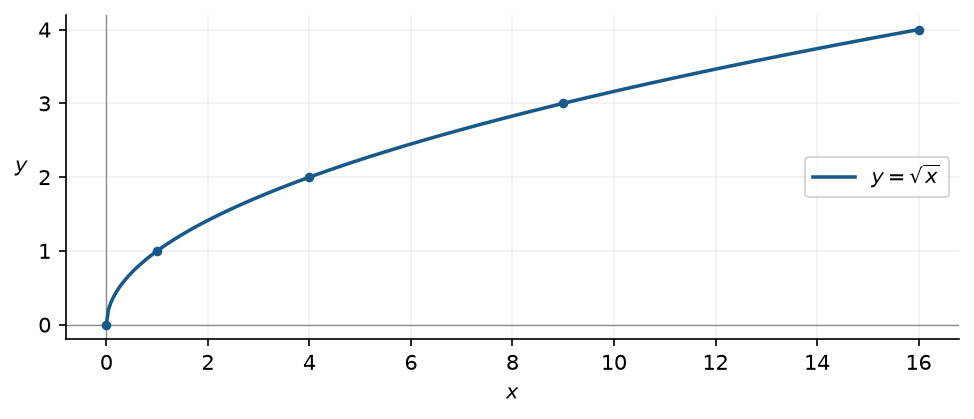
\includegraphics[width=.84\linewidth,height=.38\textheight,keepaspectratio]{figures/C03-EX071-5.png}\end{center}
{\small \field{关联知识}{F04 函数三种表示法、图象与读数（教材帮p.85、86、93、94 / PDF94、95、102、103）}
\field{方法与易错点}{把关键点与定义域一起标到图上，逐区间读交点和上下关系。 易错：将示意图预测当事实；把两曲线交点收进严格不等式；折线漏端点。}
\field{答案依据}{例题原解位置：湘教版教材p.71及题库原图；独立编写可编辑参考解答。答案册此部分主要收练习、习题，不伪造例题答案册位置。}}

\itemhead{p.72 练习 · 第1题（教材p.72）}{XJ-B1-C03-PR-P072-Y1158}
\label{XJ-B1-C03-PR-P072-Y1158}
{\footnotesize 湘教版教材p.72 / PDF第79页 / p.72 练习 / 第1题}
\field{原题}{学校要印刷一批资料，现要求纵向矩形纸面上、下各留 $4\,\mathrm{cm}$ 空白，左、右各留 $3\,\mathrm{cm}$ 空白，中间排版部分要求面积为 $432\,\mathrm{cm^2}$。写出纸张面积 $y$（$\mathrm{cm^2}$）与中间排版部分宽度 $x$（$\mathrm{cm}$）之间的函数解析式 $y=S(x)$，确定其定义域，再计算出 $S(8),S(12),S(24)$ 的值。}
\field{参考答案}{$S(x)=(x+6)(432/x+8)=8x+480+2592/x$，$x>0$；$S(8)=868,S(12)=792,S(24)=780$，单位为平方厘米。}
{\small \field{关联知识}{F03 函数求值、解析式与函数建模（教材帮p.80、87、88、89、90、131 / PDF89、96、97、98、99、140）；F02 定义域与原式限制（教材帮p.79、80、81 / PDF88、89、90）}
\field{方法与易错点}{标清每次输入和输出；按已知函数类型或代换关系建立等价方程。 易错：将 $f(x)$ 当成 $f	imes x$；复合顺序反；换元后沿用错误定义域。}
\field{答案依据}{答案册相关题组：PDF第19页（册内页18）；按当前题库原题逐项重算，不按旧版题号机械对套。}}

\itemhead{p.72 练习 · 第2题（教材p.72）}{XJ-B1-C03-PR-P072-Y1330}
\label{XJ-B1-C03-PR-P072-Y1330}
{\footnotesize 湘教版教材p.72 / PDF第79页 / p.72 练习 / 第2题}
\field{原题}{利用课本中关于水库蓄水量的列表作出由水深确定存水量的函数图象，并根据图象估计出水深为 $7\,\mathrm m$ 和 $18\,\mathrm m$ 时的存水量。
\par\textit{教材p.70被引用的数据：}
\begin{center}\begin{tabular}{c|rrrrrrr}\hline
最大水深 $H/\mathrm m$&5&10&15&20&25&30&35\\
存水量 $Q/(10^4\,\mathrm{m^3})$&20&40&90&160&275&437&650\\\hline
\end{tabular}\end{center}}
\field{参考答案}{在 $H$ 为横轴、$Q$ 为纵轴的坐标系中标出表内7点并用平滑趋势曲线连接。读图参考值分别约为 $28\times10^4$、$132\times10^4$ 立方米（若用相邻数据线性插值）。平滑作图可有差异，答案册示意图读数约25、140，均属估计，不能视为精确唯一值。}
\begin{center}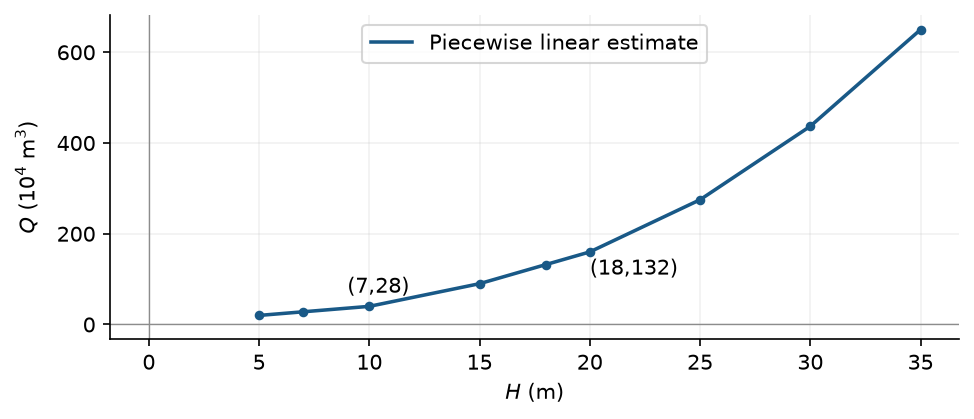
\includegraphics[width=.84\linewidth,height=.38\textheight,keepaspectratio]{figures/C03-PR072-2.png}\end{center}
图为相邻数据的线性插值示例，非唯一的真实库容曲线。\par
\field{核对说明}{读图估计非唯一：表内数据不能唯一确定中间函数值；保留答案册平滑曲线估计25、140，并给线性插值28、132及方法，均不当作精确值。}
{\small \field{关联知识}{F04 函数三种表示法、图象与读数（教材帮p.85、86、93、94 / PDF94、95、102、103）}
\field{方法与易错点}{把关键点与定义域一起标到图上，逐区间读交点和上下关系。 易错：将示意图预测当事实；把两曲线交点收进严格不等式；折线漏端点。}
\field{答案依据}{答案册相关题组：PDF第19页（册内页18）；按当前题库原题逐项重算，不按旧版题号机械对套。}}

\itemhead{p.72 练习 · 第3题（教材p.72）}{XJ-B1-C03-PR-P072-Y1416}
\label{XJ-B1-C03-PR-P072-Y1416}
{\footnotesize 湘教版教材p.72 / PDF第79页 / p.72 练习 / 第3题}
\field{原题}{画出函数 $f(x)=-x^2+2x+3$ 的图象，并根据图象回答下列问题：
\subq{1}比较 $f(0),f(1),f(3)$ 的大小；
\subq{2}若 $x_1<x_2<1$，比较 $f(x_1)$ 与 $f(x_2)$ 的大小；
\subq{3}求函数 $f(x)$ 的值域。}
\field{参考答案}{$f(x)=-(x-1)^2+4$，顶点 $(1,4)$，与 $x$ 轴交于 $(-1,0),(3,0)$。（1）$f(3)=0<f(0)=3<f(1)=4$；（2）$f(x_1)<f(x_2)$；（3）值域 $(-\infty,4]$。}
\begin{center}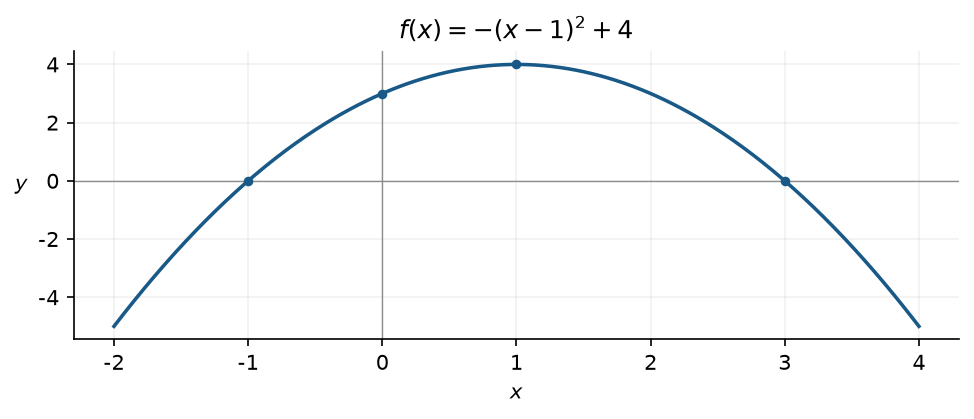
\includegraphics[width=.84\linewidth,height=.38\textheight,keepaspectratio]{figures/C03-PR072-3.png}\end{center}
\field{核对说明}{答案册方向笔误：答案册PDF19第3题第2问写f(x1)>f(x2)；在x1<x2<1时二次函数递增，正确为f(x1)<f(x2)。}
{\small \field{关联知识}{F04 函数三种表示法、图象与读数（教材帮p.85、86、93、94 / PDF94、95、102、103）；F05 单调性定义、证明与参数（教材帮p.97、98、100 / PDF106、107、109）；F06 最大值、最小值与值域（教材帮p.99、83、84 / PDF108、92、93）}
\field{方法与易错点}{把关键点与定义域一起标到图上，逐区间读交点和上下关系。 易错：将示意图预测当事实；把两曲线交点收进严格不等式；折线漏端点。}
\field{答案依据}{答案册相关题组：PDF第19页（册内页18）；按当前题库原题逐项重算，不按旧版题号机械对套。}}

\itemhead{数学实验 · 完整实验任务（教材p.73）}{XJ-B1-C03-LAB-P073-Y0145}
\label{XJ-B1-C03-LAB-P073-Y0145}
{\footnotesize 湘教版教材p.73 / PDF第80页 / 数学实验 / 完整实验任务}
\field{原题}{\textbf{用计算机作函数图象和列函数表}
\par 函数的图象能够帮助我们了解函数的性质。我们可以使用计算机技术，根据函数解析式和数据作出函数的图象。使用“超级画板”或其他具有类似功能的软件，在计算机上作函数的图象既快捷又准确。
\par 在右键菜单里单击“函数或参数方程曲线”，在出现的对话框里输入函数表达式“\texttt{x\textasciicircum(1/2)}”，参数范围取 0 到 10，点数取 101，单击“确定”，函数 $y=\sqrt x$ 的图象就出现了。
\bankfig{C03-LAB073}{0.68}
\par 用鼠标在曲线附近单击左键，曲线变色，表示计算机知道你选择了它。执行菜单命令“插入$\mid$表格”，屏幕上就出现了对应的函数表。
\par 这时表上的格子不够，可以用鼠标指着表格按右键，在右键菜单中单击“属性”，打开表格的属性设置对话框，在对话框下部把表格的行数改为 11，列数改为 20，单击“确定”即可。
\par\textit{原页中的软件结果表为操作示例，可在教材p.73核对；本条保留全部实验操作文字与数学表达式，不把软件结果表混作题目条件。}}
\field{参考答案}{实验核查：输入 $y=\sqrt x$，范围 $[0,10]$，101个等距点的横坐标为 $x_k=k/10$（$k=0,\ldots,100$），函数值为 $\sqrt{k/10}$。例如 $(0,0),(1,1),(4,2),(9,3),(10,\sqrt{10})$；图表应一一对应且无负横坐标，不以软件截图代替定义域判断。}
\begin{center}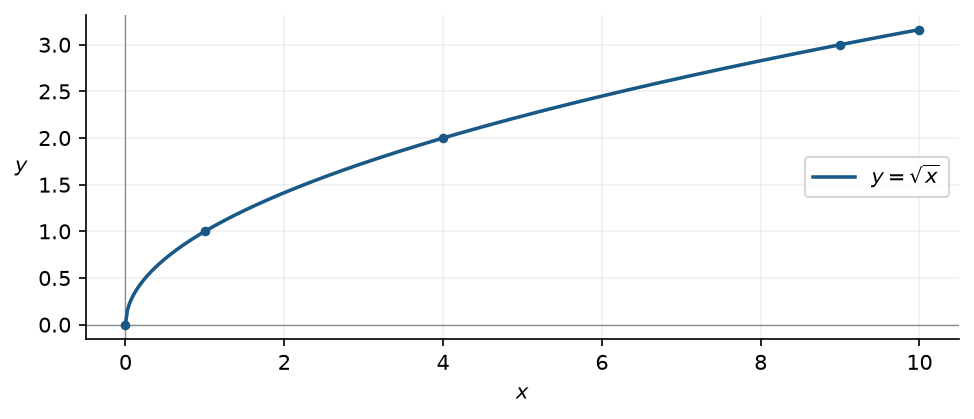
\includegraphics[width=.84\linewidth,height=.38\textheight,keepaspectratio]{figures/C03-LAB073.png}\end{center}
{\small \field{关联知识}{F04 函数三种表示法、图象与读数（教材帮p.85、86、93、94 / PDF94、95、102、103）}
\field{方法与易错点}{把关键点与定义域一起标到图上，逐区间读交点和上下关系。 易错：将示意图预测当事实；把两曲线交点收进严格不等式；折线漏端点。}
\field{答案依据}{答案册未提供本栏目的独立对应答案；依据原题、教材概念补写参考回应。开放性总结不设唯一数值答案。}}

\itemhead{3.1 例题 · 例题6（教材p.74）}{XJ-B1-C03-EX-P074-Y0394}
\label{XJ-B1-C03-EX-P074-Y0394}
{\footnotesize 湘教版教材p.74 / PDF第81页 / 3.1 例题 / 例题6}
\field{原题}{为推进生态优先、节约集约、绿色低碳发展，推动形成绿色低碳的生产方式和生活方式，某地采用分段计费的方法计算用户的电费：每月用电量不超过 $100\,\mathrm{kW\cdot h}$，按 $0.57$ 元/($\mathrm{kW\cdot h}$)计费；每月用电量超过 $100\,\mathrm{kW\cdot h}$，其中 $100\,\mathrm{kW\cdot h}$ 仍按原标准收费，超过部分按 $1.5$ 元/($\mathrm{kW\cdot h}$)计费。
\subq{1}设月用电 $x\,\mathrm{kW\cdot h}$，应交电费 $y$ 元，写出 $y$ 关于 $x$ 的函数解析式。
\subq{2}小赵家第一季度缴纳的电费情况如下表：
\begin{center}\begin{tabular}{c|rrrr}\hline
月份&1&2&3&合计\\
计费金额/元&114&75&45.6&234.6\\\hline
\end{tabular}\end{center}
问：小赵家第一季度共用电多少？}
\field{参考答案}{（1）$y=\begin{cases}0.57x,&0\le x\le100,\\1.5x-93,&x>100.\end{cases}$（2）各月用电138、112、80千瓦时，合计330千瓦时。须把超过100的部分单独计费。}
{\small \field{关联知识}{F07 分段函数、绝对值及分段应用（教材帮p.86、91、92、93 / PDF95、100、101、102）；F03 函数求值、解析式与函数建模（教材帮p.80、87、88、89、90、131 / PDF89、96、97、98、99、140）}
\field{方法与易错点}{先列转折点和各段条件，再建立分段式，检查衔接、定义域与值域。 易错：跨段套公式；超额部分按全量收费；绝对值去号漏区间。}
\field{答案依据}{例题原解位置：湘教版教材p.74及题库原图；独立编写可编辑参考解答。答案册此部分主要收练习、习题，不伪造例题答案册位置。}}

\itemhead{3.1 例题 · 例题7（教材p.75）}{XJ-B1-C03-EX-P075-Y0177}
\label{XJ-B1-C03-EX-P075-Y0177}
{\footnotesize 湘教版教材p.75 / PDF第82页 / 3.1 例题 / 例题7}
\field{原题}{画出函数 $f(x)=|x|$ 的图象，并求 $f(-3),f(3),f(-1),f(1)$ 的值。}
\field{参考答案}{$f(x)=\begin{cases}-x,&x<0,\\x,&x\ge0.\end{cases}$，图象为顶点 $(0,0)$ 的V形；四个值依次为3、3、1、1。}
\begin{center}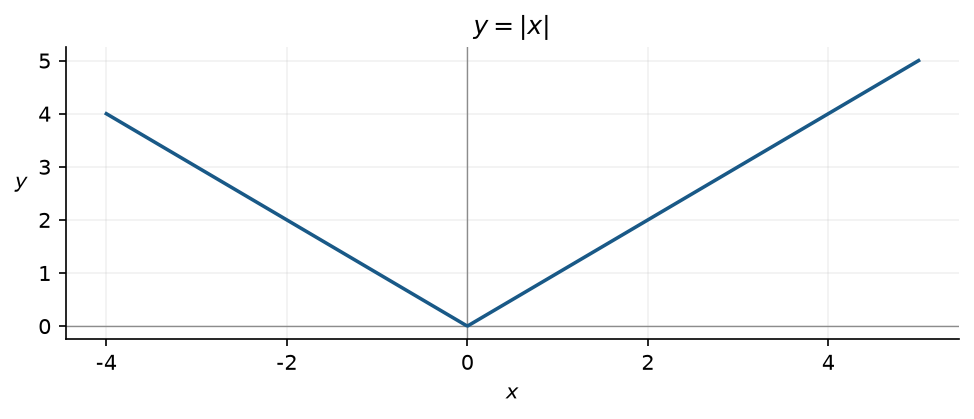
\includegraphics[width=.84\linewidth,height=.38\textheight,keepaspectratio]{figures/C03-EX075-7.png}\end{center}
{\small \field{关联知识}{F07 分段函数、绝对值及分段应用（教材帮p.86、91、92、93 / PDF95、100、101、102）；F04 函数三种表示法、图象与读数（教材帮p.85、86、93、94 / PDF94、95、102、103）}
\field{方法与易错点}{先列转折点和各段条件，再建立分段式，检查衔接、定义域与值域。 易错：跨段套公式；超额部分按全量收费；绝对值去号漏区间。}
\field{答案依据}{例题原解位置：湘教版教材p.75及题库原图；独立编写可编辑参考解答。答案册此部分主要收练习、习题，不伪造例题答案册位置。}}

\itemhead{3.1 例题 · 例题8（教材p.75）}{XJ-B1-C03-EX-P075-Y0639}
\label{XJ-B1-C03-EX-P075-Y0639}
{\footnotesize 湘教版教材p.75 / PDF第82页 / 3.1 例题 / 例题8}
\field{原题}{画出函数 $f(x)=|x-2|+|x+1|$ 的图象。}
\field{参考答案}{$f(x)=\begin{cases}1-2x,&x<-1,\\3,&-1\le x\le2,\\2x-1,&x>2.\end{cases}$，按两条射线与水平线段画图，转折点为 $(-1,3),(2,3)$，值域 $[3,+\infty)$。}
\begin{center}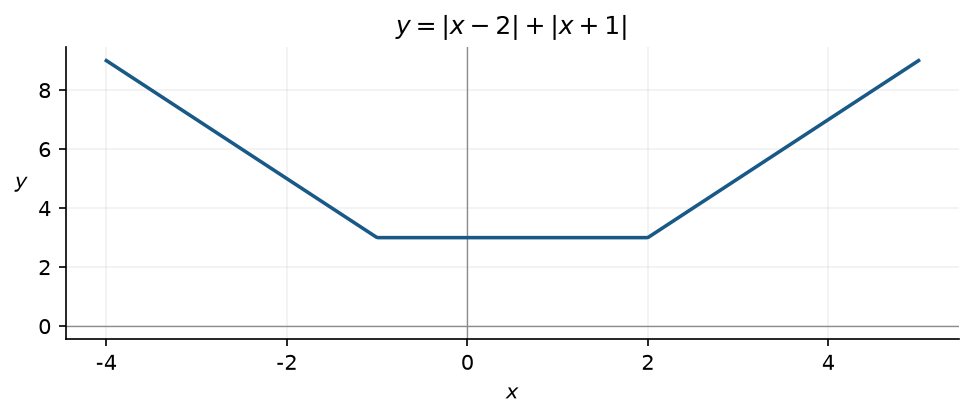
\includegraphics[width=.84\linewidth,height=.38\textheight,keepaspectratio]{figures/C03-EX075-8.png}\end{center}
{\small \field{关联知识}{F07 分段函数、绝对值及分段应用（教材帮p.86、91、92、93 / PDF95、100、101、102）；F04 函数三种表示法、图象与读数（教材帮p.85、86、93、94 / PDF94、95、102、103）}
\field{方法与易错点}{先列转折点和各段条件，再建立分段式，检查衔接、定义域与值域。 易错：跨段套公式；超额部分按全量收费；绝对值去号漏区间。}
\field{答案依据}{例题原解位置：湘教版教材p.75及题库原图；独立编写可编辑参考解答。答案册此部分主要收练习、习题，不伪造例题答案册位置。}}

\itemhead{p.76 练习 · 第1题（教材p.76）}{XJ-B1-C03-PR-P076-Y0217}
\label{XJ-B1-C03-PR-P076-Y0217}
{\footnotesize 湘教版教材p.76 / PDF第83页 / p.76 练习 / 第1题}
\field{原题}{作出下列函数的图象，并写出函数的值域：
\subq{1}$y=|x+3|$；
\subq{2}$y=|x-2|-|x+2|$。}
\field{参考答案}{（1）顶点 $(-3,0)$ 的V形图，值域 $[0,+\infty)$；（2）$f(x)=4$（$x\le-2$）、$-2x$（$-2<x<2$）、$-4$（$x\ge2$），值域 $[-4,4]$。}
\begin{center}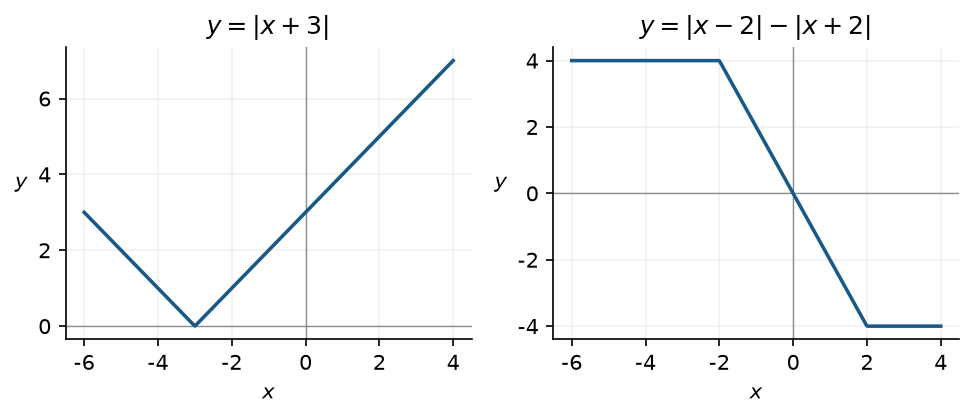
\includegraphics[width=.84\linewidth,height=.38\textheight,keepaspectratio]{figures/C03-PR076-1.png}\end{center}
{\small \field{关联知识}{F07 分段函数、绝对值及分段应用（教材帮p.86、91、92、93 / PDF95、100、101、102）；F04 函数三种表示法、图象与读数（教材帮p.85、86、93、94 / PDF94、95、102、103）}
\field{方法与易错点}{先列转折点和各段条件，再建立分段式，检查衔接、定义域与值域。 易错：跨段套公式；超额部分按全量收费；绝对值去号漏区间。}
\field{答案依据}{答案册相关题组：PDF第20页（册内页19）；按当前题库原题逐项重算，不按旧版题号机械对套。}}

\itemhead{p.76 练习 · 第2题（教材p.76）}{XJ-B1-C03-PR-P076-Y0364}
\label{XJ-B1-C03-PR-P076-Y0364}
{\footnotesize 湘教版教材p.76 / PDF第83页 / p.76 练习 / 第2题}
\field{原题}{已知函数 $f(x)=\begin{cases}|x|,&x<-1,\\\sqrt{1-x^2},&-1\le x\le1,\\1,&x>1.\end{cases}$
\subq{1}求 $f(3)+f(-3)f\left(\dfrac13\right)$ 的值；
\subq{2}若存在点 $x_0$，使得 $f(x_0)=1$，求实数 $x_0$ 的值。}
\field{参考答案}{（1）$1+2\sqrt2$；（2）$x_0\in\{0\}\cup(1,+\infty)$。左侧分段要求 $x<-1$，不能误收 $x=-1$。}
{\small \field{关联知识}{F07 分段函数、绝对值及分段应用（教材帮p.86、91、92、93 / PDF95、100、101、102）；F03 函数求值、解析式与函数建模（教材帮p.80、87、88、89、90、131 / PDF89、96、97、98、99、140）}
\field{方法与易错点}{先列转折点和各段条件，再建立分段式，检查衔接、定义域与值域。 易错：跨段套公式；超额部分按全量收费；绝对值去号漏区间。}
\field{答案依据}{答案册相关题组：PDF第20页（册内页19）；按当前题库原题逐项重算，不按旧版题号机械对套。}}

\itemhead{p.76 练习 · 第3题（教材p.76）}{XJ-B1-C03-PR-P076-Y0567}
\label{XJ-B1-C03-PR-P076-Y0567}
{\footnotesize 湘教版教材p.76 / PDF第83页 / p.76 练习 / 第3题}
\field{原题}{一个质点沿直线运动。质点由静止匀加速 $T\,\mathrm s$ 后速度达到 $8\,\mathrm{m/s}$，然后质点以恒定速度 $8\,\mathrm{m/s}$ 运动了 $5T\,\mathrm s$，之后质点在 $40\,\mathrm s$ 内匀减速到完全停下。
\subq{1}画出质点运动的速度-时间图象；
\subq{2}已知质点运动的总位移是 $600\,\mathrm m$，求 $T$ 的值；
\subq{3}画出质点运动的加速度-时间图象。}
\field{参考答案}{（1）$v(t)=8t/T$（$0\le t\le T$）、8（$T<t\le6T$）、$8-(t-6T)/5$（$6T<t\le6T+40$）；折线经过 $(0,0),(T,8),(6T,8),(6T+40,0)$。（2）面积给出 $44T+160=600$，故 $T=10$ s。（3）在三个运动阶段内部 $a=0.8,0,-0.2$（米每二次方秒）；理想模型在速度折点处不要求加速度存在。}
\begin{center}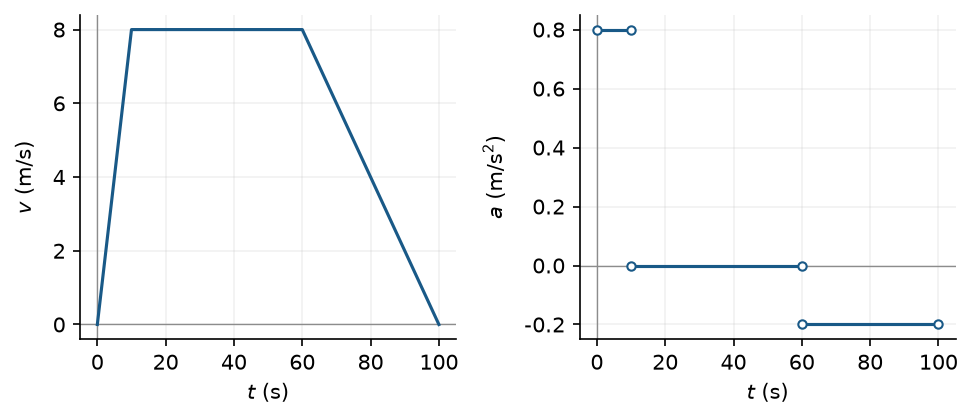
\includegraphics[width=.84\linewidth,height=.38\textheight,keepaspectratio]{figures/C03-PR076-3.png}\end{center}
{\small \field{关联知识}{F07 分段函数、绝对值及分段应用（教材帮p.86、91、92、93 / PDF95、100、101、102）；F04 函数三种表示法、图象与读数（教材帮p.85、86、93、94 / PDF94、95、102、103）}
\field{方法与易错点}{先列转折点和各段条件，再建立分段式，检查衔接、定义域与值域。 易错：跨段套公式；超额部分按全量收费；绝对值去号漏区间。}
\field{答案依据}{答案册相关题组：PDF第20页（册内页19）；按当前题库原题逐项重算，不按旧版题号机械对套。}}

\itemhead{习题3.1 · 第1题（教材p.76）}{XJ-B1-C03-HW-P076-Y1136}
\label{XJ-B1-C03-HW-P076-Y1136}
{\footnotesize 湘教版教材p.76 / PDF第83页 / 习题3.1 / 第1题}
\field{原题}{设集合 $M=\{x\mid0\le x\le2\}$，$N=\{y\mid0\le y\le2\}$，那么下列四个图形中，能表示集合 $M$ 到集合 $N$ 的函数关系的有（\quad）
\bankfig{C03-HW076}{0.92}
\choice{A}\textcircled{1}\textcircled{2}\textcircled{3}\textcircled{4}
\choice{B}\textcircled{1}\textcircled{2}\textcircled{3}
\choice{C}\textcircled{2}\textcircled{3}
\choice{D}\textcircled{2}}
\field{参考答案}{C。只有图\textcircled{2}、\textcircled{3}使每个 $x\in[0,2]$ 都恰有一个 $[0,2]$ 内的函数值。}
{\small \field{关联知识}{F01 函数本质、构成要素与相同函数（教材帮p.77、78 / PDF86、87）；F04 函数三种表示法、图象与读数（教材帮p.85、86、93、94 / PDF94、95、102、103）}
\field{方法与易错点}{逐一核对每个允许输入是否有且仅有一个合乎目标集合的输出。 易错：把值域直接当作目标集合；只看解析式外观；认为常函数不是函数。}
\field{答案依据}{答案册相关题组：PDF第20、21、22页（册内页19、20、21）；按当前题库原题逐项重算，不按旧版题号机械对套。}}

\itemhead{习题3.1 · 第2题（教材p.76）}{XJ-B1-C03-HW-P076-Y1523}
\label{XJ-B1-C03-HW-P076-Y1523}
{\footnotesize 湘教版教材p.76 / PDF第83页 / 习题3.1 / 第2题}
\field{原题}{已知定义域为 $\mathbb R$ 的函数 $f(x)=2x^2-3$ 和 $g(x)=4x$，求下列各式的值：
\[f(g(-1)),\quad g(f(-1)),\quad f(f(-2)),\quad g(g(-2)).\]}
\field{参考答案}{依次为29、$-4$、47、$-32$。}
{\small \field{关联知识}{F03 函数求值、解析式与函数建模（教材帮p.80、87、88、89、90、131 / PDF89、96、97、98、99、140）}
\field{方法与易错点}{标清每次输入和输出；按已知函数类型或代换关系建立等价方程。 易错：将 $f(x)$ 当成 $f	imes x$；复合顺序反；换元后沿用错误定义域。}
\field{答案依据}{答案册相关题组：PDF第20、21、22页（册内页19、20、21）；按当前题库原题逐项重算，不按旧版题号机械对套。}}

\itemhead{习题3.1 · 第3题（教材p.77）}{XJ-B1-C03-HW-P077-Y0228}
\label{XJ-B1-C03-HW-P077-Y0228}
{\footnotesize 湘教版教材p.77 / PDF第84页 / 习题3.1 / 第3题}
\field{原题}{已知函数 $f(x)=\dfrac x{x+1}$，求 $f(1)+f(2)+f(3)+f\left(\dfrac12\right)+f\left(\dfrac13\right)$ 的值。}
\field{参考答案}{$5/2$。$f(2)+f(1/2)=1$，$f(3)+f(1/3)=1$，另有 $f(1)=1/2$；即 $1/2+2/3+3/4+1/3+1/4=5/2$。}
{\small \field{关联知识}{F03 函数求值、解析式与函数建模（教材帮p.80、87、88、89、90、131 / PDF89、96、97、98、99、140）}
\field{方法与易错点}{标清每次输入和输出；按已知函数类型或代换关系建立等价方程。 易错：将 $f(x)$ 当成 $f	imes x$；复合顺序反；换元后沿用错误定义域。}
\field{答案依据}{答案册相关题组：PDF第20、21、22页（册内页19、20、21）；按当前题库原题逐项重算，不按旧版题号机械对套。}}

\itemhead{习题3.1 · 第4题（教材p.77）}{XJ-B1-C03-HW-P077-Y0286}
\label{XJ-B1-C03-HW-P077-Y0286}
{\footnotesize 湘教版教材p.77 / PDF第84页 / 习题3.1 / 第4题}
\field{原题}{求下列函数的定义域：
\subq{1}$y=\dfrac{\sqrt{x+1}}{x^2+2x-3}$；
\subq{2}$y=\dfrac{x+4}{x^3-4x}$。}
\field{参考答案}{（1）$[-1,1)\cup(1,+\infty)$；（2）$\mathbb R\setminus\{-2,0,2\}$。约去因子不能恢复原式排除的点。}
{\small \field{关联知识}{F02 定义域与原式限制（教材帮p.79、80、81 / PDF88、89、90）}
\field{方法与易错点}{按原式逐项列条件后求交集，不先约分再判断。 易错：遗漏分母禁点；将函数值范围错当自变量范围；把退化矩形算入实际定义域。}
\field{答案依据}{答案册相关题组：PDF第20、21、22页（册内页19、20、21）；按当前题库原题逐项重算，不按旧版题号机械对套。}}

\itemhead{习题3.1 · 第5题（教材p.77）}{XJ-B1-C03-HW-P077-Y0403}
\label{XJ-B1-C03-HW-P077-Y0403}
{\footnotesize 湘教版教材p.77 / PDF第84页 / 习题3.1 / 第5题}
\field{原题}{下列各组函数中，表示同一个函数的是（\quad）
\choice{A}$y=x-1$ 和 $y=\dfrac{x^2-1}{x+1}$
\choice{B}$y=x^0$ 和 $y=1$
\choice{C}$y=x^2$ 和 $y=(x+1)^2$
\choice{D}$y=\dfrac{(\sqrt x)^2}x$ 和 $y=\dfrac x{(\sqrt x)^2}$}
\field{参考答案}{D。两函数都在 $(0,+\infty)$ 上恒为1。B项 $x^0$ 还要求 $x\ne0$。}
{\small \field{关联知识}{F01 函数本质、构成要素与相同函数（教材帮p.77、78 / PDF86、87）；F02 定义域与原式限制（教材帮p.79、80、81 / PDF88、89、90）}
\field{方法与易错点}{逐一核对每个允许输入是否有且仅有一个合乎目标集合的输出。 易错：把值域直接当作目标集合；只看解析式外观；认为常函数不是函数。}
\field{答案依据}{答案册相关题组：PDF第20、21、22页（册内页19、20、21）；按当前题库原题逐项重算，不按旧版题号机械对套。}}

\itemhead{习题3.1 · 第6题（教材p.77）}{XJ-B1-C03-HW-P077-Y0601}
\label{XJ-B1-C03-HW-P077-Y0601}
{\footnotesize 湘教版教材p.77 / PDF第84页 / 习题3.1 / 第6题}
\field{原题}{作出下列函数的图象，并说出函数的定义域、值域。
\subq{1}$y=3x^2-5x+2$；
\subq{2}$y=|x-1|$。}
\field{参考答案}{（1）$y=3(x-5/6)^2-1/12$，定义域 $\mathbb R$、值域 $[-1/12,+\infty)$，顶点 $(5/6,-1/12)$；（2）V形图顶点 $(1,0)$，定义域 $\mathbb R$、值域 $[0,+\infty)$。}
\begin{center}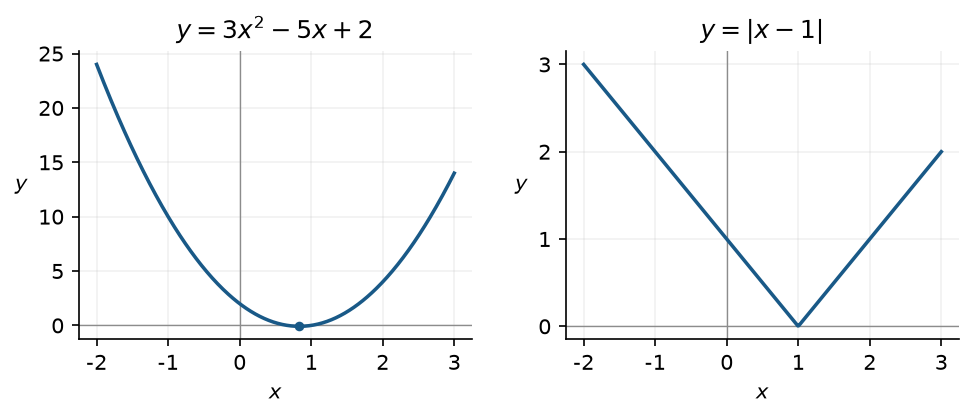
\includegraphics[width=.84\linewidth,height=.38\textheight,keepaspectratio]{figures/C03-HW077-6.png}\end{center}
{\small \field{关联知识}{F04 函数三种表示法、图象与读数（教材帮p.85、86、93、94 / PDF94、95、102、103）；F06 最大值、最小值与值域（教材帮p.99、83、84 / PDF108、92、93）}
\field{方法与易错点}{把关键点与定义域一起标到图上，逐区间读交点和上下关系。 易错：将示意图预测当事实；把两曲线交点收进严格不等式；折线漏端点。}
\field{答案依据}{答案册相关题组：PDF第20、21、22页（册内页19、20、21）；按当前题库原题逐项重算，不按旧版题号机械对套。}}

\itemhead{习题3.1 · 第7题（教材p.77）}{XJ-B1-C03-HW-P077-Y0687}
\label{XJ-B1-C03-HW-P077-Y0687}
{\footnotesize 湘教版教材p.77 / PDF第84页 / 习题3.1 / 第7题}
\field{原题}{已知圆 $O$ 的直径为 4，将该圆的内接矩形 $ABCD$（顶点都在圆上）的面积表示为它的一边 $AB$ 的长 $x$ 的函数 $f(x)$，并求出其定义域。}
\field{参考答案}{$f(x)=x\sqrt{16-x^2}$，$x\in(0,4)$。矩形不能退化，0、4都不属于定义域。}
{\small \field{关联知识}{F03 函数求值、解析式与函数建模（教材帮p.80、87、88、89、90、131 / PDF89、96、97、98、99、140）；F02 定义域与原式限制（教材帮p.79、80、81 / PDF88、89、90）}
\field{方法与易错点}{标清每次输入和输出；按已知函数类型或代换关系建立等价方程。 易错：将 $f(x)$ 当成 $f	imes x$；复合顺序反；换元后沿用错误定义域。}
\field{答案依据}{答案册相关题组：PDF第20、21、22页（册内页19、20、21）；按当前题库原题逐项重算，不按旧版题号机械对套。}}

\itemhead{习题3.1 · 第8题（教材p.77）}{XJ-B1-C03-HW-P077-Y0773}
\label{XJ-B1-C03-HW-P077-Y0773}
{\footnotesize 湘教版教材p.77 / PDF第84页 / 习题3.1 / 第8题}
\field{原题}{函数 $f(x)$ 与 $g(x)$ 的定义域均为 $[m,n]$，它们的图象如下图所示，则不等式 $f(x)>g(x)$ 的解集是（\quad）
\bankfig{C03-HW077-08}{0.55}
\choice{A}$[m,a)\cup(b,e)$
\choice{B}$(a,c)\cup(e,n]$
\choice{C}$[m,a]\cup(b,c)$
\choice{D}$(a,b)\cup(c,e)$}
\field{参考答案}{A，解集为 $[m,a)\cup(b,e)$；两曲线交点处不取等号。}
{\small \field{关联知识}{F04 函数三种表示法、图象与读数（教材帮p.85、86、93、94 / PDF94、95、102、103）}
\field{方法与易错点}{把关键点与定义域一起标到图上，逐区间读交点和上下关系。 易错：将示意图预测当事实；把两曲线交点收进严格不等式；折线漏端点。}
\field{答案依据}{答案册相关题组：PDF第20、21、22页（册内页19、20、21）；按当前题库原题逐项重算，不按旧版题号机械对套。}}

\itemhead{习题3.1 · 第9题（教材p.77）}{XJ-B1-C03-HW-P077-Y1227}
\label{XJ-B1-C03-HW-P077-Y1227}
{\footnotesize 湘教版教材p.77 / PDF第84页 / 习题3.1 / 第9题}
\field{原题}{某农场种植西红柿，由历年市场行情得知，从 2 月 1 日起的 300 天内，西红柿市场售价与上市时间的关系可用如下图所示的一条折线表示，写出市场售价与时间的函数解析式 $P=f(t)$。
\bankfig{C03-HW077-09}{0.48}}
\field{参考答案}{$P(t)=\begin{cases}3-t/100,&0\le t\le200,\\t/50-3,&200<t\le300.\end{cases}$，单位元/kg。若 $t$ 只表示整数天，另取 $t\in\mathbb Z$；两段在200处都给出1。}
{\small \field{关联知识}{F07 分段函数、绝对值及分段应用（教材帮p.86、91、92、93 / PDF95、100、101、102）；F03 函数求值、解析式与函数建模（教材帮p.80、87、88、89、90、131 / PDF89、96、97、98、99、140）}
\field{方法与易错点}{先列转折点和各段条件，再建立分段式，检查衔接、定义域与值域。 易错：跨段套公式；超额部分按全量收费；绝对值去号漏区间。}
\field{答案依据}{答案册相关题组：PDF第20、21、22页（册内页19、20、21）；按当前题库原题逐项重算，不按旧版题号机械对套。}}

\itemhead{习题3.1 · 第10题（教材p.77）}{XJ-B1-C03-HW-P077-Y1356}
\label{XJ-B1-C03-HW-P077-Y1356}
{\footnotesize 湘教版教材p.77 / PDF第84页 / 习题3.1 / 第10题}
\field{原题}{滑雪运动员以恒定加速度沿着笔直的雪道向下滑。在 $t=0$ 时刻，他以 $6\,\mathrm{m/s}$ 的速度经过点 $A$，然后加速下滑直到以 $15\,\mathrm{m/s}$ 的速度经过点 $B$。在 $B$ 点，雪道开始变平，他从 $B$ 点开始以恒定速度 $15\,\mathrm{m/s}$ 滑到 $C$ 点。已知 $A,C$ 之间的路程是 $615\,\mathrm m$，他从 $B$ 点滑到 $C$ 点用了 $20\,\mathrm s$。
\subq{1}求出 $A,B$ 之间的路程；
\subq{2}求该运动员从 $A$ 滑到 $B$ 的时间；
\subq{3}画出该运动员滑雪的速度-时间图象。}
\field{参考答案}{（1）$AB=615-15\times20=315$ m；（2）$t_{AB}=315/[(6+15)/2]=30$ s；（3）图象为 $(0,6)$ 到 $(30,15)$ 的线段，再连接 $(50,15)$。即 $v=6+0.3t$（$0\le t\le30$）、$v=15$（$30<t\le50$）。}
\begin{center}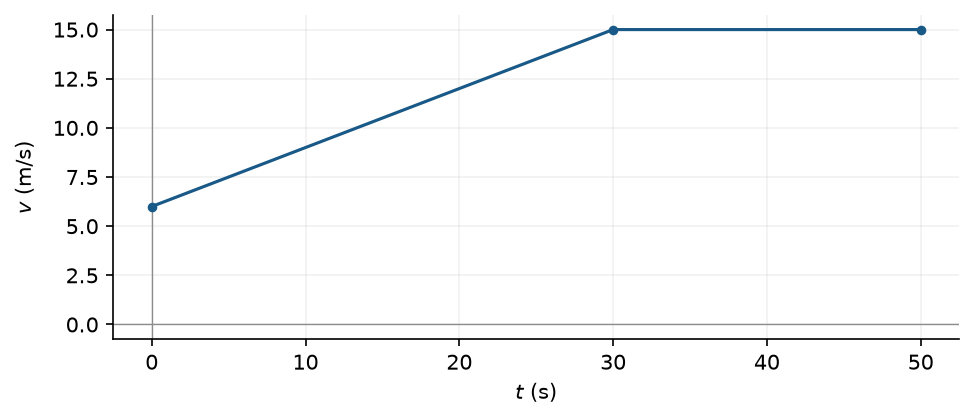
\includegraphics[width=.84\linewidth,height=.38\textheight,keepaspectratio]{figures/C03-HW077-10.png}\end{center}
{\small \field{关联知识}{F07 分段函数、绝对值及分段应用（教材帮p.86、91、92、93 / PDF95、100、101、102）；F04 函数三种表示法、图象与读数（教材帮p.85、86、93、94 / PDF94、95、102、103）}
\field{方法与易错点}{先列转折点和各段条件，再建立分段式，检查衔接、定义域与值域。 易错：跨段套公式；超额部分按全量收费；绝对值去号漏区间。}
\field{答案依据}{答案册相关题组：PDF第20、21、22页（册内页19、20、21）；按当前题库原题逐项重算，不按旧版题号机械对套。}}

\itemhead{习题3.1 · 第11题（教材p.78）}{XJ-B1-C03-HW-P078-Y0473}
\label{XJ-B1-C03-HW-P078-Y0473}
{\footnotesize 湘教版教材p.78 / PDF第85页 / 习题3.1 / 第11题}
\field{原题}{已知函数 $f(x),g(x)$ 分别由下表给出：
\begin{center}\begin{tabular}{c|rrr}\hline
$x$&1&2&3\\$f(x)$&1&3&1\\$g(x)$&3&2&1\\\hline
\end{tabular}\end{center}
则 $f(g(1))$ 的值为\blank；满足 $f(g(x))>g(f(x))$ 的 $x$ 的值是\blank。}
\field{参考答案}{两空为1、2。逐个代入 $x\in\{1,2,3\}$ 核对，只有 $x=2$ 满足不等式。}
{\small \field{关联知识}{F03 函数求值、解析式与函数建模（教材帮p.80、87、88、89、90、131 / PDF89、96、97、98、99、140）}
\field{方法与易错点}{标清每次输入和输出；按已知函数类型或代换关系建立等价方程。 易错：将 $f(x)$ 当成 $f	imes x$；复合顺序反；换元后沿用错误定义域。}
\field{答案依据}{答案册相关题组：PDF第20、21、22页（册内页19、20、21）；按当前题库原题逐项重算，不按旧版题号机械对套。}}

\itemhead{习题3.1 · 第12题（教材p.78）}{XJ-B1-C03-HW-P078-Y0673}
\label{XJ-B1-C03-HW-P078-Y0673}
{\footnotesize 湘教版教材p.78 / PDF第85页 / 习题3.1 / 第12题}
\field{原题}{已知函数 $f(x)$ 对任意 $t\in\mathbb R$ 满足等式 $f(1-t)=1+t^2$，求 $f(x)$。}
\field{参考答案}{置 $x=1-t$，得 $f(x)=1+(1-x)^2=x^2-2x+2$，$x\in\mathbb R$。}
{\small \field{关联知识}{F03 函数求值、解析式与函数建模（教材帮p.80、87、88、89、90、131 / PDF89、96、97、98、99、140）}
\field{方法与易错点}{标清每次输入和输出；按已知函数类型或代换关系建立等价方程。 易错：将 $f(x)$ 当成 $f	imes x$；复合顺序反；换元后沿用错误定义域。}
\field{答案依据}{答案册相关题组：PDF第20、21、22页（册内页19、20、21）；按当前题库原题逐项重算，不按旧版题号机械对套。}}

\itemhead{习题3.1 · 第13题（教材p.78）}{XJ-B1-C03-HW-P078-Y0717}
\label{XJ-B1-C03-HW-P078-Y0717}
{\footnotesize 湘教版教材p.78 / PDF第85页 / 习题3.1 / 第13题}
\field{原题}{已知函数 $f(x)$ 的定义域为 $\mathbb R_+$，且满足 $f(xy)=f(x)+f(y)$，若 $f(27)=1$，求 $f(\sqrt3)$ 的值。}
\field{参考答案}{$f(\sqrt3)=1/6$。$f(27)=3f(3)=1$，$f(3)=2f(\sqrt3)$。不需要引入对数函数。}
{\small \field{关联知识}{F03 函数求值、解析式与函数建模（教材帮p.80、87、88、89、90、131 / PDF89、96、97、98、99、140）}
\field{方法与易错点}{标清每次输入和输出；按已知函数类型或代换关系建立等价方程。 易错：将 $f(x)$ 当成 $f	imes x$；复合顺序反；换元后沿用错误定义域。}
\field{答案依据}{答案册相关题组：PDF第20、21、22页（册内页19、20、21）；按当前题库原题逐项重算，不按旧版题号机械对套。}}

\itemhead{习题3.1 · 第14题（教材p.78）}{XJ-B1-C03-HW-P078-Y0808}
\label{XJ-B1-C03-HW-P078-Y0808}
{\footnotesize 湘教版教材p.78 / PDF第85页 / 习题3.1 / 第14题}
\field{原题}{如图，函数 $f(x)$ 的图象是折线段 $ABC$，其中点 $A,B,C$ 的坐标分别为 $(0,4),(2,0),(6,4)$，求 $f(f(f(2)))$ 的值。
\bankfig{C03-HW078-14}{0.4}}
\field{参考答案}{$f(2)=0,f(0)=4,f(4)=2$，故 $f(f(f(2)))=2$。}
{\small \field{关联知识}{F03 函数求值、解析式与函数建模（教材帮p.80、87、88、89、90、131 / PDF89、96、97、98、99、140）；F04 函数三种表示法、图象与读数（教材帮p.85、86、93、94 / PDF94、95、102、103）}
\field{方法与易错点}{标清每次输入和输出；按已知函数类型或代换关系建立等价方程。 易错：将 $f(x)$ 当成 $f	imes x$；复合顺序反；换元后沿用错误定义域。}
\field{答案依据}{答案册相关题组：PDF第20、21、22页（册内页19、20、21）；按当前题库原题逐项重算，不按旧版题号机械对套。}}

\itemhead{习题3.1 · 第15题（教材p.78）}{XJ-B1-C03-HW-P078-Y1137}
\label{XJ-B1-C03-HW-P078-Y1137}
{\footnotesize 湘教版教材p.78 / PDF第85页 / 习题3.1 / 第15题}
\field{原题}{如图，四边形 $ABCD$ 是边长为 4 的正方形，一个动点 $P$ 从点 $A$ 出发，沿着边 $AB\to BC\to CD\to DA$ 运动，返回到点 $A$ 后停止运动，设点 $P$ 走过的路程为 $x$。
\bankfig{C03-HW078-15}{0.36}
\subq{1}将线段 $AP$ 的长度表示成 $x$ 的函数 $f_1(x)$；
\subq{2}设点 $O$ 是正方形 $ABCD$ 的中心，当点 $A,O,P$ 三点不共线时，将 $\triangle AOP$ 的面积表示成 $x$ 的函数 $f_2(x)$。}
\field{参考答案}{（1）$f_1(x)=x$（$0\le x\le4$）、$\sqrt{16+(x-4)^2}$（$4<x\le8$）、$\sqrt{16+(12-x)^2}$（$8<x\le12$）、$16-x$（$12<x\le16$）。（2）$f_2(x)=x$（$0<x\le4$）、$8-x$（$4<x<8$）、$x-8$（$8<x\le12$）、$16-x$（$12<x<16$）；定义域为 $(0,8)\cup(8,16)$，必须排除三点共线的0、8、16。}
\field{核对说明}{定义域核验：三角形面积函数须排除A、O、P共线的路程0、8、16，不能把退化三角形包括进原问题。}
{\small \field{关联知识}{F07 分段函数、绝对值及分段应用（教材帮p.86、91、92、93 / PDF95、100、101、102）；F03 函数求值、解析式与函数建模（教材帮p.80、87、88、89、90、131 / PDF89、96、97、98、99、140）}
\field{方法与易错点}{先列转折点和各段条件，再建立分段式，检查衔接、定义域与值域。 易错：跨段套公式；超额部分按全量收费；绝对值去号漏区间。}
\field{答案依据}{答案册相关题组：PDF第20、21、22页（册内页19、20、21）；按当前题库原题逐项重算，不按旧版题号机械对套。}}

\itemhead{习题3.1 · 第16题（教材p.78）}{XJ-B1-C03-HW-P078-Y1352}
\label{XJ-B1-C03-HW-P078-Y1352}
{\footnotesize 湘教版教材p.78 / PDF第85页 / 习题3.1 / 第16题}
\field{原题}{设函数 $\operatorname{sign}(x)$ 的定义为 $\operatorname{sign}(x)=\begin{cases}0,&x\le0,\\1,&x>0.\end{cases}$
\subq{1}画出该函数的图象；
\subq{2}探索利用函数 $\operatorname{sign}(x)$ 把分段函数写成一个解析式的方法，并具体尝试用一个解析式来写出上面第 9 题中的函数。
\par\textit{引用定位：习题3.1第9题，教材p.77（西红柿价格与上市时间折线图），对应题库条目 XJ-B1-C03-HW-P077-Y1227。}}
\field{参考答案}{（1）$x\le0$ 时画水平线 $y=0$，$(0,0)$ 实心；$x>0$ 时画 $y=1$，$(0,1)$ 空心。（2）第9题可写为 $P(t)=3-t/100+(3t/100-6)\operatorname{sign}(t-200)$，$0\le t\le300$。此处必须使用题目定义的0、1阶跃函数，不能套用通常的正负号函数。}
\begin{center}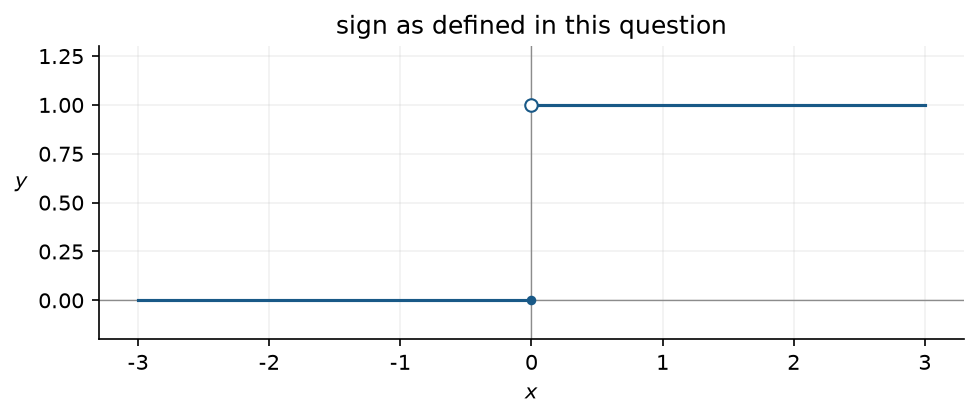
\includegraphics[width=.84\linewidth,height=.38\textheight,keepaspectratio]{figures/C03-HW078-16.png}\end{center}
\field{核对说明}{特殊定义提醒：本题sign为0/1阶跃函数，按其定义组织表达式；原题200处需检验，不能直接用常见的-1/0/1符号函数。}
{\small \field{关联知识}{F07 分段函数、绝对值及分段应用（教材帮p.86、91、92、93 / PDF95、100、101、102）}
\field{方法与易错点}{先列转折点和各段条件，再建立分段式，检查衔接、定义域与值域。 易错：跨段套公式；超额部分按全量收费；绝对值去号漏区间。}
\field{答案依据}{答案册相关题组：PDF第20、21、22页（册内页19、20、21）；按当前题库原题逐项重算，不按旧版题号机械对套。}}

\itemhead{3.2 思考 · 未编号题组（教材p.79）}{XJ-B1-C03-TH-P079-Y0868}
\label{XJ-B1-C03-TH-P079-Y0868}
{\footnotesize 湘教版教材p.79 / PDF第86页 / 3.2 思考 / 未编号题组}
\field{原题}{图 3.2-1 是湖北省武汉市某年 11 月 22 日 16 时到 23 日 16 时这 24 个小时内的气温变化图。该曲线给出了时间与气温间的函数关系。你能从中看出它的变化趋势和最高（或最低）温度吗？
\bankfig{C03-TH079}{0.78}}
\field{参考答案}{图中总体先下降后回升，期间有小幅波动；最低约 $11\,{}^\circ\mathrm C$（0时及3—4时附近），最高为次日16时约 $22.3\,{}^\circ\mathrm C$。不能把总体趋势说成全程单调。}
{\small \field{关联知识}{F04 函数三种表示法、图象与读数（教材帮p.85、86、93、94 / PDF94、95、102、103）；F05 单调性定义、证明与参数（教材帮p.97、98、100 / PDF106、107、109）；F06 最大值、最小值与值域（教材帮p.99、83、84 / PDF108、92、93）}
\field{方法与易错点}{把关键点与定义域一起标到图上，逐区间读交点和上下关系。 易错：将示意图预测当事实；把两曲线交点收进严格不等式；折线漏端点。}
\field{答案依据}{答案册未提供本栏目的独立对应答案；依据原题、教材概念补写参考回应。开放性总结不设唯一数值答案。}}

\itemhead{3.2 思考 · 未编号题组（教材p.81）}{XJ-B1-C03-TH-P081-Y0178}
\label{XJ-B1-C03-TH-P081-Y0178}
{\footnotesize 湘教版教材p.81 / PDF第88页 / 3.2 思考 / 未编号题组}
\field{原题}{怎样利用函数的解析式判断函数的单调性？}
\field{参考答案}{在指定区间内任取 $x_1<x_2$，作差 $f(x_2)-f(x_1)$；若恒正则递增，恒负则递减。论证必须覆盖区间内任意两点，不能仅列几个数值。}
{\small \field{关联知识}{F05 单调性定义、证明与参数（教材帮p.97、98、100 / PDF106、107、109）}
\field{方法与易错点}{用定义比较任意两值，或依据已知图象性质；含参时使指定区间被相应单调区间覆盖。 易错：用有限采样代替证明；把分离半轴合并；漏跨零点情形。}
\field{答案依据}{答案册未提供本栏目的独立对应答案；依据原题、教材概念补写参考回应。开放性总结不设唯一数值答案。}}

\itemhead{3.2 例题 · 例题1（教材p.81）}{XJ-B1-C03-EX-P081-Y0375}
\label{XJ-B1-C03-EX-P081-Y0375}
{\footnotesize 湘教版教材p.81 / PDF第88页 / 3.2 例题 / 例题1}
\field{原题}{已知函数 $f(x)=3x+b\ (x\in\mathbb R)$，判断该函数的单调性。}
\field{参考答案}{在 $\mathbb R$ 上单调递增，因为 $f(x_2)-f(x_1)=3(x_2-x_1)>0$。}
{\small \field{关联知识}{F05 单调性定义、证明与参数（教材帮p.97、98、100 / PDF106、107、109）}
\field{方法与易错点}{用定义比较任意两值，或依据已知图象性质；含参时使指定区间被相应单调区间覆盖。 易错：用有限采样代替证明；把分离半轴合并；漏跨零点情形。}
\field{答案依据}{例题原解位置：湘教版教材p.81及题库原图；独立编写可编辑参考解答。答案册此部分主要收练习、习题，不伪造例题答案册位置。}}

\itemhead{3.2 例题 · 例题2（教材p.81）}{XJ-B1-C03-EX-P081-Y1313}
\label{XJ-B1-C03-EX-P081-Y1313}
{\footnotesize 湘教版教材p.81 / PDF第88页 / 3.2 例题 / 例题2}
\field{原题}{证明函数 $f(x)=x+\dfrac1x\ (x>0)$ 在区间 $(0,1]$ 上单调递减，在区间 $[1,+\infty)$ 上单调递增，并指出函数在区间 $(0,+\infty)$ 上的最值点和最值。}
\field{参考答案}{$f(x_2)-f(x_1)=(x_2-x_1)(1-1/(x_1x_2))$；在 $(0,1]$ 内为负，在 $[1,+\infty)$ 内为正。最小值2在 $x=1$ 取得，无最大值。}
{\small \field{关联知识}{F05 单调性定义、证明与参数（教材帮p.97、98、100 / PDF106、107、109）；F06 最大值、最小值与值域（教材帮p.99、83、84 / PDF108、92、93）}
\field{方法与易错点}{用定义比较任意两值，或依据已知图象性质；含参时使指定区间被相应单调区间覆盖。 易错：用有限采样代替证明；把分离半轴合并；漏跨零点情形。}
\field{答案依据}{例题原解位置：湘教版教材p.81及题库原图；独立编写可编辑参考解答。答案册此部分主要收练习、习题，不伪造例题答案册位置。}}

\itemhead{3.2 例题 · 例题3（教材p.82）}{XJ-B1-C03-EX-P082-Y0618}
\label{XJ-B1-C03-EX-P082-Y0618}
{\footnotesize 湘教版教材p.82 / PDF第89页 / 3.2 例题 / 例题3}
\field{原题}{若函数 $f(x)=x^2+2(a-1)x+2$ 在区间 $(-\infty,4)$ 上单调递减，求实数 $a$ 的取值范围。}
\field{参考答案}{对称轴为 $x=1-a$，需 $1-a\ge4$，故 $a\le-3$。}
{\small \field{关联知识}{F05 单调性定义、证明与参数（教材帮p.97、98、100 / PDF106、107、109）；Q01 二次函数、零点、判别式与根系关系（教材帮p.65 / PDF74）}
\field{方法与易错点}{用定义比较任意两值，或依据已知图象性质；含参时使指定区间被相应单调区间覆盖。 易错：用有限采样代替证明；把分离半轴合并；漏跨零点情形。}
\field{答案依据}{例题原解位置：湘教版教材p.82及题库原图；独立编写可编辑参考解答。答案册此部分主要收练习、习题，不伪造例题答案册位置。}}

\itemhead{p.82 练习 · 第1题（教材p.82）}{XJ-B1-C03-PR-P082-Y1064}
\label{XJ-B1-C03-PR-P082-Y1064}
{\footnotesize 湘教版教材p.82 / PDF第89页 / p.82 练习 / 第1题}
\field{原题}{\subq{1}若函数 $f(x)$ 在定义域 $[a,b]$ 上单调递减，则 $f(x)$ 的最大值是多少？
\subq{2}若函数 $f(x)$ 在区间 $[a,u]$ 上单调递减，在区间 $[u,b]$ 上单调递增，则 $f(x)$ 的最小值是多少？}
\field{参考答案}{（1）最大值为 $f(a)$；（2）最小值为 $f(u)$。}
{\small \field{关联知识}{F05 单调性定义、证明与参数（教材帮p.97、98、100 / PDF106、107、109）；F06 最大值、最小值与值域（教材帮p.99、83、84 / PDF108、92、93）}
\field{方法与易错点}{用定义比较任意两值，或依据已知图象性质；含参时使指定区间被相应单调区间覆盖。 易错：用有限采样代替证明；把分离半轴合并；漏跨零点情形。}
\field{答案依据}{答案册相关题组：PDF第22、23页（册内页21、22）；按当前题库原题逐项重算，不按旧版题号机械对套。}}

\itemhead{p.82 练习 · 第2题（教材p.82）}{XJ-B1-C03-PR-P082-Y1193}
\label{XJ-B1-C03-PR-P082-Y1193}
{\footnotesize 湘教版教材p.82 / PDF第89页 / p.82 练习 / 第2题}
\field{原题}{检验下列函数的增减性，并说明是否有最大（小）值。如果有，指出最大（小）值和对应的最大（小）值点。
\subq{1}$f(x)=-\dfrac2x\ (x\in(-\infty,0))$；
\subq{2}$f(x)=3-\dfrac x2\ (x\in[-6,1])$；
\subq{3}$f(x)=x^2-6x+7\ (x\in[-2,4])$；
\subq{4}$f(x)=\dfrac x{1+x}\ (x\in[0,3])$。}
\field{参考答案}{（1）递增，无最大最小值；（2）递减，最大值6在 $x=-6$，最小值 $5/2$ 在 $x=1$；（3）在 $[-2,3]$ 递减、$[3,4]$ 递增，最小值 $-2$ 在3，最大值23在 $-2$；（4）递增，最小值0在0，最大值 $3/4$ 在3。}
{\small \field{关联知识}{F05 单调性定义、证明与参数（教材帮p.97、98、100 / PDF106、107、109）；F06 最大值、最小值与值域（教材帮p.99、83、84 / PDF108、92、93）}
\field{方法与易错点}{用定义比较任意两值，或依据已知图象性质；含参时使指定区间被相应单调区间覆盖。 易错：用有限采样代替证明；把分离半轴合并；漏跨零点情形。}
\field{答案依据}{答案册相关题组：PDF第22、23页（册内页21、22）；按当前题库原题逐项重算，不按旧版题号机械对套。}}

\itemhead{p.82 练习 · 第3题（教材p.82）}{XJ-B1-C03-PR-P082-Y1536}
\label{XJ-B1-C03-PR-P082-Y1536}
{\footnotesize 湘教版教材p.82 / PDF第89页 / p.82 练习 / 第3题}
\field{原题}{若函数 $f(x)=-x^2+2ax-1$ 在区间 $(-\infty,1]$ 上单调递增，求实数 $a$ 的取值范围。}
\field{参考答案}{$a\ge1$。开口向下，递增区间止于对称轴 $x=a$，需覆盖 $(-\infty,1]$。}
{\small \field{关联知识}{F05 单调性定义、证明与参数（教材帮p.97、98、100 / PDF106、107、109）；Q01 二次函数、零点、判别式与根系关系（教材帮p.65 / PDF74）}
\field{方法与易错点}{用定义比较任意两值，或依据已知图象性质；含参时使指定区间被相应单调区间覆盖。 易错：用有限采样代替证明；把分离半轴合并；漏跨零点情形。}
\field{答案依据}{答案册相关题组：PDF第22、23页（册内页21、22）；按当前题库原题逐项重算，不按旧版题号机械对套。}}

\itemhead{3.2 思考 · 未编号题组（教材p.83）}{XJ-B1-C03-TH-P083-Y0277}
\label{XJ-B1-C03-TH-P083-Y0277}
{\footnotesize 湘教版教材p.83 / PDF第90页 / 3.2 思考 / 未编号题组}
\field{原题}{\subq{1}观察图 3.2-5 中的两个函数图象，它们有什么共同特征？
\subq{2}观察图 3.2-6 中的两个函数图象，它们有什么共同特征？
\bankfig{C03-TH083}{0.85}}
\field{参考答案}{（1）两个图象均关于 $y$ 轴对称，对应偶函数；（2）两个图象均关于原点对称，对应奇函数。}
{\small \field{关联知识}{F08 奇偶性、对称与函数性质应用（教材帮p.113、114、115 / PDF122、123、124）}
\field{方法与易错点}{检查定义域，再代入 $-x$；求另一侧解析式时同时写出 $-x$ 所在区间。 易错：只看公式不看定义域；用一对点证明奇偶；负半轴代换遗漏最外层负号。}
\field{答案依据}{答案册未提供本栏目的独立对应答案；依据原题、教材概念补写参考回应。开放性总结不设唯一数值答案。}}

\itemhead{3.2 思考 · 未编号题组（教材p.83）}{XJ-B1-C03-TH-P083-Y0867}
\label{XJ-B1-C03-TH-P083-Y0867}
{\footnotesize 湘教版教材p.83 / PDF第90页 / 3.2 思考 / 未编号题组}
\field{原题}{如何用数学符号语言来描述函数的奇偶性？}
\field{参考答案}{先要求定义域 $D$ 关于原点对称；若 $\forall x\in D,f(-x)=f(x)$，则为偶函数；若 $f(-x)=-f(x)$，则为奇函数。}
{\small \field{关联知识}{F08 奇偶性、对称与函数性质应用（教材帮p.113、114、115 / PDF122、123、124）}
\field{方法与易错点}{检查定义域，再代入 $-x$；求另一侧解析式时同时写出 $-x$ 所在区间。 易错：只看公式不看定义域；用一对点证明奇偶；负半轴代换遗漏最外层负号。}
\field{答案依据}{答案册未提供本栏目的独立对应答案；依据原题、教材概念补写参考回应。开放性总结不设唯一数值答案。}}

\itemhead{3.2 例题 · 例题4（教材p.84）}{XJ-B1-C03-EX-P084-Y0177}
\label{XJ-B1-C03-EX-P084-Y0177}
{\footnotesize 湘教版教材p.84 / PDF第91页 / 3.2 例题 / 例题4}
\field{原题}{判断下列函数的奇偶性：
\subq{1}$f(x)=x^2+|x|$；
\subq{2}$g(x)=x+\dfrac kx$；
\subq{3}$h(x)=x^3\ (x\in[-2,5])$。}
\field{参考答案}{（1）偶函数；（2）奇函数，按原分式定义域为 $\mathbb R\setminus\{0\}$（即使 $k=0$ 也不能自动补0）；（3）非奇非偶，因为定义域 $[-2,5]$ 不对称。}
{\small \field{关联知识}{F08 奇偶性、对称与函数性质应用（教材帮p.113、114、115 / PDF122、123、124）；F02 定义域与原式限制（教材帮p.79、80、81 / PDF88、89、90）}
\field{方法与易错点}{检查定义域，再代入 $-x$；求另一侧解析式时同时写出 $-x$ 所在区间。 易错：只看公式不看定义域；用一对点证明奇偶；负半轴代换遗漏最外层负号。}
\field{答案依据}{例题原解位置：湘教版教材p.84及题库原图；独立编写可编辑参考解答。答案册此部分主要收练习、习题，不伪造例题答案册位置。}}

\itemhead{3.2 例题 · 例题5（教材p.84）}{XJ-B1-C03-EX-P084-Y0592}
\label{XJ-B1-C03-EX-P084-Y0592}
{\footnotesize 湘教版教材p.84 / PDF第91页 / 3.2 例题 / 例题5}
\field{原题}{设 $g(x)$ 是定义于 $[-5,5]$ 上的函数，且 $f(x)=g(x)+g(-x)$，讨论 $f(x)$ 的奇偶性；如果在 $[0,5]$ 上 $f(x)=1-2x$，试求 $f(x)$ 在 $[-5,0]$ 上的解析式。}
\field{参考答案}{$f(-x)=g(-x)+g(x)=f(x)$，故为偶函数；$x\in[-5,0]$ 时 $f(x)=f(-x)=1+2x$。}
{\small \field{关联知识}{F08 奇偶性、对称与函数性质应用（教材帮p.113、114、115 / PDF122、123、124）；F03 函数求值、解析式与函数建模（教材帮p.80、87、88、89、90、131 / PDF89、96、97、98、99、140）}
\field{方法与易错点}{检查定义域，再代入 $-x$；求另一侧解析式时同时写出 $-x$ 所在区间。 易错：只看公式不看定义域；用一对点证明奇偶；负半轴代换遗漏最外层负号。}
\field{答案依据}{例题原解位置：湘教版教材p.84及题库原图；独立编写可编辑参考解答。答案册此部分主要收练习、习题，不伪造例题答案册位置。}}

\itemhead{p.84 练习 · 第1题（教材p.84）}{XJ-B1-C03-PR-P084-Y1009}
\label{XJ-B1-C03-PR-P084-Y1009}
{\footnotesize 湘教版教材p.84 / PDF第91页 / p.84 练习 / 第1题}
\field{原题}{判断下列函数的奇偶性：
\subq{1}$f(x)=x+\dfrac{x^3}5-\dfrac{x^5}{10}$；
\subq{2}$f(x)=3-\dfrac{x^2}3$；
\subq{3}$f(x)=\dfrac{3x^2}{\sqrt{3+x^4}}$；
\subq{4}$f(x)=1-2x+x^3$。
这几个函数的图象如图所示，你能在图中分别标出对应的函数吗？
\bankfig{C03-PR084}{0.46}}
\field{参考答案}{依次为奇、偶、偶、非奇非偶；对应图中红色虚线、蓝色抛物线、红色实线、绿色曲线。可用在0处的值及轴对称性辅助核对。}
{\small \field{关联知识}{F08 奇偶性、对称与函数性质应用（教材帮p.113、114、115 / PDF122、123、124）；F04 函数三种表示法、图象与读数（教材帮p.85、86、93、94 / PDF94、95、102、103）}
\field{方法与易错点}{检查定义域，再代入 $-x$；求另一侧解析式时同时写出 $-x$ 所在区间。 易错：只看公式不看定义域；用一对点证明奇偶；负半轴代换遗漏最外层负号。}
\field{答案依据}{答案册相关题组：PDF第23页（册内页22）；按当前题库原题逐项重算，不按旧版题号机械对套。}}

\itemhead{p.84 练习 · 第2题（教材p.84）}{XJ-B1-C03-PR-P084-Y1402}
\label{XJ-B1-C03-PR-P084-Y1402}
{\footnotesize 湘教版教材p.84 / PDF第91页 / p.84 练习 / 第2题}
\field{原题}{函数 $f(x)=ax^2+bx+c$ 在什么条件下是偶函数？在什么条件下是奇函数？在什么条件下既是奇函数又是偶函数？}
\field{参考答案}{不预设 $a\ne0$ 时：偶函数当且仅当 $b=0$；奇函数当且仅当 $a=c=0$；既奇又偶当且仅当 $a=b=c=0$。若额外限定为二次函数（$a\ne0$），则不可能是奇函数。}
\field{核对说明}{版本插题变化：现教材增加多项式奇偶条件，答案册PDF23同组后面乘积、奇延拓题号与现题不同。}
{\small \field{关联知识}{F08 奇偶性、对称与函数性质应用（教材帮p.113、114、115 / PDF122、123、124）}
\field{方法与易错点}{检查定义域，再代入 $-x$；求另一侧解析式时同时写出 $-x$ 所在区间。 易错：只看公式不看定义域；用一对点证明奇偶；负半轴代换遗漏最外层负号。}
\field{答案依据}{答案册相关题组：PDF第23页（册内页22）；按当前题库原题逐项重算，不按旧版题号机械对套。}}

\itemhead{p.84 练习 · 第3题（教材p.84）}{XJ-B1-C03-PR-P084-Y1488}
\label{XJ-B1-C03-PR-P084-Y1488}
{\footnotesize 湘教版教材p.84 / PDF第91页 / p.84 练习 / 第3题}
\field{原题}{求证：定义于 $\mathbb R$ 上的两个奇函数的乘积是偶函数。}
\field{参考答案}{设 $h(x)=f(x)g(x)$，则 $h(-x)=(-f(x))(-g(x))=h(x)$，定义域为 $\mathbb R$，故为偶函数。}
{\small \field{关联知识}{F08 奇偶性、对称与函数性质应用（教材帮p.113、114、115 / PDF122、123、124）}
\field{方法与易错点}{检查定义域，再代入 $-x$；求另一侧解析式时同时写出 $-x$ 所在区间。 易错：只看公式不看定义域；用一对点证明奇偶；负半轴代换遗漏最外层负号。}
\field{答案依据}{答案册相关题组：PDF第23页（册内页22）；按当前题库原题逐项重算，不按旧版题号机械对套。}}

\itemhead{p.84 练习 · 第4题（教材p.84）}{XJ-B1-C03-PR-P084-Y1532}
\label{XJ-B1-C03-PR-P084-Y1532}
{\footnotesize 湘教版教材p.84 / PDF第91页 / p.84 练习 / 第4题}
\field{原题}{设 $g(x)$ 是定义于 $(-\infty,+\infty)$ 上的函数，且 $f(x)=g(x)-g(-x)$，讨论 $f(x)$ 的奇偶性；如果在 $[0,+\infty)$ 上 $f(x)=x^2-x$，求 $f(x)$ 在 $(-\infty,0]$ 上的解析式。}
\field{参考答案}{$f(-x)=g(-x)-g(x)=-f(x)$，为奇函数；$x\le0$ 时 $f(x)=-f(-x)=-x^2-x$，在0处也与原式一致。}
{\small \field{关联知识}{F08 奇偶性、对称与函数性质应用（教材帮p.113、114、115 / PDF122、123、124）；F03 函数求值、解析式与函数建模（教材帮p.80、87、88、89、90、131 / PDF89、96、97、98、99、140）}
\field{方法与易错点}{检查定义域，再代入 $-x$；求另一侧解析式时同时写出 $-x$ 所在区间。 易错：只看公式不看定义域；用一对点证明奇偶；负半轴代换遗漏最外层负号。}
\field{答案依据}{答案册相关题组：PDF第23页（册内页22）；按当前题库原题逐项重算，不按旧版题号机械对套。}}

\itemhead{习题3.2 · 第1题（教材p.85）}{XJ-B1-C03-HW-P085-Y0449}
\label{XJ-B1-C03-HW-P085-Y0449}
{\footnotesize 湘教版教材p.85 / PDF第92页 / 习题3.2 / 第1题}
\field{原题}{如图所示是函数 $f(x)$ 的图象，列出 $f(x)$ 的若干区间，说明它在各区间上的增减性，并指出该函数的最大、最小值点及最值。
\bankfig{C03-HW085-01}{0.68}}
\field{参考答案}{减区间 $[-5,-3],[-1,2],[3,5]$；增区间 $[-3,-1],[2,3]$。最大值 $1.5$ 在 $x=-1$；最小值 $-1$ 在 $x=2$。若用开区间列举也可，但最值点需单独写明。}
{\small \field{关联知识}{F04 函数三种表示法、图象与读数（教材帮p.85、86、93、94 / PDF94、95、102、103）；F05 单调性定义、证明与参数（教材帮p.97、98、100 / PDF106、107、109）；F06 最大值、最小值与值域（教材帮p.99、83、84 / PDF108、92、93）}
\field{方法与易错点}{把关键点与定义域一起标到图上，逐区间读交点和上下关系。 易错：将示意图预测当事实；把两曲线交点收进严格不等式；折线漏端点。}
\field{答案依据}{答案册相关题组：PDF第23、24页（册内页22、23）；按当前题库原题逐项重算，不按旧版题号机械对套。}}

\itemhead{习题3.2 · 第2题（教材p.85）}{XJ-B1-C03-HW-P085-Y0836}
\label{XJ-B1-C03-HW-P085-Y0836}
{\footnotesize 湘教版教材p.85 / PDF第92页 / 习题3.2 / 第2题}
\field{原题}{检验下列函数的增减性，并说明是否有最大最小值。如果有，指出最大最小值和最大最小值点。
\subq{1}$f(x)=3x-h\ (x\in[-2,5])$；
\subq{2}$g(x)=x^2-2x-5\ (x\in(-\infty,2])$；
\subq{3}$k(x)=\dfrac2{1-x}\ (x\in[-5,0])$；
\subq{4}$f(x)=-\dfrac3x\ (x\in(0,+\infty))$。}
\field{参考答案}{（1）递增，最大 $15-h$ 在5，最小 $-6-h$ 在 $-2$；（2）在 $(-\infty,1]$ 递减、$[1,2]$ 递增，最小 $-6$ 在1，无最大值；（3）递增，最小 $1/3$ 在 $-5$，最大2在0；（4）递增，无最大最小值。}
{\small \field{关联知识}{F05 单调性定义、证明与参数（教材帮p.97、98、100 / PDF106、107、109）；F06 最大值、最小值与值域（教材帮p.99、83、84 / PDF108、92、93）}
\field{方法与易错点}{用定义比较任意两值，或依据已知图象性质；含参时使指定区间被相应单调区间覆盖。 易错：用有限采样代替证明；把分离半轴合并；漏跨零点情形。}
\field{答案依据}{答案册相关题组：PDF第23、24页（册内页22、23）；按当前题库原题逐项重算，不按旧版题号机械对套。}}

\itemhead{习题3.2 · 第3题（教材p.85）}{XJ-B1-C03-HW-P085-Y1036}
\label{XJ-B1-C03-HW-P085-Y1036}
{\footnotesize 湘教版教材p.85 / PDF第92页 / 习题3.2 / 第3题}
\field{原题}{已知函数 $f(x)=-mx^2+3x+1$ 在区间 $(-1,+\infty)$ 上是增函数，求实数 $m$ 的取值范围。}
\field{参考答案}{$m\in[-3/2,0]$。$m=0$ 时为递增直线；$m<0$ 时开口向上，轴 $3/(2m)$ 必不大于 $-1$，得 $m\ge-3/2$；$m>0$ 不合要求。}
{\small \field{关联知识}{F05 单调性定义、证明与参数（教材帮p.97、98、100 / PDF106、107、109）；Q01 二次函数、零点、判别式与根系关系（教材帮p.65 / PDF74）}
\field{方法与易错点}{用定义比较任意两值，或依据已知图象性质；含参时使指定区间被相应单调区间覆盖。 易错：用有限采样代替证明；把分离半轴合并；漏跨零点情形。}
\field{答案依据}{答案册相关题组：PDF第23、24页（册内页22、23）；按当前题库原题逐项重算，不按旧版题号机械对套。}}

\itemhead{习题3.2 · 第4题（教材p.85）}{XJ-B1-C03-HW-P085-Y1122}
\label{XJ-B1-C03-HW-P085-Y1122}
{\footnotesize 湘教版教材p.85 / PDF第92页 / 习题3.2 / 第4题}
\field{原题}{判断下列函数的奇偶性：
\subq{1}$f(x)=x^4-2x^2$；
\subq{2}$f(x)=x^5-x$；
\subq{3}$f(x)=\dfrac{3x}{1-x^2}$；
\subq{4}$f(x)=|x|+x$。}
\field{参考答案}{依次为偶、奇、奇、非奇非偶；第三问定义域 $\mathbb R\setminus\{-1,1\}$ 对称。}
{\small \field{关联知识}{F08 奇偶性、对称与函数性质应用（教材帮p.113、114、115 / PDF122、123、124）}
\field{方法与易错点}{检查定义域，再代入 $-x$；求另一侧解析式时同时写出 $-x$ 所在区间。 易错：只看公式不看定义域；用一对点证明奇偶；负半轴代换遗漏最外层负号。}
\field{答案依据}{答案册相关题组：PDF第23、24页（册内页22、23）；按当前题库原题逐项重算，不按旧版题号机械对套。}}

\itemhead{习题3.2 · 第5题（教材p.85）}{XJ-B1-C03-HW-P085-Y1280}
\label{XJ-B1-C03-HW-P085-Y1280}
{\footnotesize 湘教版教材p.85 / PDF第92页 / 习题3.2 / 第5题}
\field{原题}{已知 $f(x)$ 与 $g(x)$ 分别是定义在 $\mathbb R$ 上的偶函数和奇函数，将下图补充完整。
\bankfig{C03-HW085-05}{0.85}}
\field{参考答案}{将 $f$ 已知图象上的每个点 $(x,y)$ 映为 $(-x,y)$ 补另一侧；将 $g$ 上每个点映为 $(-x,-y)$。原有空、实端点随对称一起保留；若0属于奇函数定义域，图象必须过原点。}
\begin{center}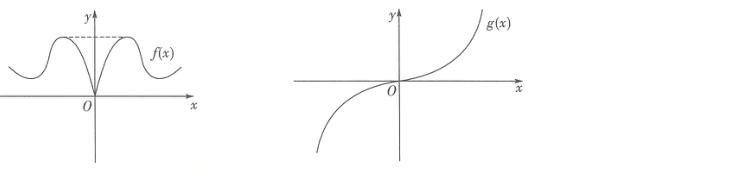
\includegraphics[width=.84\linewidth,height=.38\textheight,keepaspectratio]{figures/C03-HW085-5-source.png}\end{center}
{\footnotesize 补图来源：所给答案册PDF第24页（册内23页），已核对对应关系。}\par
{\small \field{关联知识}{F08 奇偶性、对称与函数性质应用（教材帮p.113、114、115 / PDF122、123、124）；F04 函数三种表示法、图象与读数（教材帮p.85、86、93、94 / PDF94、95、102、103）}
\field{方法与易错点}{检查定义域，再代入 $-x$；求另一侧解析式时同时写出 $-x$ 所在区间。 易错：只看公式不看定义域；用一对点证明奇偶；负半轴代换遗漏最外层负号。}
\field{答案依据}{答案册相关题组：PDF第23、24页（册内页22、23）；按当前题库原题逐项重算，不按旧版题号机械对套。}}

\itemhead{习题3.2 · 第6题（教材p.86）}{XJ-B1-C03-HW-P086-Y0231}
\label{XJ-B1-C03-HW-P086-Y0231}
{\footnotesize 湘教版教材p.86 / PDF第93页 / 习题3.2 / 第6题}
\field{原题}{已知函数 $f(x)$ 为奇函数，当 $x>0$ 时，$f(x)=x^2+\dfrac1x$，求 $f(-1)$。}
\field{参考答案}{$f(-1)=-f(1)=-2$。}
{\small \field{关联知识}{F08 奇偶性、对称与函数性质应用（教材帮p.113、114、115 / PDF122、123、124）；F03 函数求值、解析式与函数建模（教材帮p.80、87、88、89、90、131 / PDF89、96、97、98、99、140）}
\field{方法与易错点}{检查定义域，再代入 $-x$；求另一侧解析式时同时写出 $-x$ 所在区间。 易错：只看公式不看定义域；用一对点证明奇偶；负半轴代换遗漏最外层负号。}
\field{答案依据}{答案册相关题组：PDF第23、24页（册内页22、23）；按当前题库原题逐项重算，不按旧版题号机械对套。}}

\itemhead{习题3.2 · 第7题（教材p.86）}{XJ-B1-C03-HW-P086-Y0288}
\label{XJ-B1-C03-HW-P086-Y0288}
{\footnotesize 湘教版教材p.86 / PDF第93页 / 习题3.2 / 第7题}
\field{原题}{已知函数 $f(x)$ 是定义在 $\mathbb R$ 上的偶函数，当 $x\ge0$ 时，$f(x)=2x(x+4)$，试求出函数 $f(x)$ 在 $\mathbb R$ 上的解析式。}
\field{参考答案}{$f(x)=2x^2+8|x|$，$x\in\mathbb R$；分段写为 $2x^2-8x$（$x<0$）、$2x^2+8x$（$x\ge0$）。}
{\small \field{关联知识}{F08 奇偶性、对称与函数性质应用（教材帮p.113、114、115 / PDF122、123、124）；F03 函数求值、解析式与函数建模（教材帮p.80、87、88、89、90、131 / PDF89、96、97、98、99、140）}
\field{方法与易错点}{检查定义域，再代入 $-x$；求另一侧解析式时同时写出 $-x$ 所在区间。 易错：只看公式不看定义域；用一对点证明奇偶；负半轴代换遗漏最外层负号。}
\field{答案依据}{答案册相关题组：PDF第23、24页（册内页22、23）；按当前题库原题逐项重算，不按旧版题号机械对套。}}

\itemhead{习题3.2 · 第8题（教材p.86）}{XJ-B1-C03-HW-P086-Y0520}
\label{XJ-B1-C03-HW-P086-Y0520}
{\footnotesize 湘教版教材p.86 / PDF第93页 / 习题3.2 / 第8题}
\field{原题}{设函数 $f(x)$ 的定义域为 $(-4,5)$，如果 $f(x)$ 在 $(-4,0)$ 上是减函数，在 $(0,5)$ 上也是减函数，能不能断定它在 $(-4,5)$ 上是减函数？如果 $f(x)$ 在 $(-4,0]$ 上是增函数，在 $[0,5)$ 上也是增函数，能不能断定它在 $(-4,5)$ 上是增函数？}
\field{参考答案}{第一问不能。例如 $f(x)=-x$（$x<0$）、$f(x)=100-x$（$x>0$），任取 $f(0)$，两侧递减但跨0不递减。第二问能：跨0时由 $f(x_1)<f(0)<f(x_2)$ 推出，且两段包含公共点0。}
{\small \field{关联知识}{F05 单调性定义、证明与参数（教材帮p.97、98、100 / PDF106、107、109）}
\field{方法与易错点}{用定义比较任意两值，或依据已知图象性质；含参时使指定区间被相应单调区间覆盖。 易错：用有限采样代替证明；把分离半轴合并；漏跨零点情形。}
\field{答案依据}{答案册相关题组：PDF第23、24页（册内页22、23）；按当前题库原题逐项重算，不按旧版题号机械对套。}}

\itemhead{习题3.2 · 第9题（教材p.86）}{XJ-B1-C03-HW-P086-Y0708}
\label{XJ-B1-C03-HW-P086-Y0708}
{\footnotesize 湘教版教材p.86 / PDF第93页 / 习题3.2 / 第9题}
\field{原题}{已知函数 $f(x)=\dfrac x{x-a}$。
\subq{1}若 $a=-2$，证明：$f(x)$ 在 $(-\infty,-2)$ 上单调递增；
\subq{2}若 $a>0$，且 $f(x)$ 在 $(1,+\infty)$ 上单调递减，求 $a$ 的取值范围。}
\field{参考答案}{（1）差 $f(x_2)-f(x_1)=2(x_2-x_1)/[(x_1+2)(x_2+2)]>0$；（2）$a\in(0,1]$。需区间内无极点，故 $a\le1$；差为 $-a(x_2-x_1)/[(x_1-a)(x_2-a)]<0$，充分性也成立。}
{\small \field{关联知识}{F05 单调性定义、证明与参数（教材帮p.97、98、100 / PDF106、107、109）；F02 定义域与原式限制（教材帮p.79、80、81 / PDF88、89、90）}
\field{方法与易错点}{用定义比较任意两值，或依据已知图象性质；含参时使指定区间被相应单调区间覆盖。 易错：用有限采样代替证明；把分离半轴合并；漏跨零点情形。}
\field{答案依据}{答案册相关题组：PDF第23、24页（册内页22、23）；按当前题库原题逐项重算，不按旧版题号机械对套。}}

\itemhead{习题3.2 · 第10题（教材p.86）}{XJ-B1-C03-HW-P086-Y0853}
\label{XJ-B1-C03-HW-P086-Y0853}
{\footnotesize 湘教版教材p.86 / PDF第93页 / 习题3.2 / 第10题}
\field{原题}{下列函数中，既是奇函数又是增函数的有哪些？
\subq{1}$y=x+1$；
\subq{2}$y=\dfrac1x$；
\subq{3}$y=-x-\dfrac1x$；
\subq{4}$y=x|x|$。}
\field{参考答案}{只有（4）$y=x|x|$。两侧分别为 $-x^2,x^2$，各递增且跨0也递增；（2）在两半轴各递减，（3）不全域递增。}
{\small \field{关联知识}{F08 奇偶性、对称与函数性质应用（教材帮p.113、114、115 / PDF122、123、124）；F05 单调性定义、证明与参数（教材帮p.97、98、100 / PDF106、107、109）}
\field{方法与易错点}{检查定义域，再代入 $-x$；求另一侧解析式时同时写出 $-x$ 所在区间。 易错：只看公式不看定义域；用一对点证明奇偶；负半轴代换遗漏最外层负号。}
\field{答案依据}{答案册相关题组：PDF第23、24页（册内页22、23）；按当前题库原题逐项重算，不按旧版题号机械对套。}}

\itemhead{习题3.2 · 第11题（教材p.86）}{XJ-B1-C03-HW-P086-Y1034}
\label{XJ-B1-C03-HW-P086-Y1034}
{\footnotesize 湘教版教材p.86 / PDF第93页 / 习题3.2 / 第11题}
\field{原题}{设偶函数 $f(x)$ 的定义域为 $\mathbb R$，当 $x\in[0,+\infty)$ 时，$f(x)$ 是减函数，试确定 $f(-2),f(\pi),f(-3)$ 之间的大小关系。}
\field{参考答案}{$f(-2)>f(-3)>f(\pi)$，由偶性化为正半轴比较 $2<3<\pi$。}
{\small \field{关联知识}{F08 奇偶性、对称与函数性质应用（教材帮p.113、114、115 / PDF122、123、124）；F05 单调性定义、证明与参数（教材帮p.97、98、100 / PDF106、107、109）}
\field{方法与易错点}{检查定义域，再代入 $-x$；求另一侧解析式时同时写出 $-x$ 所在区间。 易错：只看公式不看定义域；用一对点证明奇偶；负半轴代换遗漏最外层负号。}
\field{答案依据}{答案册相关题组：PDF第23、24页（册内页22、23）；按当前题库原题逐项重算，不按旧版题号机械对套。}}

\itemhead{习题3.2 · 第12题（教材p.86）}{XJ-B1-C03-HW-P086-Y1121}
\label{XJ-B1-C03-HW-P086-Y1121}
{\footnotesize 湘教版教材p.86 / PDF第93页 / 习题3.2 / 第12题}
\field{原题}{已知 $f(x),g(x)$ 分别是定义在 $\mathbb R$ 上的偶函数和奇函数，且 $f(x)-g(x)=x^3+x^2+1$，求 $f(1)+g(1)$。}
\field{参考答案}{将 $x$ 换成 $-x$ 后相加相减得 $f(x)=x^2+1,g(x)=-x^3$，故 $f(1)+g(1)=1$。}
{\small \field{关联知识}{F08 奇偶性、对称与函数性质应用（教材帮p.113、114、115 / PDF122、123、124）；F03 函数求值、解析式与函数建模（教材帮p.80、87、88、89、90、131 / PDF89、96、97、98、99、140）}
\field{方法与易错点}{检查定义域，再代入 $-x$；求另一侧解析式时同时写出 $-x$ 所在区间。 易错：只看公式不看定义域；用一对点证明奇偶；负半轴代换遗漏最外层负号。}
\field{答案依据}{答案册相关题组：PDF第23、24页（册内页22、23）；按当前题库原题逐项重算，不按旧版题号机械对套。}}

\itemhead{习题3.2 · 第13题（教材p.86）}{XJ-B1-C03-HW-P086-Y1208}
\label{XJ-B1-C03-HW-P086-Y1208}
{\footnotesize 湘教版教材p.86 / PDF第93页 / 习题3.2 / 第13题}
\field{原题}{设函数 $f(x)$ 的定义域为 $\mathbb R$，且 $f(1+x)=f(1-x)$。若当 $x\ge1$ 时，$f(x)=x^2-1$，试确定 $f\left(\dfrac13\right),f\left(\dfrac23\right),f\left(\dfrac32\right)$ 之间的大小关系。}
\field{参考答案}{$f(2/3)=7/9<f(3/2)=5/4<f(1/3)=16/9$。关于 $x=1$ 对称，分别将 $1/3,2/3$ 映到 $5/3,4/3$。}
{\small \field{关联知识}{F08 奇偶性、对称与函数性质应用（教材帮p.113、114、115 / PDF122、123、124）；F05 单调性定义、证明与参数（教材帮p.97、98、100 / PDF106、107、109）}
\field{方法与易错点}{检查定义域，再代入 $-x$；求另一侧解析式时同时写出 $-x$ 所在区间。 易错：只看公式不看定义域；用一对点证明奇偶；负半轴代换遗漏最外层负号。}
\field{答案依据}{答案册相关题组：PDF第23、24页（册内页22、23）；按当前题库原题逐项重算，不按旧版题号机械对套。}}

\itemhead{第3章 小结与复习 · 第1题（教材p.89）}{XJ-B1-C03-SU-P089-Y0854}
\label{XJ-B1-C03-SU-P089-Y0854}
{\footnotesize 湘教版教材p.89 / PDF第96页 / 第3章 小结与复习 / 第1题}
\field{原题}{初中已学习函数的概念，在本章，我们进一步用更加严谨的集合和对应语言来刻画函数，突出了函数概念的本质是一个数集到另一个数集的一种确定的对应关系，明确了构成函数的要素，并引入函数符号 $y=f(x)$。通过本章的学习，你对函数概念有什么新的认识和体会吗？}
\field{参考答案}{函数是非空数集之间“每个输入都有且只有一个输出”的对应；相同函数看定义域与对应关系，值域由它们共同决定；不要求存在统一解析式，也不要求不同输入有不同输出。}
{\small \field{关联知识}{F01 函数本质、构成要素与相同函数（教材帮p.77、78 / PDF86、87）}
\field{方法与易错点}{逐一核对每个允许输入是否有且仅有一个合乎目标集合的输出。 易错：把值域直接当作目标集合；只看解析式外观；认为常函数不是函数。}
\field{答案依据}{答案册未提供本栏目的独立对应答案；依据原题、教材概念补写参考回应。开放性总结不设唯一数值答案。}}

\itemhead{第3章 小结与复习 · 第2题（教材p.89）}{XJ-B1-C03-SU-P089-Y1026}
\label{XJ-B1-C03-SU-P089-Y1026}
{\footnotesize 湘教版教材p.89 / PDF第96页 / 第3章 小结与复习 / 第2题}
\field{原题}{数学讲究表示。函数有哪几种常用的表示法？试结合具体实例，分析、比较这几种表示法的特点。}
\field{参考答案}{解析法便于精确求值和代数推理；列表法明确离散数据及对应；图象法直观显示变化和最值。三者应互相校验，图象读数通常受作图精度限制。}
{\small \field{关联知识}{F04 函数三种表示法、图象与读数（教材帮p.85、86、93、94 / PDF94、95、102、103）；F03 函数求值、解析式与函数建模（教材帮p.80、87、88、89、90、131 / PDF89、96、97、98、99、140）}
\field{方法与易错点}{把关键点与定义域一起标到图上，逐区间读交点和上下关系。 易错：将示意图预测当事实；把两曲线交点收进严格不等式；折线漏端点。}
\field{答案依据}{答案册未提供本栏目的独立对应答案；依据原题、教材概念补写参考回应。开放性总结不设唯一数值答案。}}

\itemhead{第3章 小结与复习 · 第3题（教材p.89）}{XJ-B1-C03-SU-P089-Y1112}
\label{XJ-B1-C03-SU-P089-Y1112}
{\footnotesize 湘教版教材p.89 / PDF第96页 / 第3章 小结与复习 / 第3题}
\field{原题}{根据函数的解析式或图象来探索它的性质，是数学的重要课题。函数的变化无非是变大变小，函数的单调性描述了函数的变化过程和趋势，是函数最重要的特征。如何判断一个函数的单调性？更进一步，你能用数学语言来表述吗？函数最值的几何意义如何理解？}
\field{参考答案}{单调性用区间内任意 $x_1<x_2$ 的函数值次序定义；最值 $M$ 要同时满足所有函数值不超过 $M$，并有某点实际取到 $M$。几何上为图象实际达到的最高或最低纵坐标。}
{\small \field{关联知识}{F05 单调性定义、证明与参数（教材帮p.97、98、100 / PDF106、107、109）；F06 最大值、最小值与值域（教材帮p.99、83、84 / PDF108、92、93）}
\field{方法与易错点}{用定义比较任意两值，或依据已知图象性质；含参时使指定区间被相应单调区间覆盖。 易错：用有限采样代替证明；把分离半轴合并；漏跨零点情形。}
\field{答案依据}{答案册未提供本栏目的独立对应答案；依据原题、教材概念补写参考回应。开放性总结不设唯一数值答案。}}

\itemhead{第3章 小结与复习 · 第4题（教材p.89）}{XJ-B1-C03-SU-P089-Y1284}
\label{XJ-B1-C03-SU-P089-Y1284}
{\footnotesize 湘教版教材p.89 / PDF第96页 / 第3章 小结与复习 / 第4题}
\field{原题}{如何判断一个函数的奇偶性？你能解释奇函数、偶函数图象的对称性吗？你能用数学语言来表述函数的奇偶性吗？}
\field{参考答案}{先查定义域对称性，再化简 $f(-x)$ 与 $f(x)$ 比较；偶函数图象关于 $y$ 轴对称，奇函数图象关于原点对称。只核对一对点不能证明恒等关系。}
{\small \field{关联知识}{F08 奇偶性、对称与函数性质应用（教材帮p.113、114、115 / PDF122、123、124）}
\field{方法与易错点}{检查定义域，再代入 $-x$；求另一侧解析式时同时写出 $-x$ 所在区间。 易错：只看公式不看定义域；用一对点证明奇偶；负半轴代换遗漏最外层负号。}
\field{答案依据}{答案册未提供本栏目的独立对应答案；依据原题、教材概念补写参考回应。开放性总结不设唯一数值答案。}}

\itemhead{第3章 小结与复习 · 第5题（教材p.89）}{XJ-B1-C03-SU-P089-Y1370}
\label{XJ-B1-C03-SU-P089-Y1370}
{\footnotesize 湘教版教材p.89 / PDF第96页 / 第3章 小结与复习 / 第5题}
\field{原题}{函数是描述客观世界变化规律的数学模型。函数的思想方法不仅将贯穿高中数学课程的始终，还会成为你今后学习或用到的数学知识的主旋律。小学到初中所学的数学知识，大都可以放到函数的框架之中；大量的实际问题，可以用函数模型来描述和解决。用函数的观点看数学和其他学科里的许多问题，常有纲举目张的效果。}
\field{参考答案}{示例：匀速运动 $s=vt$、购物 $y=px$、圆面积 $S=\pi r^2$ 均为函数模型。建模时明确自变量、实际定义域、单位、关系式，再用结果解释实际问题。本条为反思性总结，不设唯一数值答案。}
{\small \field{关联知识}{F03 函数求值、解析式与函数建模（教材帮p.80、87、88、89、90、131 / PDF89、96、97、98、99、140）}
\field{方法与易错点}{标清每次输入和输出；按已知函数类型或代换关系建立等价方程。 易错：将 $f(x)$ 当成 $f	imes x$；复合顺序反；换元后沿用错误定义域。}
\field{答案依据}{答案册未提供本栏目的独立对应答案；依据原题、教材概念补写参考回应。开放性总结不设唯一数值答案。}}

\itemhead{复习题三 · 第1题（教材p.90）}{XJ-B1-C03-RV-P090-Y0407}
\label{XJ-B1-C03-RV-P090-Y0407}
{\footnotesize 湘教版教材p.90 / PDF第97页 / 复习题三 / 第1题}
\field{原题}{判断下列对应是否为集合 $A$ 到集合 $B$ 的函数：
\subq{1}$A=\mathbb R$，$B=\{x\mid x>0\}$，$f:x\mapsto y=|x|$；
\subq{2}$A=\mathbb Z$，$B=\mathbb Z$，$f:x\mapsto y=x^2$；
\subq{3}$A=\mathbb Z$，$B=\mathbb Z$，$f:x\mapsto y=\sqrt x$；
\subq{4}$A=\{x\mid-1\le x\le1\}$，$B=\{0\}$，$f:x\mapsto y=0$。}
\field{参考答案}{依次为否、是、否、是。（1）$x=0$ 的值不在 $B$ 中；（3）负整数无实数平方根，部分正整数的平方根也不是整数。}
{\small \field{关联知识}{F01 函数本质、构成要素与相同函数（教材帮p.77、78 / PDF86、87）}
\field{方法与易错点}{逐一核对每个允许输入是否有且仅有一个合乎目标集合的输出。 易错：把值域直接当作目标集合；只看解析式外观；认为常函数不是函数。}
\field{答案依据}{答案册相关题组：PDF第24、25、26、27页（册内页23、24、25、26）；按当前题库原题逐项重算，不按旧版题号机械对套。}}

\itemhead{复习题三 · 第2题（教材p.90）}{XJ-B1-C03-RV-P090-Y0635}
\label{XJ-B1-C03-RV-P090-Y0635}
{\footnotesize 湘教版教材p.90 / PDF第97页 / 复习题三 / 第2题}
\field{原题}{求函数 $y=\sqrt{2x^2-x-2}$ 的定义域。}
\field{参考答案}{$(-\infty,(1-\sqrt{17})/4]\cup[(1+\sqrt{17})/4,+\infty)$。}
{\small \field{关联知识}{F02 定义域与原式限制（教材帮p.79、80、81 / PDF88、89、90）；I04 一元二次不等式与参数分类（教材帮p.64、65、66 / PDF73、74、75）}
\field{方法与易错点}{按原式逐项列条件后求交集，不先约分再判断。 易错：遗漏分母禁点；将函数值范围错当自变量范围；把退化矩形算入实际定义域。}
\field{答案依据}{答案册相关题组：PDF第24、25、26、27页（册内页23、24、25、26）；按当前题库原题逐项重算，不按旧版题号机械对套。}}

\itemhead{复习题三 · 第3题（教材p.90）}{XJ-B1-C03-RV-P090-Y0678}
\label{XJ-B1-C03-RV-P090-Y0678}
{\footnotesize 湘教版教材p.90 / PDF第97页 / 复习题三 / 第3题}
\field{原题}{已知 $f(x+1)=x^2+4x+1$，求函数 $f(x)$ 的解析式。}
\field{参考答案}{$f(x)=(x-1)^2+4(x-1)+1=x^2+2x-2$。}
{\small \field{关联知识}{F03 函数求值、解析式与函数建模（教材帮p.80、87、88、89、90、131 / PDF89、96、97、98、99、140）}
\field{方法与易错点}{标清每次输入和输出；按已知函数类型或代换关系建立等价方程。 易错：将 $f(x)$ 当成 $f	imes x$；复合顺序反；换元后沿用错误定义域。}
\field{答案依据}{答案册相关题组：PDF第24、25、26、27页（册内页23、24、25、26）；按当前题库原题逐项重算，不按旧版题号机械对套。}}

\itemhead{复习题三 · 第4题（教材p.90）}{XJ-B1-C03-RV-P090-Y0720}
\label{XJ-B1-C03-RV-P090-Y0720}
{\footnotesize 湘教版教材p.90 / PDF第97页 / 复习题三 / 第4题}
\field{原题}{已知函数 $y=f(x)$ 的对应关系如下表，函数 $y=g(x)$ 的图象是如图所示的曲线 $ABC$，其中 $A(1,3),B(2,1),C(3,2)$，则 $f(g(2))$ 的值为\blank。
\begin{center}\begin{tabular}{c|rrr}\hline$x$&1&2&3\\$f(x)$&2&3&0\\\hline\end{tabular}\end{center}
\bankfig{C03-RV090}{0.38}}
\field{参考答案}{$g(2)=1,f(1)=2$，故答案为2。}
{\small \field{关联知识}{F03 函数求值、解析式与函数建模（教材帮p.80、87、88、89、90、131 / PDF89、96、97、98、99、140）；F04 函数三种表示法、图象与读数（教材帮p.85、86、93、94 / PDF94、95、102、103）}
\field{方法与易错点}{标清每次输入和输出；按已知函数类型或代换关系建立等价方程。 易错：将 $f(x)$ 当成 $f	imes x$；复合顺序反；换元后沿用错误定义域。}
\field{答案依据}{答案册相关题组：PDF第24、25、26、27页（册内页23、24、25、26）；按当前题库原题逐项重算，不按旧版题号机械对套。}}

\itemhead{复习题三 · 第5题（教材p.90）}{XJ-B1-C03-RV-P090-Y1103}
\label{XJ-B1-C03-RV-P090-Y1103}
{\footnotesize 湘教版教材p.90 / PDF第97页 / 复习题三 / 第5题}
\field{原题}{已知函数 $f(x)=\begin{cases}2^x,&x>0,\\x+1,&x\le0,\end{cases}$ 若 $f(a)+f(1)=0$，求实数 $a$ 的值。}
\field{参考答案}{$f(1)=2$，故 $f(a)=-2$。$a>0$ 分支不可能为负；$a\le0$ 分支给 $a+1=-2$，得 $a=-3$。}
{\small \field{关联知识}{F07 分段函数、绝对值及分段应用（教材帮p.86、91、92、93 / PDF95、100、101、102）；F03 函数求值、解析式与函数建模（教材帮p.80、87、88、89、90、131 / PDF89、96、97、98、99、140）}
\field{方法与易错点}{先列转折点和各段条件，再建立分段式，检查衔接、定义域与值域。 易错：跨段套公式；超额部分按全量收费；绝对值去号漏区间。}
\field{答案依据}{答案册相关题组：PDF第24、25、26、27页（册内页23、24、25、26）；按当前题库原题逐项重算，不按旧版题号机械对套。}}

\itemhead{复习题三 · 第6题（教材p.90）}{XJ-B1-C03-RV-P090-Y1174}
\label{XJ-B1-C03-RV-P090-Y1174}
{\footnotesize 湘教版教材p.90 / PDF第97页 / 复习题三 / 第6题}
\field{原题}{已知函数 $f(x)=\sqrt{x^2-1}$，试判断 $f(x)$ 在区间 $[1,+\infty)$ 上的单调性，并加以证明。}
\field{参考答案}{递增。若 $1\le x_1<x_2$，则 $x_1^2-1<x_2^2-1$；平方根在非负数上保序，得 $f(x_1)<f(x_2)$。}
{\small \field{关联知识}{F05 单调性定义、证明与参数（教材帮p.97、98、100 / PDF106、107、109）}
\field{方法与易错点}{用定义比较任意两值，或依据已知图象性质；含参时使指定区间被相应单调区间覆盖。 易错：用有限采样代替证明；把分离半轴合并；漏跨零点情形。}
\field{答案依据}{答案册相关题组：PDF第24、25、26、27页（册内页23、24、25、26）；按当前题库原题逐项重算，不按旧版题号机械对套。}}

\itemhead{复习题三 · 第7题（教材p.90）}{XJ-B1-C03-RV-P090-Y1256}
\label{XJ-B1-C03-RV-P090-Y1256}
{\footnotesize 湘教版教材p.90 / PDF第97页 / 复习题三 / 第7题}
\field{原题}{求函数 $y=-x^2+4x-2$ 在区间 $[0,3]$ 上的最大值和最小值。}
\field{参考答案}{最大值2在 $x=2$ 取得；最小值 $-2$ 在 $x=0$ 取得。用配方 $-(x-2)^2+2$ 并比较两端点。}
{\small \field{关联知识}{F06 最大值、最小值与值域（教材帮p.99、83、84 / PDF108、92、93）；Q01 二次函数、零点、判别式与根系关系（教材帮p.65 / PDF74）}
\field{方法与易错点}{根据图象、配方、单调性或基本不等式找界，再验证取值点。 易错：把上界下界当最值；只比较两端漏顶点；只有最值却未说明全部值均可取。}
\field{答案依据}{答案册相关题组：PDF第24、25、26、27页（册内页23、24、25、26）；按当前题库原题逐项重算，不按旧版题号机械对套。}}

\itemhead{复习题三 · 第8题（教材p.90）}{XJ-B1-C03-RV-P090-Y1299}
\label{XJ-B1-C03-RV-P090-Y1299}
{\footnotesize 湘教版教材p.90 / PDF第97页 / 复习题三 / 第8题}
\field{原题}{已知二次函数 $f(x)$ 的图象关于 $y$ 轴对称，且在区间 $[0,+\infty)$ 上为增函数，试确定 $f(0),f(3),f(-4)$ 之间的大小关系。}
\field{参考答案}{$f(0)<f(3)<f(-4)$。先用偶性得 $f(-4)=f(4)$，再比较 $0<3<4$。}
{\small \field{关联知识}{F08 奇偶性、对称与函数性质应用（教材帮p.113、114、115 / PDF122、123、124）；F05 单调性定义、证明与参数（教材帮p.97、98、100 / PDF106、107、109）}
\field{方法与易错点}{检查定义域，再代入 $-x$；求另一侧解析式时同时写出 $-x$ 所在区间。 易错：只看公式不看定义域；用一对点证明奇偶；负半轴代换遗漏最外层负号。}
\field{答案依据}{答案册相关题组：PDF第24、25、26、27页（册内页23、24、25、26）；按当前题库原题逐项重算，不按旧版题号机械对套。}}

\itemhead{复习题三 · 第9题（教材p.90）}{XJ-B1-C03-RV-P090-Y1401}
\label{XJ-B1-C03-RV-P090-Y1401}
{\footnotesize 湘教版教材p.90 / PDF第97页 / 复习题三 / 第9题}
\field{原题}{已知函数 $f(x)=\dfrac{ax^2+1}{bx+c}\ (a,b,c\in\mathbb Z)$ 是奇函数，且 $f(1)=2,f(2)<3$，求 $a,b,c$ 的值。}
\field{参考答案}{$a=1,b=1,c=0$。奇函数的对称定义域与非零函数排除 $b=0$ 及非零极点的非对称情形，故 $c=0,b\ne0$；再由 $a+1=2b$、$(4a+1)/(2b)<3$ 和整数限制得唯一解。}
{\small \field{关联知识}{F08 奇偶性、对称与函数性质应用（教材帮p.113、114、115 / PDF122、123、124）；F02 定义域与原式限制（教材帮p.79、80、81 / PDF88、89、90）}
\field{方法与易错点}{检查定义域，再代入 $-x$；求另一侧解析式时同时写出 $-x$ 所在区间。 易错：只看公式不看定义域；用一对点证明奇偶；负半轴代换遗漏最外层负号。}
\field{答案依据}{答案册相关题组：PDF第24、25、26、27页（册内页23、24、25、26）；按当前题库原题逐项重算，不按旧版题号机械对套。}}

\itemhead{复习题三 · 第10题（教材p.90）}{XJ-B1-C03-RV-P090-Y1501}
\label{XJ-B1-C03-RV-P090-Y1501}
{\footnotesize 湘教版教材p.90 / PDF第97页 / 复习题三 / 第10题}
\field{原题}{已知函数 $f(x)=(x+1)(x+a)$ 为偶函数，求 $a$ 的值。}
\field{参考答案}{$a=-1$。展开后一次项系数 $a+1$ 必为0；此时函数为 $x^2-1$。}
{\small \field{关联知识}{F08 奇偶性、对称与函数性质应用（教材帮p.113、114、115 / PDF122、123、124）}
\field{方法与易错点}{检查定义域，再代入 $-x$；求另一侧解析式时同时写出 $-x$ 所在区间。 易错：只看公式不看定义域；用一对点证明奇偶；负半轴代换遗漏最外层负号。}
\field{答案依据}{答案册相关题组：PDF第24、25、26、27页（册内页23、24、25、26）；按当前题库原题逐项重算，不按旧版题号机械对套。}}

\itemhead{复习题三 · 第11题（教材p.90）}{XJ-B1-C03-RV-P090-Y1543}
\label{XJ-B1-C03-RV-P090-Y1543}
{\footnotesize 湘教版教材p.90 / PDF第97页 / 复习题三 / 第11题}
\field{原题}{某企业生产一种精密电子仪器的固定成本为 20000 元，每生产一台仪器需增加投入 100 元，已知总收益满足函数：
\[R(x)=\begin{cases}400x-\dfrac12x^2,&0\le x\le400,\\80000,&x>400,\end{cases}\]
其中 $x$ 是仪器的月产量。
\subq{1}将利润表示为月产量的函数。
\subq{2}当月产量为何值时，企业所获利润最大？最大利润是多少元？}
\field{参考答案}{（1）$L(x)=\begin{cases}-x^2/2+300x-20000,&0\le x\le400,\\60000-100x,&x>400.\end{cases}$，实际月产量取非负整数。（2）第一段配方为 $-(x-300)^2/2+25000$；第二段小于20000。故300台时最大利润25000元。}
{\small \field{关联知识}{F07 分段函数、绝对值及分段应用（教材帮p.86、91、92、93 / PDF95、100、101、102）；F06 最大值、最小值与值域（教材帮p.99、83、84 / PDF108、92、93）}
\field{方法与易错点}{先列转折点和各段条件，再建立分段式，检查衔接、定义域与值域。 易错：跨段套公式；超额部分按全量收费；绝对值去号漏区间。}
\field{答案依据}{答案册相关题组：PDF第24、25、26、27页（册内页23、24、25、26）；按当前题库原题逐项重算，不按旧版题号机械对套。}}

\itemhead{复习题三 · 第12题（教材p.91）}{XJ-B1-C03-RV-P091-Y0650}
\label{XJ-B1-C03-RV-P091-Y0650}
{\footnotesize 湘教版教材p.91 / PDF第98页 / 复习题三 / 第12题}
\field{原题}{（多选题）已知函数 $f(x)$ 满足 $f(x+y)=f(x)+f(y)\ (x,y\in\mathbb R)$，则（\quad）
\choice{A}$f(0)=0$
\choice{B}$f(x)$ 是奇函数
\choice{C}$f(x)$ 是偶函数
\choice{D}当 $f(2)=\sqrt5$ 时，$f(200)=100\sqrt5$}
\field{参考答案}{ABD。令 $x=y=0$ 得 $f(0)=0$；令 $y=-x$ 得奇性；$f(200)=100f(2)=100\sqrt5$。C不必成立，$f(x)=x$ 为反例。}
\field{核对说明}{多选设问变化：现教材需写ABD，答案册PDF25按三个证明小问给解，须转换为逐项判断。}
{\small \field{关联知识}{F08 奇偶性、对称与函数性质应用（教材帮p.113、114、115 / PDF122、123、124）；F03 函数求值、解析式与函数建模（教材帮p.80、87、88、89、90、131 / PDF89、96、97、98、99、140）}
\field{方法与易错点}{检查定义域，再代入 $-x$；求另一侧解析式时同时写出 $-x$ 所在区间。 易错：只看公式不看定义域；用一对点证明奇偶；负半轴代换遗漏最外层负号。}
\field{答案依据}{答案册相关题组：PDF第24、25、26、27页（册内页23、24、25、26）；按当前题库原题逐项重算，不按旧版题号机械对套。}}

\itemhead{复习题三 · 第13题（教材p.91）}{XJ-B1-C03-RV-P091-Y0785}
\label{XJ-B1-C03-RV-P091-Y0785}
{\footnotesize 湘教版教材p.91 / PDF第98页 / 复习题三 / 第13题}
\field{原题}{根据如图所示的图象，简要说明近 150 年来人类消耗的能源结构变化情况，并对未来 100 年能源结构的变化趋势作出预测。
\bankfig{C03-RV091}{0.7}}
\field{参考答案}{按所给历史示意图：木材比例总体下降，煤炭先升后降，石油先升后趋降，天然气和核能从出现后逐渐增加。未来趋势只能作基于此图的推测，可讨论核能、水合物和太阳能的份额增加；这不是现实能源统计或确定预测，不能用示意图编造实际数据。}
{\small \field{关联知识}{F04 函数三种表示法、图象与读数（教材帮p.85、86、93、94 / PDF94、95、102、103）}
\field{方法与易错点}{把关键点与定义域一起标到图上，逐区间读交点和上下关系。 易错：将示意图预测当事实；把两曲线交点收进严格不等式；折线漏端点。}
\field{答案依据}{答案册相关题组：PDF第24、25、26、27页（册内页23、24、25、26）；按当前题库原题逐项重算，不按旧版题号机械对套。}}

\itemhead{复习题三 · 第14题（教材p.91）}{XJ-B1-C03-RV-P091-Y1267}
\label{XJ-B1-C03-RV-P091-Y1267}
{\footnotesize 湘教版教材p.91 / PDF第98页 / 复习题三 / 第14题}
\field{原题}{某市对家庭每月用水的收费规定为：若用水量不超过基本月用水量 $a\,\mathrm{m^3}$，则只付基本费 8 元和损耗费 $c\ (c<5)$ 元；若用水量超过基本月用水量，则除了需付基本费和损耗费外，超过部分还需按 $b$ 元/$\mathrm{m^3}$ 进行付费。已知该市某家庭 1—3 月的用水量分别为 $9\,\mathrm{m^3},15\,\mathrm{m^3}$ 和 $22\,\mathrm{m^3}$，其支付的费用分别为 9 元、19 元和 33 元。试写出每月支付费用 $y$（元）关于月用水量 $x$（$\mathrm{m^3}$）的函数，并画出函数的图象。}
\field{参考答案}{$a=10,b=2,c=1$，故 $y=9$（$0\le x\le10$）、$y=2x-11$（$x>10$）。图象为水平线段与从 $(10,9)$ 向右上延伸的射线，两段在边界衔接。}
\begin{center}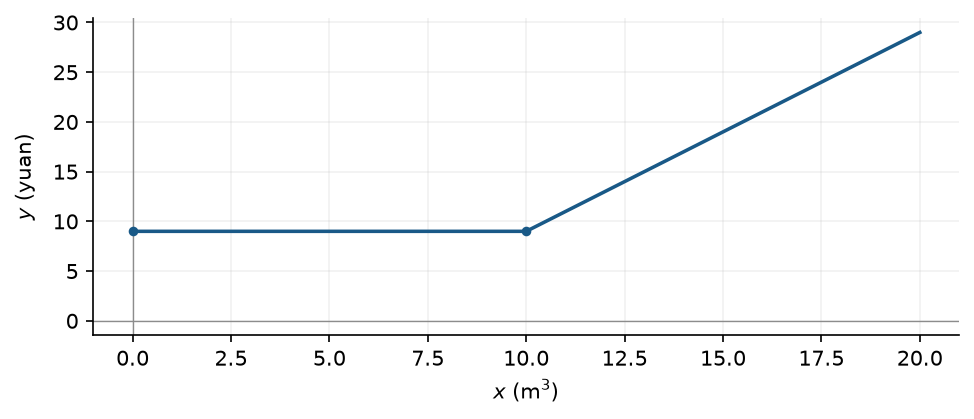
\includegraphics[width=.84\linewidth,height=.38\textheight,keepaspectratio]{figures/C03-RV091-14.png}\end{center}
{\small \field{关联知识}{F07 分段函数、绝对值及分段应用（教材帮p.86、91、92、93 / PDF95、100、101、102）；F03 函数求值、解析式与函数建模（教材帮p.80、87、88、89、90、131 / PDF89、96、97、98、99、140）}
\field{方法与易错点}{先列转折点和各段条件，再建立分段式，检查衔接、定义域与值域。 易错：跨段套公式；超额部分按全量收费；绝对值去号漏区间。}
\field{答案依据}{答案册相关题组：PDF第24、25、26、27页（册内页23、24、25、26）；按当前题库原题逐项重算，不按旧版题号机械对套。}}

\itemhead{复习题三 · 第15题（教材p.91）}{XJ-B1-C03-RV-P091-Y1481}
\label{XJ-B1-C03-RV-P091-Y1481}
{\footnotesize 湘教版教材p.91 / PDF第98页 / 复习题三 / 第15题}
\field{原题}{已知某函数在区间 $(-\infty,1]$ 上单调递减，在区间 $[1,+\infty)$ 上单调递增，且 $f(1)=1$。试写出一个这样的函数解析式。}
\field{参考答案}{例如 $f(x)=(x-1)^2+1$，或 $f(x)=|x-1|+1$，均满足；答案不唯一。}
\begin{center}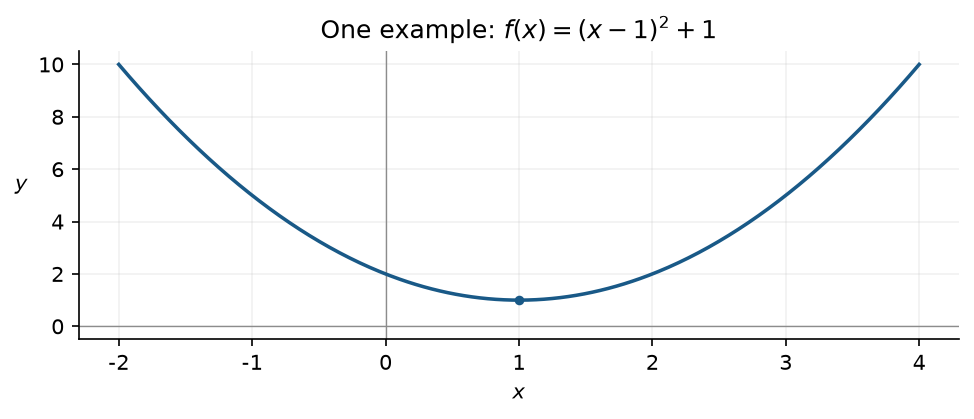
\includegraphics[width=.84\linewidth,height=.38\textheight,keepaspectratio]{figures/C03-RV091-15.png}\end{center}
{\small \field{关联知识}{F05 单调性定义、证明与参数（教材帮p.97、98、100 / PDF106、107、109）；F06 最大值、最小值与值域（教材帮p.99、83、84 / PDF108、92、93）}
\field{方法与易错点}{用定义比较任意两值，或依据已知图象性质；含参时使指定区间被相应单调区间覆盖。 易错：用有限采样代替证明；把分离半轴合并；漏跨零点情形。}
\field{答案依据}{答案册相关题组：PDF第24、25、26、27页（册内页23、24、25、26）；按当前题库原题逐项重算，不按旧版题号机械对套。}}

\itemhead{复习题三 · 第16题（教材p.92）}{XJ-B1-C03-RV-P092-Y0231}
\label{XJ-B1-C03-RV-P092-Y0231}
{\footnotesize 湘教版教材p.92 / PDF第99页 / 复习题三 / 第16题}
\field{原题}{若函数 $f(x)=2x+\dfrac mx$ 在区间 $(0,2]$ 上是减函数，求实数 $m$ 的取值范围。}
\field{参考答案}{$m\ge8$。差 $f(x_2)-f(x_1)=(x_2-x_1)(2-m/(x_1x_2))$。$0<x_1<x_2\le2$ 时乘积小于4；$m\ge8$ 保证差严格负。若 $m<8$，在2附近取两点使乘积充分接近4则差为正，必要性成立。}
{\small \field{关联知识}{F05 单调性定义、证明与参数（教材帮p.97、98、100 / PDF106、107、109）；I06 恒成立、有解与范围内最值（教材帮p.71、72、73 / PDF80、81、82）}
\field{方法与易错点}{用定义比较任意两值，或依据已知图象性质；含参时使指定区间被相应单调区间覆盖。 易错：用有限采样代替证明；把分离半轴合并；漏跨零点情形。}
\field{答案依据}{答案册相关题组：PDF第24、25、26、27页（册内页23、24、25、26）；按当前题库原题逐项重算，不按旧版题号机械对套。}}

\itemhead{复习题三 · 第17题（教材p.92）}{XJ-B1-C03-RV-P092-Y0288}
\label{XJ-B1-C03-RV-P092-Y0288}
{\footnotesize 湘教版教材p.92 / PDF第99页 / 复习题三 / 第17题}
\field{原题}{若偶函数 $f(x)$ 在区间 $[-8,-5]$ 上单调递减且在区间 $[-5,-1]$ 上单调递增，试讨论 $f(x)$ 在区间 $[2,7]$ 上的单调性，并进一步讨论 $f(x)$ 为奇函数的情形。}
\field{参考答案}{偶函数情形：在 $[2,5]$ 递减、$[5,7]$ 递增；奇函数情形：在 $[2,5]$ 递增、$[5,7]$ 递减。偶函数两侧次序相反，奇函数对称两侧的单调方向相同。}
{\small \field{关联知识}{F08 奇偶性、对称与函数性质应用（教材帮p.113、114、115 / PDF122、123、124）；F05 单调性定义、证明与参数（教材帮p.97、98、100 / PDF106、107、109）}
\field{方法与易错点}{检查定义域，再代入 $-x$；求另一侧解析式时同时写出 $-x$ 所在区间。 易错：只看公式不看定义域；用一对点证明奇偶；负半轴代换遗漏最外层负号。}
\field{答案依据}{答案册相关题组：PDF第24、25、26、27页（册内页23、24、25、26）；按当前题库原题逐项重算，不按旧版题号机械对套。}}

\itemhead{复习题三 · 第18题（教材p.92）}{XJ-B1-C03-RV-P092-Y0375}
\label{XJ-B1-C03-RV-P092-Y0375}
{\footnotesize 湘教版教材p.92 / PDF第99页 / 复习题三 / 第18题}
\field{原题}{已知函数 $y=f(x)$ 与 $y=g(x)$ 的图象如图所示，则函数 $y=f(x)\cdot g(x)$ 的图象可能是（\quad）
\bankfig{C03-RV092}{0.88}}
\field{参考答案}{A。$f$ 偶、$g$ 奇，乘积为奇函数；在0右侧邻近处 $f>0,g<0$，乘积为负，排除其他图象。}
{\small \field{关联知识}{F04 函数三种表示法、图象与读数（教材帮p.85、86、93、94 / PDF94、95、102、103）；F08 奇偶性、对称与函数性质应用（教材帮p.113、114、115 / PDF122、123、124）}
\field{方法与易错点}{把关键点与定义域一起标到图上，逐区间读交点和上下关系。 易错：将示意图预测当事实；把两曲线交点收进严格不等式；折线漏端点。}
\field{答案依据}{答案册相关题组：PDF第24、25、26、27页（册内页23、24、25、26）；按当前题库原题逐项重算，不按旧版题号机械对套。}}

\itemhead{复习题三 · 第19题（教材p.92）}{XJ-B1-C03-RV-P092-Y1067}
\label{XJ-B1-C03-RV-P092-Y1067}
{\footnotesize 湘教版教材p.92 / PDF第99页 / 复习题三 / 第19题}
\field{原题}{探索并回答下列问题：
\subq{1}把 $y=\dfrac1x$ 的图象向右平移 1 个单位长度，求所得图象的函数解析式；
\subq{2}把 $y=\dfrac1x$ 的图象向左平移 2 个单位长度，求所得图象的函数解析式；
\subq{3}把 $y=\dfrac1x$ 的图象向上平移 1 个单位长度，求所得图象的函数解析式；
\subq{4}把 $y=\dfrac1x$ 的图象向下平移 2 个单位长度，求所得图象的函数解析式。
对于任意函数 $y=f(x)$，你能写出它的图象平移与解析式的变化规律吗？试一试。}
\field{参考答案}{依次为 $1/(x-1)$（$x\ne1$）、$1/(x+2)$（$x\ne-2$）、$1/x+1$、$1/x-2$（后二式 $x\ne0$）。一般向右平移 $h$ 用 $f(x-h)$，向上平移 $k$ 用 $f(x)+k$；定义域也随水平平移改变。}
\begin{center}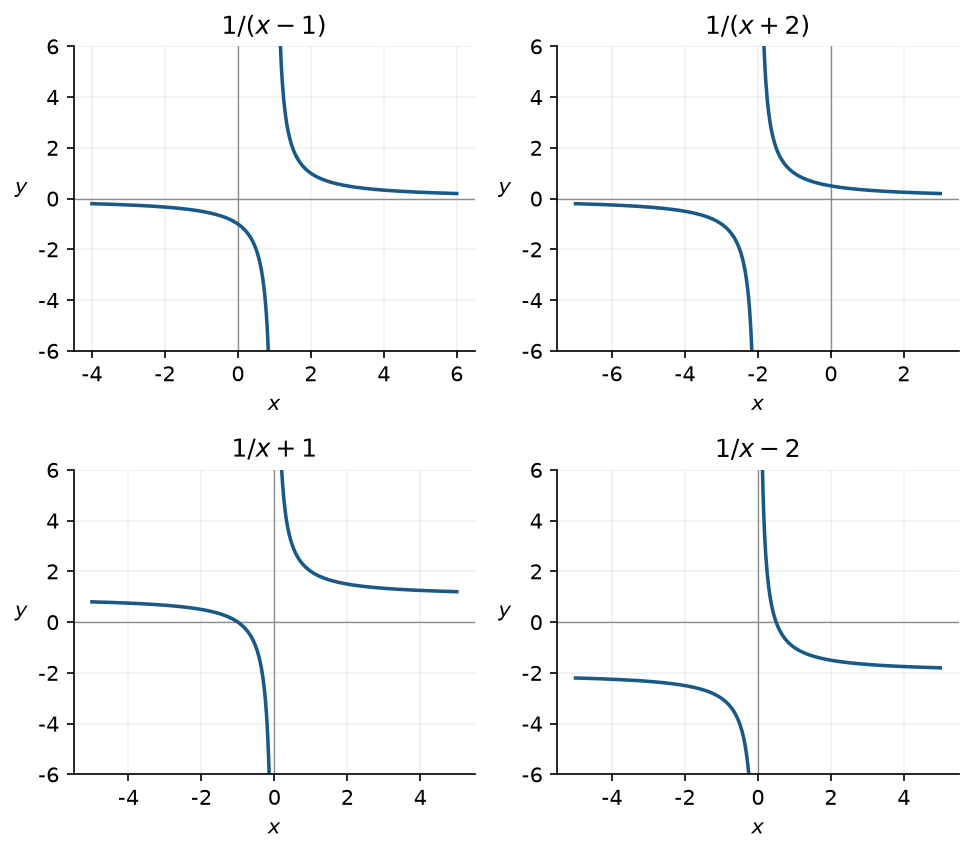
\includegraphics[width=.84\linewidth,height=.38\textheight,keepaspectratio]{figures/C03-RV092-19.png}\end{center}
{\small \field{关联知识}{F09 图象平移、伸缩与对称（教材帮p.86、94 / PDF95、103）；F02 定义域与原式限制（教材帮p.79、80、81 / PDF88、89、90）}
\field{方法与易错点}{追踪点 $(u,f(u))$ 变换后的坐标，反推新解析式。 易错：平移只改公式而未改定义域；把纵向倍率当作指数底数变化。}
\field{答案依据}{答案册相关题组：PDF第24、25、26、27页（册内页23、24、25、26）；按当前题库原题逐项重算，不按旧版题号机械对套。}}

\itemhead{复习题三 · 第20题（教材p.92）}{XJ-B1-C03-RV-P092-Y1491}
\label{XJ-B1-C03-RV-P092-Y1491}
{\footnotesize 湘教版教材p.92 / PDF第99页 / 复习题三 / 第20题}
\field{原题}{探索函数 $y=x+\dfrac cx$（常数 $c>0$）的奇偶性、值域以及单调性，并说明理由；若函数为 $y=x^2+\dfrac c{x^2}$（常数 $c>0$），该函数的性质有何变化？}
\field{参考答案}{第一函数定义域 $\mathbb R\setminus\{0\}$，为奇函数，值域 $(-\infty,-2\sqrt c]\cup[2\sqrt c,+\infty)$；增区间 $(-\infty,-\sqrt c],[\sqrt c,+\infty)$，减区间 $[-\sqrt c,0),(0,\sqrt c]$。差式为 $(x_2-x_1)(1-c/(x_1x_2))$。第二函数为偶函数，值域 $[2\sqrt c,+\infty)$；令 $r=\sqrt[4]c$，增区间 $[-r,0),[r,+\infty)$，减区间 $(-\infty,-r],(0,r]$；用 $t=x^2>0$ 及基本不等式证明。两个断开的区间须分别写，不合并成单调区间。}
{\small \field{关联知识}{F08 奇偶性、对称与函数性质应用（教材帮p.113、114、115 / PDF122、123、124）；F05 单调性定义、证明与参数（教材帮p.97、98、100 / PDF106、107、109）；F06 最大值、最小值与值域（教材帮p.99、83、84 / PDF108、92、93）}
\field{方法与易错点}{检查定义域，再代入 $-x$；求另一侧解析式时同时写出 $-x$ 所在区间。 易错：只看公式不看定义域；用一对点证明奇偶；负半轴代换遗漏最外层负号。}
\field{答案依据}{答案册相关题组：PDF第24、25、26、27页（册内页23、24、25、26）；按当前题库原题逐项重算，不按旧版题号机械对套。}}

\section{第4章 幂函数、指数函数和对数函数（至4.2）}
\itemhead{4.1 例题 · 例题1（教材p.95）}{XJ-B1-C04-EX-P095-Y0782}
\label{XJ-B1-C04-EX-P095-Y0782}
{\footnotesize 湘教版教材p.95 / PDF第102页 / 4.1 例题 / 例题1}
\field{原题}{化简下列各式：
\subq{1}$\sqrt[3]{(-2)^3}$；
\subq{2}$\sqrt[4]{(-2)^4}$；
\subq{3}$\sqrt[3]{(3-a)^3}$；
\subq{4}$\sqrt{(a-b)^2}\ (a<b)$；
\subq{5}$\sqrt{(3-a)^2}$。}
\field{参考答案}{依次为 $-2,2,3-a,b-a,|3-a|$。偶次根号所得值非负。}
{\small \field{关联知识}{P01 方根、根式与绝对值（教材帮p.143 / PDF152）}
\field{方法与易错点}{先看根指数奇偶，再检查被开方数符号，必要时写绝对值分段。 易错：把偶次根式值写成正负两个；$\sqrt{a^2}$ 直接写 $a$。}
\field{答案依据}{例题原解位置：湘教版教材p.95及题库原图；独立编写可编辑参考解答。答案册此部分主要收练习、习题，不伪造例题答案册位置。}}

\itemhead{4.1 例题 · 例题2（教材p.96）}{XJ-B1-C04-EX-P096-Y0533}
\label{XJ-B1-C04-EX-P096-Y0533}
{\footnotesize 湘教版教材p.96 / PDF第103页 / 4.1 例题 / 例题2}
\field{原题}{求下列各式的值：
\subq{1}$16^{3/4}$；
\subq{2}$25^{-1/2}$；
\subq{3}$\left(\dfrac13\right)^{-3}$；
\subq{4}$\left(\dfrac{125}{64}\right)^{-2/3}$。}
\field{参考答案}{依次为 $8,1/5,27,16/25$。}
{\small \field{关联知识}{P02 有理数、实数指数幂与运算（教材帮p.144、145 / PDF153、154）}
\field{方法与易错点}{统一为指数幂，分开处理系数与各底数的指数；最终复查定义条件及数值精度。 易错：负指数误作负数；幂的幂指数相加；约分丢禁点；过早四舍五入。}
\field{答案依据}{例题原解位置：湘教版教材p.96及题库原图；独立编写可编辑参考解答。答案册此部分主要收练习、习题，不伪造例题答案册位置。}}

\itemhead{4.1 例题 · 例题3（教材p.96）}{XJ-B1-C04-EX-P096-Y0978}
\label{XJ-B1-C04-EX-P096-Y0978}
{\footnotesize 湘教版教材p.96 / PDF第103页 / 4.1 例题 / 例题3}
\field{原题}{用分数指数幂的形式表示下列各式，其中 $a>0$：
\subq{1}$a\cdot\sqrt[3]a$；
\subq{2}$a^2\cdot\sqrt[4]{a^3}$；
\subq{3}$\sqrt{a\sqrt[3]a}$。}
\field{参考答案}{依次为 $a^{4/3},a^{11/4},a^{2/3}$，$a>0$。}
{\small \field{关联知识}{P02 有理数、实数指数幂与运算（教材帮p.144、145 / PDF153、154）}
\field{方法与易错点}{统一为指数幂，分开处理系数与各底数的指数；最终复查定义条件及数值精度。 易错：负指数误作负数；幂的幂指数相加；约分丢禁点；过早四舍五入。}
\field{答案依据}{例题原解位置：湘教版教材p.96及题库原图；独立编写可编辑参考解答。答案册此部分主要收练习、习题，不伪造例题答案册位置。}}

\itemhead{4.1 例题 · 例题4（教材p.96）}{XJ-B1-C04-EX-P096-Y1306}
\label{XJ-B1-C04-EX-P096-Y1306}
{\footnotesize 湘教版教材p.96 / PDF第103页 / 4.1 例题 / 例题4}
\field{原题}{计算下列各式（式中字母都表示正数）：
\subq{1}$\left(a^{1/3}b^{-5/6}\right)^6$；
\subq{2}$\left(3m^{3/4}n^{3/2}\right)\cdot\left(-4m^{-1/4}n^{1/3}\right)\div\left(-6m^{1/2}n^{5/6}\right)$。}
\field{参考答案}{（1）$a^2b^{-5}$；（2）$2n$。第二问 $m$ 的指数相加减为0，$n$ 的指数为1。}
{\small \field{关联知识}{P02 有理数、实数指数幂与运算（教材帮p.144、145 / PDF153、154）}
\field{方法与易错点}{统一为指数幂，分开处理系数与各底数的指数；最终复查定义条件及数值精度。 易错：负指数误作负数；幂的幂指数相加；约分丢禁点；过早四舍五入。}
\field{答案依据}{例题原解位置：湘教版教材p.96及题库原图；独立编写可编辑参考解答。答案册此部分主要收练习、习题，不伪造例题答案册位置。}}

\itemhead{4.1 例题 · 例题5（教材p.97）}{XJ-B1-C04-EX-P097-Y0403}
\label{XJ-B1-C04-EX-P097-Y0403}
{\footnotesize 湘教版教材p.97 / PDF第104页 / 4.1 例题 / 例题5}
\field{原题}{利用分数指数幂表示根式，化简下列各式（式中字母都表示正数）：
\subq{1}$\dfrac{\sqrt[3]{a^2}\cdot\sqrt b}{\sqrt a\cdot\sqrt[3]b}$；
\subq{2}$\left(\sqrt[3]a-\sqrt{a^3}\right)\div\sqrt[6]a$；
\subq{3}$\sqrt[3]{xy^2\left(\sqrt{xy}\right)^3}$。}
\field{参考答案}{依次为 $a^{1/6}b^{1/6}$；$a^{1/6}-a^{4/3}$；$x^{5/6}y^{7/6}$。}
{\small \field{关联知识}{P02 有理数、实数指数幂与运算（教材帮p.144、145 / PDF153、154）}
\field{方法与易错点}{统一为指数幂，分开处理系数与各底数的指数；最终复查定义条件及数值精度。 易错：负指数误作负数；幂的幂指数相加；约分丢禁点；过早四舍五入。}
\field{答案依据}{例题原解位置：湘教版教材p.97及题库原图；独立编写可编辑参考解答。答案册此部分主要收练习、习题，不伪造例题答案册位置。}}

\itemhead{p.97 练习 · 第1题（教材p.97）}{XJ-B1-C04-PR-P097-Y0891}
\label{XJ-B1-C04-PR-P097-Y0891}
{\footnotesize 湘教版教材p.97 / PDF第104页 / p.97 练习 / 第1题}
\field{原题}{用根式表示下列各式（$a>0$）：
\subq{1}$a^{1/3}$；
\subq{2}$a^{2/3}$；
\subq{3}$a^{-2/3}$；
\subq{4}$a^{-3/2}$。}
\field{参考答案}{依次为 $\sqrt[3]a,\sqrt[3]{a^2},1/\sqrt[3]{a^2},1/\sqrt{a^3}$。}
{\small \field{关联知识}{P02 有理数、实数指数幂与运算（教材帮p.144、145 / PDF153、154）}
\field{方法与易错点}{统一为指数幂，分开处理系数与各底数的指数；最终复查定义条件及数值精度。 易错：负指数误作负数；幂的幂指数相加；约分丢禁点；过早四舍五入。}
\field{答案依据}{答案册相关题组：PDF第30页（册内页29）；按当前题库原题逐项重算，不按旧版题号机械对套。}}

\itemhead{p.97 练习 · 第2题（教材p.97）}{XJ-B1-C04-PR-P097-Y1020}
\label{XJ-B1-C04-PR-P097-Y1020}
{\footnotesize 湘教版教材p.97 / PDF第104页 / p.97 练习 / 第2题}
\field{原题}{用分数指数幂表示下列各式（式中字母都表示正数）：
\subq{1}$\sqrt[4]{a^3}$；
\subq{2}$\sqrt[4]{(m+n)^3}$；
\subq{3}$\sqrt[5]{(a+2b)^2}$；
\subq{4}$\sqrt[4]{(m-n)^2}\ (m<n)$；
\subq{5}$\sqrt{a^4b^3}$；
\subq{6}$\dfrac{m^2}{\sqrt[3]m}$。}
\field{参考答案}{依次为 $a^{3/4},(m+n)^{3/4},(a+2b)^{2/5},(n-m)^{1/2},a^2b^{3/2},m^{5/3}$；第（4）利用 $m<n$，不能直接写负底数的 $1/2$ 次幂。}
{\small \field{关联知识}{P02 有理数、实数指数幂与运算（教材帮p.144、145 / PDF153、154）}
\field{方法与易错点}{统一为指数幂，分开处理系数与各底数的指数；最终复查定义条件及数值精度。 易错：负指数误作负数；幂的幂指数相加；约分丢禁点；过早四舍五入。}
\field{答案依据}{答案册相关题组：PDF第30页（册内页29）；按当前题库原题逐项重算，不按旧版题号机械对套。}}

\itemhead{p.97 练习 · 第3题（教材p.97）}{XJ-B1-C04-PR-P097-Y1240}
\label{XJ-B1-C04-PR-P097-Y1240}
{\footnotesize 湘教版教材p.97 / PDF第104页 / p.97 练习 / 第3题}
\field{原题}{计算：
\subq{1}$125^{1/3}$；
\subq{2}$\left(\dfrac{16}9\right)^{-1/4}$；
\subq{3}$1000^{-2/3}$；
\subq{4}$\left(\dfrac{243}{32}\right)^{-2/5}$；
\subq{5}$a^{4/5}\cdot a^{3/4}\div a^{7/5}\ (a>0)$。}
\field{参考答案}{依次为 $5,\sqrt3/2,1/100,4/9,a^{3/20}$。}
{\small \field{关联知识}{P02 有理数、实数指数幂与运算（教材帮p.144、145 / PDF153、154）}
\field{方法与易错点}{统一为指数幂，分开处理系数与各底数的指数；最终复查定义条件及数值精度。 易错：负指数误作负数；幂的幂指数相加；约分丢禁点；过早四舍五入。}
\field{答案依据}{答案册相关题组：PDF第30页（册内页29）；按当前题库原题逐项重算，不按旧版题号机械对套。}}

\itemhead{p.97 练习 · 第4题（教材p.97）}{XJ-B1-C04-PR-P097-Y1468}
\label{XJ-B1-C04-PR-P097-Y1468}
{\footnotesize 湘教版教材p.97 / PDF第104页 / p.97 练习 / 第4题}
\field{原题}{化简（式中字母都表示正数）：
\subq{1}$\left(2a^{2/3}b^{1/2}\right)\cdot\left(-6a^{1/2}b^{1/3}\right)\div\left(-3a^{1/6}b^{5/6}\right)$；
\subq{2}$\sqrt[3]{a^{3/2}\sqrt{a^{-3}}}\cdot\sqrt{(a^{-5})^{-1/2}\cdot(a^{-1/2})^3}$。}
\field{参考答案}{（1）$4a$；（2）$a^{1/2}$。第二问第一根式为1，第二根式为 $a^{1/2}$。}
{\small \field{关联知识}{P02 有理数、实数指数幂与运算（教材帮p.144、145 / PDF153、154）}
\field{方法与易错点}{统一为指数幂，分开处理系数与各底数的指数；最终复查定义条件及数值精度。 易错：负指数误作负数；幂的幂指数相加；约分丢禁点；过早四舍五入。}
\field{答案依据}{答案册相关题组：PDF第30页（册内页29）；按当前题库原题逐项重算，不按旧版题号机械对套。}}

\itemhead{4.1 思考 · 未编号题组（教材p.98）}{XJ-B1-C04-TH-P098-Y0419}
\label{XJ-B1-C04-TH-P098-Y0419}
{\footnotesize 湘教版教材p.98 / PDF第105页 / 4.1 思考 / 未编号题组}
\field{原题}{我们知道，对于任意正整数 $n$ 和正数 $a$，当 $a>1$ 时，$a^n>1$；当 $a<1$ 时，$a^n<1$。对于正有理数 $\dfrac mn$，$a^{m/n}$ 和 $1$ 是否也有类似的大小关系？}
\field{参考答案}{有。$m/n>0$ 时，$a>1\Rightarrow a^{m/n}>1$，$0<a<1\Rightarrow0<a^{m/n}<1$；可从开方与正整数次幂的保序性说明。}
{\small \field{关联知识}{P02 有理数、实数指数幂与运算（教材帮p.144、145 / PDF153、154）}
\field{方法与易错点}{统一为指数幂，分开处理系数与各底数的指数；最终复查定义条件及数值精度。 易错：负指数误作负数；幂的幂指数相加；约分丢禁点；过早四舍五入。}
\field{答案依据}{答案册未提供本栏目的独立对应答案；依据原题、教材概念补写参考回应。开放性总结不设唯一数值答案。}}

\itemhead{4.1 思考 · 未编号题组（教材p.98）}{XJ-B1-C04-TH-P098-Y1358}
\label{XJ-B1-C04-TH-P098-Y1358}
{\footnotesize 湘教版教材p.98 / PDF第105页 / 4.1 思考 / 未编号题组}
\field{原题}{当 $a>0$，$x$ 是任意有理数时，$a^x$ 都有意义。在实际问题中，指数 $x$ 还可以是无理数。那么，正数的无理数指数幂应该怎样定义呢？}
\field{参考答案}{对无理数 $x$，用逐步逼近 $x$ 的有理数指数对应的幂值逼近一个确定正数，将它定义为 $a^x$（$a>0$）。例如按小数逼近指数；这里只作教材层面的连续扩充解释，不要求极限的形式化证明。}
{\small \field{关联知识}{P02 有理数、实数指数幂与运算（教材帮p.144、145 / PDF153、154）}
\field{方法与易错点}{统一为指数幂，分开处理系数与各底数的指数；最终复查定义条件及数值精度。 易错：负指数误作负数；幂的幂指数相加；约分丢禁点；过早四舍五入。}
\field{答案依据}{答案册未提供本栏目的独立对应答案；依据原题、教材概念补写参考回应。开放性总结不设唯一数值答案。}}

\itemhead{4.1 例题 · 例题6（教材p.99）}{XJ-B1-C04-EX-P099-Y1332}
\label{XJ-B1-C04-EX-P099-Y1332}
{\footnotesize 湘教版教材p.99 / PDF第106页 / 4.1 例题 / 例题6}
\field{原题}{化简：
\subq{1}$\left(3^{\sqrt2}\right)^{\sqrt2}$；
\subq{2}$(-2)^4\cdot4^{\pi-2}$。}
\field{参考答案}{（1）9；（2）$4^\pi$，因为 $(-2)^4=16=4^2$。}
{\small \field{关联知识}{P02 有理数、实数指数幂与运算（教材帮p.144、145 / PDF153、154）}
\field{方法与易错点}{统一为指数幂，分开处理系数与各底数的指数；最终复查定义条件及数值精度。 易错：负指数误作负数；幂的幂指数相加；约分丢禁点；过早四舍五入。}
\field{答案依据}{例题原解位置：湘教版教材p.99及题库原图；独立编写可编辑参考解答。答案册此部分主要收练习、习题，不伪造例题答案册位置。}}

\itemhead{4.1 例题 · 例题7（教材p.99）}{XJ-B1-C04-EX-P099-Y1526}
\label{XJ-B1-C04-EX-P099-Y1526}
{\footnotesize 湘教版教材p.99 / PDF第106页 / 4.1 例题 / 例题7}
\field{原题}{设 $a>1$，$h>0$，$u$ 为任意实数。求证：
\[a^{u+2h}-a^{u+h}>a^{u+h}-a^u.\]}
\field{参考答案}{左侧增量减去右侧增量为 $a^u(a^h-1)^2>0$。$a>1,h>0$ 保证平方非0。}
{\small \field{关联知识}{P02 有理数、实数指数幂与运算（教材帮p.144、145 / PDF153、154）；E01 指数函数的概念、图象与性质（教材帮p.150、151 / PDF159、160）}
\field{方法与易错点}{统一为指数幂，分开处理系数与各底数的指数；最终复查定义条件及数值精度。 易错：负指数误作负数；幂的幂指数相加；约分丢禁点；过早四舍五入。}
\field{答案依据}{例题原解位置：湘教版教材p.99及题库原图；独立编写可编辑参考解答。答案册此部分主要收练习、习题，不伪造例题答案册位置。}}

\itemhead{p.100 练习 · 第1题（教材p.100）}{XJ-B1-C04-PR-P100-Y0459}
\label{XJ-B1-C04-PR-P100-Y0459}
{\footnotesize 湘教版教材p.100 / PDF第107页 / p.100 练习 / 第1题}
\field{原题}{用计算器计算下列各式的值（精确到 $0.001$）：
\subq{1}$\left(\dfrac23\right)^{\sqrt5}$；
\subq{2}$1.2^{\sqrt3}$；
\subq{3}$5^{\sqrt2}$。}
\field{参考答案}{依次约为0.404、1.371、9.739（精确到0.001）。}
{\small \field{关联知识}{P02 有理数、实数指数幂与运算（教材帮p.144、145 / PDF153、154）}
\field{方法与易错点}{统一为指数幂，分开处理系数与各底数的指数；最终复查定义条件及数值精度。 易错：负指数误作负数；幂的幂指数相加；约分丢禁点；过早四舍五入。}
\field{答案依据}{答案册相关题组：PDF第30页（册内页29）；按当前题库原题逐项重算，不按旧版题号机械对套。}}

\itemhead{p.100 练习 · 第2题（教材p.100）}{XJ-B1-C04-PR-P100-Y0574}
\label{XJ-B1-C04-PR-P100-Y0574}
{\footnotesize 湘教版教材p.100 / PDF第107页 / p.100 练习 / 第2题}
\field{原题}{化简：
\subq{1}$\left(5^{3+\sqrt2}\right)^{3-\sqrt2}$；
\subq{2}$\pi^{4-\pi}\cdot\pi^{\pi-2}$。}
\field{参考答案}{（1）$5^7=78125$；（2）$\pi^2$。}
{\small \field{关联知识}{P02 有理数、实数指数幂与运算（教材帮p.144、145 / PDF153、154）}
\field{方法与易错点}{统一为指数幂，分开处理系数与各底数的指数；最终复查定义条件及数值精度。 易错：负指数误作负数；幂的幂指数相加；约分丢禁点；过早四舍五入。}
\field{答案依据}{答案册相关题组：PDF第30页（册内页29）；按当前题库原题逐项重算，不按旧版题号机械对套。}}

\itemhead{p.100 练习 · 第3题（教材p.100）}{XJ-B1-C04-PR-P100-Y0660}
\label{XJ-B1-C04-PR-P100-Y0660}
{\footnotesize 湘教版教材p.100 / PDF第107页 / p.100 练习 / 第3题}
\field{原题}{设 $0<a<1$，$h>0$，$u$ 为任意实数。求证：
\[a^{u+h}-a^{u+2h}<a^u-a^{u+h}.\]}
\field{参考答案}{右侧减量减去左侧减量为 $a^u(1-a^h)^2>0$，故原不等式成立。}
{\small \field{关联知识}{P02 有理数、实数指数幂与运算（教材帮p.144、145 / PDF153、154）；E01 指数函数的概念、图象与性质（教材帮p.150、151 / PDF159、160）}
\field{方法与易错点}{统一为指数幂，分开处理系数与各底数的指数；最终复查定义条件及数值精度。 易错：负指数误作负数；幂的幂指数相加；约分丢禁点；过早四舍五入。}
\field{答案依据}{答案册相关题组：PDF第30页（册内页29）；按当前题库原题逐项重算，不按旧版题号机械对套。}}

\itemhead{4.1 例题 · 例题8（教材p.102）}{XJ-B1-C04-EX-P102-Y0177}
\label{XJ-B1-C04-EX-P102-Y0177}
{\footnotesize 湘教版教材p.102 / PDF第109页 / 4.1 例题 / 例题8}
\field{原题}{比较下列各组中两个数的大小：
\subq{1}$1.5^{1.4}$ 与 $1.6^{1.4}$；
\subq{2}$1.5^{0.4}$ 与 $1.6^{0.4}$；
\subq{3}$1.5^{-1.5}$ 与 $1.6^{-1.5}$。}
\field{参考答案}{比较符号依次为 $<,<,>$，分别使用正指数幂函数递增、负指数幂函数递减（底数自变量均为正）。}
{\small \field{关联知识}{P03 幂函数的概念、图象与性质（教材帮p.125、126、127 / PDF134、135、136）}
\field{方法与易错点}{设 $f(x)=x^\alpha$，用已知点求指数，再查该指数的定义域、奇偶性和各单调区间。 易错：把 $3x^2$ 当标准幂函数；将第一象限性质直接用于负半轴；分数负指数遗漏0禁点。}
\field{答案依据}{例题原解位置：湘教版教材p.102及题库原图；独立编写可编辑参考解答。答案册此部分主要收练习、习题，不伪造例题答案册位置。}}

\itemhead{4.1 例题 · 例题9（教材p.102）}{XJ-B1-C04-EX-P102-Y0669}
\label{XJ-B1-C04-EX-P102-Y0669}
{\footnotesize 湘教版教材p.102 / PDF第109页 / 4.1 例题 / 例题9}
\field{原题}{已知幂函数 $f(x)$ 满足 $f(8)=16$，求 $f(9)$ 和 $f(64)$ 的值。}
\field{参考答案}{设 $f(x)=x^\alpha$，$8^\alpha=16$ 得 $\alpha=4/3$；$f(9)=9^{4/3}=9\sqrt[3]9$，$f(64)=256$。}
{\small \field{关联知识}{P03 幂函数的概念、图象与性质（教材帮p.125、126、127 / PDF134、135、136）}
\field{方法与易错点}{设 $f(x)=x^\alpha$，用已知点求指数，再查该指数的定义域、奇偶性和各单调区间。 易错：把 $3x^2$ 当标准幂函数；将第一象限性质直接用于负半轴；分数负指数遗漏0禁点。}
\field{答案依据}{例题原解位置：湘教版教材p.102及题库原图；独立编写可编辑参考解答。答案册此部分主要收练习、习题，不伪造例题答案册位置。}}

\itemhead{p.103 练习 · 第1题（教材p.103）}{XJ-B1-C04-PR-P103-Y0797}
\label{XJ-B1-C04-PR-P103-Y0797}
{\footnotesize 湘教版教材p.103 / PDF第110页 / p.103 练习 / 第1题}
\field{原题}{结合图4.1-1中幂函数 $y=x$，$y=x^2$，$y=x^3$，$y=\sqrt x$，$y=\dfrac1x$ 的图象，回答下列问题：
\subq{1}这些函数中，哪些是奇函数，哪些是偶函数？
\subq{2}这些函数的定义域、值域分别是什么？
\subq{3}这些函数的单调区间分别是什么？
\subq{4}通过上述问题，你有什么发现？
\bankfig{C04-PR103}{0.63}}
\field{参考答案}{（1）奇函数：$x,x^3,1/x$；偶函数：$x^2$；$\sqrt x$ 非奇非偶。（2）$x,x^3$ 的定义域值域均为 $\mathbb R$；$x^2$ 为 $\mathbb R,[0,+\infty)$；$\sqrt x$ 均为 $[0,+\infty)$；$1/x$ 均为 $\mathbb R\setminus\{0\}$。（3）$x,x^3$ 全域递增；$x^2$ 在 $(-\infty,0]$ 递减、$[0,+\infty)$ 递增；$\sqrt x$ 在其定义域递增；$1/x$ 在两个半轴分别递减。（4）正半轴上正指数幂递增、负指数幂递减；全域性质还要看具体指数和定义域。}
{\small \field{关联知识}{P03 幂函数的概念、图象与性质（教材帮p.125、126、127 / PDF134、135、136）}
\field{方法与易错点}{设 $f(x)=x^\alpha$，用已知点求指数，再查该指数的定义域、奇偶性和各单调区间。 易错：把 $3x^2$ 当标准幂函数；将第一象限性质直接用于负半轴；分数负指数遗漏0禁点。}
\field{答案依据}{答案册相关题组：PDF第30、31页（册内页29、30）；按当前题库原题逐项重算，不按旧版题号机械对套。}}

\itemhead{p.103 练习 · 第2题（教材p.103）}{XJ-B1-C04-PR-P103-Y1012}
\label{XJ-B1-C04-PR-P103-Y1012}
{\footnotesize 湘教版教材p.103 / PDF第110页 / p.103 练习 / 第2题}
\field{原题}{根据幂函数 $y=x^\alpha$ 的图象填空：
\subq{1}当 $\alpha>1$，$x\ge0$ 时，图象恒过点\blank 和\blank；当 $0<x<1$ 时，图象在直线 $y=x$ 的\blank 方；当 $x>1$ 时，图象在直线 $y=x$ 的\blank 方。
\subq{2}当 $0<\alpha<1$，$x\ge0$ 时，图象恒过点\blank 和\blank；当 $0<x<1$ 时，图象在直线 $y=x$ 的\blank 方；当 $x>1$ 时，图象在直线 $y=x$ 的\blank 方。
\subq{3}当 $\alpha<0$，$x>0$ 时，图象恒过点\blank。}
\field{参考答案}{（1）$(0,0),(1,1)$；下、上。（2）$(0,0),(1,1)$；上、下。（3）$(1,1)$。}
{\small \field{关联知识}{P03 幂函数的概念、图象与性质（教材帮p.125、126、127 / PDF134、135、136）；F04 函数三种表示法、图象与读数（教材帮p.85、86、93、94 / PDF94、95、102、103）}
\field{方法与易错点}{设 $f(x)=x^\alpha$，用已知点求指数，再查该指数的定义域、奇偶性和各单调区间。 易错：把 $3x^2$ 当标准幂函数；将第一象限性质直接用于负半轴；分数负指数遗漏0禁点。}
\field{答案依据}{答案册相关题组：PDF第30、31页（册内页29、30）；按当前题库原题逐项重算，不按旧版题号机械对套。}}

\itemhead{p.103 练习 · 第3题（教材p.103）}{XJ-B1-C04-PR-P103-Y1370}
\label{XJ-B1-C04-PR-P103-Y1370}
{\footnotesize 湘教版教材p.103 / PDF第110页 / p.103 练习 / 第3题}
\field{原题}{已知幂函数 $f(x)=x^\alpha$ 的图象经过点 $\left(3,\dfrac19\right)$，求这个函数的表达式，并画出它的图象的草图，讨论它的奇偶性和单调性。}
\field{参考答案}{$f(x)=x^{-2}=1/x^2$，定义域 $\mathbb R\setminus\{0\}$，偶函数；在 $(-\infty,0)$ 递增、$(0,+\infty)$ 递减，图象在第一、二象限，经过 $(\pm1,1)$，以坐标轴为渐近方向。}
\begin{center}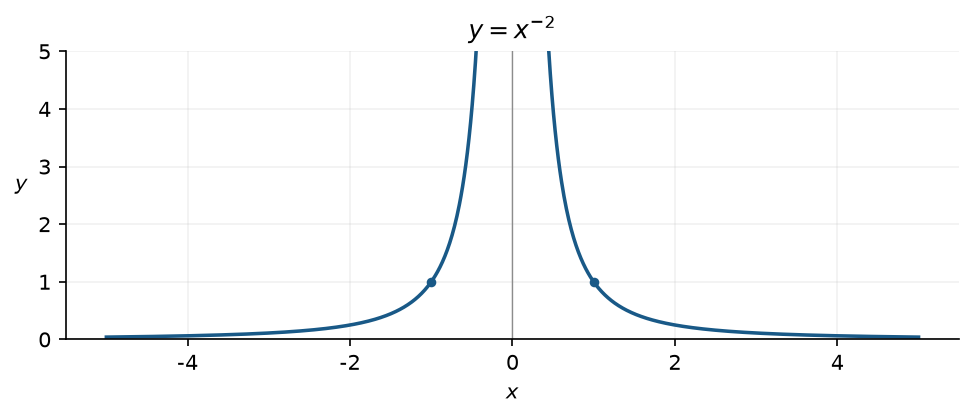
\includegraphics[width=.84\linewidth,height=.38\textheight,keepaspectratio]{figures/C04-PR103-3.png}\end{center}
{\small \field{关联知识}{P03 幂函数的概念、图象与性质（教材帮p.125、126、127 / PDF134、135、136）；F08 奇偶性、对称与函数性质应用（教材帮p.113、114、115 / PDF122、123、124）；F05 单调性定义、证明与参数（教材帮p.97、98、100 / PDF106、107、109）}
\field{方法与易错点}{设 $f(x)=x^\alpha$，用已知点求指数，再查该指数的定义域、奇偶性和各单调区间。 易错：把 $3x^2$ 当标准幂函数；将第一象限性质直接用于负半轴；分数负指数遗漏0禁点。}
\field{答案依据}{答案册相关题组：PDF第30、31页（册内页29、30）；按当前题库原题逐项重算，不按旧版题号机械对套。}}

\itemhead{p.103 练习 · 第4题（教材p.103）}{XJ-B1-C04-PR-P103-Y1471}
\label{XJ-B1-C04-PR-P103-Y1471}
{\footnotesize 湘教版教材p.103 / PDF第110页 / p.103 练习 / 第4题}
\field{原题}{已知幂函数 $m(x)$ 满足 $m(9)=27m(1)$，求 $m(25)$ 和 $m(8)$ 的值。}
\field{参考答案}{$m(1)=1$，$9^\alpha=27$ 得 $\alpha=3/2$；$m(25)=125,m(8)=16\sqrt2$。}
{\small \field{关联知识}{P03 幂函数的概念、图象与性质（教材帮p.125、126、127 / PDF134、135、136）}
\field{方法与易错点}{设 $f(x)=x^\alpha$，用已知点求指数，再查该指数的定义域、奇偶性和各单调区间。 易错：把 $3x^2$ 当标准幂函数；将第一象限性质直接用于负半轴；分数负指数遗漏0禁点。}
\field{答案依据}{答案册相关题组：PDF第30、31页（册内页29、30）；按当前题库原题逐项重算，不按旧版题号机械对套。}}

\itemhead{习题4.1 · 第1题（教材p.104）}{XJ-B1-C04-HW-P104-Y0450}
\label{XJ-B1-C04-HW-P104-Y0450}
{\footnotesize 湘教版教材p.104 / PDF第111页 / 习题4.1 / 第1题}
\field{原题}{求下列各式的值：
\subq{1}$\sqrt[3]{(-6)^3}$；
\subq{2}$\sqrt{(-7)^2}$；
\subq{3}$\sqrt[4]{(\sqrt2-2)^4}$；
\subq{4}$\sqrt[5]{(x-y)^5}$。}
\field{参考答案}{依次为 $-6,7,2-\sqrt2,x-y$。}
{\small \field{关联知识}{P01 方根、根式与绝对值（教材帮p.143 / PDF152）}
\field{方法与易错点}{先看根指数奇偶，再检查被开方数符号，必要时写绝对值分段。 易错：把偶次根式值写成正负两个；$\sqrt{a^2}$ 直接写 $a$。}
\field{答案依据}{答案册相关题组：PDF第31页（册内页30）；按当前题库原题逐项重算，不按旧版题号机械对套。}}

\itemhead{习题4.1 · 第2题（教材p.104）}{XJ-B1-C04-HW-P104-Y0598}
\label{XJ-B1-C04-HW-P104-Y0598}
{\footnotesize 湘教版教材p.104 / PDF第111页 / 习题4.1 / 第2题}
\field{原题}{用分数指数幂表示下列各式（式中字母都表示正数）：
\subq{1}$a\cdot\sqrt a\cdot\dfrac{a^2}{\sqrt{a\sqrt a}}$；
\subq{2}$\sqrt{\dfrac{a^3}b\sqrt{\dfrac{b^2}{a^6}}}$；
\subq{3}$\sqrt{2a^3b^5}\cdot\left(-6\sqrt a\cdot\sqrt[3]b\right)$。}
\field{参考答案}{依次为 $a^{11/4},1,-6\sqrt2\,a^2b^{17/6}$。按题库原式中根号及括号层次计算，结果与答案册原页一致。}
{\small \field{关联知识}{P02 有理数、实数指数幂与运算（教材帮p.144、145 / PDF153、154）}
\field{方法与易错点}{统一为指数幂，分开处理系数与各底数的指数；最终复查定义条件及数值精度。 易错：负指数误作负数；幂的幂指数相加；约分丢禁点；过早四舍五入。}
\field{答案依据}{答案册相关题组：PDF第31页（册内页30）；按当前题库原题逐项重算，不按旧版题号机械对套。}}

\itemhead{习题4.1 · 第3题（教材p.104）}{XJ-B1-C04-HW-P104-Y0788}
\label{XJ-B1-C04-HW-P104-Y0788}
{\footnotesize 湘教版教材p.104 / PDF第111页 / 习题4.1 / 第3题}
\field{原题}{用计算器计算下列各式的值（精确到 $0.001$）：
\subq{1}$7.2^{-1/3}$；
\subq{2}$4.7^{1/2}$；
\subq{3}$3^{\sqrt2}$。}
\field{参考答案}{依次约为0.518、2.168、4.729（精确到0.001）。}
{\small \field{关联知识}{P02 有理数、实数指数幂与运算（教材帮p.144、145 / PDF153、154）}
\field{方法与易错点}{统一为指数幂，分开处理系数与各底数的指数；最终复查定义条件及数值精度。 易错：负指数误作负数；幂的幂指数相加；约分丢禁点；过早四舍五入。}
\field{答案依据}{答案册相关题组：PDF第31页（册内页30）；按当前题库原题逐项重算，不按旧版题号机械对套。}}

\itemhead{习题4.1 · 第4题（教材p.104）}{XJ-B1-C04-HW-P104-Y0874}
\label{XJ-B1-C04-HW-P104-Y0874}
{\footnotesize 湘教版教材p.104 / PDF第111页 / 习题4.1 / 第4题}
\field{原题}{计算（式中字母都表示正数）：
\subq{1}$x^{1/3}\cdot x^{3/4}\cdot x^{-1/12}$；
\subq{2}$a^{3/2}\cdot a^{2/3}\cdot a^{-5/6}$；
\subq{3}$\left(x^{1/2}y^{-1/3}\right)^6$；
\subq{4}$\left(\dfrac{4s^2r^{-6}}{9t^4}\right)^{3/2}$；
\subq{5}$6x^{2/3}y^{-1/3}\div\left(\dfrac32x^{-4/3}y^{2/3}\right)$；
\subq{6}$\left(x^2-2+x^{-2}\right)\div\left(x^2-x^{-2}\right)$；
\subq{7}$\dfrac{x-y}{x^{2/3}+x^{1/3}y^{1/3}+y^{2/3}}$；
\subq{8}$\dfrac{a^{1/2}-b^{1/2}}{a^{1/2}+b^{1/2}}-\dfrac{a^{1/2}+b^{1/2}}{a^{1/2}-b^{1/2}}$。}
\field{参考答案}{依次为 $x,a^{4/3},x^3/y^2,8s^3/(27r^9t^6),4x^2/y,(x^2-1)/(x^2+1),x^{1/3}-y^{1/3},-4\sqrt{ab}/(a-b)$。第（6）仍须 $x\ne1$；第（8）须 $a\ne b$，均沿用原式限制。}
{\small \field{关联知识}{P02 有理数、实数指数幂与运算（教材帮p.144、145 / PDF153、154）；F02 定义域与原式限制（教材帮p.79、80、81 / PDF88、89、90）}
\field{方法与易错点}{统一为指数幂，分开处理系数与各底数的指数；最终复查定义条件及数值精度。 易错：负指数误作负数；幂的幂指数相加；约分丢禁点；过早四舍五入。}
\field{答案依据}{答案册相关题组：PDF第31页（册内页30）；按当前题库原题逐项重算，不按旧版题号机械对套。}}

\itemhead{习题4.1 · 第5题（教材p.104）}{XJ-B1-C04-HW-P104-Y1201}
\label{XJ-B1-C04-HW-P104-Y1201}
{\footnotesize 湘教版教材p.104 / PDF第111页 / 习题4.1 / 第5题}
\field{原题}{计算：
\[\sqrt[3]{2-\frac{62}{27}}+\sqrt{\left(-3\frac23\right)^2}-3\div16^{-0.75}+\sqrt[5]2\cdot\left(4^{-1/5}\right)^{-2}.\]}
\field{参考答案}{$-19$。四部分依次为 $-2/3,11/3,-24,2$。}
{\small \field{关联知识}{P02 有理数、实数指数幂与运算（教材帮p.144、145 / PDF153、154）}
\field{方法与易错点}{统一为指数幂，分开处理系数与各底数的指数；最终复查定义条件及数值精度。 易错：负指数误作负数；幂的幂指数相加；约分丢禁点；过早四舍五入。}
\field{答案依据}{答案册相关题组：PDF第31页（册内页30）；按当前题库原题逐项重算，不按旧版题号机械对套。}}

\itemhead{习题4.1 · 第6题（教材p.104）}{XJ-B1-C04-HW-P104-Y1259}
\label{XJ-B1-C04-HW-P104-Y1259}
{\footnotesize 湘教版教材p.104 / PDF第111页 / 习题4.1 / 第6题}
\field{原题}{化简：
\subq{1}$\left(\pi^{\sqrt2+1}\right)^{\sqrt2-1}$；
\subq{2}$\left(\left(\sqrt3\right)^{\sqrt[4]{64}}\right)^{\sqrt{25}}$。}
\field{参考答案}{（1）$\pi$；（2）$3^{5\sqrt2}$，因为 $\sqrt[4]{64}=2\sqrt2,\sqrt{25}=5$。以当前题库的根指数及括号为准。}
{\small \field{关联知识}{P02 有理数、实数指数幂与运算（教材帮p.144、145 / PDF153、154）}
\field{方法与易错点}{统一为指数幂，分开处理系数与各底数的指数；最终复查定义条件及数值精度。 易错：负指数误作负数；幂的幂指数相加；约分丢禁点；过早四舍五入。}
\field{答案依据}{答案册相关题组：PDF第31页（册内页30）；按当前题库原题逐项重算，不按旧版题号机械对套。}}

\itemhead{习题4.1 · 第7题（教材p.104）}{XJ-B1-C04-HW-P104-Y1352}
\label{XJ-B1-C04-HW-P104-Y1352}
{\footnotesize 湘教版教材p.104 / PDF第111页 / 习题4.1 / 第7题}
\field{原题}{比较下列各组中两个数的大小：
\subq{1}$3.5^{1.7}$ 与 $3.4^{1.7}$；
\subq{2}$3.5^{0.3}$ 与 $3.4^{0.3}$；
\subq{3}$3.5^{-1.6}$ 与 $3.4^{-1.6}$；
\subq{4}$0.12^{-0.6}$ 与 $0.11^{-0.6}$。}
\field{参考答案}{比较符号依次为 $>,>,<,<$；正指数保序，负指数反序。}
{\small \field{关联知识}{P03 幂函数的概念、图象与性质（教材帮p.125、126、127 / PDF134、135、136）}
\field{方法与易错点}{设 $f(x)=x^\alpha$，用已知点求指数，再查该指数的定义域、奇偶性和各单调区间。 易错：把 $3x^2$ 当标准幂函数；将第一象限性质直接用于负半轴；分数负指数遗漏0禁点。}
\field{答案依据}{答案册相关题组：PDF第31页（册内页30）；按当前题库原题逐项重算，不按旧版题号机械对套。}}

\itemhead{习题4.1 · 第8题（教材p.104）}{XJ-B1-C04-HW-P104-Y1494}
\label{XJ-B1-C04-HW-P104-Y1494}
{\footnotesize 湘教版教材p.104 / PDF第111页 / 习题4.1 / 第8题}
\field{原题}{已知幂函数 $f(x)=x^\alpha$ 的图象经过点 $\left(8,\dfrac12\right)$，求函数的表达式，并画出它的图象的草图，讨论它的奇偶性和单调性。}
\field{参考答案}{$f(x)=x^{-1/3}=1/\sqrt[3]x$，定义域 $\mathbb R\setminus\{0\}$，奇函数；在 $(-\infty,0)$、$(0,+\infty)$ 分别递减，无增区间；图象在第一、三象限，经过 $(1,1),(-1,-1)$。}
\begin{center}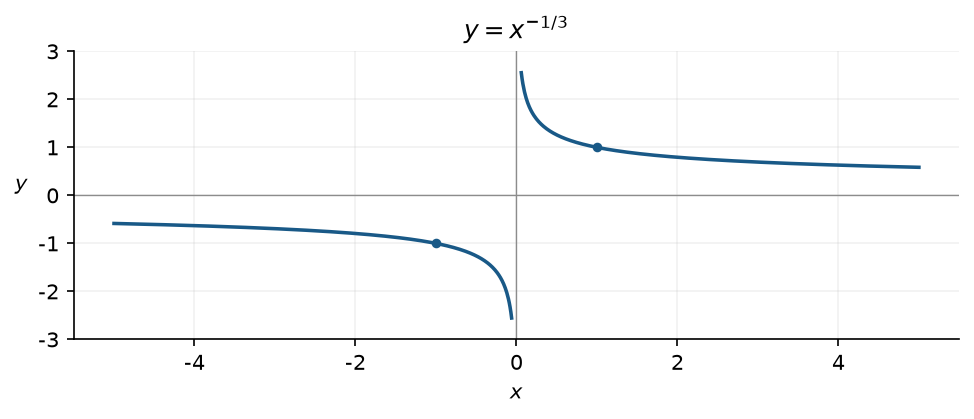
\includegraphics[width=.84\linewidth,height=.38\textheight,keepaspectratio]{figures/C04-HW104-8.png}\end{center}
{\small \field{关联知识}{P03 幂函数的概念、图象与性质（教材帮p.125、126、127 / PDF134、135、136）；F08 奇偶性、对称与函数性质应用（教材帮p.113、114、115 / PDF122、123、124）；F05 单调性定义、证明与参数（教材帮p.97、98、100 / PDF106、107、109）}
\field{方法与易错点}{设 $f(x)=x^\alpha$，用已知点求指数，再查该指数的定义域、奇偶性和各单调区间。 易错：把 $3x^2$ 当标准幂函数；将第一象限性质直接用于负半轴；分数负指数遗漏0禁点。}
\field{答案依据}{答案册相关题组：PDF第31页（册内页30）；按当前题库原题逐项重算，不按旧版题号机械对套。}}

\itemhead{习题4.1 · 第9题（教材p.105）}{XJ-B1-C04-HW-P105-Y0348}
\label{XJ-B1-C04-HW-P105-Y0348}
{\footnotesize 湘教版教材p.105 / PDF第112页 / 习题4.1 / 第9题}
\field{原题}{已知 $2^x+2^{-x}=5$，求 $4^x+\dfrac1{4^x}$ 的值。}
\field{参考答案}{23。将已知式平方：$4^x+4^{-x}+2=25$。}
{\small \field{关联知识}{P02 有理数、实数指数幂与运算（教材帮p.144、145 / PDF153、154）}
\field{方法与易错点}{统一为指数幂，分开处理系数与各底数的指数；最终复查定义条件及数值精度。 易错：负指数误作负数；幂的幂指数相加；约分丢禁点；过早四舍五入。}
\field{答案依据}{答案册相关题组：PDF第31页（册内页30）；按当前题库原题逐项重算，不按旧版题号机械对套。}}

\itemhead{习题4.1 · 第10题（教材p.105）}{XJ-B1-C04-HW-P105-Y0405}
\label{XJ-B1-C04-HW-P105-Y0405}
{\footnotesize 湘教版教材p.105 / PDF第112页 / 习题4.1 / 第10题}
\field{原题}{已知 $x>1$，且 $x+x^{-1}=3$，求下列各式的值：
\subq{1}$x^{1/2}+x^{-1/2}$；
\subq{2}$x^{1/2}-x^{-1/2}$；
\subq{3}$x^{3/2}+x^{-3/2}$。}
\field{参考答案}{依次为 $\sqrt5,1,2\sqrt5$。第二问由 $x>1$ 选正号；第三问用 $(u+v)^3-3uv(u+v)$，其中 $uv=1$。}
{\small \field{关联知识}{P02 有理数、实数指数幂与运算（教材帮p.144、145 / PDF153、154）}
\field{方法与易错点}{统一为指数幂，分开处理系数与各底数的指数；最终复查定义条件及数值精度。 易错：负指数误作负数；幂的幂指数相加；约分丢禁点；过早四舍五入。}
\field{答案依据}{答案册相关题组：PDF第31页（册内页30）；按当前题库原题逐项重算，不按旧版题号机械对套。}}

\itemhead{习题4.1 · 第11题（教材p.105）}{XJ-B1-C04-HW-P105-Y0490}
\label{XJ-B1-C04-HW-P105-Y0490}
{\footnotesize 湘教版教材p.105 / PDF第112页 / 习题4.1 / 第11题}
\field{原题}{已知 $f(x)$ 是奇函数，且当 $x\ge0$ 时，$f(x)=x^{2/5}$，求当 $x<0$ 时 $f(x)$ 的表达式。}
\field{参考答案}{$x<0$ 时 $f(x)=-f(-x)=-(-x)^{2/5}=-|x|^{2/5}$，不能漏负号。}
{\small \field{关联知识}{F08 奇偶性、对称与函数性质应用（教材帮p.113、114、115 / PDF122、123、124）；P03 幂函数的概念、图象与性质（教材帮p.125、126、127 / PDF134、135、136）}
\field{方法与易错点}{检查定义域，再代入 $-x$；求另一侧解析式时同时写出 $-x$ 所在区间。 易错：只看公式不看定义域；用一对点证明奇偶；负半轴代换遗漏最外层负号。}
\field{答案依据}{答案册相关题组：PDF第31页（册内页30）；按当前题库原题逐项重算，不按旧版题号机械对套。}}

\itemhead{习题4.1 · 第12题（教材p.105）}{XJ-B1-C04-HW-P105-Y0578}
\label{XJ-B1-C04-HW-P105-Y0578}
{\footnotesize 湘教版教材p.105 / PDF第112页 / 习题4.1 / 第12题}
\field{原题}{已知 $a=2^{4/3}$，$b=3^{2/3}$，$c=25^{1/3}$，比较 $a,b,c$ 的大小。}
\field{参考答案}{$b<a<c$。均为正数，立方后比较 $9<16<25$。}
{\small \field{关联知识}{P03 幂函数的概念、图象与性质（教材帮p.125、126、127 / PDF134、135、136）}
\field{方法与易错点}{设 $f(x)=x^\alpha$，用已知点求指数，再查该指数的定义域、奇偶性和各单调区间。 易错：把 $3x^2$ 当标准幂函数；将第一象限性质直接用于负半轴；分数负指数遗漏0禁点。}
\field{答案依据}{答案册相关题组：PDF第31页（册内页30）；按当前题库原题逐项重算，不按旧版题号机械对套。}}

\itemhead{习题4.1 · 第13题（教材p.105）}{XJ-B1-C04-HW-P105-Y0620}
\label{XJ-B1-C04-HW-P105-Y0620}
{\footnotesize 湘教版教材p.105 / PDF第112页 / 习题4.1 / 第13题}
\field{原题}{已知幂函数 $f(x)=x^{2m^2-m-6}\ (m\in\mathbb Z)$ 在 $(0,+\infty)$ 上是减函数。
\subq{1}求 $f(x)$ 的表达式；
\subq{2}判断 $f(x)$ 的奇偶性和单调性；
\subq{3}求 $f(x)$ 的值域。}
\field{参考答案}{$2m^2-m-6<0$ 得 $-3/2<m<2$，整数 $m=-1,0,1$ 分别给指数 $-3,-6,-5$。$x^{-3},x^{-5}$ 为奇函数，在两半轴分别递减，值域 $\mathbb R\setminus\{0\}$；$x^{-6}$ 为偶函数，在负半轴递增、正半轴递减，值域 $(0,+\infty)$。三者定义域均排除0。}
{\small \field{关联知识}{P03 幂函数的概念、图象与性质（教材帮p.125、126、127 / PDF134、135、136）；F08 奇偶性、对称与函数性质应用（教材帮p.113、114、115 / PDF122、123、124）；F05 单调性定义、证明与参数（教材帮p.97、98、100 / PDF106、107、109）}
\field{方法与易错点}{设 $f(x)=x^\alpha$，用已知点求指数，再查该指数的定义域、奇偶性和各单调区间。 易错：把 $3x^2$ 当标准幂函数；将第一象限性质直接用于负半轴；分数负指数遗漏0禁点。}
\field{答案依据}{答案册相关题组：PDF第31页（册内页30）；按当前题库原题逐项重算，不按旧版题号机械对套。}}

\itemhead{4.2 思考 · 未编号题组（教材p.106）}{XJ-B1-C04-TH-P106-Y0720}
\label{XJ-B1-C04-TH-P106-Y0720}
{\footnotesize 湘教版教材p.106 / PDF第113页 / 4.2 思考 / 未编号题组}
\field{原题}{\subq{1}将一张纸对折一次得到2层，对折两次得到4层。对折 $x$ 次后，纸的层数 $y$ 与 $x$ 之间有什么关系？
\subq{2}《庄子》中说：“一尺之棰，日取其半，万世不竭。”若每天截取木棰的一半，剩余木棰的长度 $y$（尺）与截取的天数 $x$ 之间有什么关系？
\subq{3}上述两个关系有什么共同特征？}
\field{参考答案}{（1）$y=2^x$，$x\in\mathbb N$；（2）$y=(1/2)^x$，$x\in\mathbb N$，表示每天截取后剩余长度；（3）均为等时间间隔按固定正倍率变化的指数模型，离散情境中自变量取非负整数。}
{\small \field{关联知识}{E03 指数增长、衰减与实际模型（教材帮p.131、132、154 / PDF140、141、163）}
\field{方法与易错点}{确认初始量、时间单位、倍率与时刻起点，再代入或逐次比较阈值。 易错：把年折旧10\%写成乘0.1；“超过”用成“达到”；时间起点错一位；把衰减至接近0当实际为0。}
\field{答案依据}{答案册未提供本栏目的独立对应答案；依据原题、教材概念补写参考回应。开放性总结不设唯一数值答案。}}

\itemhead{4.2 例题 · 例题1（教材p.108）}{XJ-B1-C04-EX-P108-Y0177}
\label{XJ-B1-C04-EX-P108-Y0177}
{\footnotesize 湘教版教材p.108 / PDF第115页 / 4.2 例题 / 例题1}
\field{原题}{某公司为大力提升创新水平，计划逐年加大研发资金投入。当年投入的研发资金为3500万元，预计下一年（将其计划执行的第一年）投入4200万元。若增速不变，该公司第 $x$ 年投入的研发资金用函数 $G(x)=C\cdot a^x$ 近似表示，写出此函数的解析式，并估计计划执行的第8年投入的研发资金（$1.2^8\approx4.3$）。}
\field{参考答案}{$G(x)=3500\times1.2^x$；第8年约 $3500\times4.3=15050$ 万元。当前年为 $x=0$，下一年为 $x=1$。}
{\small \field{关联知识}{E03 指数增长、衰减与实际模型（教材帮p.131、132、154 / PDF140、141、163）；F03 函数求值、解析式与函数建模（教材帮p.80、87、88、89、90、131 / PDF89、96、97、98、99、140）}
\field{方法与易错点}{确认初始量、时间单位、倍率与时刻起点，再代入或逐次比较阈值。 易错：把年折旧10\%写成乘0.1；“超过”用成“达到”；时间起点错一位；把衰减至接近0当实际为0。}
\field{答案依据}{例题原解位置：湘教版教材p.108及题库原图；独立编写可编辑参考解答。答案册此部分主要收练习、习题，不伪造例题答案册位置。}}

\itemhead{4.2 例题 · 例题2（教材p.108）}{XJ-B1-C04-EX-P108-Y0840}
\label{XJ-B1-C04-EX-P108-Y0840}
{\footnotesize 湘教版教材p.108 / PDF第115页 / 4.2 例题 / 例题2}
\field{原题}{医学中常用的钴60射线穿过1 cm厚的铅板后，强度变为原来的0.568倍。穿过厚度为 $x$ cm的铅板后的强度与原来强度之比为 $H(x)=a^x$。若铅板厚度为12 cm，射线穿过铅板后的强度与原来强度之比是多少？}
\field{参考答案}{$a=0.568,H(x)=0.568^x$；$H(12)=0.568^{12}\approx0.001128$，约为原强度的 $0.1128\%$。}
{\small \field{关联知识}{E03 指数增长、衰减与实际模型（教材帮p.131、132、154 / PDF140、141、163）}
\field{方法与易错点}{确认初始量、时间单位、倍率与时刻起点，再代入或逐次比较阈值。 易错：把年折旧10\%写成乘0.1；“超过”用成“达到”；时间起点错一位；把衰减至接近0当实际为0。}
\field{答案依据}{例题原解位置：湘教版教材p.108及题库原图；独立编写可编辑参考解答。答案册此部分主要收练习、习题，不伪造例题答案册位置。}}

\itemhead{p.108 练习 · 第1题（教材p.108）}{XJ-B1-C04-PR-P108-Y1273}
\label{XJ-B1-C04-PR-P108-Y1273}
{\footnotesize 湘教版教材p.108 / PDF第115页 / p.108 练习 / 第1题}
\field{原题}{某种细胞每小时分裂一次，由1个分裂成2个。若开始有1个细胞，经过 $x$ 小时后细胞的总数为 $y$，写出 $y$ 与 $x$ 之间的函数表达式；细胞总数超过2048个，至少需要几小时？}
\field{参考答案}{$y=2^x$，$x\in\mathbb N$。$2^{11}=2048$，严格超过需至少12小时。}
{\small \field{关联知识}{E03 指数增长、衰减与实际模型（教材帮p.131、132、154 / PDF140、141、163）}
\field{方法与易错点}{确认初始量、时间单位、倍率与时刻起点，再代入或逐次比较阈值。 易错：把年折旧10\%写成乘0.1；“超过”用成“达到”；时间起点错一位；把衰减至接近0当实际为0。}
\field{答案依据}{答案册相关题组：PDF第31页（册内页30）；按当前题库原题逐项重算，不按旧版题号机械对套。}}

\itemhead{p.108 练习 · 第2题（教材p.108）}{XJ-B1-C04-PR-P108-Y1402}
\label{XJ-B1-C04-PR-P108-Y1402}
{\footnotesize 湘教版教材p.108 / PDF第115页 / p.108 练习 / 第2题}
\field{原题}{氡是一种放射性元素，它的半衰期为3.82天。
\subq{1}经过7.64天，氡是否全部消失？
\subq{2}经过多少天，氡的剩余量为原来的 $\dfrac18$？}
\field{参考答案}{（1）没有，剩余原来的 $1/4$；（2）$3\times3.82=11.46$ 天。}
{\small \field{关联知识}{E03 指数增长、衰减与实际模型（教材帮p.131、132、154 / PDF140、141、163）}
\field{方法与易错点}{确认初始量、时间单位、倍率与时刻起点，再代入或逐次比较阈值。 易错：把年折旧10\%写成乘0.1；“超过”用成“达到”；时间起点错一位；把衰减至接近0当实际为0。}
\field{答案依据}{答案册相关题组：PDF第31页（册内页30）；按当前题库原题逐项重算，不按旧版题号机械对套。}}

\itemhead{4.2 思考 · 未编号题组（教材p.109）}{XJ-B1-C04-TH-P109-Y0302}
\label{XJ-B1-C04-TH-P109-Y0302}
{\footnotesize 湘教版教材p.109 / PDF第116页 / 4.2 思考 / 未编号题组}
\field{原题}{观察函数 $y=2^x$ 和 $y=\left(\dfrac12\right)^x$ 的下列函数值表：
\[\begin{array}{c|rrrrrrr}
x&-100&-10&-5&0&5&10&100\\\hline
2^x&2^{-100}&2^{-10}&1/32&1&32&2^{10}&2^{100}\\
(1/2)^x&2^{100}&2^{10}&32&1&1/32&2^{-10}&2^{-100}
\end{array}\]
\subq{1}观察这些函数值，猜想这两个函数的值域和单调性。
\subq{2}这些猜想能否推广为函数 $y=a^x\ (a>0,\ a\ne1)$ 的性质？}
\field{参考答案}{两函数值域均为 $(0,+\infty)$，$2^x$ 在 $\mathbb R$ 递增，$(1/2)^x$ 递减。一般地，$a>1$ 递增，$0<a<1$ 递减；定义域均为 $\mathbb R$，恒过 $(0,1)$，不取0。}
{\small \field{关联知识}{E01 指数函数的概念、图象与性质（教材帮p.150、151 / PDF159、160）}
\field{方法与易错点}{先查底数条件，利用已知点定底数，再据单调性及图象求值或范围。 易错：只要求底数非负；漏排1；将 $a^x+b$ 当标准指数函数且仍用原值域。}
\field{答案依据}{答案册未提供本栏目的独立对应答案；依据原题、教材概念补写参考回应。开放性总结不设唯一数值答案。}}

\itemhead{4.2 例题 · 例题3（教材p.110）}{XJ-B1-C04-EX-P110-Y0319}
\label{XJ-B1-C04-EX-P110-Y0319}
{\footnotesize 湘教版教材p.110 / PDF第117页 / 4.2 例题 / 例题3}
\field{原题}{作出指数函数 $y=3^x$ 和 $y=10^x$ 的图象。}
\field{参考答案}{分别标点：$3^x$ 经过 $(-1,1/3),(0,1),(1,3)$；$10^x$ 经过 $(-1,1/10),(0,1),(1,10)$，用递增平滑曲线连接，向左逼近 $x$ 轴。$x>0$ 时 $10^x>3^x$；$x<0$ 时反向。}
\begin{center}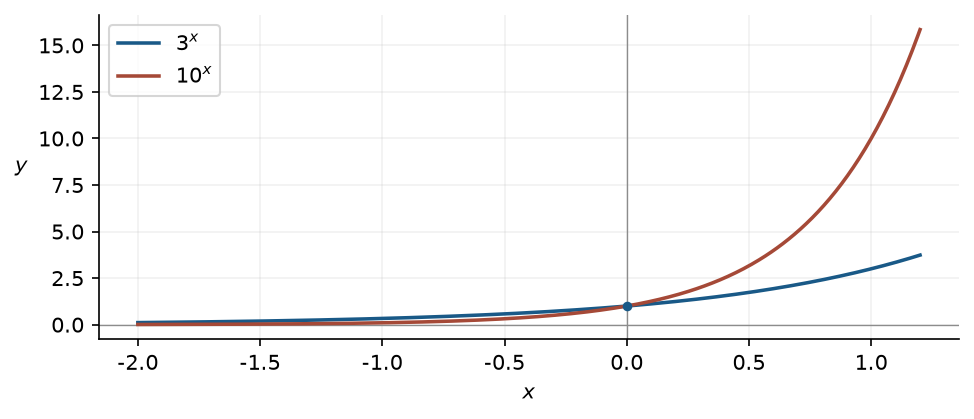
\includegraphics[width=.84\linewidth,height=.38\textheight,keepaspectratio]{figures/C04-EX110-3.png}\end{center}
{\small \field{关联知识}{E01 指数函数的概念、图象与性质（教材帮p.150、151 / PDF159、160）；F04 函数三种表示法、图象与读数（教材帮p.85、86、93、94 / PDF94、95、102、103）}
\field{方法与易错点}{先查底数条件，利用已知点定底数，再据单调性及图象求值或范围。 易错：只要求底数非负；漏排1；将 $a^x+b$ 当标准指数函数且仍用原值域。}
\field{答案依据}{例题原解位置：湘教版教材p.110及题库原图；独立编写可编辑参考解答。答案册此部分主要收练习、习题，不伪造例题答案册位置。}}

\itemhead{4.2 思考 · 未编号题组（教材p.110）}{XJ-B1-C04-TH-P110-Y1359}
\label{XJ-B1-C04-TH-P110-Y1359}
{\footnotesize 湘教版教材p.110 / PDF第117页 / 4.2 思考 / 未编号题组}
\field{原题}{当 $a>1$ 时，$y=a^x$ 和 $y=\left(\dfrac1a\right)^x$ 的图象有什么关系？能否利用 $y=a^x$ 的图象画出 $y=\left(\dfrac1a\right)^x$ 的图象？}
\field{参考答案}{两图象关于 $y$ 轴对称，因为 $(1/a)^x=a^{-x}$；将每个点 $(x,a^x)$ 映到 $(-x,a^x)$ 即得。}
{\small \field{关联知识}{E01 指数函数的概念、图象与性质（教材帮p.150、151 / PDF159、160）；F09 图象平移、伸缩与对称（教材帮p.86、94 / PDF95、103）}
\field{方法与易错点}{先查底数条件，利用已知点定底数，再据单调性及图象求值或范围。 易错：只要求底数非负；漏排1；将 $a^x+b$ 当标准指数函数且仍用原值域。}
\field{答案依据}{答案册未提供本栏目的独立对应答案；依据原题、教材概念补写参考回应。开放性总结不设唯一数值答案。}}

\itemhead{4.2 例题 · 例题4（教材p.111）}{XJ-B1-C04-EX-P111-Y1422}
\label{XJ-B1-C04-EX-P111-Y1422}
{\footnotesize 湘教版教材p.111 / PDF第118页 / 4.2 例题 / 例题4}
\field{原题}{比较下列各组中两个数的大小：
\subq{1}$3.5^{1.5}$ 与 $3.5^{1.3}$；
\subq{2}$0.3^{1.5}$ 与 $0.3^{1.3}$；
\subq{3}$0.7^{0.8}$ 与 $0.8^{0.7}$。}
\field{参考答案}{符号依次为 $>,<,<$。（3）$0.7^{0.8}<0.8^{0.8}<0.8^{0.7}$，分别比较同指数的底数与同底数的指数。}
{\small \field{关联知识}{E02 指数式比较、方程与不等式（教材帮p.154、155 / PDF163、164）；P03 幂函数的概念、图象与性质（教材帮p.125、126、127 / PDF134、135、136）}
\field{方法与易错点}{将比较对象化成同底、同指数，或加入合适中间量；解后复查范围。 易错：所有底数都按递增；底数和指数同时变化时凭直觉判断。}
\field{答案依据}{例题原解位置：湘教版教材p.111及题库原图；独立编写可编辑参考解答。答案册此部分主要收练习、习题，不伪造例题答案册位置。}}

\itemhead{4.2 例题 · 例题5（教材p.112）}{XJ-B1-C04-EX-P112-Y0737}
\label{XJ-B1-C04-EX-P112-Y0737}
{\footnotesize 湘教版教材p.112 / PDF第119页 / 4.2 例题 / 例题5}
\field{原题}{已知指数函数 $f(x)=a^x$ 的图象经过点 $(2,7)$，求 $f(-6)$ 和 $f(3)$ 的值。}
\field{参考答案}{$a=\sqrt7$，$f(-6)=1/343$，$f(3)=7\sqrt7$。}
{\small \field{关联知识}{E01 指数函数的概念、图象与性质（教材帮p.150、151 / PDF159、160）；P02 有理数、实数指数幂与运算（教材帮p.144、145 / PDF153、154）}
\field{方法与易错点}{先查底数条件，利用已知点定底数，再据单调性及图象求值或范围。 易错：只要求底数非负；漏排1；将 $a^x+b$ 当标准指数函数且仍用原值域。}
\field{答案依据}{例题原解位置：湘教版教材p.112及题库原图；独立编写可编辑参考解答。答案册此部分主要收练习、习题，不伪造例题答案册位置。}}

\itemhead{4.2 例题 · 例题6（教材p.112）}{XJ-B1-C04-EX-P112-Y1015}
\label{XJ-B1-C04-EX-P112-Y1015}
{\footnotesize 湘教版教材p.112 / PDF第119页 / 4.2 例题 / 例题6}
\field{原题}{某种放射性物质每年剩余量是上一年的84\%。画出这种物质的剩余量与时间的函数图象，并由图象读出经过多少年剩余量约为原来的50\%。}
\field{参考答案}{设原量为 $M_0$，$M(t)=M_0\times0.84^t$，$t\ge0$；$0.84^4\approx0.498$，约4年剩余50\%。图象从 $(0,M_0)$ 起递减且始终大于0。}
\begin{center}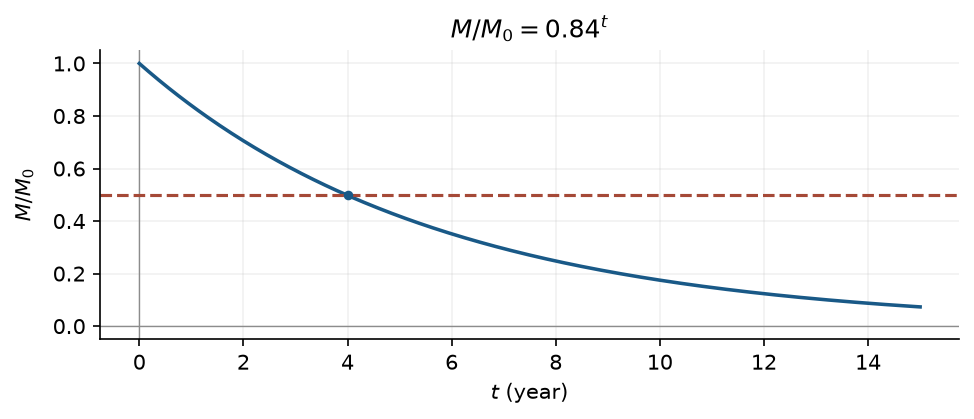
\includegraphics[width=.84\linewidth,height=.38\textheight,keepaspectratio]{figures/C04-EX112-6.png}\end{center}
{\small \field{关联知识}{E03 指数增长、衰减与实际模型（教材帮p.131、132、154 / PDF140、141、163）；F04 函数三种表示法、图象与读数（教材帮p.85、86、93、94 / PDF94、95、102、103）}
\field{方法与易错点}{确认初始量、时间单位、倍率与时刻起点，再代入或逐次比较阈值。 易错：把年折旧10\%写成乘0.1；“超过”用成“达到”；时间起点错一位；把衰减至接近0当实际为0。}
\field{答案依据}{例题原解位置：湘教版教材p.112及题库原图；独立编写可编辑参考解答。答案册此部分主要收练习、习题，不伪造例题答案册位置。}}

\itemhead{p.113 练习 · 第1题（教材p.113）}{XJ-B1-C04-PR-P113-Y0217}
\label{XJ-B1-C04-PR-P113-Y0217}
{\footnotesize 湘教版教材p.113 / PDF第120页 / p.113 练习 / 第1题}
\field{原题}{在同一平面直角坐标系中画出 $y=5^x$ 和 $y=5^{-x}$ 的图象，并说明它们之间的关系。}
\field{参考答案}{$5^x$ 与 $5^{-x}$ 均过 $(0,1)$，前者递增后者递减，关于 $y$ 轴对称。取 $x=-1,0,1$ 时函数值分别为 $1/5,1,5$ 与 $5,1,1/5$。}
\begin{center}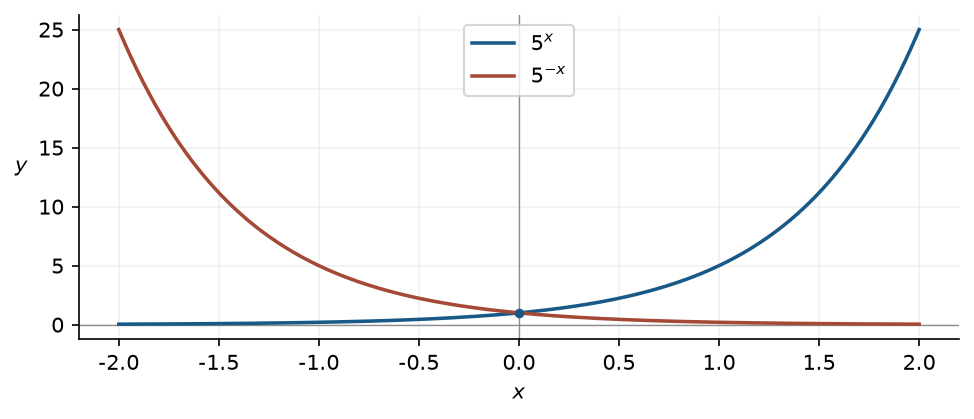
\includegraphics[width=.84\linewidth,height=.38\textheight,keepaspectratio]{figures/C04-PR113-1.png}\end{center}
\field{核对说明}{底数变化：答案册PDF31标p.112并作3\textasciicircum{}x图象；现教材p.113为5\textasciicircum{}x和5\textasciicircum{}(-x)，对称关系相同，作图点值必须更新。}
{\small \field{关联知识}{E01 指数函数的概念、图象与性质（教材帮p.150、151 / PDF159、160）；F09 图象平移、伸缩与对称（教材帮p.86、94 / PDF95、103）}
\field{方法与易错点}{先查底数条件，利用已知点定底数，再据单调性及图象求值或范围。 易错：只要求底数非负；漏排1；将 $a^x+b$ 当标准指数函数且仍用原值域。}
\field{答案依据}{答案册相关题组：PDF第31页（册内页30）；按当前题库原题逐项重算，不按旧版题号机械对套。}}

\itemhead{p.113 练习 · 第2题（教材p.113）}{XJ-B1-C04-PR-P113-Y0303}
\label{XJ-B1-C04-PR-P113-Y0303}
{\footnotesize 湘教版教材p.113 / PDF第120页 / p.113 练习 / 第2题}
\field{原题}{已知指数函数 $f(x)=a^x$ 的图象经过点 $(2,2)$，求 $f(1)$ 的值。}
\field{参考答案}{$a^2=2,a>0$，得 $f(1)=a=\sqrt2$。}
{\small \field{关联知识}{E01 指数函数的概念、图象与性质（教材帮p.150、151 / PDF159、160）}
\field{方法与易错点}{先查底数条件，利用已知点定底数，再据单调性及图象求值或范围。 易错：只要求底数非负；漏排1；将 $a^x+b$ 当标准指数函数且仍用原值域。}
\field{答案依据}{答案册相关题组：PDF第31页（册内页30）；按当前题库原题逐项重算，不按旧版题号机械对套。}}

\itemhead{p.113 练习 · 第3题（教材p.113）}{XJ-B1-C04-PR-P113-Y0347}
\label{XJ-B1-C04-PR-P113-Y0347}
{\footnotesize 湘教版教材p.113 / PDF第120页 / p.113 练习 / 第3题}
\field{原题}{比较下列各组中两个数的大小：
\subq{1}$0.2^{0.3}$ 与 $0.2^{0.2}$；
\subq{2}$1.2^{0.3}$ 与 $1.2^{0.2}$；
\subq{3}$0.3^{0.1}$ 与 $0.3^{-0.1}$；
\subq{4}$1.35^{0.2}$ 与 $1.35^{-0.2}$。}
\field{参考答案}{比较符号依次为 $<,>,<,>$。}
{\small \field{关联知识}{E02 指数式比较、方程与不等式（教材帮p.154、155 / PDF163、164）}
\field{方法与易错点}{将比较对象化成同底、同指数，或加入合适中间量；解后复查范围。 易错：所有底数都按递增；底数和指数同时变化时凭直觉判断。}
\field{答案依据}{答案册相关题组：PDF第31页（册内页30）；按当前题库原题逐项重算，不按旧版题号机械对套。}}

\itemhead{p.113 练习 · 第4题（教材p.113）}{XJ-B1-C04-PR-P113-Y0475}
\label{XJ-B1-C04-PR-P113-Y0475}
{\footnotesize 湘教版教材p.113 / PDF第120页 / p.113 练习 / 第4题}
\field{原题}{求函数 $y=2^{|3-x|}$ 的值域。}
\field{参考答案}{$[1,+\infty)$。$|3-x|\ge0$，最小指数0在 $x=3$ 取到。}
{\small \field{关联知识}{E01 指数函数的概念、图象与性质（教材帮p.150、151 / PDF159、160）；F06 最大值、最小值与值域（教材帮p.99、83、84 / PDF108、92、93）}
\field{方法与易错点}{先查底数条件，利用已知点定底数，再据单调性及图象求值或范围。 易错：只要求底数非负；漏排1；将 $a^x+b$ 当标准指数函数且仍用原值域。}
\field{答案依据}{答案册相关题组：PDF第31页（册内页30）；按当前题库原题逐项重算，不按旧版题号机械对套。}}

\itemhead{习题4.2 · 第1题（教材p.113）}{XJ-B1-C04-HW-P113-Y0886}
\label{XJ-B1-C04-HW-P113-Y0886}
{\footnotesize 湘教版教材p.113 / PDF第120页 / 习题4.2 / 第1题}
\field{原题}{设 $f(x)=2^x$，计算 $f(0)-f(-1)$，$f(2)-f(1)$，$f(4)-f(3)$，$f(6)-f(5)$。比较这些差的大小，你有什么发现？}
\field{参考答案}{四个差依次为 $1/2,2,8,32$，逐渐增大；一般 $f(n+1)-f(n)=2^n$，相邻单位区间的增长量随 $n$ 增大而增大。}
{\small \field{关联知识}{E01 指数函数的概念、图象与性质（教材帮p.150、151 / PDF159、160）；P02 有理数、实数指数幂与运算（教材帮p.144、145 / PDF153、154）}
\field{方法与易错点}{先查底数条件，利用已知点定底数，再据单调性及图象求值或范围。 易错：只要求底数非负；漏排1；将 $a^x+b$ 当标准指数函数且仍用原值域。}
\field{答案依据}{答案册相关题组：PDF第32页（册内页31）；按当前题库原题逐项重算，不按旧版题号机械对套。}}

\itemhead{习题4.2 · 第2题（教材p.113）}{XJ-B1-C04-HW-P113-Y1057}
\label{XJ-B1-C04-HW-P113-Y1057}
{\footnotesize 湘教版教材p.113 / PDF第120页 / 习题4.2 / 第2题}
\field{原题}{某林区的木材蓄积量每年增长12\%。经过 $x$ 年后，木材蓄积量为原来的 $y$ 倍，求 $y$ 与 $x$ 之间的函数表达式。}
\field{参考答案}{$y=1.12^x$，通常 $x\in\mathbb N$。每年增长12\%，故每年的倍率为1.12。}
{\small \field{关联知识}{E03 指数增长、衰减与实际模型（教材帮p.131、132、154 / PDF140、141、163）}
\field{方法与易错点}{确认初始量、时间单位、倍率与时刻起点，再代入或逐次比较阈值。 易错：把年折旧10\%写成乘0.1；“超过”用成“达到”；时间起点错一位；把衰减至接近0当实际为0。}
\field{答案依据}{答案册相关题组：PDF第32页（册内页31）；按当前题库原题逐项重算，不按旧版题号机械对套。}}

\itemhead{习题4.2 · 第3题（教材p.113）}{XJ-B1-C04-HW-P113-Y1144}
\label{XJ-B1-C04-HW-P113-Y1144}
{\footnotesize 湘教版教材p.113 / PDF第120页 / 习题4.2 / 第3题}
\field{原题}{一辆新车的售价为16万元，使用 $x$ 年后，其价值 $P$（万元）为 $P=16\cdot0.9^x$。
\subq{1}说明式中0.9的含义；
\subq{2}求这辆车使用3年、9年后的价值。}
\field{参考答案}{（1）每年的保留价值为前一年的90\%，年折旧率10\%；（2）$P(3)=11.664$ 万元，$P(9)=6.198727824\approx6.20$ 万元。}
\field{核对说明}{近似值差异：16×0.9\textasciicircum{}9=6.198727824万元，通常保留两位小数为6.20；答案册PDF32写约6.19，现采用精确值舍入。}
{\small \field{关联知识}{E03 指数增长、衰减与实际模型（教材帮p.131、132、154 / PDF140、141、163）}
\field{方法与易错点}{确认初始量、时间单位、倍率与时刻起点，再代入或逐次比较阈值。 易错：把年折旧10\%写成乘0.1；“超过”用成“达到”；时间起点错一位；把衰减至接近0当实际为0。}
\field{答案依据}{答案册相关题组：PDF第32页（册内页31）；按当前题库原题逐项重算，不按旧版题号机械对套。}}

\itemhead{习题4.2 · 第4题（教材p.113）}{XJ-B1-C04-HW-P113-Y1315}
\label{XJ-B1-C04-HW-P113-Y1315}
{\footnotesize 湘教版教材p.113 / PDF第120页 / 习题4.2 / 第4题}
\field{原题}{食品的保鲜时间 $y$（h）与温度 $x$（$^\circ\mathrm C$）的关系为 $y=\mathrm e^{kx+b}$，其中 $\mathrm e=2.71828\cdots$，$k,b$ 为常数。某种食品在 $0\,{}^\circ\mathrm C$ 时保鲜时间为192 h，在 $22\,{}^\circ\mathrm C$ 时保鲜时间为48 h，求该食品在 $33\,{}^\circ\mathrm C$ 时的保鲜时间。}
\field{参考答案}{由 $e^b=192,e^{22k}=48/192=1/4$，得 $e^{33k}=(1/4)^{3/2}=1/8$；故33摄氏度时为24小时。无需使用对数。}
{\small \field{关联知识}{E03 指数增长、衰减与实际模型（教材帮p.131、132、154 / PDF140、141、163）；P02 有理数、实数指数幂与运算（教材帮p.144、145 / PDF153、154）}
\field{方法与易错点}{确认初始量、时间单位、倍率与时刻起点，再代入或逐次比较阈值。 易错：把年折旧10\%写成乘0.1；“超过”用成“达到”；时间起点错一位；把衰减至接近0当实际为0。}
\field{答案依据}{答案册相关题组：PDF第32页（册内页31）；按当前题库原题逐项重算，不按旧版题号机械对套。}}

\itemhead{习题4.2 · 第5题（教材p.113）}{XJ-B1-C04-HW-P113-Y1446}
\label{XJ-B1-C04-HW-P113-Y1446}
{\footnotesize 湘教版教材p.113 / PDF第120页 / 习题4.2 / 第5题}
\field{原题}{求下列函数的定义域：
\subq{1}$y=8^{\frac1{3x-1}}$；
\subq{2}$y=\sqrt{1-\left(\dfrac16\right)^x}$。}
\field{参考答案}{（1）$\mathbb R\setminus\{1/3\}$；（2）$[0,+\infty)$，因为 $(1/6)^x\le1$ 当且仅当 $x\ge0$。}
{\small \field{关联知识}{F02 定义域与原式限制（教材帮p.79、80、81 / PDF88、89、90）；E01 指数函数的概念、图象与性质（教材帮p.150、151 / PDF159、160）}
\field{方法与易错点}{按原式逐项列条件后求交集，不先约分再判断。 易错：遗漏分母禁点；将函数值范围错当自变量范围；把退化矩形算入实际定义域。}
\field{答案依据}{答案册相关题组：PDF第32页（册内页31）；按当前题库原题逐项重算，不按旧版题号机械对套。}}

\itemhead{习题4.2 · 第6题（教材p.113）}{XJ-B1-C04-HW-P113-Y1566}
\label{XJ-B1-C04-HW-P113-Y1566}
{\footnotesize 湘教版教材p.113 / PDF第120页 / 习题4.2 / 第6题}
\field{原题}{在同一平面直角坐标系中画出 $y=4^x$，$y=4^{-x}$，$y=4^{x+1}$，$y=4^{x-1}$ 的图象，并说明后三个函数的图象分别可以由第一个函数的图象怎样变换得到。}
\field{参考答案}{后三图依次由 $4^x$ 关于 $y$ 轴对称、向左平移1、向右平移1得到；可各取三点 $x=-1,0,1$ 求值画图，均保持正函数值。}
\begin{center}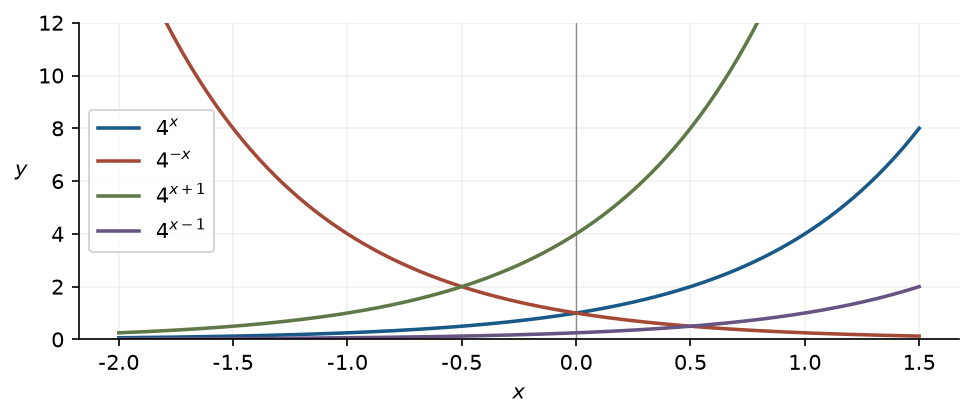
\includegraphics[width=.84\linewidth,height=.38\textheight,keepaspectratio]{figures/C04-HW113-6.png}\end{center}
{\small \field{关联知识}{F09 图象平移、伸缩与对称（教材帮p.86、94 / PDF95、103）；E01 指数函数的概念、图象与性质（教材帮p.150、151 / PDF159、160）}
\field{方法与易错点}{追踪点 $(u,f(u))$ 变换后的坐标，反推新解析式。 易错：平移只改公式而未改定义域；把纵向倍率当作指数底数变化。}
\field{答案依据}{答案册相关题组：PDF第32页（册内页31）；按当前题库原题逐项重算，不按旧版题号机械对套。}}

\itemhead{习题4.2 · 第7题（教材p.114）}{XJ-B1-C04-HW-P114-Y0303}
\label{XJ-B1-C04-HW-P114-Y0303}
{\footnotesize 湘教版教材p.114 / PDF第121页 / 习题4.2 / 第7题}
\field{原题}{已知 $a,b,c,d$ 为不等于1的正数。图中为 $y=a^x$，$y=b^x$，$y=c^x$，$y=d^x$ 的图象，比较 $a,b,c,d$ 的大小：\blank。
\bankfig{C04-HW114}{0.55}}
\field{参考答案}{$b<a<1<d<c$，故填 $b<a<d<c$。在 $x=1$ 处读取函数值就是各底数；负半轴图象的上下关系相反。}
{\small \field{关联知识}{E01 指数函数的概念、图象与性质（教材帮p.150、151 / PDF159、160）；F04 函数三种表示法、图象与读数（教材帮p.85、86、93、94 / PDF94、95、102、103）}
\field{方法与易错点}{先查底数条件，利用已知点定底数，再据单调性及图象求值或范围。 易错：只要求底数非负；漏排1；将 $a^x+b$ 当标准指数函数且仍用原值域。}
\field{答案依据}{答案册相关题组：PDF第32页（册内页31）；按当前题库原题逐项重算，不按旧版题号机械对套。}}

\itemhead{习题4.2 · 第8题（教材p.114）}{XJ-B1-C04-HW-P114-Y0667}
\label{XJ-B1-C04-HW-P114-Y0667}
{\footnotesize 湘教版教材p.114 / PDF第121页 / 习题4.2 / 第8题}
\field{原题}{已知 $0<a<1$，$b<-1$，函数 $y=a^x+b$ 的图象不经过哪个象限？}
\field{参考答案}{不经过第一象限。$x\ge0$ 时 $a^x\le1$，故 $a^x+b<0$；在负半轴既有正值也有负值，因此其余三个象限均经过。}
{\small \field{关联知识}{E01 指数函数的概念、图象与性质（教材帮p.150、151 / PDF159、160）；F09 图象平移、伸缩与对称（教材帮p.86、94 / PDF95、103）}
\field{方法与易错点}{先查底数条件，利用已知点定底数，再据单调性及图象求值或范围。 易错：只要求底数非负；漏排1；将 $a^x+b$ 当标准指数函数且仍用原值域。}
\field{答案依据}{答案册相关题组：PDF第32页（册内页31）；按当前题库原题逐项重算，不按旧版题号机械对套。}}

\itemhead{习题4.2 · 第9题（教材p.114）}{XJ-B1-C04-HW-P114-Y0711}
\label{XJ-B1-C04-HW-P114-Y0711}
{\footnotesize 湘教版教材p.114 / PDF第121页 / 习题4.2 / 第9题}
\field{原题}{比较下列各组中两个数的大小：
\subq{1}$0.6^{-0.1}$ 与 $0.6^{-0.5}$；
\subq{2}$1.6^{2.5}$ 与 $1.7^3$；
\subq{3}$1.7^{0.3}$ 与 $0.9^{3.1}$。}
\field{参考答案}{比较符号依次为 $<,<,>$。（2）$1.6^{2.5}<1.7^{2.5}<1.7^3$；（3）左大于1，右小于1。}
{\small \field{关联知识}{E02 指数式比较、方程与不等式（教材帮p.154、155 / PDF163、164）；P03 幂函数的概念、图象与性质（教材帮p.125、126、127 / PDF134、135、136）}
\field{方法与易错点}{将比较对象化成同底、同指数，或加入合适中间量；解后复查范围。 易错：所有底数都按递增；底数和指数同时变化时凭直觉判断。}
\field{答案依据}{答案册相关题组：PDF第32页（册内页31）；按当前题库原题逐项重算，不按旧版题号机械对套。}}

\itemhead{习题4.2 · 第10题（教材p.114）}{XJ-B1-C04-HW-P114-Y0935}
\label{XJ-B1-C04-HW-P114-Y0935}
{\footnotesize 湘教版教材p.114 / PDF第121页 / 习题4.2 / 第10题}
\field{原题}{用图象法判断函数 $y=2^x$ 与 $y=x^2$ 的图象有几个交点，并用计算机验证。}
\field{参考答案}{有3个交点，横坐标约为 $-0.766665,2,4$。两个正根可直接代入；负根可用二分数值法定位。用作图或计算机验证时须在负半轴、正半轴均查看，不能只数2、4。}
\begin{center}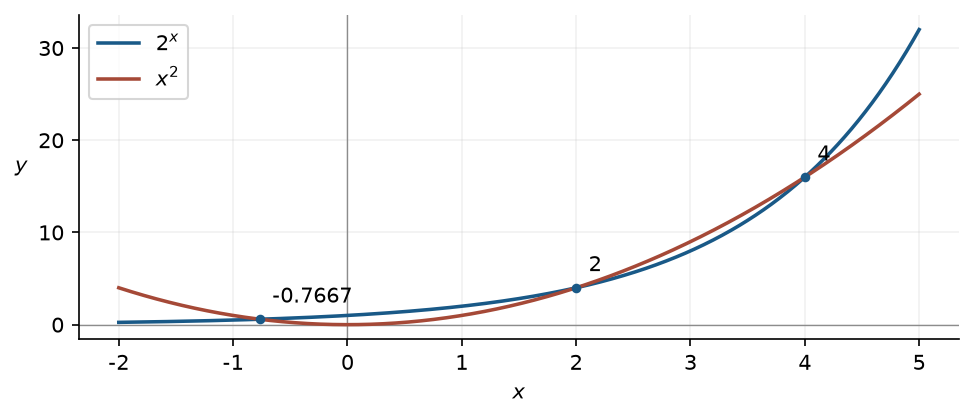
\includegraphics[width=.84\linewidth,height=.38\textheight,keepaspectratio]{figures/C04-HW114-10.png}\end{center}
{\small \field{关联知识}{F04 函数三种表示法、图象与读数（教材帮p.85、86、93、94 / PDF94、95、102、103）；E01 指数函数的概念、图象与性质（教材帮p.150、151 / PDF159、160）}
\field{方法与易错点}{把关键点与定义域一起标到图上，逐区间读交点和上下关系。 易错：将示意图预测当事实；把两曲线交点收进严格不等式；折线漏端点。}
\field{答案依据}{答案册相关题组：PDF第32页（册内页31）；按当前题库原题逐项重算，不按旧版题号机械对套。}}

\itemhead{习题4.2 · 第11题（教材p.114）}{XJ-B1-C04-HW-P114-Y1038}
\label{XJ-B1-C04-HW-P114-Y1038}
{\footnotesize 湘教版教材p.114 / PDF第121页 / 习题4.2 / 第11题}
\field{原题}{已知函数 $f(x)=a^{|3x-1|}\ (a>0,\ a\ne1)$，且 $f(1)=\dfrac49$。
\subq{1}求 $a$ 的值；
\subq{2}讨论 $f(x)$ 的单调性；
\subq{3}求 $f(x)$ 的值域。}
\field{参考答案}{（1）$a^2=4/9$ 得 $a=2/3$；（2）在 $(-\infty,1/3]$ 递增，在 $[1/3,+\infty)$ 递减；（3）值域 $(0,1]$。}
{\small \field{关联知识}{E01 指数函数的概念、图象与性质（教材帮p.150、151 / PDF159、160）；F07 分段函数、绝对值及分段应用（教材帮p.86、91、92、93 / PDF95、100、101、102）；F06 最大值、最小值与值域（教材帮p.99、83、84 / PDF108、92、93）}
\field{方法与易错点}{先查底数条件，利用已知点定底数，再据单调性及图象求值或范围。 易错：只要求底数非负；漏排1；将 $a^x+b$ 当标准指数函数且仍用原值域。}
\field{答案依据}{答案册相关题组：PDF第32页（册内页31）；按当前题库原题逐项重算，不按旧版题号机械对套。}}

\itemhead{习题4.2 · 第12题（教材p.114）}{XJ-B1-C04-HW-P114-Y1222}
\label{XJ-B1-C04-HW-P114-Y1222}
{\footnotesize 湘教版教材p.114 / PDF第121页 / 习题4.2 / 第12题}
\field{原题}{已知函数 $f(x)=(a^2-8)^x$ 在 $\mathbb R$ 上是减函数，求 $a$ 的取值范围。}
\field{参考答案}{$0<a^2-8<1$，故 $a\in(-3,-2\sqrt2)\cup(2\sqrt2,3)$。两个端点均排除。}
{\small \field{关联知识}{E01 指数函数的概念、图象与性质（教材帮p.150、151 / PDF159、160）；I04 一元二次不等式与参数分类（教材帮p.64、65、66 / PDF73、74、75）}
\field{方法与易错点}{先查底数条件，利用已知点定底数，再据单调性及图象求值或范围。 易错：只要求底数非负；漏排1；将 $a^x+b$ 当标准指数函数且仍用原值域。}
\field{答案依据}{答案册相关题组：PDF第32页（册内页31）；按当前题库原题逐项重算，不按旧版题号机械对套。}}

\itemhead{习题4.2 · 第13题（教材p.114）}{XJ-B1-C04-HW-P114-Y1332}
\label{XJ-B1-C04-HW-P114-Y1332}
{\footnotesize 湘教版教材p.114 / PDF第121页 / 习题4.2 / 第13题}
\field{原题}{已知函数 $f(x)=\begin{cases}2^x,&x<0,\\g(x),&x>0\end{cases}$ 为奇函数，求 $g(2)$ 的值。}
\field{参考答案}{$g(2)=f(2)=-f(-2)=-1/4$。本题定义域排除0，仍可为奇函数。}
{\small \field{关联知识}{F08 奇偶性、对称与函数性质应用（教材帮p.113、114、115 / PDF122、123、124）；E01 指数函数的概念、图象与性质（教材帮p.150、151 / PDF159、160）}
\field{方法与易错点}{检查定义域，再代入 $-x$；求另一侧解析式时同时写出 $-x$ 所在区间。 易错：只看公式不看定义域；用一对点证明奇偶；负半轴代换遗漏最外层负号。}
\field{答案依据}{答案册相关题组：PDF第32页（册内页31）；按当前题库原题逐项重算，不按旧版题号机械对套。}}

\itemhead{习题4.2 · 第14题（教材p.114）}{XJ-B1-C04-HW-P114-Y1396}
\label{XJ-B1-C04-HW-P114-Y1396}
{\footnotesize 湘教版教材p.114 / PDF第121页 / 习题4.2 / 第14题}
\field{原题}{已知函数 $f(x)=a^{2x}+a^x-2\ (a>0,\ a\ne1)$ 在 $[-1,0]$ 上的最小值为 $-\dfrac54$，求 $a$ 的值。}
\field{参考答案}{令 $t=a^x>0$，$t^2+t-2$ 在正数范围递增。若 $0<a<1$，$x\in[-1,0]$ 给 $t\ge1$，最小值0，不合题意；若 $a>1$，最小 $t=1/a$，由 $t^2+t-2=-5/4$ 得 $t=1/2$，故 $a=2$。}
{\small \field{关联知识}{E01 指数函数的概念、图象与性质（教材帮p.150、151 / PDF159、160）；F06 最大值、最小值与值域（教材帮p.99、83、84 / PDF108、92、93）}
\field{方法与易错点}{先查底数条件，利用已知点定底数，再据单调性及图象求值或范围。 易错：只要求底数非负；漏排1；将 $a^x+b$ 当标准指数函数且仍用原值域。}
\field{答案依据}{答案册相关题组：PDF第32页（册内页31）；按当前题库原题逐项重算，不按旧版题号机械对套。}}

\itemhead{习题4.2 · 第15题（教材p.114）}{XJ-B1-C04-HW-P114-Y1507}
\label{XJ-B1-C04-HW-P114-Y1507}
{\footnotesize 湘教版教材p.114 / PDF第121页 / 习题4.2 / 第15题}
\field{原题}{函数 $y=3a^x$ 的图象与函数 $y=a^x$ 的图象有什么相同点和不同点？函数 $y=-2a^x$ 呢？思考后画图检验。}
\field{参考答案}{三者定义域均为 $\mathbb R$。$3a^x$ 与 $a^x$ 同增减、值域均为 $(0,+\infty)$，纵坐标扩大3倍，定点由 $(0,1)$ 变 $(0,3)$；$-2a^x$ 的值域为 $(-\infty,0)$，关于 $x$ 轴翻折再纵向扩大2倍，增减方向相反，定点 $(0,-2)$。三者均非奇非偶；是否是标准指数函数与是否有指数型性质要区分。}
\begin{center}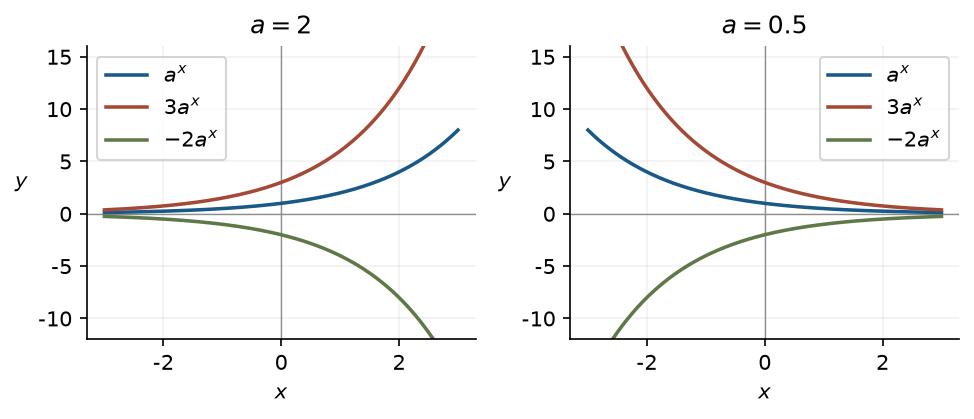
\includegraphics[width=.84\linewidth,height=.38\textheight,keepaspectratio]{figures/C04-HW114-15.png}\end{center}
{\small \field{关联知识}{E01 指数函数的概念、图象与性质（教材帮p.150、151 / PDF159、160）；F09 图象平移、伸缩与对称（教材帮p.86、94 / PDF95、103）}
\field{方法与易错点}{先查底数条件，利用已知点定底数，再据单调性及图象求值或范围。 易错：只要求底数非负；漏排1；将 $a^x+b$ 当标准指数函数且仍用原值域。}
\field{答案依据}{答案册相关题组：PDF第32页（册内页31）；按当前题库原题逐项重算，不按旧版题号机械对套。}}

\clearpage\section{知识点与题目索引}
\par\medskip\noindent\begin{minipage}{\linewidth}\subsection{S01 集合、元素与常用数集}\field{概念要点}{集合元素具有确定性、互异性、无序性。元素与集合用 $\in,\notin$；常用数集 $\mathbb N,\mathbb Z,\mathbb Q,\mathbb R$，其中 $0\in\mathbb N$。有限集可含0个元素，空集 $\varnothing$ 不是 $\{0\}$。含参数元素求解后必须复查互异性。}关联13个条目。代表题：\hyperref[XJ-B1-C01-TH-P002-Y0577]{教材p.2 未编号题组}；\hyperref[XJ-B1-C01-EX-P003-Y0620]{教材p.3 例题1}；\hyperref[XJ-B1-C01-EX-P003-Y1223]{教材p.3 例题2}；\hyperref[XJ-B1-C01-PR-P004-Y0218]{教材p.4 第1题}。\end{minipage}\par
\par\medskip\noindent\begin{minipage}{\linewidth}\subsection{S02 集合表示、区间与数集点集}\field{概念要点}{列举法适合元素有限且可逐项确定的集合；描述法写清代表元素及限制。$[a,b]$ 含两端，$(a,b)$ 不含两端，无穷符号一侧只能用圆括号。$\{x\mid\cdots\}$ 的元素是数，$\{(x,y)\mid\cdots\}$ 的元素是有序数对。}关联12个条目。代表题：\hyperref[XJ-B1-C01-EX-P004-Y1108]{教材p.4 例题3}；\hyperref[XJ-B1-C01-EX-P005-Y0448]{教材p.5 例题4}；\hyperref[XJ-B1-C01-EX-P005-Y1339]{教材p.5 例题5}；\hyperref[XJ-B1-C01-PR-P006-Y0217]{教材p.6 第1题}。\end{minipage}\par
\par\medskip\noindent\begin{minipage}{\linewidth}\subsection{S03 子集、真子集与集合相等}\field{概念要点}{$A\subseteq B$ 表示 $A$ 中每个元素均属于 $B$；真包含还需存在 $B$ 中不属于 $A$ 的元素。$A=B$ 等价于互相包含；空集是任意集合的子集。含 $n$ 个元素的集合有 $2^n$ 个子集、$2^n-1$ 个真子集；非空真子集为 $2^n-2$（$n\ge1$）。}关联11个条目。代表题：\hyperref[XJ-B1-C01-TH-P002-Y0577]{教材p.2 未编号题组}；\hyperref[XJ-B1-C01-TH-P006-Y0849]{教材p.6 未编号题组}；\hyperref[XJ-B1-C01-EX-P007-Y0656]{教材p.7 例题6}；\hyperref[XJ-B1-C01-PR-P008-Y0877]{教材p.8 第1题}。\end{minipage}\par
\par\medskip\noindent\begin{minipage}{\linewidth}\subsection{S04 交集、并集及解集的联系}\field{概念要点}{$x\in A\cap B$ 当且仅当同时属于两集合；$x\in A\cup B$ 当且仅当至少属于一个。交集对应条件“且”，并集对应“或”；乘积为0的解集可取各因式为0的解集之并。数轴上交取公共部分，并取全部覆盖部分。}关联26个条目。代表题：\hyperref[XJ-B1-C01-TH-P009-Y0951]{教材p.9 未编号题组}；\hyperref[XJ-B1-C01-EX-P010-Y0276]{教材p.10 例题9}；\hyperref[XJ-B1-C01-EX-P010-Y0596]{教材p.10 例题10}；\hyperref[XJ-B1-C01-TH-P010-Y1233]{教材p.10 未编号题组}。\end{minipage}\par
\par\medskip\noindent\begin{minipage}{\linewidth}\subsection{S05 全集、补集与德摩根律}\field{概念要点}{$\complement_U A=\{x\in U\mid x\notin A\}$，必须先有 $A\subseteq U$。$A\cap\complement_U A=\varnothing$，$A\cup\complement_U A=U$。$\complement_U(A\cup B)=(\complement_U A)\cap(\complement_U B)$；交的补等于补的并。}关联17个条目。代表题：\hyperref[XJ-B1-C01-TH-P007-Y1130]{教材p.7 未编号题组}；\hyperref[XJ-B1-C01-EX-P008-Y0280]{教材p.8 例题7}；\hyperref[XJ-B1-C01-EX-P008-Y0515]{教材p.8 例题8}；\hyperref[XJ-B1-C01-PR-P008-Y1092]{教材p.8 第3题}。\end{minipage}\par
\par\medskip\noindent\begin{minipage}{\linewidth}\subsection{S06 Venn图、容斥与实际计数}\field{概念要点}{有限集合满足 $|A\cup B|=|A|+|B|-|A\cap B|$。三集合容斥先减两两交集再加三重交集。“只参加两项”不同于“两项都参加”；分区人数均须非负。}关联3个条目。代表题：\hyperref[XJ-B1-C01-HW-P013-Y1051]{教材p.13 第14题}；\hyperref[XJ-B1-C01-HW-P013-Y1531]{教材p.13 第17题}；\hyperref[XJ-B1-C01-RV-P030-Y0883]{教材p.30 第15题}。\end{minipage}\par
\par\medskip\noindent\begin{minipage}{\linewidth}\subsection{L01 命题、真假、逆命题与否定}\field{概念要点}{命题是可判断真假的陈述句。未限定变量的开放语句不一定是命题。“若 $p$ 则 $q$”的逆命题为“若 $q$ 则 $p$”；否定则是原断言不成立，二者不同。原命题与逆命题的真假必须分别判断。本点的完整定义还依据湘教版教材14—16页；《教材帮》30页主要用于条件命题联系。}关联10个条目。代表题：\hyperref[XJ-B1-C01-TH-P014-Y1066]{教材p.14 未编号题组}；\hyperref[XJ-B1-C01-EX-P015-Y0177]{教材p.15 例题1}；\hyperref[XJ-B1-C01-EX-P015-Y0738]{教材p.15 例题2}；\hyperref[XJ-B1-C01-PR-P016-Y0217]{教材p.16 第1题}。\end{minipage}\par
\par\medskip\noindent\begin{minipage}{\linewidth}\subsection{L02 充分、必要、充要条件}\field{概念要点}{$p\Rightarrow q$ 表示 $p$ 是 $q$ 的充分条件，$q$ 是 $p$ 的必要条件；双向成立为充要。只正向为充分不必要，只反向为必要不充分；两向均不成立为既不充分又不必要。解集关系中 $P\subseteq Q$ 对应 $p\Rightarrow q$；$\neg q\Rightarrow\neg p$ 与之等价。}关联18个条目。代表题：\hyperref[XJ-B1-C01-EX-P017-Y0928]{教材p.17 例题3}；\hyperref[XJ-B1-C01-EX-P017-Y1338]{教材p.17 例题4}；\hyperref[XJ-B1-C01-EX-P018-Y0491]{教材p.18 例题5}；\hyperref[XJ-B1-C01-PR-P019-Y0218]{教材p.19 第1题}。\end{minipage}\par
\par\medskip\noindent\begin{minipage}{\linewidth}\subsection{L03 全称、存在量词及真假的判定}\field{概念要点}{$\forall x\in M,p(x)$ 对所有对象断言；$\exists x\in M,p(x)$ 对至少一个对象断言。全称真要证明任意对象，假只需一个反例；存在真只需一个实例，假要证明所有对象都不满足。多个量词的顺序不能随意交换。}关联9个条目。代表题：\hyperref[XJ-B1-C01-TH-P019-Y1033]{教材p.19 未编号题组}；\hyperref[XJ-B1-C01-EX-P020-Y0562]{教材p.20 例题6}；\hyperref[XJ-B1-C01-TH-P020-Y0942]{教材p.20 未编号题组}；\hyperref[XJ-B1-C01-EX-P020-Y1143]{教材p.20 例题7}。\end{minipage}\par
\par\medskip\noindent\begin{minipage}{\linewidth}\subsection{L04 含一个量词命题的否定}\field{概念要点}{$\neg(\forall x\in M,p(x))\Leftrightarrow\exists x\in M,\neg p(x)$；$\neg(\exists x\in M,p(x))\Leftrightarrow\forall x\in M,\neg p(x)$。论域不变，量词交换，断言否定；$\ge$ 的否定为 $<$，$=$ 的否定为 $\ne$。}关联10个条目。代表题：\hyperref[XJ-B1-C01-TH-P021-Y1462]{教材p.21 未编号题组}；\hyperref[XJ-B1-C01-EX-P022-Y0891]{教材p.22 例题9}；\hyperref[XJ-B1-C01-EX-P022-Y1296]{教材p.22 例题10}；\hyperref[XJ-B1-C01-PR-P023-Y0176]{教材p.23 未编号题组}。\end{minipage}\par
\par\medskip\noindent\begin{minipage}{\linewidth}\subsection{I01 不等关系与作差比较}\field{概念要点}{对实数 $A,B$，$A>B\Leftrightarrow A-B>0$。常将差因式分解或配方，利用平方非负定号。差可为0时要保留相等情形；实际不等关系须同时写明字母意义和单位。}关联10个条目。代表题：\hyperref[XJ-B1-C02-TH-P032-Y0904]{教材p.32 未编号题组}；\hyperref[XJ-B1-C02-EX-P034-Y0478]{教材p.34 例题1}；\hyperref[XJ-B1-C02-EX-P034-Y0712]{教材p.34 例题2}；\hyperref[XJ-B1-C02-PR-P034-Y1377]{教材p.34 第1题}。\end{minipage}\par
\par\medskip\noindent\begin{minipage}{\linewidth}\subsection{I02 不等式基本性质与符号条件}\field{概念要点}{不等式同加同减方向不变；同乘除正数保向，负数反向。$a>b,c>d$ 可同向相加；一般不能同向相减相除。正数可保序平方、开方；倒数比较需同号且非0。}关联13个条目。代表题：\hyperref[XJ-B1-C02-TH-P035-Y0319]{教材p.35 未编号题组}；\hyperref[XJ-B1-C02-EX-P037-Y0431]{教材p.37 例题3}；\hyperref[XJ-B1-C02-EX-P037-Y0590]{教材p.37 例题4}；\hyperref[XJ-B1-C02-PR-P037-Y0875]{教材p.37 第1题}。\end{minipage}\par
\par\medskip\noindent\begin{minipage}{\linewidth}\subsection{I03 基本不等式、等号与最值建模}\field{概念要点}{$a,b>0$ 时 $a+b\ge2\sqrt{ab}$，等号当且仅当 $a=b$；$u,v\in\mathbb R$ 时 $u^2+v^2\ge2uv$。定积求和最小、定和求积最大；配凑、拆项、换元后必须复查等号是否在定义域内可取。矩形面积、费用等实际题先列约束。}关联30个条目。代表题：\hyperref[XJ-B1-C02-CA-P033-Y0234]{教材p.33 案例1}；\hyperref[XJ-B1-C02-EX-P039-Y0303]{教材p.39 例题5}；\hyperref[XJ-B1-C02-EX-P039-Y0870]{教材p.39 例题6}；\hyperref[XJ-B1-C02-EX-P039-Y1344]{教材p.39 例题7}。\end{minipage}\par
\par\medskip\noindent\begin{minipage}{\linewidth}\subsection{Q01 二次函数、零点、判别式与根系关系}\field{概念要点}{$a\ne0$ 时，$ax^2+bx+c=a(x+b/(2a))^2-\Delta/(4a)$，$\Delta=b^2-4ac$。$\Delta>0,=0,<0$ 分别对应两个不同零点、一个零点、无零点。实根满足 $x_1+x_2=-b/a,x_1x_2=c/a$。两正根需根存在、和正、积正；若要求相异还需 $\Delta>0$。}关联28个条目。代表题：\hyperref[XJ-B1-C01-PR-P016-Y0217]{教材p.16 第1题}；\hyperref[XJ-B1-C02-TH-P045-Y0479]{教材p.45 未编号题组}；\hyperref[XJ-B1-C02-EX-P046-Y1243]{教材p.46 例题1}；\hyperref[XJ-B1-C02-EX-P047-Y0578]{教材p.47 例题2}。\end{minipage}\par
\par\medskip\noindent\begin{minipage}{\linewidth}\subsection{I04 一元二次不等式与参数分类}\field{概念要点}{$a>0$、两根 $r_1<r_2$ 时，二次式在两根外为正、两根内为负；$a<0$ 反向。严格号排除根，非严格号包含根。$\Delta=0$ 时化平方单独判断，解集可能是空集、单点集、全体实数或挖去一点。含参数时先分二次项为0，再分根的大小。}关联35个条目。代表题：\hyperref[XJ-B1-C02-HW-P049-Y1284]{教材p.49 第7题}；\hyperref[XJ-B1-C02-TH-P050-Y1033]{教材p.50 未编号题组}；\hyperref[XJ-B1-C02-EX-P052-Y0592]{教材p.52 例题1}；\hyperref[XJ-B1-C02-EX-P052-Y1407]{教材p.52 例题2}。\end{minipage}\par
\par\medskip\noindent\begin{minipage}{\linewidth}\subsection{I05 简单分式不等式}\field{概念要点}{先移项通分，使一边为0。$A/B>0\Leftrightarrow AB>0$（自动排除 $B=0$）；$A/B\ge0\Leftrightarrow AB\ge0$ 且 $B\ne0$。不能不明分母符号就直接两边乘分母；约分前排除的点仍须保留限制。}关联4个条目。代表题：\hyperref[XJ-B1-C02-EX-P054-Y1398]{教材p.54 例题4}；\hyperref[XJ-B1-C02-PR-P055-Y1064]{教材p.55 第1题}；\hyperref[XJ-B1-C02-HW-P059-Y0410]{教材p.59 第5题}；\hyperref[XJ-B1-C03-PR-P067-Y1075]{教材p.67 第2题}。\end{minipage}\par
\par\medskip\noindent\begin{minipage}{\linewidth}\subsection{I06 恒成立、有解与范围内最值}\field{概念要点}{$a\ne0$ 时，全域 $ax^2+bx+c>0$ 等价于 $a>0,\Delta<0$；全域 $\ge0$ 则 $a>0,\Delta\le0$。负号对应开口向下。未限定二次时须另查 $a=0$。在区间恒成立转为最小值条件，有解转为相应最大或最小值条件，须检查端点是否可取。}关联6个条目。代表题：\hyperref[XJ-B1-C02-CA-P033-Y0951]{教材p.33 案例2}；\hyperref[XJ-B1-C02-EX-P055-Y0177]{教材p.55 例题5}；\hyperref[XJ-B1-C02-PR-P055-Y1260]{教材p.55 第3题}；\hyperref[XJ-B1-C02-HW-P058-Y1395]{教材p.58 第3题}。\end{minipage}\par
\par\medskip\noindent\begin{minipage}{\linewidth}\subsection{F01 函数本质、构成要素与相同函数}\field{概念要点}{$A,B$ 为非空实数集，对每个 $x\in A$ 在 $B$ 中恰有一个确定值对应才是函数。允许多对一，不允许一对多或某输入无值；值域可真包含于 $B$。相同函数由定义域和对应关系判断，自变量字母可不同。}关联9个条目。代表题：\hyperref[XJ-B1-C03-TH-P065-Y0594]{教材p.65 未编号题组}；\hyperref[XJ-B1-C03-TH-P065-Y1561]{教材p.65 未编号题组}；\hyperref[XJ-B1-C03-EX-P066-Y1436]{教材p.66 例题2}；\hyperref[XJ-B1-C03-PR-P067-Y0874]{教材p.67 第1题}。\end{minipage}\par
\par\medskip\noindent\begin{minipage}{\linewidth}\subsection{F02 定义域与原式限制}\field{概念要点}{分母非0，偶次根式被开方数非负，根式在分母时被开方数严格正；各条件同时满足取交集。零次幂底数非0，负次幂排除0。复合求值还需内层结果进入外层定义域；实际函数加实际范围。}关联16个条目。代表题：\hyperref[XJ-B1-C03-EX-P066-Y0934]{教材p.66 例题1}；\hyperref[XJ-B1-C03-EX-P066-Y1436]{教材p.66 例题2}；\hyperref[XJ-B1-C03-PR-P067-Y1075]{教材p.67 第2题}；\hyperref[XJ-B1-C03-PR-P067-Y1287]{教材p.67 第3题}。\end{minipage}\par
\par\medskip\noindent\begin{minipage}{\linewidth}\subsection{F03 函数求值、解析式与函数建模}\field{概念要点}{$f(a)$ 是输入 $a$ 的输出，$f(a)+1$ 与 $f(a+1)$ 不同。复合求值由内到外；列表、图象先读取内层值。求解析式可用待定系数、换元、配凑或消元。实际建模顺序为设变量、写范围、列关系、求解、解释。}关联52个条目。代表题：\hyperref[XJ-B1-C02-CA-P033-Y0951]{教材p.33 案例2}；\hyperref[XJ-B1-C02-EX-P041-Y0698]{教材p.41 例题8}；\hyperref[XJ-B1-C02-EX-P041-Y1378]{教材p.41 例题9}；\hyperref[XJ-B1-C02-PR-P042-Y1011]{教材p.42 第2题}。\end{minipage}\par
\par\medskip\noindent\begin{minipage}{\linewidth}\subsection{F04 函数三种表示法、图象与读数}\field{概念要点}{列表法突出数据对应，解析法便于精算，图象法呈现变化趋势。作图先查定义域、截距、顶点或转折点，再连接；空心点不属于图象。读图解 $f(x)>g(x)$ 是取 $f$ 曲线在上方的横坐标。数据间插值只是估计，不唯一确定精确函数。}关联29个条目。代表题：\hyperref[XJ-B1-C01-RV-P030-Y1286]{教材p.30 第17题}；\hyperref[XJ-B1-C02-EX-P046-Y1243]{教材p.46 例题1}；\hyperref[XJ-B1-C02-HW-P049-Y0793]{教材p.49 第4题}；\hyperref[XJ-B1-C03-EX-P071-Y1368]{教材p.71 例题5}。\end{minipage}\par
\par\medskip\noindent\begin{minipage}{\linewidth}\subsection{F05 单调性定义、证明与参数}\field{概念要点}{区间 $I$ 内任意 $x_1<x_2$，若 $f(x_1)<f(x_2)$ 则递增，若相反则递减。证明用取值、作差、变形、定号、结论；两个分离区间同向单调不代表并集上单调。二次函数根据开口与对称轴确定单调区间。}关联27个条目。代表题：\hyperref[XJ-B1-C03-PR-P072-Y1416]{教材p.72 第3题}；\hyperref[XJ-B1-C03-TH-P079-Y0868]{教材p.79 未编号题组}；\hyperref[XJ-B1-C03-TH-P081-Y0178]{教材p.81 未编号题组}；\hyperref[XJ-B1-C03-EX-P081-Y0375]{教材p.81 例题1}。\end{minipage}\par
\par\medskip\noindent\begin{minipage}{\linewidth}\subsection{F06 最大值、最小值与值域}\field{概念要点}{最大值需 $f(x)\le M$ 对所有输入成立，且至少一个输入实际取到 $M$；最小值类似。闭区间二次函数比较顶点（在区间内时）与两端点；开端点只有界不一定有最值。值域必须记录所有实际能取到的值。}关联16个条目。代表题：\hyperref[XJ-B1-C03-PR-P072-Y1416]{教材p.72 第3题}；\hyperref[XJ-B1-C03-HW-P077-Y0601]{教材p.77 第6题}；\hyperref[XJ-B1-C03-TH-P079-Y0868]{教材p.79 未编号题组}；\hyperref[XJ-B1-C03-EX-P081-Y1313]{教材p.81 例题2}。\end{minipage}\par
\par\medskip\noindent\begin{minipage}{\linewidth}\subsection{F07 分段函数、绝对值及分段应用}\field{概念要点}{分段函数整体是一个函数。先由输入选择分段再代值；反求输入时须分别求解并与该段范围取交。绝对值按内部为0的点分段。阶梯收费只对超出部分加价；图象各段的端点不能重复给出不同输出。}关联14个条目。代表题：\hyperref[XJ-B1-C03-EX-P074-Y0394]{教材p.74 例题6}；\hyperref[XJ-B1-C03-EX-P075-Y0177]{教材p.75 例题7}；\hyperref[XJ-B1-C03-EX-P075-Y0639]{教材p.75 例题8}；\hyperref[XJ-B1-C03-PR-P076-Y0217]{教材p.76 第1题}。\end{minipage}\par
\par\medskip\noindent\begin{minipage}{\linewidth}\subsection{F08 奇偶性、对称与函数性质应用}\field{概念要点}{定义域先关于原点对称。$f(-x)=f(x)$ 为偶函数，关于 $y$ 轴对称；$f(-x)=-f(x)$ 为奇函数，关于原点对称。奇函数若0有定义则 $f(0)=0$；零函数可既奇又偶。偶函数对称两侧单调方向相反，奇函数对称两侧相同；这不自动给出全域单调性。}关联29个条目。代表题：\hyperref[XJ-B1-C03-TH-P083-Y0277]{教材p.83 未编号题组}；\hyperref[XJ-B1-C03-TH-P083-Y0867]{教材p.83 未编号题组}；\hyperref[XJ-B1-C03-EX-P084-Y0177]{教材p.84 例题4}；\hyperref[XJ-B1-C03-EX-P084-Y0592]{教材p.84 例题5}。\end{minipage}\par
\par\medskip\noindent\begin{minipage}{\linewidth}\subsection{F09 图象平移、伸缩与对称}\field{概念要点}{向右平移 $h$ 得 $y=f(x-h)$，向上平移 $k$ 得 $y=f(x)+k$；$f(-x)$ 关于 $y$ 轴对称，$-f(x)$ 关于 $x$ 轴对称。$cf(x)$ 将纵坐标乘 $c$，$c<0$ 时同时翻折；水平平移同步改变定义域。}关联6个条目。代表题：\hyperref[XJ-B1-C03-RV-P092-Y1067]{教材p.92 第19题}；\hyperref[XJ-B1-C04-TH-P110-Y1359]{教材p.110 未编号题组}；\hyperref[XJ-B1-C04-PR-P113-Y0217]{教材p.113 第1题}；\hyperref[XJ-B1-C04-HW-P113-Y1566]{教材p.113 第6题}。\end{minipage}\par
\par\medskip\noindent\begin{minipage}{\linewidth}\subsection{P01 方根、根式与绝对值}\field{概念要点}{奇数 $n>1$ 时实数 $a$ 有唯一实 $n$ 次方根；偶数 $n$ 时正数有正负两根，根号表示其中非负的算术根。$(\sqrt[n]a)^n=a$（须有意义）；$\sqrt[n]{a^n}=a$（$n$ 奇），$=|a|$（$n$ 偶）。}关联2个条目。代表题：\hyperref[XJ-B1-C04-EX-P095-Y0782]{教材p.95 例题1}；\hyperref[XJ-B1-C04-HW-P104-Y0450]{教材p.104 第1题}。\end{minipage}\par
\par\medskip\noindent\begin{minipage}{\linewidth}\subsection{P02 有理数、实数指数幂与运算}\field{概念要点}{$a>0$ 时 $a^{m/n}=\sqrt[n]{a^m}$，$a^{-r}=1/a^r$；$a^ra^s=a^{r+s}$，$(a^r)^s=a^{rs}$，$(ab)^r=a^rb^r$（按正底数条件使用）。不能把加法的幂拆成幂的和。无理指数幂按有理指数逼近扩充；根式运算中原分母非0等限制不能约掉。}关联25个条目。代表题：\hyperref[XJ-B1-C04-EX-P096-Y0533]{教材p.96 例题2}；\hyperref[XJ-B1-C04-EX-P096-Y0978]{教材p.96 例题3}；\hyperref[XJ-B1-C04-EX-P096-Y1306]{教材p.96 例题4}；\hyperref[XJ-B1-C04-EX-P097-Y0403]{教材p.97 例题5}。\end{minipage}\par
\par\medskip\noindent\begin{minipage}{\linewidth}\subsection{P03 幂函数的概念、图象与性质}\field{概念要点}{幂函数形如 $y=x^\alpha$，底数是自变量，指数为常数，系数为1。正半轴上 $\alpha>0$ 递增、$\alpha<0$ 递减，均过 $(1,1)$；正指数还可在0取0。全域的定义域与奇偶性须依具体指数判断。重点掌握 $x,x^2,x^3,\sqrt x,1/x$，以及由它们推得的负整数、分数指数实例。}关联13个条目。代表题：\hyperref[XJ-B1-C04-EX-P102-Y0177]{教材p.102 例题8}；\hyperref[XJ-B1-C04-EX-P102-Y0669]{教材p.102 例题9}；\hyperref[XJ-B1-C04-PR-P103-Y0797]{教材p.103 第1题}；\hyperref[XJ-B1-C04-PR-P103-Y1012]{教材p.103 第2题}。\end{minipage}\par
\par\medskip\noindent\begin{minipage}{\linewidth}\subsection{E01 指数函数的概念、图象与性质}\field{概念要点}{$y=a^x$ 中 $a>0,a\ne1$，指数是自变量。定义域 $\mathbb R$，值域 $(0,+\infty)$，过 $(0,1)$；$a>1$ 递增，$0<a<1$ 递减。互为倒数的底数对应图象关于 $y$ 轴对称；取 $x=1$ 时纵坐标就是底数。}关联20个条目。代表题：\hyperref[XJ-B1-C04-EX-P099-Y1526]{教材p.99 例题7}；\hyperref[XJ-B1-C04-PR-P100-Y0660]{教材p.100 第3题}；\hyperref[XJ-B1-C04-TH-P109-Y0302]{教材p.109 未编号题组}；\hyperref[XJ-B1-C04-EX-P110-Y0319]{教材p.110 例题3}。\end{minipage}\par
\par\medskip\noindent\begin{minipage}{\linewidth}\subsection{E02 指数式比较、方程与不等式}\field{概念要点}{同底比较用指数函数单调性，底数在 $(0,1)$ 时反向；同指数比较可用正半轴幂函数性质；两者都不同时可搭桥或与1比较。含 $a^{|u(x)|}$ 时先分绝对值或由指数非负判断值域。}关联3个条目。代表题：\hyperref[XJ-B1-C04-EX-P111-Y1422]{教材p.111 例题4}；\hyperref[XJ-B1-C04-PR-P113-Y0347]{教材p.113 第3题}；\hyperref[XJ-B1-C04-HW-P114-Y0711]{教材p.114 第9题}。\end{minipage}\par
\par\medskip\noindent\begin{minipage}{\linewidth}\subsection{E03 指数增长、衰减与实际模型}\field{概念要点}{按固定倍率变化的模型 $M(t)=M_0q^t$。增长率 $r$ 对应 $q=1+r$，衰减率 $r$ 对应 $q=1-r$；半衰期 $T$ 可写 $M(t)=M_0(1/2)^{t/T}$。初始时刻通常为0；细胞分裂、年末计数等还可能限制 $t\in\mathbb N$。}关联9个条目。代表题：\hyperref[XJ-B1-C04-TH-P106-Y0720]{教材p.106 未编号题组}；\hyperref[XJ-B1-C04-EX-P108-Y0177]{教材p.108 例题1}；\hyperref[XJ-B1-C04-EX-P108-Y0840]{教材p.108 例题2}；\hyperref[XJ-B1-C04-PR-P108-Y1273]{教材p.108 第1题}。\end{minipage}\par
\end{document}
